\documentclass[10pt,oneside]{uhthesis}
% \usepackage[showframe]{geometry}
\usepackage{subfigure}
\usepackage[ruled,lined,linesnumbered,titlenumbered,algochapter,spanish,onelanguage]{algorithm2e}
\usepackage{amsmath}
\usepackage{amssymb}
\usepackage{amsbsy}
\usepackage{caption,booktabs}
\captionsetup{
	justification = centering
}
\usepackage[subfigure]{tocloft}
%\usepackage{mathpazo}
\usepackage{float}
% \usepackage{todonotes}
\usepackage{adjustbox}
\usepackage{qtree}
\usepackage{tikz}
\usetikzlibrary{tikzmark,calc,positioning,babel}

\floatstyle{plaintop}
\restylefloat{table}

\renewcommand{\tablename}{Tabla}
\renewcommand{\listalgorithmcfname}{Índice de Algoritmos}%
%\dontprintsemicolon
\SetAlgoNoEnd

% list of definitions
\newcommand{\listdefinitions}{Índice de definiciones}
\newlistof{importantdefinition}{mcf}{\listdefinitions}

% Reset section numbering between unnumbered chapters
% https://tex.stackexchange.com/questions/71162/reset-section-numbering-between
\newcommand{\importantdefinition}[1]
{%
	\refstepcounter{importantdefinition}
	\addcontentsline{mcf}{importantdefinition}
	{\protect #1}\par
%	{\protect\numberline{\theimportantdefinition}#1}\par
}

% end of list of definitions


% list of Codes
\newcommand{\listcodes}{Índice de Códigos}
\newlistof{importantcodes}{mcfc}{\listcodes}

% Reset section numbering between unnumbered chapters
% https://tex.stackexchange.com/questions/71162/reset-section-numbering-between
\newcommand{\importantcodes}[1]
{%
	\refstepcounter{importantcodes}
	\addcontentsline{mcfc}{importantcodes}
	{\protect #1}\par
	%	{\protect\numberline{\theimportantdefinition}#1}\par
}

% end of list of definitions


\title{Métodos de Linealización Local de Orden Superior para problemas de valor inicial de dimensiones no pequeñas}
\author{Lic. Frank Sadan Naranjo Noda}
\advisor{Dr. Juan Carlos Jiménez Sobrino}
\advisorsingle
\degree{Doctor}
\faculty{Facultad de Matemática y Computación}
% \date{}
\logo{Graphics/uhlogo}
\makenomenclature

\newcommand{\nonl}{\renewcommand{\nl}{\let\nl\oldnl}}
\renewcommand{\vec}[1]{\boldsymbol{#1}}
\newcommand{\diff}[1]{\ensuremath{\mathrm{d}#1}}
\newcommand{\me}[1]{\mathrm{e}^{#1}}
\newcommand{\pf}{\mathfrak{p}}
\newcommand{\qf}{\mathfrak{q}}
%\newcommand{\kf}{\mathfrak{k}}
\newcommand{\kt}{\mathtt{k}}
\newcommand{\mf}{\mathfrak{m}}
\newcommand{\hf}{\mathfrak{h}}
\newcommand{\fac}{\mathrm{fac}}
\newcommand{\maxx}[1]{\max\left\{ #1 \right\} }
\newcommand{\minn}[1]{\min\left\{ #1 \right\} }
\newcommand{\lldpcf}{1.25}
\newcommand{\nnorm}[1]{\left\lvert #1 \right\rvert }
\newcommand{\nnnorm}[1]{\left\lVert #1 \right\rVert }
\newcommand{\norme}[1]{\nnorm{\nnorm{ #1 }}_2}
\newcommand{\scal}[2]{\left< #1, #2 \right>}
\newtheorem{example}{Ejemplo}
\newcommand{\redmark}[1]{\textcolor{black}{#1}}
\newcommand{\bluemark}[1]{\textcolor{black}{#1}}
\newcommand{\mmark}[1]{\textcolor{black}{#1}}
\newcommand{\lmatrix}{\mathtt{L}}
\newcommand{\rvector}{\mathtt{r}}

% marker tikz in qtree
\makeatletter
\newcommand{\myLines}[1]{% Three-way only
	\begin{picture}(1,1)
	%	\put(0,0){\line(2,1){2}}
	%	\put(1,0){\vector(0,1){0.7}}
	%	\put(4,0){\line(-2,1){2}}
\end{picture}}
\let\qdrawReal=\qdraw@branches
\newcommand\brOverride{\let\qdraw@branches=\myLines}

\makeatletter
\newcommand{\myLiness}[1]{% Three-way only
	\begin{picture}(4,1)
		\put(0,0){\line(2,1){2}}
		%\put(1,0){\vector(0,1){0.7}}
		\put(4,0){\line(-2,1){2}}
\end{picture}}
\let\qdrawReal=\qdraw@branches
\newcommand\brOverridedd{\let\qdraw@branches=\myLiness}

\newcommand\brRestore{\let\qdraw@branches=\qdrawReal}
\makeatother


\begin{document}

\frontmatter
\maketitle

%\begin{dedication}
\todo[inline]{por escribir la dedicaci\'o}
\end{dedication}
% \begin{acknowledgements}


\end{acknowledgements}
% \begin{opinion}


\end{opinion}
\begin{abstract}
	Las Ecuaciones en Derivadas Parciales (EDP) se utilizan para describir fenómenos físicos, biofísicos y físico-químicos, pero solo se conocen soluciones analíticas para unas pocas EDP lineales. Por lo tanto, se utilizan métodos numéricos, como elementos finitos y diferencias finitas, para aproximar las soluciones. Sin embargo, la mayoría de los integradores numéricos convencionales tienen que solucionar grandes sistemas de ecuaciones algebraicas mal condicionadas, lo que lleva al uso de matrices pre-condicionadoras específicas para cada tipo de EDP. Los integradores exponenciales para las ecuaciones diferenciales ordinarias (EDO), que se obtienen de utilizar el método de las lineas, son una excepción, ya que calculan exponenciales matriciales y/o funciones phi por vectores en lugar de resolver ecuaciones algebraicas. Los integradores exponenciales están disponibles en dos tipos: Globalmente Linealizados (GL) y Localmente Linealizados (LL). Los integradores GL funcionan bien para EDO con términos no lineales pequeños o acotados por la parte lineal, mientras que los integradores LL mejoran a los integradores GL y, en general, a los integradores tradiciones utilizados con el método de las líneas para resolver EDP. Sin embargo, estos integradores involucran el cálculo de varios productos de funciones phi por vector con un alto costo  computacional. La ausencia de una estrategia adaptativa para el tamaño de paso de integración y la necesidad de evaluar la matriz Jacobiana exacta del campo vectorial de la EDO son otras de las limitaciones prácticas de esos métodos. Para EDO de dimensiones pequeñas, los métodos LL de orden superior (LLOS) mejoran la eficacia del método LL clásico de orden 2 al adicionar una aproximación a la representación integral o a la diferencial de su residuo. Los métodos LLOS derivados de la forma diferencial contienen solo un producto de función phi por vector en cada paso de integración, lo que los distingue positivamente de los derivados de la representación integral y motivan la investigación de ésta tesis. 
	
	En la tesis, para EDO de dimensiones no pequeñas, se propone la implementación adaptativa de las fórmulas Runge-Kutta embebidas de Dormand y Prince Localmente Linealizadas, utilizando una aproximación de Krylov de orden superior, una nueva medida de error y una nueva forma de estimar la dimensión óptima de Krylov. También se propone una nueva familia de métodos LLOS Libres de Jacobiano para casos en los que no es viable evaluar y almacenar la matriz Jacobiana de la ODE. Estos métodos utilizan una aproximación de Krylov libre de Jacobiano, una medida de su error y un criterio para estimar la dimensión de Krylov. Se presenta la clase de esquemas de Runge-Kutta Localmente Linealizados Libres de Jacobiano y se construyen explícitamente esquemas de tercer a quinto orden. Además, se implementa un esquema adaptativo de orden variable y libre de Jacobiano utilizando las fórmulas Runge-Kutta embebidas de Dormand y Prince Localmente Linealizadas. Experimentos numéricos muestran la eficacia de nuevos esquemas en la integración de ecuaciones de prueba conocidas y se compara con la de otros integradores exponenciales.
\end{abstract}

\newpage

\begin{center}
	{\large \textbf{Hipótesis}}
\end{center}
¿Es factible aplicar los métodos de Linealización Local de Orden Superior para resolver problemas de valor inicial de dimensiones no pequeñas?

\qquad

\begin{center}
	{\large \textbf{Objetivos de la tesis}}
\end{center}
\textbf{Objetivo general}

Desarrollo de métodos de Linealización Local de Orden Superior para resolver problemas de valor inicial de dimensiones no pequeñas.

\qquad\\
\textbf{Objetivos específicos}

\begin{enumerate}
	\item Desarrollo de aproximaciones Krylov-Padé para la solución de ecuaciones lineales de dimensiones no pequeñas.
	\item Construcción de nuevas fórmulas embebidas de Dormand y Prince localmente linealizadas para problemas de valor inicial de dimensiones no pequeñas.
	\item Desarrollo de métodos de Linealización Local de Orden Superior Libres de Jacobiano
\end{enumerate}

\tableofcontents
\newpage
\listofimportantdefinition
\newpage
\listoffigures
\newpage
\listoftables
\newpage
\listofalgorithms
\newpage
\listofimportantcodes



\mainmatter

%===================================================================================
% Chapter: Introduction
%===================================================================================
\chapter*{Introducción}\label{chapter:introduction}
\addcontentsline{toc}{chapter}{Introducción}
%===================================================================================

Las Ecuaciones en Derivadas Parciales (EDP) son frecuentemente utilizadas para describir la evolución temporal de complejos fenómenos físicos, biofísicos y físico-químicos (ver, por ejemplo, \cite{tikhonov2013,gray1990,cronin1987}), por lo que resulta de gran interés práctico obtener sus soluciones. Sin embargo, las soluciones analíticas explícitas solo son conocidas para unas pocas EDP lineales definidas sobre geometrías simples (ver, por ejemplo, \cite{tikhonov2013}). Por esta razón, típicamente, las soluciones de las EDP son aproximadas mediante algún método numérico. En general, existen varias familias de métodos numéricos entre los que se encuentran los métodos variacionales, los de elementos finitos, los de diferencia finita y los de líneas (ver, por ejemplo, \cite{prenter2008,samarskii2008,schiesser2012}). La gran mayoría de esos integradores numéricos convencionales tienen un inconveniente en común, ellos requieren de la solución de grandes sistemas de ecuaciones algebraicas mal condicionadas y, por lo tanto, necesitan del uso de matrices precondicionadoras específicas para cada tipo de EDP. Como excepción se distinguen los llamados integradores exponenciales para las ecuaciones diferenciales ordinarias (EDO) que resultan de la discretización espacial de las EDP mediante el método de las líneas. En lugar de las mencionadas ecuaciones algebraicas, estos integradores requieren del cálculo de exponenciales matriciales y/o de productos de las llamadas funciones $\varphi$ por vectores que involucran la evaluación de matrices Jacobianas asociadas a la EDO.

Inicialmente, desde principio de los años 60 del siglo pasado, los primeros  integradores exponenciales se derivaron de diferentes aproximaciones a la integral de la fórmula de variación de constantes para la solución de las EDO semilineales resultantes de la discretización espacial de las EDP. Integradores derivados de este enfoque son, por ejemplo, el método de Lawson y Lawson generalizado, la diferenciación temporal exponencial y los métodos exponenciales de Runge-Kutta (ver \cite{Berland07} para una revisión y Capítulo 1 para detalles), y se agrupan dentro de la categoría de integradores exponenciales Globalmente Linealizados~(GL). En general, estos métodos implican el cálculo de exponenciales matriciales y/o de productos de funciones phi por vector solamente en el paso de integración inicial y funcionan bien cuando el término no lineal en las EDO semilineales mencionadas es pequeño o está acotado en términos del término lineal. Sin embargo, cuando el término no lineal es relevante para la dinámica de las EDO semilineales, la efectividad de estos métodos se pierde \cite{hochbruck2009exponential}.


Más recientemente, para solventar la mencionada deficiencia de los integradores GL, se propuso el uso de los llamados integradores de Linealización Local~(LL). Estos métodos se derivan en dos pasos (ver Capítulo 1 para detalles): 1) la linealización local de las mencionadas EDO en cada paso de integración, y 2) una aproximación a la integral de la fórmula de variación de constantes para la solución de la ecuación linealizada del paso 1). A diferencia de los GL, los integradores LL conllevan el cálculo de exponenciales matriciales y/o de productos de funciones phi por vector en cada paso de integración. Integradores de éste tipo son, por ejemplo, el método de propagación iterativa exponencial \cite{tokman2006efficient}, el método exponencial-Rosenbrock \cite{hochbruck2009exponential} y el método exponencial-Adams \cite{hochbruck2011exponential}. Estudios de simulaciones han mostrado que éstos métodos son mucho más eficiente que los integradores tradicionales utilizados con el método de las líneas para resolver EDP. No obstante, el alto orden de convergencia de estos integradores exponenciales conlleva al cálculo de varios productos de funciones $\varphi$ por vector en cada paso de integración lo que conforma la mayor parte  del costo computacional de estos métodos \cite{naranjo2021locally}. La ausencia de una estrategia adaptativa para el tamaño de paso de integración y la necesidad de evaluar la matriz Jacobiana exacta del campo vectorial de la EDO son otras de las limitaciones prácticas de esos métodos.

Por otra parte, con anterioridad a los trabajos mencionados en el párrafo anterior y en un contexto diferente al de la solución de EDP, los integradores de Linealización Local habían sido exitosamente desarrollados para resolver varias clases de sistemas de ecuaciones diferenciales de dimensiones pequeñas \cite{jimenez2020}.
\redmark{Entiéndase por dimensión pequeña aquella de una matriz cuadrada para la cual la aproximación racional de Padé de la exponencial matricial es más eficiente que las aproximaciones iterativas en término del costo computacional.} En el caso específico de EDO, resultados teóricos y de simulaciones muestran que el método LL clásico de orden 2  \cite{pope1963exponential} posee una variedad de propiedades deseables entre las que se encuentran la A-estabilidad, la ausencia de puntos de equilibrio espurios bajo condiciones bastante generales y la preservación del comportamiento dinámico de la solución alrededor de puntos de equilibrio hiperbólicos y órbitas periódicas \cite{Jimenez02AMC}. Si embargo, su bajo orden de convergencia constituye un inconveniente importante. Para solucionar esta limitación \cite{delaCruz06,delaCruz07,Jimenez13}, se propusieron los métodos de Linealización Local de Orden Superior (LLOS) que se obtienen de adicionar al esquema LL clásico de orden 2 una aproximación a la representación integral o a la diferencial de su residuo (ver Capítulo 1 para detalles). Por construcción, los métodos LLOS derivados de la forma diferencial contienen un solo  producto de función phi por vector en cada paso de integración, característica que los distingue muy positivamente de los derivados de la representación integral. Entre los primeros se encuentran los métodos Runge-Kuta Localmente Linealizados de orden 3 y 4, y las fórmulas embebidas Runge-Kutta de Dormand y Prince Localmente Linealizadas \cite{delaCruz06,Jimenez13,Jimenez14AMC}.

Motivado por el hecho de que las fórmulas embebidas Runge-Kutta de Dormand y Prince Localmente Linealizadas comparten un solo producto de función phi por vector en cada paso de integración y, también, por el éxito de su implementación adaptativa para integrar EDO de dimensiones pequeñas, en ésta tesis se valora la posibilidad de construir una implementación adaptativa de dichas fórmulas para integrar sistemas de EDO de dimensiones no pequeñas. Con ese propósito, en las mencionadas fórmulas embebidas, se requiere sustituir la aproximación de Padé para la acción de la función phi sobre un vector por la de algún método iterativo. Basado en el método de los subespacios de Krylov, en trabajos previos se han propuesto varias de esas aproximaciones con diferentes estrategias para controlar sus errores, y varios enfoques para estimar la dimensión de Krylov \cite{hochbruck1998exponential,sidje1998expokit,niesen2012algorithm,gaudreault2018kiops}. Alternativamente, en ésta tesis, se propone una aproximación de orden mayor, una nueva medida del error y una nueva forma de estimar la dimensión óptima de Krylov.

En muchas situaciones prácticas, debido a los insuficientes recursos computacionales disponibles o al uso de discretizaciones espaciales complejas, no es viable evaluar y almacenar la matriz Jacobiana de la EDO u obtener su expresión analítica exacta. Para esos casos, en esta tesis se propone y estudia la nueva familia de métodos LLOS Libres de Jacobiano. Con ese propósito, para el cálculo de los productos de funciones phi por vector se introduce una aproximación de Krylov libre de Jacobiano, una medida de su error y un criterio para estimar la dimensión de Krylov. Como caso particular, se presenta la clase de esquemas de Runge-Kutta Localmente Linealizados Libres de Jacobiano y se construyen explícitamente esquemas de tercer a quinto orden. Modificando las fórmulas embebidas  Runge-Kutta de Dormand y Prince Localmente Linealizadas se implementa un esquema adaptativo de orden variable y libre de Jacobiano.

El documento de tesis está organizado de la siguiente forma. En el primer capítulo se presenta una breve revisión de los integradores exponenciales y los métodos de Linealización Local necesarios para la comprensión de este trabajo. En el segundo capítulo, se construyen las aproximaciones Krylov-Padé con y sin la evaluación del Jacobiano para calcular los productos de funciones phi por vector que representan la solución de EDO lineales, se determinan cotas para dichas aproximaciones y se prueba su efectividad en un conjunto de ecuaciones de prueba. En el Capítulo 3, se derivan las nuevas fórmulas embebidas Runge-Kutta de Dormand y Prince Localmente Linealizadas para EDO de dimensiones no pequeñas y se establece su orden de convergencia. Se presentan también estrategias adaptativas para diseñar tanto esquemas con tamaño de paso fijo y dimensión de Krylov variable, como esquemas con tamaño de paso y dimensión de Krylov variable. En el último capítulo, se introduce una clase de métodos LLOS Libres de Jacobiano y se obtiene un resultado general sobre el orden de convergencia de la nueva familia de integradores. Se introduce, además, la clase particular de esquemas Runge-Kutta Localmente Linealizados Libres de Jacobiano y se modifican las fórmulas embebidas Runge-Kutta  de Dormand y Prince Localmente Linealizadas para implementar un esquema adaptativo de orden variable y libre de Jacobiano.
En los Capítulos 3 y 4, se evalúa el desempeño de los nuevos esquemas en la integración de ecuaciones de prueba conocidas y se compara con otros integradores exponenciales.

Los resultados recopilados en los Capítulos 2, 3 y 4 de la Tesis fueron tomados de artículos \cite{naranjo2021locally,naranjo2023jacobian,naranjo2023computing} publicados por el autor en tres revistas \textit{peer review} con clasificación JCR-Q1 y en los Reportes de Investigación del ICIMAF \cite{naranjo2022RT,naranjo2023RT} con aval de oponentes. Los códigos Matlab que implementan los esquemas de linealizacion local propuestos en la tesis se encuentan disponibles en los repositorios publicos \url{https://github.com/fsadannn/HOLLmethods} y
\url{https://github.com/fsadannn/JF-LLDPschemes}.


\chapter{Integradores exponenciales y método de Linealización Local}\label{chapter:exp-int-and-ll-methods}

En este capítulo se presenta una revisión de la clase general de  integradores numéricos de tipo exponencial y de los Métodos de Linealización Local en particular, así como resultados básicos sobre el cálculo de la exponencial matricial.

En general, se considerarán los problemas de valor inicial definidos por los sistemas de ecuaciones diferenciales no autónomas de la forma
 \begin{equation}
 \frac{dx}{dt}=f(t,x), \;\; \label{ODE-SYST}
 \end{equation}
 \begin{equation*}
 x(t_0)=x_0,
 \end{equation*}
 donde $x_0\in \mathfrak{D}$ es un vector columna inicial dado, $f: [t_0,T] \times \mathfrak{D}\longrightarrow \mathbb{R}^{d}$ es una función vectorial diferenciable, $\mathfrak{D}\subset\mathbb{R}^{d}$ un conjunto abierto, con $d\geq 1$ y $t_0<T \in \mathbb{R}$. Se asumen condiciones de suavidad y condición de Lipschitz en $f$ para asegurar la unicidad de la solución en $\mathfrak{D}$. Denotaremos por $f_x$ la matriz Jacobiana de $f$ respecto a $x$ y por $f_t$ la derivada parcial de $f$ con respecto a $t$.

Consideremos, ademas, una partición $(t)_{h}={t_{n}:n=0,1,\ldots,N}$ del
intervalo $[t_{0},T]$ tal que $t_{0}<t_{1}<\ldots<t_{N}=T$, y $%
h_{n}=t_{n+1}-t_{n}\leq h$; para $n=0,\ldots,N-1$.

\section{Integradores exponenciales} \label{Sec:IE}

En general, se denomina integradores exponenciales a la familia
de esquemas numéricos para EDOs que requieren del cálculo de algún término exponencial. Inicialmente, los integradores de este tipo comenzaron a desarrollarse en los años 60 del siglo pasado~\cite{Berland07} con el propósito de resolver sistemas de ecuaciones semilineales de la forma
\begin{equation}
\frac{dx(t)}{dt} = Ax(t) + F(x(t))  \;\;  \label{ODE Lines Method}
\end{equation}
que resultan de la discretización de una ecuación diferencial en derivadas parciales al utilizar el método de líneas, donde $A$ es una
matriz cuadrada, $F$ una función vectorial no lineal de $x(t)\in\mathbb{R}^d$ y $t\geq t_0 \in \mathbb{R}$. Típicamante, la matriz $A$ en (\ref{ODE Lines Method}) resulta mal condicionada, lo que establece un determinado nivel de rigidez (stiffness en inglés) para ese sistema de ecuaciones \cite{schiesser2012}. La rigidez del sistema (\ref{ODE Lines Method}) se incrementa con la disminución de la distancia entre los puntos de la discretización del método de líneas o con el aumento del número ecuaciones, lo que dificulta su integración con esquemas numéricos explícitos tradicionales \cite{schiesser2012}. Más recientemente, a finales de los años 90, la clase de integradores exponenciales fue extendida a EDOs rígidas (stiff en ingles) de la forma general (\ref{ODE-SYST}).

Los integradores exponenciales tanto para ecuaciones semilineales (\ref{ODE Lines Method}) como para ecuaciones generales (\ref{ODE-SYST}) se derivan de aproximar la integral
que resulta de aplicar la fórmula de variación de constantes a estas ecuaciones~\cite{jimenez2020}. Al aplicar dicha fórmula la solución de la ecuación (\ref{ODE Lines Method}) se escribe como
\begin{equation}
x(t_n+h)=\me{Ah}\left(x(t_n) +\int\limits_{0}^{h} \me{-As}F(x(t_n+s)) \,ds\right)\,. \label{VCF2}
\end{equation}
Los integradores exponenciales obtenidos de aproximar esta expresión son, por ejemplo, los conocidos métodos de Lawson, Lawson Generalizados, Exponential Time
Differencing y Exponential Runge-Kutta (ver \cite{Berland07} para una revisión). Por otra parte, reescribiendo el campo vectorial de (\ref{ODE-SYST}) en la vecindad de ($t_n,x(t_n)$) como la suma de un término lineal y otro no lineal, la fórmula de variación de constantes lleva a
\begin{equation}
x(t_{n}+h) =  x(t_{n})+ \phi(t_{n},x(t_{n});h) + \bluemark{r(t_n,x(t_n);h)} \label{VCF-full}
\end{equation}
con
\begin{equation*}
 \phi(t_{n},x(t_{n});h) = \int\limits_{0}^{h}e^{A_{n}(h-s)}(f(t_n,x(t_{n}))+sf_t(t_n,x(t_{n})))ds 
\end{equation*}
y
\begin{equation}
 \bluemark{r(t_n,x(t_n);h)} =  \int\limits_{0}^{h}e^{A_{n}(h-s)}g_{n}(t_{n}+s,x(t_{n}+s))ds, \label{VCF}
\end{equation}
donde $A_{n}=f_x(t_n,x(t_{n}))$ es la matriz Jacobiana de $f$ evaluada en $(t_n,x(t_{n}))$,  $g_{n}(s,u)=f(s,u)-A_{n}(u-x(t_n))-f_t(t_n,x(t_{n}))(s-t_n)-f(t_n,x(t_n))$ es el término no lineal en la reescritura del campo vectorial de (\ref{ODE-SYST}) y $f_t$ es la derivada parcial de $f$ respecto a $t$. 
Ejemplos de integradores exponenciales obtenidos de aproximar esta expresión son el método clásico de Pope~\cite{pope1963exponential} de orden 2, los métodos Runge-Kutta Localmente 
Linealizados~\cite{delaCruz06,Jimenez13,Jimenez14AMC}, los métodos Exponenciales de Propagación 
Iterativa~\cite{tokman2006efficient, tokman2012new}, los métodos de Taylor Localmente Linealizados~\cite{delaCruz07}, los
métodos Exponenciales tipo Rosenbrok~\cite{hochbruck2009exponential} y los métodos Exponenciales tipo Adams~\cite{hochbruck2011exponential}, todos de orden superior a 2.

En el contexto de las ecuaciones diferenciales de dimensiones pequeñas los integradores exponenciales también fueron tempranamente introducidos como aproximación a las soluciones de dichas ecuaciones. Por ejemplo, para aproximar las ecuaciones diferenciales estocásticas~\cite{ozaki19852,ozaki1985statistical} y sus asociados problemas de filtrado continuo-discreto~\cite{ozaki1993local} y estimación de procesos de difusión~\cite{ozaki19852,ozaki1985statistical,ozaki1994local}. Luego fueron extendidos para la integración de ecuaciones diferenciales aleatorias~\cite{carbonell2005local}, con retardo~\cite{jimenez2006local} y para las parciales estocásticas semilineales~\cite{jentzen2009overcoming,kloeden2011exponential}.

En general, los integradores exponenciales tienen en cuenta que una parte significativa de la estabilidad y las propiedades dinámicas de las ecuaciones diferenciales está contenida en la linealización de la ecuación tratada y se constituyen como una alternativa importante a los métodos implícitos para resolver ecuaciones diferenciales rígidas~(\textit{stiff} en inglés) o altamente oscilatorias.  


\section{Método de Linealización Local}\label{section:ll-methods}
En esta sección se presentan los resultados básicos los Métodos de Linealización Local que se requieren para esta tesis.

\subsection{Aproximación Lineal Local}

El método clásico de Linealización Local de orden 2 de Pope~\cite{pope1963exponential}
 consiste en aproximar en cada paso el campo vectorial de (%
\ref{ODE-SYST}) mediante la expansión de Taylor de primer orden, para
luego resolver exactamente la ecuación lineal resultante. Más
precisamente, si $A_{n}y(t)+a_{n}(t)$ denota la aproximación de Taylor
de primer orden de $f$ en una vecindad de $(t_n,y_{n})$, donde \mbox{$
	A_{n}=f_{x}(t_n,y_{n})$} y $a_{n}(t)=f(t_n,y_{n})-A_{n}y_{n}+f_t(t_n,y_n)(t-t_n)$, entonces la
solución de la ecuación 
\begin{eqnarray}
\frac{dy}{dt} & = & A_{n}y+a_{n}(t) \label{ODE-SYST-LINEAL-1} \\
y(t_{n})& = & y_{n}  \nonumber
\end{eqnarray}
para todo $t\in[t_{n},t_{n+1}]$ es una aproximación de la solución
de (\ref{ODE-SYST}) con condición inicial \mbox{$x(t_{n})=y_{n}$}. Mediante la fórmula de variación de constantes obtenemos 
\begin{equation*}
y(t)=y_{n}+\phi(t_{n},y_{n};t-t_{n})  %\label{ODE-SYST-FORM-LL}
\end{equation*}
donde 
\begin{equation}
\phi(t_{n},y_{n};t-t_{n})=\int\limits^{t-t_{n}}_{0} e^{{A_{n}(t-t_{n}-u)}}
(A_{n}y_{n}+a_{n}(t_{n}+u))\,du.  \label{REV-PHI-DEF-2}
\end{equation}
Aplicando recursivamente la expresión anterior obtenemos la siguiente
definición.

\importantdefinition{Discretización Lineal Local}
\begin{definition}
	\label{definition LLD} Dada una partición $(t)_{h}$, la discretización Lineal Local de la solución de (\ref{ODE-SYST}) está dada por la expresión recursiva
	\begin{equation}
	y_{n+1}=y_{n}+\phi \left( t_{n},y_{n};h_{n}\right) ,  \label{ODE-LLA-4}
	\end{equation}%
	con $y_{0}=x_{0}$, $n=0,1,\ldots,N-1$ y $\phi$ definida en (\ref{REV-PHI-DEF-2}).
\end{definition}

Para todo $t\in[t_{0},T]$ se define la siguiente aproximación.
\importantdefinition{Aproximación Lineal Local}
\begin{definition}
	\label{definition LLA} Dada una partición $(t)_{h}$, la aproximación
	Lineal Local de la solución de (\ref{ODE-SYST}) está dada por 
	\begin{equation}
	y(t)=y_{n_{t}}+\phi(t_{n_{t}},y_{n_{t}};t-t_{n_{t}})
	\label{ODE-REV-FORM-LLA}
	\end{equation}
	para todo $t\in[t_{0},T]$, donde $y_{0}=x_{0}$, $y_{n_{t}}$ es la discretización Lineal Local (\ref{ODE-LLA-4}) y ${n_{t}=\maxx{n:t_{n}\leq t}}$.
\end{definition}
%Otros  integradores que provienen de esta aproximación son~\cite{Jimenez02AMC,Jimenez05AMC}.

 La convergencia, la estabilidad lineal y varias propiedades dinámicas de  la discretización Lineal Local (\ref{ODE-LLA-4}) se pueden encontrar en \cite{Jimenez02AMC}. 
 
 Obsérvese que $\phi$ en la discretización Lineal Local (\ref{ODE-LLA-4}) representa la primera integral de la \bluemark{expresión (\ref{VCF-full})}. De esta forma la integral de la expresión (\ref{VCF}) representa el residuo de dicha aproximación a la solución de la ecuación diferencial (\ref{ODE-SYST}).
\subsection{Aproximación Lineal Local de Orden Superior}

La estabilidad y las propiedades dinámicas que la discretización Lineal Local (\ref{ODE-LLA-4}) posee son de vital importancia para la integración de EDOs, no obstante su bajo orden de convergencia constituye una limitante en algunas circunstancias. Para solucionar esa dificultad se construyen los métodos de Linealización Local de Orden Superior los cuales retienen las propiedades mencionadas, pero con orden de convergencia mayor. 

Estos métodos de Linealización Local de Orden Superior se obtienen de agregar a la aproximación Lineal Local~(\ref{ODE-REV-FORM-LLA}) un término adicional $\widetilde{r}$ que resulta de aproximar, con un orden superior a 2, la integral de la expresión~(\ref{VCF}) por algún método de cuadratura o por la solución numérica de la representación diferencial de la integral~(\ref{VCF})~\cite{delaCruz06}. \bluemark{Utilizando} diferentes tipos de cuadraturas para aproximar~(\ref{VCF}) se obtienen los métodos Exponenciales de Propagación 
Iterativa~\cite{tokman2006efficient}, los métodos de Taylor Localmente Linealizados~\cite{delaCruz07}, los
métodos Exponenciales tipo Rosenbrok~\cite{hochbruck2009exponential} y los métodos Exponenciales tipo Adams~\cite{hochbruck2011exponential}. Por otra parte, \bluemark{utilizando} esquemas Runge Kutta (RK) para resolver la mencionada ecuación diferencial se obtienen los métodos Runge-Kutta Localmente Linealizados~\cite{delaCruz06,Jimenez13,Jimenez14AMC}.

Por su relevancia en esta tesis, a continuación se expondrá con mas detalle los métodos Runge-Kutta Localmente Linealizados. 
\importantdefinition{Aproximación Lineal Local de Orden Superior}
Dada una partición $(t)_{h}$, una aproximación Lineal Local de orden $%
\gamma$ de la solución de (\ref{ODE-SYST}) se define por la expresión~\cite{Jimenez13}
\begin{equation}
y(t)=y_{n_{t}}+\phi(t_{n_{t}},y_{n_{t}};t-t_{n_{t}})+\widetilde{r}(t,t_{n_{t}},y_{n_{t}}),
\label{ODE-REV-HOLL}
\end{equation}
donde ${n_{t}=\maxx{n:t_{n}\leq t}}$, $\widetilde{r}(t,t_{n_{t}},y_{n_{t}})$ es la solución numérica de orden $\gamma >2$ de la \bluemark{representación diferencial de la integral~(\ref{VCF})}
\begin{eqnarray}
\frac{dr}{dt} & = & q(t_{n},y_{n},t,r(t))  \label{ODE r} \\
r(t_{n}) & = & 0 \nonumber
\end{eqnarray}
para todo $t\in [t_{n},t_{n+1})$, con campo vectorial 
\begin{eqnarray*}
q(t_n,y_n,s,\varsigma)&=&f(s,y_n+\phi(t_n,y_n;s-t_n)+\varsigma)-f_x(t_n,y_n)\phi(t_n,y_n;s-t_n)-f(t_n,y_n)%\\
% & &-f_t(t_n,y_n)(s-t_n) -f(t_n,y_n) ,
%\label{AUX-ODE}
\end{eqnarray*}
con $s\in [t_{n},t_{n+1})$ y $\varsigma \in \mathbb{R}^d $. Aquí, la ecuación (\ref{ODE r}) resulta de derivar (\ref{VCF}) con respecto a t. 

Cuando $\widetilde{r}$ en (\ref{ODE-REV-HOLL})  es la aproximación obtenida mediante un esquema Runge-Kutta de orden $\gamma$ se llega a las definiciones siguientes.
\importantdefinition{Discretización Lineal Local Runge-Kutta}
\begin{definition}
	\label{definition HLLD} \cite{Jimenez13} Dada una partición $(t)_{h}$, la discretización Lineal Local Runge-Kutta 
    de orden $\gamma >2$ se define por la expresión recursiva:
	\begin{equation*}
	y_{n+1}=y_{n}+\phi \left( t_{n},y_{n};h_{n}\right) +h_{n}\sum_{j=1}^{s}b_{j}\kt_{j}
	%\label{LLRK_Discretizat}
	\end{equation*}%
	con $y_{0}=x_{0}$, donde las constantes $b_{j}$ y las funciones $k_{j}$ están definidas por el método Runge-Kutta de $s$ estados aplicado a la ecuación~(\ref{ODE r}).
\end{definition}
\importantdefinition{Aproximación Lineal Local Runge-Kutta}
\begin{definition}
	\label{definition HOLLA} \cite{Jimenez13} Dada una partición $(t)_{h}$, la aproximación Lineal Local Runge-Kutta de orden $\gamma$ se define por 
	\begin{equation*}
	y(t)=y_{n_{t}}+\phi(t_{n_{t}},y_{n_{t}};t-t_{n_{t}})+(t-t_{n_{t}})%
	\sum_{j=1}^{s}b_{j}\kt_{j}(t_{n_{t}},y_{n_{t}},t-t_{n_{t}}) %\label{LLRK_Approx}
	\end{equation*}
	para todo $t\in[t_{0},T]$, donde $y_{n_{t}}$ es la discretización Lineal Local Runge-Kutta de orden $\gamma$, y $n_{t}=\maxx{n:t_{n}\leq t}$.
\end{definition}

Como ejemplos importantes se tienen las siguientes discretizaciones Lineales Locales Runge-Kutta de orden 4 y 4-5.

Utilizando la fórmula Runge-Kutta clásica de orden 4~\cite{hairer1993solving} para integrar la ecuación auxiliar (\ref{ODE r}), se obtiene la discretización Lineal Local Runge-Kutta de orden 4~\cite{Jimenez13}:

\begin{equation}
    y_{n+1}\,=\,y_n+\phi(t_n,y_n;h_n)+\frac{h_n}{6}(2\kt_2+2\kt_3+\kt_4)
    \label{LL-scheme-4}
\end{equation}
con
    \[ \kt_j = f\left( t_n+c_jh_n\, , \, y_n+\phi(t_n,y_n;c_jh_n)+c_jh_n\kt_{j-1} \right)
- f_x(t_n\, , \, y_n)\phi(t_n,y_n;c_jh_n) - f(t_n\, ,\, y_n) ,\]
donde $\kt_1=0$ y $c = \left[ 0 \; \frac{1}{2} \; \frac{1}{2} \; 1  \right]$.

Si se utilizan las fórmulas embebidas Runge-Kutta de Dormand y Prince para integrar la ecuación auxiliar (\ref{ODE r}), entonces se obtiene la discretización embebida Lineal Local Runge-Kutta~\cite{Jimenez14AMC}
\begin{equation}
y_{n+1}\,=\,y_n+\phi_s+h_n \sum_{j=1}^{s}b_j \kt_j \quad \text{y} \quad
\widehat{y}_{n+1}\,=\, y_n+\phi_s+h_n \sum_{j=1}^{s}\widehat{b}_j \kt_j
\label{LLDP-scheme-dp}
\end{equation}
de orden 5 y 4, donde $s = 7$ es el número de estados,
\[ \kt_j = f\left( t_n+c_jh_n\, , \, y_n+\phi_j+h_n \sum_{i=1}^{j-1}a_{j,i}\kt_i \right)  
- f_x(t_n\, , \, y_n)\phi_j - f(t_n\, ,\, y_n),\]
\[ \phi _j = \phi \left( t_{n},y_{n};c_jh_{n}\right), \]
y coeficientes Runge-Kutta $a_{j,i}$, $b_j$, $\hat{b}_j$ y $c_j$ definidos en Tabla \ref{ButcherTabla}.


\begin{table}[h]
	\caption{Butcher tableau para los coeficientes de las fórmulas Runge-Kutta embebidas de Dormand y Prince~\cite{hairer1993solving}} \label{ButcherTabla}
	\begin{center}
		\begin{tabular}{ l@{\vrule height 5pt depth 10pt width 0pt}|lllllll}
			$0$ & \\
			$\frac{1}{5}\quad$ & $\frac{1}{5}$ \\
			$\frac{3}{10}\quad$ & $\frac{3}{40}$ & $\frac{9}{40}$ \\
			$\frac{4}{5}\quad$ & $\frac{44}{45}$ & $-\frac{56}{15}$ & $\frac{32}{9}$ \\
			$\frac{8}{9}\quad$ & $\frac{19372}{6561}$ & $-\frac{25360}{2187}$ & $\frac{64448}{6561}$ & $-\frac{212}{729}$ \\
			$1\quad$ & $\frac{9017}{3168}$ & $-\frac{355}{33}$ & $\frac{46732}{5247}$ & $\frac{49}{176}$
			& $-\frac{5103}{18656}$ \\
			$1\quad$ & $\frac{35}{384}$ & $0$ & $\frac{500}{1113}$ & $\frac{125}{192}$
			& $-\frac{2187}{6784}$ & $\frac{11}{84}$ \\
			\hline
			$\widehat{y}$ & $\frac{5179}{57600}$ & $0$ & $\frac{7571}{16695}$ & $\frac{393}{640}$
			& $-\frac{92097}{339200}$ & $\frac{187}{2100}$ & $\frac{1}{40}$
			\rule[-0.3cm]{0cm}{0.8cm} \\
			$y$ & $\frac{35}{384}$ & $0$ & $\frac{500}{1113}$ & $\frac{125}{192}$
			& $-\frac{2187}{6784}$ & $\frac{11}{84}$ & $0$
		\end{tabular}
	\end{center}
\end{table}

En síntesis, a la clase de métodos de Linealización Local de Orden Superior pertenecen los integradores numéricos derivados de dividir, en intervalos de tiempo consecutivos, la solución $x$ de la ecuación original en dos partes: la solución $u$ de la ecuación linealizada localmente más una solución aproximada a la representación diferencial del residuo $r = x-u$ proporcionada por un integrador numérico de orden alto. La Figura \ref{fig:ll-graph} muestra una representación gráfica de esta explicación. 
\begin{figure}
%	\qtreeshowframes
	\begin{center}
		\leaf{\small \tikzmark{c} Aproximación $\widetilde{u}$  \tikzmark{d} }
		\branch{1}{\small EDO lineal asociada a $u$\\$\frac{du(t)}{dt} = a(x(t_n);u(t))$\\$u(t_n)=x(t_n)$\\$a(x_n;\xi) = f_x(x_n)(\xi-x_n)+f(x_n)$}
		\brOverride
		\leaf{ \tikzmark[top]{a} $\widetilde{y}_{n+1} = \widetilde{u}(t_{n},\widetilde{y}_n)+\widetilde{r}(t_{n},\widetilde{y}_n)$  \tikzmark[top]{b}\\
		$\widetilde{y_0}=x(t_0)$}
		\branch{1}{ \\ \\ \\ \\ \\ \\ \\ \\ \\ \\}
		\brRestore
		\leaf{\small \tikzmark{e} Aproximación $\widetilde{r}$ \tikzmark{f}}
		\branch{1}{\small EDO no lineal asociada a $r$\\$\frac{dr(t)}{dt} = q(x(t_n);t,r(t))$\\$r(t_n)=0$\\
			$q(x_n;s,\xi)=f(u(s;x_n)+\xi)$\\
			 $-f_x(x_n)(u(s;x_n)-x_n)$\\
			$-f(x_n)$
		}
		\brOverridedd
		\branch{3}{$ x(t_{n+1}) = u(t_{n},x(t_n))+r(t_{n},x(t_n))$}
		\brRestore
		\branch{1}{\footnotesize $\frac{dx}{dt}=f(x(t_n))+f_x(x(t_n))(x(t)-x(t_n))+\left[ f(x(t))-f(x(t_n))-f_x(x(t_n))(x(t)-x(t_n))  \right]$\\$ t\in[t_{n},t_{n+1}]$}
		\branch{1}{$\frac{dx}{dt}=f(x),\; x(t_0)=x_0\;,\; t\geq t_0$}
		\qobitree
	\end{center}
	\begin{tikzpicture}[overlay, remember picture]
		\draw [-, shorten >=22pt, shorten <=10pt] ($(pic cs:c)!1/2!(pic cs:d)$) -- ($(pic cs:a)!1/2!(pic cs:b)$);
		\draw [-, shorten >=28pt, shorten <=12pt] ($(pic cs:e)!1/2!(pic cs:f)$) -- ($(pic cs:a)!1/2!(pic cs:b)$);
	\end{tikzpicture}
	\caption{Representación gráfica de la descomposicion Lineal Local (\ref{VCF-full}) de la solución x de una ecuacion diferencial ordinaria, y de un esquema de  Linealización Local de Orden Superior $\widetilde{y}_{n+1}$.}
	\label{fig:ll-graph}
\end{figure}


\subsection{Esquemas de Linealización Local}

Como puede notarse de las Definiciones \ref{definition LLD},\ref{definition HLLD} , las
discretizaciones Lineales Locales no pueden ser implementadas directamente por
estar expresadas en término de integrales o ecuaciones diferenciales que en general no pueden ser
calculadas analíticamente. Dependiendo de la forma de calcular  numéricamente esas integrales,
 diferentes esquemas numéricos pueden ser obtenidos \cite{Jimenez05AMC,Jimenez13}.
 Más precisamente tenemos la siguiente definición.
 \importantdefinition{Esquema de Linealización Local}
\begin{definition}
	\label{definition LLS} Dada la discretización Lineal Local 
	  $y_n=y_{n}+\digamma(t_{n},y_{n},t-t_{n})$
	 de orden $\gamma $, toda fórmula recursiva de la forma 
	\begin{equation*}
	 \widetilde{y}_{n+1}=\widetilde{y}_{n}+\widetilde{\digamma}(t_{n},\widetilde{y}_{n},t-t_{n})
	 , \text{ \ \ \ \
		\ con }\widetilde{y}_{0}=y_{0},
	\end{equation*}%
	donde $\widetilde{\digamma}$ denota una aproximación
	de $\digamma$ mediante un algoritmo numérico, es
	llamada genéricamente esquema de Linealización Local (LL).
\end{definition}
\importantdefinition{Esquema de Linealización Local de Orden Superior}
Regularmente, en la literatura, la implementación numérica de la discretización Lineal Local~(\ref{ODE-LLA-4}) se denomina simplemente esquema de Linealización Local, mientras que la implementación numérica de una aproximación de orden superior como la~(\ref{ODE-REV-HOLL}) se denomina esquema de Linealización Local de Orden Superior (LLOS).

Por ejemplo, cuando la fórmula de Padé con escalamiento y potenciación para exponenciales matriciales \cite{moler2003nineteen} es utilizada para
aproximar $\phi$ en la discretización Lineal Local~(\ref{ODE-LLA-4}) se obtiene el esquema LL de orden $2$ \cite{Jimenez02AMC}:
\begin{equation} 
\widetilde{y}_{n+1}=\widetilde{y}_{n}+\widetilde{\phi}\left( t_{n},\widetilde{y}_{n};h_{n}\right) \label{LL-scheme}
\end{equation} 
donde $\widetilde{\phi }\left( t_{n},\widetilde{y}
_{n},h_{n}\right) =\lmatrix\,(P_{\pf,\qf}(2^{-k_{n}}\widetilde{M}_{n}h_{n}))^{2^{k_{n}}}\rvector$, 
$(P_{\pf,\qf}(2^{-k_{n}}\widetilde{M}_{n}h_{n}))^{2^{k_{n}}}$ es la aproximación
de Padé de orden $(\pf,\qf)$ de  $\me{\widetilde{M}_{n}h_{n}}$, donde
$k$ es el menor número natural tal que $\left\Vert 2^{-k_{n}}\widetilde{M}_{n}h_{n}\right\Vert \leq \frac{1}{2}$, 
y las matrices $\widetilde{M}_{n}$, $\lmatrix$, $\rvector$ están definidas como

\begin{equation*}
\widetilde{M}_{n}=\left[ 
\begin{array}{ccc}
f_{x}(t_{n},\widetilde{y}_{n}) &f%
_{t}(t_{n},\widetilde{y}_{n}) & f(t_{n},\widetilde{
		y}_{n}) \\ 
0 & 0 & 1 \\ 
0 & 0 & 0%
\end{array}%
\right] \in \mathbb{R}^{(d+2)\times (d+2)},
\end{equation*}%
$\lmatrix=\left[ 
\begin{array}{ll}
I_{d} & 0_{d\times 2}%
\end{array}%
\right] $ y $\rvector^{\intercal }=\left[ 
\begin{array}{ll}
\mathbf{0}_{1\times (d+1)} & 1%
\end{array}%
\right] $ para EDOs no autónomas; y 
\begin{equation*}
\widetilde{M}_{n}=\left[ 
\begin{array}{cc}
f_{x}(t_{n},\widetilde{y}_{n}) & f(t_{n},%
\widetilde{y}_{n}) \\ 
0 & 0%
\end{array}%
\right] \in \mathbb{R}^{(d+1)\times (d+1)},
\end{equation*}%
$\lmatrix=\left[ 
\begin{array}{ll}
I_{d} & 0_{d\times 1}%
\end{array}%
\right] $ y $\rvector^{\intercal }=\left[ 
\begin{array}{ll}
\mathbf{0}_{1\times d} & 1%
\end{array}%
\right] $ para ecuaciones autónomas.

Por otra parte, cuando la mencionada aproximación de Padé se utiliza para aproximar $\phi$ y $\phi_j$ en las discretizaciones~(\ref{LL-scheme-4}) y~(\ref{LLDP-scheme-dp}) se obtienen los esquemas LLOS propuestos en \cite{Jimenez13,Jimenez14AMC} orientados a resolver problemas de valor inicial de dimensiones pequeñas. La Figura \ref{fig:ll-graph} muestra una representación gráfica resumida de como se construyen esquemas LLOS en general. 

\section{Cálculo de la exponencial de una matriz}

\begin{definition}
    \label{EXPM}\cite{golub2013matrix} Sea $A$ una matriz de $n\times n$ real o compleja. La exponencial de $A$ denotada por
    $ \me{A} $ o $\mathrm{exp}(A)$ es una matriz de $n\times n$ dada por la serie de potencias
    \[\me{A}=\sum_{k=0}^{\infty}\frac{1}{k!}A^{k}.\]
\end{definition}
En muchas aplicaciones se utiliza $\me{tA}$ donde $t$ es un escalar, por tanto 
\begin{equation}
\me{tA}=I+tA+\frac{t^{2}A^{2}}{2!}+\cdots\label{EXPM-SERIE}
\end{equation}
\begin{theorem}\cite{IntroMatrix}
    La serie de matrices definida en~(\ref{EXPM-SERIE}) existe para toda matriz $A$ para $t$ fijo y
    para todo $t$ para $A$ fija. La serie converge uniformemente en cualquier región de t del plano complejo.
\end{theorem}

En \cite{golub2013matrix} se presenta una revisión de los métodos numéricos
para aproximar
la exponencial de matrices. Los métodos más utilizados son la aproximación de Padé con escalamiento
y potenciación para matrices pequeñas y densas, y el de los subespacios de Krylov para matices grandes y esparcidas.


\subsection{Aproximación de Padé}\label{section:pade-approx}
\importantdefinition{Aproximación de Padé}
\begin{definition}
    \cite{golub2013matrix}~La aproximación racional de Padé $P_{\pf,\qf}(z)$
    de $\me{z}$ está dada por 
    \begin{equation*}
    P_{\pf,\qf}(z)=D_{\pf,\qf}(z)^{-1}N_{\pf,\qf}(z),  \label{FORM PADE}
    \end{equation*}%
    donde 
    \[
    N_{\pf,\qf}(z)=\sum\limits_{k=0}^{\pf}\frac{(\pf+\qf-k)!\pf!}{(\pf+\qf)!k!(\pf-k)!}z^k
    \]%
    y 
    \[
    D_{\pf,\qf}(z)=\sum\limits_{k=0}^\qf\frac{(\pf+\qf-k)!\qf!}{(\pf+\qf)!k!(\qf-k)!}(-z)^k
    \]
\end{definition}

Cuando la norma de \mmark{una} \redmark{matriz cuadrada} $A$ es grande, el costo computacional y los errores de redondeo \mmark{en $P_{\pf,\qf}(A)$} aumentan, por lo que
es necesaria la alternativa de escalamiento y potenciación.

\begin{definition}\cite{golub2013matrix}~
    Sea $A$ una matriz cuadrada, y sea $P_{\pf,\qf}(2^{-k}A%
    )$ la aproximación de Padé de orden $(\pf,\qf)\ $de $\me{2^{-k}A%
    }$, donde $k$ es el menor número natural tal que $\left\vert 2^{-k}A%
    \right\vert \leq \frac{1}{2}$. \ Se define la aproximación de  Padé-$(\pf,\qf)$ con escalamiento y potenciación como 
    \begin{equation}
    F_{k}^{\pf,\qf}(A)=(P_{\pf,\qf}(2^{-k}A))^{2^{k}}.
    \label{P-MA-2}
    \end{equation}
\end{definition}

Resultados sobre el error y la estabilidad de las aproximaciones de Padé se presentan a continuación.

\begin{theorem}
    \label{Conv. Pade}\cite{jimenez2012convergence} El error
    relativo y absoluto de la aproximación de Padé con escalamiento y
    potenciación (\ref{P-MA-2}) de $\me{A}$ está dado por: 
    \[
    \frac{\left\vert e^{A}-F_{k}^{\pf,\qf}(A)\right\vert 
    }{\left\vert e^{A}\right\vert }\leq \epsilon _{p,q}\left\vert 
    A\right\vert e^{\epsilon _{p,q}\left\vert A\right\vert }
    \]%
    y 
    \begin{equation}
    \left\vert \me{A}-F_{k}^{\pf,\qf}(A)\right\vert \leq
    c_{p,q}(k,\left\vert A\right\vert )\left\vert A\right\vert
    ^{p+q+1}, \label{errpade}
    \end{equation}
    donde $\epsilon _{p,q}=\alpha (\frac{1}{2})^{p+q-3}$, $%
    c_{p,q}(k,\left\vert A\right\vert )=\alpha
    2^{-k(p+q)+3}\me{(1+\epsilon _{p,q})\left\vert A\right\vert }$ y $%
    \alpha =\frac{p!q!}{(p+q)!(p+q+1)!}$.
\end{theorem}

\begin{theorem}\label{Stab. Pade}[Teorema 4.12 en \cite{wanner1996solving}] 
    La aproximación de Padé $P_{\pf,\qf}(z)$  es \emph{A-estable} si y solo si $\pf\leq \qf\leq \pf+2$. 
    Todos los ceros y todos los polos son simples.
\end{theorem}

\subsection{Aproximación de Krylov}

Los estudios muestran que la aproximación de Padé con escalamiento y potenciación
es efectiva para calcular exponenciales de matrices relativamente pequeñas y densas; pero no así para matrices de dimensiones moderadas o grandes \cite{moler2003nineteen}.

Es conocido del Álgebra Lineal Numérica que para problemas de
grandes dimensiones los métodos iterativos son preferidos por sobre los métodos directos.
En particular,
los métodos iterativos de los subespacios de Krylov han cobrado auge en la resolución de
problemas del Álgebra Lineal que involucran el producto de una función matricial y un vector,
tales como la resolución de grandes sistemas lineales y en el cálculo de valores
propios~\cite{golub2013matrix}.

Es importante destacar que en la mayoría de los integradores exponenciales
 no se necesita el cálculo de la matriz $\me{A}$ completa, sino
el producto $\me{A}b$ donde $b$ es un vector determinado. Por ejemplo, la solución del problema de valor inicial homogéneo $\dot{x}(t)=Ax(t),\;x(0)=x_0$, es $x(t)=\me{At}x_0$ en forma de producto exponencial de matriz y vector. 
\importantdefinition{$\mf$-ésimo subespacio de Krylov}
\begin{definition}
        \cite{Saad92} Para $\mf\geq 1$, el $\mf$-ésimo subespacio de Krylov de la matriz $A\in\mathbb{C}^{N\times N}$
    y el vector $b\in\mathbb{C}^{N}$ se define como
    \[ \mathcal{K}_\mf(A,b)=\mathrm{span}\left\{ b,Ab,A^{2}b,\ldots,A^{\mf-1}b \right\}. \]
\end{definition}

Antes de definir la aproximación por subespacios de Krylov del producto de una función matricial y un vector es
necesario construir una base ortonormal. Para construir dicha base se utiliza el algoritmo de
Arnoldi~\ref{alg:Arnoldi} para matrices generales y el algoritmo de 
Lanczos para matrices hermíticas~\cite{arnoldi,saad2003iterative}.

\begin{algorithm}
    \caption{Algoritmo de Arnoldi para construir una base ortonormal $\{ v_1,\ldots,v_\mf \}$ del $\mf$-ésimo subespacio de Krylov $\mathcal{K}_\mf(A,b)=\mathrm{span} \{ b,Ab,\ldots, A^{\mf-1}b \}$}
    \label{alg:Arnoldi}
    \KwIn{Matriz $A\in \mathbb{R}^{d\times d}$ y vector $b\in \mathbb{R}^{d}$}
    \KwOut{$V_\mf=\left[ v_1 \, \cdots \, v_\mf \right]\in\mathbb{R}^{d\times\mf}$, matriz de Hessenberg $H_\mf^*=V_\mf^{\intercal}A V_\mf $, $v_{\mf}\in\mathbb{R}^d$, $\hf_{\mf+1,\mf}$, $\mf_{cut}$, $breakdown$ }

    $breakdown=false$\\
    $v_1=b/\lVert b \rVert_2$\\
    \For{ $j=1,2,\ldots,\mf$ }{
        $w_j= A v_j$\\
        \For{ $i=1,\ldots,j$}{
            $\hf_{ij}=\langle w_j,v_i \rangle$\\
            $w_j=w_j-\hf_{ij}v_i$
        }
        $\hf_{j+1,i}=\lVert w_j \rVert_2$\\
        \eIf(\tcp*[h] \emph{Break Down}\label{alg:breakdown}){$\hf_{j+1,i}<2\epsilon_{mach}$}{
            $\mf_{cut}=j$\\
             $breakdown=true$\\
            Stop
        }{
            $v_{j+1}=w_j/\hf_{j+1,i}$
        }
    }
\nonl $\epsilon_{mach}$ denota el espaciamiento del numero en punto flotante 1 y $\langle . , .\rangle$ denota producto escalar
\end{algorithm}


\begin{definition}
    \cite{Saad92} Sea $V_\mf$ una base ortonormal de $\mathcal{K}_\mf(A,b)$ y sea $f$ una función matricial definida
    en el espectro de $A$. La aproximación de $f(A)b$ por el  $\mf$-ésimo subespacio de Krylov se define
    \begin{equation}
        f(A)b\approx ||b||_2 V_\mf f(H^*_\mf)e_1, \label{MFUNC-APROX}
    \end{equation}
    donde $H_\mf^*=V_\mf^{\intercal}AV_\mf$ y $e_1$ es el primer vector canónico de $\mathbb{R}^\mf$.
\end{definition}
Cuando la función $f$ en~(\ref{MFUNC-APROX}) es la exponencial matricial se obtiene el siguiente resultado.
\begin{theorem}\label{exp-bound}
	\cite{Saad92} Sea $A\in\mathbb{C}^{N\times N}$ una matriz. El error de aproximación de $\me{A}b$ por el $\mf$-ésimo subespacio
	de Krylov es
	\begin{equation*}
	\left\lvert\left\lvert \me{A}b - \lvert\lvert b \rvert\rvert_2 V_\mf\me{H^*_\mf}e_1 \right\rvert\right\rvert_2 
	\leq \frac{2\vert\lvert b \rvert\rvert_2 \left( \sigma(A) \right)^{\mf}\me{\sigma(A)}}{\mf!},
	\end{equation*}
	donde $\sigma(A)$ es el radio espectral de $A$.
\end{theorem}

\section{Producto de funciones phi por vectores}\label{section:phi-times-vector}

Como se explicó en la Sección \ref{Sec:IE}, los integradores exponenciales resultan de aproximar las expresiones (\ref{VCF2}) o (\ref{VCF-full}). Al utilizar polinomios en $s$ para aproximar las funciones $F$, $\phi$ y $g$ en (\ref{VCF2}) o (\ref{VCF-full}), típicamente, se obtienen expresiones recursivas que involucran integrales de la forma
\begin{equation*}
\phi _{k}(z,h)=\int_{0}^{h}e^{z(h-s)}s^{k-1}ds,\text{ \ \ \ \ \ \ \ }%
k=1,2,\ldots ,
\end{equation*}%
o, equivalentemente, su versión escalada
\begin{equation*}
\varphi _{k}(z)=\int_{0}^{1}e^{z(1-\theta )}\frac{\theta ^{k-1}}{(k-1)!}%
d\theta ,\text{ \ \ \ \ \ \ \ }k=1,2,\ldots ,
\end{equation*}%
- llamada función phi - que resulta de la relación trivial 
\begin{equation}
	\phi _{k}(z,h)=(k-1)!h^{k}\varphi_{k}(hz) \label{phi-vphi-relation}
\end{equation} 
donde $\phi _{0}(z,h)=\varphi _{0}(hz)=e^{hz}$. Por ejemplo, utilizando la relación (\ref{phi-vphi-relation}), la discretización Lineal Local (\ref{ODE-LLA-4})
puede reescribirse como
\begin{equation}
		y_{n+1}=y_{n}+h_n\varphi_1(h_nf_x(t_n,y_n))f(t_n,y_n) + h_n^2\varphi_2(h_nf_x(t_n,y_n))f_t(t_n,y_n)  \, . 
\end{equation}


Otras definiciones comunes de las funciones phi como operador son \cite{Saad92}
\begin{eqnarray}\label{phi-definition}
\varphi_{k+1}(z) &=& \frac{\varphi_k(z)-\varphi_k(0)}{z}, \label{DEF-PHI}\\
\varphi_k(z) & = &\sum\limits_{j=0}^{\infty}\frac{z^{j}}{(k+j)!}, \nonumber 
\end{eqnarray}
para todo $k=1,2,\ldots$.

En general, para el producto de funciones $\varphi_k$ por vector se establece la expansión en serie \cite{Saad92,sidje1998expokit}
\begin{equation} \label{PHI-EXPANSION}
	\varphi_k(\tau A)b=||b||_2\tau^{k} V_\mf \varphi_k(\tau H_\mf)e_1 + ||b||_2\hf_{\mf+1,\mf}
	\sum_{j=k+1}^{\infty}\tau^{j} e_\mf^T\varphi_j(\tau H_\mf)e_1A^{j-k-1}v_{m+1}
\end{equation}
donde $\tau$ es un número positivo, $A\in\mathbb{R}^{d\times d}$, $b\in\mathbb{R}^d$, $e_\mf$ es el $\mf$-ésimo vector canónico de $\mathbb{R}^\mf$ y $V_\mf,H_\mf,v_{\mf+1},\hf_{\mf+1,\mf}$ son salidas del Algoritmo de Arnoldi \ref{alg:Arnoldi}.

Para calcular simultáneamente varias funciones $\varphi$ como las que aparecen en (\ref{PHI-EXPANSION}) la siguiente importante relación entre la familia de funciones $\varphi_j$ y la exponencial matricial es ampliamente utilizada.
\begin{theorem}\label{theorem:exp-phi}
    \cite{sidje1998expokit} Sea $c\in\mathbb{C}^{m}$ un vector columna, $H_m\in\mathbb{C}^{m\times m}$ una matriz cuadrada y 
    \begin{equation}
    \overline{H}_{m+p} = \left[\begin{array}{ccccc}
    H_m & c & 0_{m \times 1} & \cdots & 0_{m \times 1} \\
          & 0 & 1 & \ddots & \vdots \\
          &   & 0 & \ddots & 0 \\
          &   &   & \ddots & 1 \\
       0_{1\times m}  &   &   &        & 0
    \end{array}\right]\in \mathbb{C}^{(m+p)\times(m+p)}
    \end{equation}
    entonces
     \begin{equation}
    \me{\tau\overline{H}_{m+p}} = \left[\begin{array}{ccccc}
    \me{\tau H_m} & \tau\varphi_1(\tau H_m)c & \tau^{2}\varphi_2(\tau H_m)c & \cdots & \tau^{p}\varphi_p(\tau H_m)c \\
      & 1 & \frac{\tau}{1!} & \cdots & \frac{\tau^{p-1}}{(p-1)!} \\
      &   & 1 & \ddots & \vdots \\
      &   &   & \ddots & \frac{\tau}{1!} \\
    0 &   &   &        & 1
    \end{array}\right]  \;.
    \end{equation}
\end{theorem}
\chapter{Solución de ecuaciones lineales de dimensiones no pequeñas}\label{chapter:solve-non-smal-lineal-eq}

En el capítulo anterior, se presentó la discretización Lineal Local~(\ref{definition LLS}) de EDO, así como su implementación basada en aproximantes de Padé~(\ref{LL-scheme}) para pequeños PVI. Sin embargo, para PVI de medianas y grandes dimensiones, la aproximación de Padé~(\ref{section:pade-approx}) no es computacionalmente eficiente y necesita ser reemplazada por otra aproximación basada en subespacios de Krylov o alguna técnica proyectiva similar. Nótese que, para la ecuación lineal
\begin{equation*}
	\frac{dx(t)}{dt}=Ax(t)\;,\;\; x(t_0)=x_0,\;\;\; A\in\mathbb{R}^{d\times d}\;,
\end{equation*}
además de la solución en forma integral, la solución también puede ser escrita de las siguientes formas
\begin{eqnarray}
	x(t) & = & \me{tA}x_0 \label{eqaux:lineal-solution-ex} \\
	x(t) & = & x_0 + L\me{tM}r \label{eqaux:lineal-solution-xex} \\
	x(t) & = & x_0 + t\varphi_1(tA)Ax_0 \label{eqaux:lineal-solution-xphix}
\end{eqnarray}
donde $\varphi_1$ está definida en (\ref{phi-definition}) y
\begin{equation*}
	L=\left[ \begin{array}{ll} I_{d} & 0_{d\times 1}\end{array} \right] \;,\;\;
	r^{\intercal }=\left[ \begin{array}{ll} \mathbf{0}_{1\times d} & 1\end{array}\right] \;,\;\;
	M=\left[
	\begin{array}{cc}
	A & Ax_0 \\
	0 & 0
	\end{array}
	\right]\;.
\end{equation*}
Cada una de estas formas de la solución puede ser aproximaciones utilizando subespacios Krylov. En los trabajos~\cite{Saad92,jimenez2012convergence} se utilizan aproximaciones de Krylov para las soluciones de las forma~(\ref{eqaux:lineal-solution-ex},\ref{eqaux:lineal-solution-xex}). Dichas aproximaciones son de orden $\mf$, donde $\mf$ es la dimensión del subespacio utilizado. En cambio para la solución de la forma~(\ref{eqaux:lineal-solution-xphix}) se han utilizado aproximaciones de orden  $\mf+1$~\cite{sidje1998expokit,niesen2012algorithm}. En este capítulo se introducirán aproximaciones Krylov-Padé para $\varphi_1$ de un orden mayor, así como una variante que no evalúa la matriz Jacobiana. También se derivarán cotas para las aproximaciones propuestas y se propondrá una estrategia para la selección de la dimensión de los subespacios de Krylov. Los resultados de este capítulo están basados en \cite{naranjo2023computing,naranjo2023RT,naranjo2021locally,naranjo2023jacobian}.

\section{Aproximaciones Krylov-Padé a la acción del operador phi}\label{section:krylov-pade-approx}

Como se explicó en el Capítulo anterior, la acción del operador $\varphi_1$ definida como el producto de la función $\varphi_1$ por vector tiene un papel fundamental en las discretizaciones Lineales Locales de la solución de (\ref{ODE-SYST}) por lo que se hace indispensable evaluar dicha operación de forma rápida y precisa. Con ese propósito, el truncamiento de la serie~(\ref{PHI-EXPANSION}) es útil. Típicamente~\cite{niesen2012algorithm,sidje1998expokit,tokman2006efficient}, el primer término de la serie es tomado como aproximación y el segundo término es utilizado como medida del error; pero, en este trabajo, similar a~\cite{Saad92} se tomarán los dos primeros términos de la serie (\ref{PHI-EXPANSION})
 \begin{equation}\label{exact-two-terms-km}
    K_\mf(\tau,A,b) = \norme{b}\tau V_\mf\varphi_1(\tau H_\mf)e_1 + \norme{b}\tau^2\hf_{\mf+1,\mf}e^T_\mf\varphi_2(\tau H_\mf)e_1v_{\mf+1}
 \end{equation}
para aproximar $\tau\varphi_1(\tau A)b$ y el tercer término como medida del error.

Al aplicar conjuntamente el algoritmo de Arnoldi (\ref{alg:Arnoldi}), la propiedad de invarianza ante escalado de la base ortonormal del subespacio de Krylov y el Teorema \ref{theorem:exp-phi} podemos evaluar las $\varphi_j$ de (\ref{exact-two-terms-km}) calculado una exponencial matricial. En efecto, con la matriz de Hessenberg $H^*_\mf$ resultante de aplicar el Algoritmo (\ref{alg:Arnoldi}) para $\mathcal{K}_\mf(\tau A,b)$ se obtiene la matriz de Hessenberg $H_\mf=H^*_\mf/\tau$ correspondiente a $\mathcal{K}_\mf(A,b)$ y, de ésta forma, se puede calcular la exponencial de la matriz particionada
\begin{equation*}
    \overline{H} = \left[\begin{array}{cccc}
    H_\mf & e_1 & 0_{\mf\times 1} & 0_{\mf\times 1}\\
    0_{1\times\mf} & 0 & 1 & 0\\
    0_{1\times\mf} & 0 & 0 & 1\\
    0_{1\times\mf} & 0 & 0 & 0
    \end{array}\right] \label{hhat_hessenberg_matrix}
    \end{equation*}
para obtener la identidad
\begin{equation}
    \me{\tau\overline{H}} = \left[\begin{array}{cccc}
    \me{\tau H_m} & \tau\varphi_1(\tau H_m)e_1 & \tau^{2}\varphi_2(\tau H_m)e_1 &
    \tau^{3}\varphi_3(\tau H_m)e_1 \\
    & 1 & \tau & \frac{\tau^{2}}{2}\\
    &  & 1 & \tau \\
    &   &   & 1 \\
    \end{array}\right] \,. \label{phi_hhat_exponential}
\end{equation}
del Teorema \ref{theorem:exp-phi}.

Al aplicar (\ref{phi_hhat_exponential}) en (\ref{exact-two-terms-km}) se obtiene
\begin{equation*}
    K_\mf(\tau,A,b) = \norme{b}V_\mf [E_\tau]_{12} + \norme{b}\hf_{\mf+1,\mf}e^T_\mf[E_\tau]_{13}v_{\mf+1}, 
 \end{equation*}
 donde $E_\tau = \me{\tau \overline{H} }$ y $[E_\tau]_{ij}$ denota las particiones de la matriz $E_\tau$. Como, en general, la exponencial matricial $E_\tau$ no se puede calcular de forma exacta, se utiliza la aproximación
\begin{equation*}
    \widetilde{E}_{\tau} = F_k^{\pf,\qf}\left(\tau\overline{H}\right),
\end{equation*}
donde $F_k^{\pf,\qf}$~(\ref{P-MA-2}) denota la aproximación de Padé-($\pf,\qf$) con escalamiento y potenciación $k$. Con ésta nueva aproximación, se obtiene la expresión 
\begin{equation} \label{eq:kp_aprox}
    K_{\mf,k}^{\pf,\qf}(\tau,A,b) = \norme{b}V_\mf [\widetilde{E}_\tau]_{12} + \norme{b}\hf_{\mf+1,\mf}e^T_\mf[\widetilde{E}_\tau]_{13}v_{\mf+1}
 \end{equation}
 que define a la aproximación de Krylov-Padé para $\tau\varphi_1(\tau A)b$.

 \subsection{Cotas para las aproximaciones}
 En está sección se enunciará un teorema para acotar el error de la aproximación (\ref{eq:kp_aprox}) en función de $\tau$, la dimensión del subespacio de Krylov $\mf$ y los órdenes de Padé $\pf$ y $\qf$. Para poder enunciar dicho teorema dos lemas adicionales son necesarios. El primer lema extiende para $\tau \varphi_1(\tau A)b$ los resultados del Teorema 4.7 en~\cite{Saad92} para aproximaciones de $\varphi_0(A)b$ mediante subespacios de Krylov. El segundo lema ofrece una cota para la matriz $\overline{H}$.

 \begin{lemma}\cite{naranjo2021locally}\label{lemma:CORRECTED-ERROR}
	Sea $A\in\mathbb{C}^{d\times d}$ una matriz, $b\in\mathbb{C}^{d}$ un vector, $\tau$ un número positivo, y \[{K_{\mf}\left(\tau,A , b \right) = \tau ||b||_2 V_\mf \varphi_1(\tau H_\mf)e_1}+\tau^2 ||b||_2 \hf_{\mf+1,\mf}e_\mf^T\varphi_2\left(\tau H_\mf\right) e_1 v_{\mf+1} \] la aproximación a $\tau \varphi_1(\tau A)b$ tomando los dos primeros términos de la serie (\ref{PHI-EXPANSION}). Entonces,
	\begin{gather*}
	\left\lvert\left\lvert \tau\varphi_1(\tau A)b - K_{\mf}\left(\tau,A , b \right) \right\rvert\right\rvert_2%\nonumber\\
	\leq \frac{2\vert\lvert b \rvert\rvert_2\tau^{\mf+2}\rho^{\mf+1}\me{\tau \rho}}{(\mf+2)!},
	\end{gather*}
	donde $\rho=\nnorm{\nnorm{A}}_2$.
\end{lemma}
\textbf{Demostración}
Siguiendo la definición (\ref{phi-definition}), $\tau \varphi_1(\tau A)b$ puede ser reescrito como
\begin{eqnarray*}
	\tau \varphi_1(\tau A)b &=& \tau b+\tau^{2}A\varphi_{2}(\tau A)b \\
	&=& \tau b+\tau^{2}A \,\ (\,\ \nnorm{\nnorm{b}}_2V_\mf\varphi_{2}(\tau H_\mf)e_1 +s_\mf(\tau A) \,\ ), %\label{eq:tauaphi1tauab}
\end{eqnarray*}
donde \[ s_\mf (\tau A)= \varphi_{2}(\tau A)b -\nnorm{\nnorm{b}}_2V_\mf\varphi_{2}(\tau H_\mf)e_1 .\]
De la reescritura de $\varphi$ y utilizando $AV_\mf=V_\mf H_\mf + \hf_{\mf+1,\mf}v_{\mf+1}e^{T}_\mf$ y  $\nnorm{\nnorm{b}}_2V_\mf e_1=b$ se obtiene
\begin{equation}
\tau\varphi_1(\tau A)b = \tau\nnorm{\nnorm{b}}_2V_\mf\varphi_1(\tau H_\mf)e_1 + \tau^{2}\nnorm{\nnorm{b}}_2\hf_{\mf+1,\mf}e^T_\mf\varphi_{2}(\tau H_\mf)e_1v_{\mf+1}+\tau^{2}As_\mf (\tau A), %\label{eq:tauaphi1tauabapprox}
\end{equation}
y se tiene que
\begin{equation}
\tau\varphi_1(\tau A)b - K_{\mf}\left(\tau,A , b \right) = \tau^{2}As_\mf(\tau A), \label{eq:phidiffasm}
\end{equation}
donde \[{K_{\mf}\left(\tau,A , b \right) = \tau ||b||_2 V_\mf \varphi_1(\tau H_\mf)e_1}+\tau^2 ||b||_2 \hf_{\mf+1,\mf}e_\mf^T\varphi_2\left(\tau H_\mf\right) e_1 v_{\mf+1} \] es una aproximación de $\tau \varphi_1(\tau A)b$.

Utilizando el Lema 4.1 en \cite{Saad92} se tiene
\begin{equation}
s_\mf(\tau A)=\nnorm{\nnorm{b}}_2 ( r_\mf(\tau A)v_1-V_\mf r_\mf(\tau H_\mf)e_1) ,\label{eq:smeq}
\end{equation}
donde $r_\mf(z) = \varphi_{2}(z)-p_{2,\mf-1}(z)$, y $p_{2,\mf-1}$ es un polinomio de grado $\mf-1$. Tomando
\begin{equation*}
p_{2,\mf-1}(z)\equiv \frac{p_{1,\mf}(z)-1}{z},
\end{equation*}
donde $p_{1,\mf}$ es la expansión de Taylor de $\varphi_1$ hasta el orden  $\mf$
definida por
\[ p_{1,\mf}(z)= \frac{p_{0,\mf+1}(z)-1}{z}, \]
donde $p_{0,\mf+1}(z)$  es la expansión de Taylor de $\me{z}$ hasta el orden $\mf+1$ dada por
\[ p_{0,m+1}(z)=\sum\limits^{\mf+1}_{j=0}\frac{z^j}{j!}. \]

Con estos polinomios y (\ref{phi-definition}) se tiene
\begin{equation*}
r_\mf(z) = \frac{\varphi_1(z)-1}{z}-\frac{p_{1,\mf}(z)-1}{z}=\frac{\me{z}-1}{z^2}-\frac{p_{0,m+1}(z)-1}{z^2}
=\frac{\me{z}-p_{0,m+1}(z)}{z^2}.
\end{equation*}

El Lema 4.2 en \cite{Saad92} enuncia que
\[ \nnorm{\me{z}-p_{0,m+1}(z)} \leq \frac{z^{\mf+2}\me{z}}{(\mf+2)!}\;\;, \]
de esto se obtiene
\begin{equation}
\nnorm{\nnorm{r_\mf(\tau A)v_1}}_2\leq \frac{\rho^{\mf}\me{\rho}}{(\mf+2)!}\;\;\;\;\; y \;\;\;\;\; \nnorm{\nnorm{r_\mf(\tau H_\mf)v_1}}_2\leq \frac{\widehat{\rho}^{\mf}\me{\widehat{\rho}}}{(\mf+2)!}, \label{polinom}
\end{equation}
donde $\rho=\nnorm{\nnorm{\tau A}}_2 $ y  $\widehat{\rho}=\nnorm{\nnorm{\tau H_\mf}}_2$. Ya que $\nnorm{\nnorm{H_\mf}}_2\leq\nnorm{\nnorm{A}}_2$, de (\ref{eq:smeq}) y (\ref{polinom}) se obtiene
\begin{equation*}
\nnorm{\nnorm{\tau As_\mf(\tau A)}}_2  \leq \frac{2 \nnorm{\nnorm{b}}_2\rho^{\mf+1}\me{\rho}}{(\mf+2)!}.
\end{equation*}
Finalmente, de estas desigualdades y (\ref{eq:phidiffasm}) se obtiene
\begin{equation*}
\nnorm{\nnorm{\tau\varphi_1(\tau A)b - K_{\mf}\left(\tau,A , b \right)}}_2  \leq
\frac{2 \nnorm{\nnorm{b}}_2\tau^{\mf+2}\nnorm{\nnorm{A}}_2^{\mf+1}\me{\tau \nnorm{\nnorm{A}}_2}}{(\mf+2)!},
\end{equation*}
lo cual completa la prueba. $\Box$

\begin{lemma}\cite{naranjo2021locally}\label{H-bound}
	Sea $\overline{H}$ la matriz definida en~(\ref{hhat_hessenberg_matrix}), sea  $H_\mf=V^{T}_\mf AV_\mf$ la matriz de Hessenberg asociada al subespacio de Krylov $\mathcal{K}_\mf(A,b)$ con base ortonormal $V_m$. Entonces
	\[ \lVert\overline{H}\rVert_2 \leq 1 +  \lVert A\rVert_2. \]
\end{lemma}
\emph{Demostración}
De (\ref{hhat_hessenberg_matrix}) se tiene
\begin{eqnarray*}
	\overline{H}&=&L H_\mf L^T + B
\end{eqnarray*}
donde $ L^T=[I_\mf \;\; 0_{\mf\times 3}] $ y
\[B=\left[\begin{array}{ccc}
0_{\mf\times\mf} & e_1 & 0_{\mf \times 2}\\
0_{2\times\mf} & 0_{2 \times 1} & I_2\\
0_{1\times\mf} & 0 & 0_{1\times 2}
\end{array}\right].\]
Ya que $\lVert B\rVert_2 = \lVert L \rVert_2 = 1$, y $\lVert H_m\rVert_2 \le \lVert A \rVert_2$, se obtiene que
\begin{eqnarray*}
	\lVert\overline{H}\rVert_2 &\leq& \lVert L \rVert_2 \lVert H_\mf \rVert_2 \lVert L^T \rVert_2 + \lVert B \rVert_2\\
	&\leq& 1 + \lVert A\rVert_2
\end{eqnarray*}
$\Box$\\ \\


\begin{theorem}\cite{naranjo2021locally}\label{theorem:Krylov-bound}
	Sea
	\begin{equation} \label{eq:gen_kp_aprox}
	K_{\mf,k}^{\pf,\qf}\left(\tau, A , b \right)=\nnorm{\nnorm{b}}_2 V_{\mf}\;[\widetilde{E}_{\tau}]_{12} + \nnorm{\nnorm{b}}_2 \hf_{\mf+1,\mf}e_\mf^T\;[\widetilde{E}_{\tau}]_{13} v_{\mf+1}
	\end{equation}
	la aproximación $(\mf , \pf ,\qf , k)$-Krylov-Padé de $\tau \varphi_1(\tau A)b$, donde las matrices $V_{\mf}\in\mathbb{R}^{d\times \mf}$ y $H_{\mf}\in\mathbb{R}^{{\mf} \times {\mf}}$, el vector $v_{\mf+1}$, y el número $\hf_{\mf+1,\mf}$ son obtenidos del algoritmo de Arnoldi para el $\mf$-ésimo subespacio de Krylov $\mathcal{K}_\mf(A,b)$;  $\widetilde{E}_{\tau}=F_k^{\pf,\qf}\left(\tau\overline{H}\right)$ es la aproximación $(\pf,\qf)$-Padé con escalamiento $k$ para la exponencial matricial (\ref{phi_hhat_exponential}), y $e_m$ el $m$-ésimo vector canónico de $\mathbb{R}^\mf$.
	Entonces,
	\begin{equation}
	\left\lvert\left\lvert  \tau \varphi_1(\tau A)b -
	K_{\mf,k}^{\pf,\qf}\left( \tau, A , b \right)\right\rvert\right\rvert_2%\nonumber\\
	\leq C_{\mf,k}^{\pf,\qf}\left(\lvert\lvert A \rvert\rvert_2\right) \;
	\nnorm{\nnorm{b}}_2 \; \tau^{\mathrm{min}\left\{ \mf+2,\pf+\qf+1 \right\}}
	\end{equation}
	donde $C_{\mf,k}^{\pf,\qf}(\varLambda)= \frac{2 \varLambda^{m+1} \me{\varLambda}}{(\mf+2)!}+
	\alpha (1+\hf_{\mf+1,\mf}) (1+\varLambda^{p+q+1}) 2^{-k(\pf+\qf)+3}\me{(1+\alpha(\frac{1}{2})^{\pf+\qf-3})(1+\varLambda)} $,
	con $\alpha=\frac{\pf!\qf!}{(\pf+\qf)!(\pf+\qf+1)!}$ y $\tau \in [0,1]$.
\end{theorem}
\textbf{Demostración} Por desigualdad triangular
\begin{eqnarray} \label{importatdeq}
\left\lvert\left\lvert  \tau \varphi_1(\tau A)b -
K_{\mf,k}^{\pf,\qf}\left( \tau , A , b \right)\right\rvert\right\rvert_2
& \leq & \left\lvert\left\lvert \tau \phi_1(\tau A)b -  K_{\mf}\left( \tau , A , b \right) \right\rvert\right\rvert_2 \\
& & + \left\lvert\left\lvert  K_{\mf}\left( \tau , A , b \right) -
K_{\mf,k}^{\pf,\qf}\left( \tau, A , b \right)\right\rvert\right\rvert_2, \nonumber
\end{eqnarray}
donde
\begin{equation*}
K_{\mf}\left(\tau,A , b \right)=\nnorm{\nnorm{b}}_2 \tau V_{\mf}\varphi_1\left( \tau H_{\mf} \right) e_1 + \nnorm{\nnorm{b}}_2 \tau^{2}\hf_{\mf+1,\mf}e_\mf^T\varphi_2\left(\tau H_\mf\right) e_1 v_{\mf+1}
\end{equation*}
es la aproximación de Krylov de $\tau \varphi_1(\tau A)b$ definida en~(\ref{exact-two-terms-km}), y
\begin{equation*}
K_{\mf,k}^{\pf,\qf}\left(\tau, A , b \right)=\nnorm{\nnorm{b}}_2 V_{\mf}\;[\widetilde{E}_{\tau}]_{12} + \nnorm{\nnorm{b}}_2 \hf_{\mf+1,\mf}e_\mf^T\;[\widetilde{E}_{\tau}]_{13} v_{\mf+1}
\end{equation*}
la aproximación Krylov-Padé de $\tau \varphi_1(\tau A)b$ definida en~(\ref{eq:kp_aprox}).

De (\ref{phi_hhat_exponential}) se tiene que
$\tau^j \varphi_j\left( \tau H_{\mf} \right) e_1 = L \me{\tau \overline{H}} r_j$
y
$[\widetilde{E}_{\tau}]_{1,j+1} = L F_k^{\pf,\qf}(\tau \overline{H}) r_j$,
con $j=1,2$, donde $F_k^{\pf,\qf}(\tau \overline{H})$ es la aproximación $(\pf,\qf)$-Padé de $\me{\tau \overline{H}}$ con estrategia escalamiento y potenciación,
$ L=[I_\mf \;\; 0_{\mf\times 3}] $, $r_1=[0_{1\times \mf}\;\; 1 \;\;0 \;\;0]^T$ y $r_2=[0_{1\times \mf}\;\; 0 \;\;1 \;\;0]^{T}$. De la desigualdad triangular
\begin{equation}\label{proffktheouneq}
%\begin{array}{ccc}
\left\lvert\left\lvert   K_{\mf}\left( \tau , A , b \right) -
K_{\mf,k}^{\pf,\qf}\left( \tau, A , b \right)\right\rvert\right\rvert_2
\leq \left\lvert\left\lvert T_1 -
\widetilde{T}_1\right\rvert\right\rvert_2 \\
+\left\lvert\left\lvert T_2 - \widetilde{T}_2
\right\rvert\right\rvert_2,
%\end{array}
\end{equation}
donde
\begin{eqnarray*}
	T_1&=&\nnorm{\nnorm{b}}_2 V_{\mf} L \me{\tau \overline{H}} r_1\\
	\widetilde{T}_1&=&\nnorm{\nnorm{b}}_2 V_{\mf} L F_k^{\pf,\qf}(\tau \overline{H}) r_1\\
	T_2&=&\nnorm{\nnorm{b}}_2 \hf_{\mf+1,\mf}e_\mf^T\;L \me{\tau \overline{H}} r_2 v_{\mf+1}\\
	\widetilde{T}_2&=&\nnorm{\nnorm{b}}_2 \hf_{\mf+1,\mf}e_\mf^T\;L F_k^{\pf,\qf}(\tau \overline{H}) r_2 v_{\mf+1}.
\end{eqnarray*}

Del Lema 4.1 en \cite{jimenez2012convergence} y el Lema~\ref{H-bound}, se tiene que
\begin{eqnarray}
\left\lvert\left\lvert T_1 - \widetilde{T}_1\right\rvert\right\rvert_2
&\leq& \nnorm{\nnorm{b}}_2 \left\lvert\left\lvert  V_{\mf} \right\rvert\right\rvert_2 \left\lvert\left\lvert  L \right\rvert\right\rvert_2 \left\lvert\left\lvert \me{\tau  \overline{H}}-F_k^{\pf,\qf}(\tau \overline{H}) \right\rvert\right\rvert_2
\left\lvert\left\lvert  r_1 \right\rvert\right\rvert_2 \nonumber\\
&\leq& \nnorm{\nnorm{b}}_2 \;  c_{\pf,\qf}(k,\lvert\lvert\tau\overline{H}\rvert\rvert_2) \;
\lvert\lvert\tau \overline{H}\rvert\rvert_2^{\pf+\qf+1}\nonumber\\
&\leq& \nnorm{\nnorm{b}}_2 \; c_{\pf,\qf}(k,\tau (1+\lvert\lvert A \rvert\rvert_2))
\; (1 + \lvert\lvert A \rvert\rvert_2^{\pf+\qf+1}) \; \tau^{\pf+\qf+1}
\label{err1}
\end{eqnarray}
y
\begin{eqnarray}
\left\lvert\left\lvert T_2 - \widetilde{T}_2 \right\rvert\right\rvert_2
&\leq& \nnorm{\nnorm{b}}_2 \lvert \hf_{\mf+1,\mf}\rvert \left\lvert\left\lvert  e_\mf^T \right\rvert\right\rvert_2 \left\lvert\left\lvert  L \right\rvert\right\rvert_2 \left\lvert\left\lvert \me{\tau \overline{H}}-
F_k^{\pf,\qf}(\tau \overline{H}) \right\rvert\right\rvert_2  \left\lvert\left\lvert  r_2 \right\rvert\right\rvert_2 \left\lvert\left\lvert v_{\mf+1}\right\rvert\right\rvert_2 \nonumber\\
&\leq&\nnorm{\nnorm{b}}_2 \lvert \hf_{\mf+1,\mf}\rvert \; c_{\pf,\qf}
(k,\lvert\lvert\tau \overline{H}\rvert\rvert_2) \;
\lvert\lvert\tau \overline{H}\rvert\rvert_2^{\pf+\qf+1}\nonumber\\
&\leq& \nnorm{\nnorm{b}}_2 \lvert \hf_{\mf+1,\mf}\rvert \; c_{\pf,\qf}(k,\tau (1+\lvert\lvert A \rvert\rvert_2))
\; (1 + \lvert\lvert A \rvert\rvert_2^{\pf+\qf+1}) \; \tau^{\pf+\qf+1}\label{err2},
\end{eqnarray}
donde $c_{\pf,\qf}(k,\vartheta )=\alpha
2^{-k(\pf+\qf)+3}\me{(1+\alpha(\frac{1}{2})^{\pf+\qf-3})\vartheta }$ y $%
\alpha =\frac{\pf!\qf!}{(\pf+\qf)!(\pf+\qf+1)!}$. sustituyendo (\ref{err1}) y (\ref{err2}) en (\ref{proffktheouneq}), se obtiene que
%\begin{eqnarray}
\begin{equation}
\left\lvert\left\lvert   K_{\mf}\left( \tau , A , b \right) -
K_{\mf,k}^{\pf,\qf}\left( \tau, A , b \right) \right\rvert\right\rvert_2
\leq \nnorm{\nnorm{b}}_2 (1+\lvert\hf_{\mf+1,\mf}\rvert) \; c_{\pf,\qf}(k,\tau (1+\lvert\lvert A \rvert\rvert_2))
\; (1 + \lvert\lvert A \rvert\rvert_2^{\pf+\qf+1}) \; \tau^{\pf+\qf+1}. \label{errp1}
\end{equation}
%\end{eqnarray}

Finalmente, de las desigualdades~(\ref{importatdeq}) y (\ref{errp1}), el Lema \ref{lemma:CORRECTED-ERROR}, y la condición $\tau \in [0,1]$ se obtiene
\begin{eqnarray*}
	\left\lvert\left\lvert  \tau \varphi_1(\tau A)b-  K_{\mf,k}^{\pf,\qf}\left( \tau,  A , b \right)\right\rvert\right\rvert_2
	&\leq& \frac{2 \nnorm{\nnorm{b}}_2 \tau^{\mf+2}  \vert\lvert A\rvert\rvert^{\mf+1}_2
		\me{\tau \lvert\lvert A\rvert\rvert_2}}{(\mf+2)!}\\
	&+&
	\nnorm{\nnorm{b}}_2 (1+\lvert\hf_{\mf+1,\mf}\rvert) \; c_{\pf,\qf}(k,\tau (1+\lvert\lvert A \rvert\rvert_2))
	\; (1 + \lvert\lvert A \rvert\rvert_2^{\pf+\qf+1}) \; \tau^{\pf+\qf+1}\\
	& \leq & \nnorm{\nnorm{b}}_2 C_{\mf,k}^{\pf,\qf}\left(\lvert\lvert A \rvert\rvert_2\right)\tau^{\mathrm{min}\left\{ \mf+2,\pf+\qf+1 \right\}},
\end{eqnarray*}
lo cual concluye la prueba.
$\Box$

\section{Aproximaciones Krylov-Padé libre de Jacobiano a la acción del operador phi} \label{section:fj-krylov-pade-approx}
En general para PVI de grandes dimensiones la evaluación de la matriz Jacobiana $f_x$ del campo vectorial $f$ no siempre es posible, ya sea por no ser eficiente en términos de memoria u operaciones flotantes o por no poder almacenarla en memoria. En estos casos algunas aproximaciones libres de Jacobiano~\cite{al2009complex,knoll2004jacobian} son necesarias. Por construcción, la discretización Lineal Local~(\ref{definition LLS}), contiene productos de la matriz Jacobiana por un vector $f_x(y)b$ que pueden ser aproximadas por diferencias finitas de orden 1 or 2. A modo ilustrativo se tomará la diferencia finita hacia adelante
\begin{equation*}
	\frac{F(u+\delta b)-F(u)}{\delta} =  \left(\begin{array}{c}
		\frac{F_1(u_1+\delta b_1,u_2+\delta b_2)-F_1(u_1,u_2)}{\delta}\\
		\frac{F_2(u_1+\delta b_1,u_2+\delta b_2)-F_2(u_1,u_2)}{\delta}\\
	\end{array}\right)
\end{equation*}
para aproximar el producto del Jacobiano por un vector \begin{equation*}
	J(u)b = \left[\begin{array}{c}
		b_1\frac{\partial F_1(u_1,u_2)}{\partial u_1} + b_2\frac{\partial F_1(u_1,u_2)}{\partial u_2}\\
		b_1\frac{\partial F_2(u_1,u_2)}{\partial u_1} + b_2\frac{\partial F_2(u_1,u_2)}{\partial u_2}\\
	\end{array}\right],
\end{equation*}
donde $J(u)$ es la matriz Jacobiana de la función vectorial suave 2-dimensional $F(u_1,u_2)$, y $b=[b_1,b_2]$ es un vector 2-dimensional. Aproximando $F(u+\delta b)$ con la expansión en seria de Taylor de primer orden $u$, se tiene
\begin{equation*}
	\frac{F(u+\delta b)-F(u)}{\delta} =  \left(\begin{array}{c}
		\frac{F_1(u_1,u_2) + \delta b_1 \frac{\partial F_1}{\partial u_1} + \delta b_2 \frac{\partial F_1}{\partial u_2} -F_1(u_1,u_2)}{\delta}\\
		\frac{F_2(u_1,u_2) + \delta b_1 \frac{\partial F_2}{\partial u_1} + \delta b_2 \frac{\partial F_2}{\partial u_2} -F_2(u_1,u_2)}{\delta}\\
	\end{array}\right)  + O(\delta\nnnorm{b}^2),
\end{equation*}
y por tanto
\begin{equation*}
	\frac{F(u+\delta b)-F(u)}{\delta} =  J(u)b + O(\delta\nnnorm{b}^2).
\end{equation*}

En lo que resta del documento se asumirá que existe una función $(\eta+1)$ continuamente diferenciable $g: \mathbb{R}^{d}\times \mathbb{R}^{d} \times \mathbb{R}_+ \to \mathbb{R}^{d}$ que aproxima al producto $f_x(y)b$ con orden $\eta$ para la cual la cota
\begin{equation} \label{eq:g_bound}
	\nnnorm{g(y,b;\delta)-f_x(y)b} \leq \mathfrak{L}\nnnorm{b}^{\eta+1}\delta^{\eta}
\end{equation}
se cumple, donde $f_x(y)$ es la matriz Jacobiana del campo vectorial $f$ en el punto $y$; $y,b$ son vectores $d$-dimensionales y $\mathfrak{L}$ es una constante positiva que depende solamente de la norma de las derivadas de $f_x$.

Al utilizar el algoritmo de Arnoldi~(\ref{alg:Arnoldi}), la aproximación $K_{\mf,k}^{\pf,\qf}(\tau,A,b)$ definida en~(\ref{eq:kp_aprox}) requiere de la evaluación explícita de la matriz Jacobiana. Al reemplazar el algoritmo de Arnoldi~(\ref{alg:Arnoldi}) utilizado en~(\ref{eq:gen_kp_aprox}) por el algoritmo de Arnoldi libre de Jacobiano~(\ref{alg:iArnoldi}) se obtiene la siguiente aproximación libre de Jacobiano.

\begin{definition}\label{def:gen_kp_aprox_fj}
	\cite{naranjo2023jacobian}~Sean las matrices $\widehat{V}_{\mf}\in\mathbb{R}^{d\times \mf}$ y $\widehat{H}^*_{\mf}\in\mathbb{R}^{{\mf} \times {\mf}}$, el vector $\widehat{v}_{\mf+1}\in\mathbb{R}^d$, y el número  $ \widehat{\hf}^*_{\mf+1,\mf}$ salidas del algoritmo de Arnoldi libre de Jacobiano~(\ref{alg:iArnoldi}) para el $\mf$-ésimo subespacio de Krylov $\widehat{\mathcal{K}}_\mf(\tau^\beta f_x(y),b;\delta)$, donde $f_x$ es la matriz Jacobiana del campo vectorial $f$, $b,y\in\mathbb{R}^d$ vectores, $\tau,\delta>0$ y $\beta \ge 0$. Sea $\eta$ el orden de la aproximación $g(.;\delta)$ en el algoritmo~\ref{alg:iArnoldi}. Con $A=f_x(y)$, la aproximación $(\mf , \pf ,\qf , k)$-Krylov-Padé libre de Jacobiano de $\tau \varphi_1(\tau A)b$ se define como
	\begin{equation} \label{eq:gen_kp_aprox_fj}
		\widehat{K}_{\mf,k}^{\pf,\qf}\left(\tau, A , b ; \eta, \delta, \beta \right)=\nnorm{\nnorm{b}}_2 \widehat{V}_{\mf}\;[\widetilde{P}_{\tau}]_{12} + \nnorm{\nnorm{b}}_2 \widehat{\hf}_{\mf+1,\mf}e_\mf^T\;[\widetilde{P}_{\tau}]_{13} \widehat{v}_{\mf+1},
	\end{equation}
	donde $\widetilde{P}_{\tau}$ denota la aproximación $(\pf,\qf)$-Padé con escalamiento y potenciación $k$ para la exponencial matricial $\me{\tau\overline{H}}$,
	\begin{equation}
		\overline{H} = \left[\begin{array}{cccc}
			\widehat{H}_\mf & e_1 & 0_{\mf\times 1} & 0_{\mf\times 1}\\
			0_{1\times\mf} & 0 & 1 & 0\\
			0_{1\times\mf} & 0 & 0 & 1\\
			0_{1\times\mf} & 0 & 0 & 0
		\end{array}\right],
	\end{equation}
	$\widehat{H}_\mf=\widehat{H}^*_\mf/\tau^\beta$, $\widehat{\hf}_{\mf+1,\mf}=\widehat{\hf}^*_{\mf+1,\mf}/\tau^\beta$, y $e_i$ el $i$-ésimo vector canónico de $\mathbb{R}^\mf$.
\end{definition}


{\SetAlgoNoLine
	\begin{algorithm}
		\caption{\cite{brown1987local} Algoritmo de Arnoldi libre de Jacobiano para construir una base ortonormal $\{\widehat{v}_1,\ldots,\widehat{v}_\mf \}$ 
			del $\mf$-ésimo subespacio de Krylov $\widehat{\mathcal{K}}_\mf(\tau f_x(y),b;\delta)$}
		\label{alg:iArnoldi}
		\KwIn{función $g: \mathbb{R}^{d}\times \mathbb{R}^{d}\times \mathbb{R}_+ \to \mathbb{R}^{d}$ definida en (\ref{eq:g_bound}), $y,b \in \mathbb{R}^{d}$, $\tau,\delta>0$, y $\mf$ la dimensión del subespacio de Krylov}
		\KwOut{$\widehat{V}_{\mf}=[\widehat{v_1}\,\cdots \,\widehat{v}_\mf]\in \mathbb{R}^{d\times \mf}$,
			matriz Hessenberg superior $\widehat{H}^*_\mf=(\widehat{\hf}^*_{ij})\in \mathbb{R}^{\mf\times \mf} $,
			$\widehat{v}_{\mf+1} \in \mathbb{R}^d$, $\widehat{\hf}^*_{\mf+1,\mf}$}
		$\widehat{v}_1=b/\lVert b \rVert_2$\\
		\For{ $j=1,\ldots,\mf$ }{
			$\widehat{q}_j=g(y,\tau \widehat{v}_j;\delta)$, \\
			$\widehat{w}_j=\widehat{q}_j$ \\
			\For{ $i=1,\ldots,j$}{
				$\widehat{\hf}^*_{ij}=\scal{\widehat{q}_j}{\widehat{v}_i}$\\
				$\widehat{w}_j=\widehat{w}_j - \widehat{\hf}^*_{ij}\widehat{v}_i$ \\
			}
			$\widehat{\hf}^*_{j+1,j}=\lVert \widehat{w}_j \rVert_2$\\
			$\widehat{v}_{j+1}=\widehat{w}_j/\widehat{\hf}^*_{j+1,j}$
		}
	\end{algorithm}
}

 \subsection{Cotas para las aproximaciones}
  En está sección se enunciará un teorema para acotar el error de la aproximación~(\ref{eq:gen_kp_aprox_fj}) en función de $\tau$, la dimensión del subespacio de Krylov $\mf$, los órdenes de Padé $\pf$ y $\qf$, el orden $\eta$ de la aproximación $g(.,\delta)$. Para poder enunciar dicho teorema se necesita otro teorema que establece una relación entre el subespacio generado por el algoritmo de Arnoldi~(\ref{alg:Arnoldi}) y el subespacio generado por el algoritmo de Arnoldi libre de Jacobiano~(\ref{alg:iArnoldi}).

\begin{theorem} \label{theorem:krilobapproxequality} \cite{naranjo2023jacobian}~Sea $f_x$ la matriz Jacobiana del campo vectorial $f$; $b$,$y$ vectores de la misma dimensión y $\tau>0$. Entonces, los $\mf$-ésimos subespacios de Krylov $\mathcal{K}_\mf$ y $\widehat{\mathcal{K}}_\mf$ generados por los algoritmos \ref{alg:Arnoldi} y \ref{alg:iArnoldi} respectivamente, satisfacen 
	\[ \widehat{\mathcal{K}}_\mf(\tau f_x(y),b;\delta) = \mathcal{K}_\mf(\tau f_x(y)+R_\mf,b), \]
	donde $R_\mf =  \varepsilon^\mf\widehat{V}^T_\mf$,  
	$\varepsilon^\mf = [\varepsilon_1,\dots,\varepsilon_\mf] \in \mathbb{R}^{d\times \mf}$, $\varepsilon_j = g(y,\tau\widehat{v}_j,\delta)- \tau f_x(y)\widehat{v_j}$, y $\widehat{V}_{\mf}=[\widehat{v_1}\,\cdots \,\widehat{v}_\mf]$ son resultados del algoritmo \ref{alg:iArnoldi}. Además, 
	\[ \nnnorm{R_\mf}_2\leq \sqrt{\mf}\mathfrak{L} \tau^{\eta+1}\delta^{\eta}, \]
	donde $\eta$ es el orden de la aproximación $g(.;\delta)$ en el algoritmo \ref{alg:iArnoldi}, y $\mathfrak{L}$ es la constante positiva de (\ref{eq:g_bound}) correspondiente a $g(.;\delta)$.
\end{theorem}
\textbf{Demostración}. La primera afirmación es un resultado directo del Teorema 3.2 in \cite{brown1987local}.

Utilizando  (\ref{eq:g_bound}) se tiene
\[ \nnnorm{\varepsilon_j}_2=\nnnorm{g(y,\tau\widehat{v}_j,\delta)-\tau f_x(y)\widehat{v}_j}_2 \leq  \mathfrak{L} \tau^{\eta+1}\delta^{\eta}\;\;\;\text{para}\;j=1,\dots,\mf, \]
donde $\mathfrak{L}$ es una constante positiva. Entonces, 
\begin{eqnarray*}
	\nnnorm{R_\mf}_2 & = & \nnnorm{\varepsilon^\mf V_\mf^T}_2\leq\nnnorm{\varepsilon^\mf}_2\leq \nnnorm{\varepsilon^\mf}_F \\
	& \leq & \left( \nnnorm{\varepsilon_1}_2^2 + \cdots + \nnnorm{\varepsilon_\mf}_2^2 \right)^{1/2} \\
	& \leq & \sqrt{\mf}\mathfrak{L} \tau^{\eta+1}\delta^{\eta},
\end{eqnarray*}
con lo que concluye la demostración. $\blacksquare$\\

\begin{theorem}\label{theorem:Krylov-fj-bound}
\cite{naranjo2023jacobian}~Tomando $A=f_x(y)$, sea $\widehat{K}_{\mf,k}^{\pf,\qf}\left(\tau, A , b ; \eta, \delta, \beta \right)$ la aproximación \\
	$(\mf , \pf ,\qf , k)$-Krylov-Padé libre de Jacobiano (\ref{eq:gen_kp_aprox_fj}) of $\tau \varphi_1(\tau A)b$. Entonces,
	\begin{equation}
		\left\lvert\left\lvert  \tau \varphi_1(\tau A)b -
		\widehat{K}_{\mf,k}^{\pf,\qf}\left( \tau, A , b ; \eta, \delta, \beta \right)\right\rvert\right\rvert_2%\nonumber\\
		\leq \mathfrak{c}_0 \tau^{\min\{\mf+2,\pf+\qf+1\}} + \mathfrak{c}_1 \tau^{\beta\eta+2}\delta^{\eta},
	\end{equation}
	con $\tau,\delta \in [0,1]$, donde $\mathfrak{c}_0$ y $\mathfrak{c}_1$ son constantes positivas que dependen de $\mf,\pf,\qf,k$, $\nnnorm{A}_2$, $\nnnorm{b}_2$ y $\mathfrak{L}$, siendo $\mathfrak{L}$ la constante~(\ref{eq:g_bound}) correspondiente a la aproximación $g(.;\delta)$ en el algoritmo de Arnoldi sin matriz~\ref{alg:iArnoldi}.
\end{theorem}
\textbf{Demostración} Del Teorema \ref{theorem:krilobapproxequality}, se tiene
\[ \widehat{\mathcal{K}}_\mf(\tau^\beta A,b;\delta)=\mathcal{K}_\mf(\tau^\beta A+R_\mf,b) \]
y
\begin{equation}
	\nnnorm{R_m}_2\leq \sqrt{\mf} \mathfrak{L} \tau^{\beta(\eta+1)}\delta^{\eta},  \label{eq:fjbound3}
\end{equation}
donde la matriz $R_\mf$ y la constante positiva $\mathfrak{L}$ están definidas en el Teorema \ref{theorem:krilobapproxequality}. 

De la propiedad de invarianza ante escalado de la base ortonormal del subespacio de Krylov se tiene que
\[ \mathcal{K}_\mf(\tau^\beta A+R_\mf,b) = \mathcal{K}_\mf(A+\widehat{R}_\mf,b), \]
donde $\widehat{R}_\mf = R_\mf/\tau^\beta$. De esta forma, $\widehat{\mathcal{K}}_\mf(\tau^\beta A,b;\delta)=\mathcal{K}_\mf(A+\widehat{R}_\mf,b)$, y por tanto
\begin{equation}
	\widehat{K}_{\mf,k}^{\pf,\qf}\left( \tau, A , b; \eta, \delta, \beta \right) = K_{\mf,k}^{\pf,\qf}\left( \tau, A+\widehat{R}_\mf , b \right), \label{identidad}
\end{equation}
donde $K_{\mf,k}^{\pf,\qf}\left( \tau, A+\widehat{R}_\mf , b \right)$ denota la aproximación $(\mf , \pf ,\qf , k)$-Krylov-Padé (\ref{eq:gen_kp_aprox}) de $\tau \varphi_1(\tau (A+\widehat{R}_\mf))b$. 

Teniendo en cuanta $\varphi_1(z) \leq \varphi_0(z)$ se tiene
\begin{align}
	\nnnorm{\tau \varphi_1(\tau A)b -\widehat{K}_{\mf,k}^{\pf,\qf}\left( \tau, A , b; \eta, \delta, \beta \right)}_2 & = \nnnorm{\tau \varphi_1(\tau A)b -K_{\mf,k}^{\pf,\qf}\left( \tau, A+\widehat{R}_\mf , b \right)}_2 \nonumber \\
	& \leq \nnnorm{\tau \varphi_1(\tau A)b - \tau \varphi_1(\tau A + \tau \widehat{R}_\mf)b}_2 \nonumber \\
	& \enspace + \nnnorm{\tau \varphi_1(\tau A + \tau \widehat{R}_\mf)b-K_{\mf,k}^{\pf,\qf}\left( \tau, A+\widehat{R}_\mf , b \right)}_2 \nonumber\\
	& \leq \tau \nnnorm{\me{\tau A}b - \me{\tau A + \tau \widehat{R}_\mf}b}_2 \nonumber \\
	& \enspace + \nnnorm{\tau \varphi_1(\tau A + \tau \widehat{R}_\mf)b-K_{\mf,k}^{\pf,\qf}\left( \tau, A+\widehat{R}_\mf , b \right)}_2. \label{eq:fjbound}
\end{align}

De la Desigualdad de Incremento Finito y la cota~(\ref{eq:fjbound3}) se obtiene
\begin{align}
	\nnnorm{\me{\tau A}b - \me{\tau A + \tau \widehat{R}_\mf}b}_2&\leq \nnnorm{b}_2 \nnnorm{\tau \widehat{R}_\mf}_2\me{\tau\nnnorm{A}_2+\tau\nnnorm{\widehat{R}_\mf}_2} \\ &\leq \nnnorm{b}_2   \sqrt{\mf}\mathfrak{L} \tau^{\beta\eta+1}\delta^\eta\me{\tau(\nnnorm{A}_2+\sqrt{\mf}\mathfrak{L})} \nonumber\label{eq:fjbound1}
\end{align}
y, del Teorema \ref{theorem:Krylov-bound}, 
\vspace{-0.25cm}
\begin{equation}
	\nnnorm{\tau \varphi_1(\tau A+\widehat{R}_\mf)b-K_{\mf,k}^{\pf,\qf}\left( \tau, A+\widehat{R}_\mf , b \right)}_2  \leq \nnnorm{b}_2C_{\mf,\kt}^{\pf,\qf}(\nnnorm{A}_2+\sqrt{\mf}\mathfrak{L})\tau^{\min\{\mf+2,\pf+\qf+1\}}, \label{eq:fjbound2}
\end{equation}
donde $C_{\mf,\kt}^{\pf,\qf}$ está definido en el Teorema \ref{theorem:Krylov-bound}.

Utilizando las desigualdades (\ref{eq:fjbound})-(\ref{eq:fjbound2})
\vspace{-0.25cm}
\begin{multline*}
	\nnnorm{\tau \varphi_1(\tau A)b -\widehat{K}_{\mf,k}^{\pf,\qf}\left( \tau, A , b; \eta, \delta, \beta \right)}_2 \leq 
	\nnnorm{b}_2 \sqrt{\mf}\mathfrak{L} \me{\tau(\nnnorm{A}_2+\sqrt{\mf}\mathfrak{L})} \tau^{\beta\eta+2}\delta^\eta \\ + \nnnorm{b}_2C_{\mf,\kt}^{\pf,\qf}(\nnnorm{A}_2+\sqrt{\mf}\mathfrak{L})\tau^{\min\{\mf+2,\pf+\qf+1\}} ,
\end{multline*}
con lo cual se concluye la demostración. $\Box$\\

\section{Aproximaciones a la solución de ecuaciones no autónomas}
En el marco de los integradores exponenciales para PVI de la forma
\begin{equation*}
	\frac{dx}{dt}=f(x),  \;\;\;\; x(t_0)=x_0 \in \mathbb{R}^{d},   \;\;\;\; t\in[t_0,T],
\end{equation*}
hay varios esquemas (por ejemplo \cite{tokman2006efficient,delaCruz07,hochbruck2011exponential}) que requieren del cálculo de una combinación lineal de productos de múltiples integrales y vectores de la forma
\begin{equation*}
	\sum\limits_{i=1}^{l}\phi _{i}(\mathbf{A},t)\mathbf{a}_{i},   \;\;\;\mathrm{con} \;\; \phi _{i}(\mathbf{A},t)=\int_{0}^{t}e^{\mathbf{A}(t-s)}s^{i-1}ds,
\end{equation*}
que es equivalente a resolver la ecuación lineal no autónoma \cite{skaflestad2009scaling}
\begin{equation}\label{ODELinNoAut}
	\frac{dz(t)}{dt} = \mathbf{A}z(t)+\sum\limits_{i=0}^{l}\mathbf{a}_i\frac{t^i}{i!},
\end{equation}
donde $\mathbf{A}$ es la matriz Jacobiana $f_x$ de $f$, $\mathbf{a}_1,\ldots,\mathbf{a}_l$ vectores y $l$ un número natural. 
Aplicando directamente el Teorema 1 en \cite{carbonell2008computing} se obtiene que \cite{carbonell2008computing,jimenez2006local}
\begin{equation}\label{sum2_phiXv}
\sum\limits_{i=1}^{l}\phi _{i}(\mathbf{A},t)\mathbf{a}_{i} = \mathbf{L} e^{t \mathbf{M}}\mathbf{r},
\end{equation}
con $\mathbf{L}=[\mathbf{I}_{d\times d}$ $\mathbf{0}_{d\times l}]$, $\mathbf{r}=[\mathbf{0}_{1\times (d+(l-1))}$ $1]^{\intercal }$, y
\begin{equation*}
\mathbf{M}=\left[
\begin{array}{ccccc}
\mathbf{A} & \overline{\mathbf{a}}_{l} & \overline{\mathbf{a}}_{l-1} & \cdots & \overline{\mathbf{a}}_{1} \\ 
0 & 0 & 1 & \cdots & 0 \\
0 & 0 & 0 & \ddots & 0 \\
\vdots & \vdots & \vdots & \ddots & 1 \\
0 & 0 & 0 & \cdots & 0
\end{array}%
\right],  \label{matrixH2}
\end{equation*}%
donde $\overline{\mathbf{a}}_{i}=\mathbf{a}_{i}(i-1)!$, para todo $i=1,\ldots ,l$.

Como se muestra en (\ref{sum2_phiXv}), la mencionada combinación lineal de múltiples integrales solución de (\ref{ODELinNoAut}) se puede reescribir como el producto de una exponencial matricial por un vector. Para aproximar ese producto utilizando las aproximaciones Krylov-Padé construidas en las Secciones \ref{section:krylov-pade-approx} y \ref{section:fj-krylov-pade-approx} se propone el siguiente resultado.

\begin{theorem} \label{theorem:Krylov-and-Krylov-fj-bounds}
	\cite{naranjo2023computing,naranjo2023RT}~Sea $\mathbf{M}$ matriz definida en (\ref{sum2_phiXv}), $\mathbf{r}$ un vector $d$-dimensional y $t\geq 0$. Entonces
	\[
	e^{t\mathbf{M}}\mathbf{r} = \mathbf{r} + t\varphi_1 (\mathbf{M}t)\mathbf{Mr},
	\]
	donde $\varphi_1$ esta definida en (\ref{DEF-PHI}). Además,
	\begin{equation}
      \left\Vert\sum\limits_{i=1}^{l}\phi _{i}(A,h)\mathbf{a}_{i}-	L K_{\mf,k}^{\pf,\qf}\left(t, \mathbf{M}, \mathbf{Mr} \right)
      \right\Vert_2 \leq C_{\mf,k}^{\pf,\qf}\left(\lvert\lvert \mathbf{M} \rvert\rvert_2\right) \;
	  \nnorm{\nnorm{\mathbf{Mr}}}_2 \; t^{\mathrm{min}\left\{ \mf+2,\pf+\qf+1 \right\}}, \label{phi_approx}
	\end{equation}
	\begin{equation}
		\left\Vert \sum\limits_{i=1}^{l}\phi _{i}(A,h)\mathbf{a}_{i} - L \widehat{K}_{\mf,k}^{\pf,\qf}\left(t, \mathbf{M} , \mathbf{Mr} ; \eta, \delta, \beta \right)
		\right\Vert_2 \leq \mathfrak{c}_0 h^{\min\{\mf+2,\pf+\qf+1\}} + \mathfrak{c}_1 t^{\beta\eta+2}\delta^{\eta}, \label{phi_approx_fj}
	\end{equation}
	donde $K_{\mf,k}^{\pf,\qf}\left(t, \mathbf{M}, \mathbf{Mr} \right)$ es la aproximación $(\mf , \pf ,\qf , k)$-Krylov-Padé de $t\varphi_1 (\mathbf{M}t)\mathbf{Mr}$,  $C_{\mf,k}^{\pf,\qf}(\varLambda)$ definida en Teorema \ref{theorem:Krylov-bound}, $\widehat{K}_{\mf,k}^{\pf,\qf}\left(t, \mathbf{M} , \mathbf{Mr} ; \eta, \delta, \beta \right)$  es la aproximación $(\mf , \pf ,\qf , k)$-Krylov-Padé libre de Jacobiano de $t\varphi_1 (\mathbf{M}t)\mathbf{Mr}$, $\mathfrak{c}_0$ y $\mathfrak{c}_1$ son constantes positivas que dependen de $\mf,\pf,\qf,k$, $\nnnorm{\mathbf{M}}_2$, $\nnnorm{\mathbf{r}}_2$, $\mathfrak{L}$(constante~\ref{eq:g_bound}) y $t \in [0,1]$.
\end{theorem}
\textbf{Demostración} La primera afirmación se demuestra de forma directa del hecho de que $e^{t\mathbf{M}}\mathbf{r}$ y $\mathbf{r} + t\varphi_1 (\mathbf{M}t)\mathbf{Mr}$ representan la solución única del la ecuación differential ordinaria lineal
\[ d\mathbf{x}/dt= \mathbf{M}\mathbf{x},  \;\;\;\;\; \mathbf{x}(0)=\mathbf{r}, \]
para $t\geq 0$. La segunda y tercera afirmación son resultado directo de aplicar el Teorema \ref{theorem:Krylov-bound} y Teorema \ref{theorem:Krylov-fj-bound} respectivamente.
$\square$

La aproximación a la solución de la EDO lineal (\ref{ODELinNoAut}) dada en (\ref{phi_approx}) en términos de la acción de la función phi sobre un vector tiene dos ventajas principales sobre las propuestas \cite{hochbruck1997krylov,sidje1998expokit,jimenez2012convergence}
en términos de la acción de la exponencial matricial sobre un vector. Primero, la aproximación (\ref{phi_approx}) es, con respecto a la dimensión de Krylov $\mf$ como exponente de $t$, dos órdenes mayor que las otras existentes (véase el enunciado del Teorema \ref{theorem:Krylov-and-Krylov-fj-bounds} respecto a los enunciados en los Teoremas 4.3 en \cite{Saad92} y 5 en \cite{hochbruck1997krylov}, y el Lema 4.2 en \cite{jimenez2012convergence}) mientras que se realiza un número similar de operaciones matemáticas. Este es un resultado notable en el marco de los integradores exponenciales para ecuaciones diferenciales ya que implica un mayor orden de convergencia y eficiencia computacional \cite{naranjo2021locally}. En segundo lugar, mientras que en \cite{hochbruck1997krylov,sidje1998expokit,jimenez2012convergence} no hay instrucciones para determinar la dimensión de Krylov $\mf$ adecuada, $\mf$ en (\ref{phi_approx}) se puede estimar efectivamente como en \cite{naranjo2021locally,naranjo2023jacobian} en términos del error relativo
\begin{equation*}
\varepsilon(\mf) = \left(\frac{1}{d}\sum\limits_{i=1}^{d} \left(\frac{
	\hf_{\mf+1,\mf} \mathbf{e}_{\mf}^T
	[\widetilde{\mathbf{E}}_\tau]_{14} \rho^{[i]} \nnorm{\nnorm{\mathbf{Mr}}}_2}{ATol+ RTol\cdotp
	\rvert \mathbf{r}^{[i]}\rvert}\right)^{2}\right)^{1/2},
\end{equation*}
donde $ATol$ y $RTol$ son las tolerancias absoluta y relativa deseadas y $\mathbf{\rho} = \mathbf{M} \mathbf{v}_{\mf+1}$. 

Este error relativo está basado en lo que Y. Saad llamó ``\textit{error a posteriori}''~\cite{Saad92}. Esta estimación del error se basa en tomar como medida del error el siguiente término donde fue truncada la serie (\ref{PHI-EXPANSION}). Como se ha mencionado anteriormente, cuando los dos primeros términos de (\ref{PHI-EXPANSION}) se utilizan para aproximar $\tau\varphi_1(\tau \mathbf{M})\mathbf{Mr}$, el tercer término $\left\lvert\left\lvert \mathbf{Mr} \right\rvert\right\rvert_2 \hf_{\mf+1,\mf} \tau^{3} e_\mf^{T}\varphi_3( \tau H_\mf)e_1 \mathbf{M} v_{\mf+1} $ de (\ref{PHI-EXPANSION}) puede tomarse como una medida práctica del error. Por tanto, reemplazando $\tau^3\varphi_3( \tau H_\mf)e_1$ por $[\widetilde{E}_{\tau}]_{14}$, la expresión $\left\lvert \left\lvert \mathbf{Mr} \right\rvert\right\rvert_2 \left\lvert\left\lvert \hf_{\mf+1,\mf} e_\mf^{T}[\widetilde{E}_{\tau}]_{14} \mathbf{M} v_{\mf+1} \right\rvert\right\rvert_2$ puede tomarse como el error de la aproximación (\ref{eq:kp_aprox}) a $\tau\varphi_1(\tau \mathbf{M})\mathbf{Mr}$. Es importante notar que este error es válido tanto para la aproximación dada en (\ref{phi_approx}) como para (\ref{phi_approx_fj}).

\begin{sloppypar}
	Comenzando con un valor factible de $\mf$, se construye el $\mf$-ésimo subespacio de Krylov $\mathcal{K}_{\mf}(\mathbf{M},\mathbf{Mr})$ y el error relativo $\varepsilon(\mf)$ es calculado. En el caso de que $\varepsilon(\mf)/\gamma \geq 1$, se estima un nuevo valor para la dimensión de Krylov mediante la expresión
\end{sloppypar}
\begin{equation*}
\mf_{new} = \left\lceil \mf + \minn{\fac_{max} , \maxx{\fac_{min},
		\fac\cdot\Delta\mf} } \right\rceil,
\end{equation*}
donde $\Delta\mf=\log(\varepsilon(\mf)/\gamma)$, $\gamma=0.005$ es un factor de seguridad, $\fac_{max}= \maxx{ 1, \frac{\mf}{3} }$, $\fac_{min}= 1 $, $\fac=\frac{1}{\log(2)}$, y el símbolo $\left\lceil \cdot \right\rceil$ denota la función de techo (que devuelve el menor entero mayor o igual que un número real dado). Luego, con $\mf=\mf_{new}$, se repite el procedimiento explicado hasta que se satisface $\varepsilon(\mf)/\gamma< 1$.

\subsection{Experimentos numéricos}\label{section:num-sim-kp}
El objetivo de esta sección es realizar un conjunto de simulaciones numéricas para medir el desempeño de las aproximaciones de Krylov-Padé propuestas y compararlas con aproximaciones existentes.


\subsubsection{Simulaciones numéricas para Aproximaciones Krylov-Padé}
La Figura \ref{fig:SumPhi} presenta los diagramas de tiempo-precisión para los métodos de \cite{hochbruck1997krylov}, \cite{sidje1998expokit}, \cite{niesen2012algorithm} y (\ref{phi_approx}), como función de la dimensión de Krylov $\mf$, en el cálculo de (\ref{sum2_phiXv}) para dos valores de $l$. La matriz $\mathbf{A}$ fue tomada como $10000 \times 10000$ \textit{Tridiag} de la galería de funciones de Matlab18a, $\mathbf{a}_1=\mathbf{a}_2=\mathbf{a}_3=\mathbf{1}$, y $t=0.1$. La norma euclidiana se utiliza para medir el error entre el valor ``exacto'' de $\mathbf{L} e^{t \mathbf{M}}\mathbf{r}$ y sus aproximaciones. Con fines comparativos, el valor ``exacto'' de $e^{t \mathbf{M}}$ y la matriz exponencial $\me{t\overline{\mathbf{H}}}$ en (\ref{phi_approx}) se calculan con la misma función de Matlab \textit{expm} que la utilizada en \cite{sidje1998expokit} y \cite{niesen2012algorithm} para calcular la exponencial de la matriz de Hessenberg. Como principal diferencia con la aproximación (\ref{phi_approx}) y la propuesta en~\cite{hochbruck1997krylov}, la precisión de los métodos de \cite{sidje1998expokit} y \cite{niesen2012algorithm} se mejora con una estrategia de cambio de tamaño de paso regulada por estimaciones de los errores de la aproximación. De esta forma, como se observa en la Figura \ref{fig:SumPhi}, para el mismo valor de $\mf$ los métodos de \cite{sidje1998expokit} y \cite{niesen2012algorithm} alcanzan o superan la precisión del método (\ref{phi_approx}) pero a expensas de un mayor costo computacional. Con respecto al método en \cite{hochbruck1997krylov} que calcula $e^{t \mathbf{M}}$ directamente a través del método del subespacio de Krylov, la aproximación en (\ref{phi_approx}) incluye un segundo término con el producto escalar de dos vectores de baja dimensión, pero ambas aproximaciones comparten los  algoritmos más complejos y costosos: el algoritmo de Arnoldi para los mismos subespacios de Krylov y el del cálculo de la exponencial de la  matriz de Hessenberg. Dado que la aproximación en (\ref{phi_approx}) también es dos órdenes superior, se espera que la aproximación (\ref{phi_approx}) sea más precisa que la de \cite{hochbruck1997krylov} con un costo computacional similar, tal y como se muestra en la Figura \ref{fig:SumPhi}.

\begin{figure}[ht]
	% \centering
	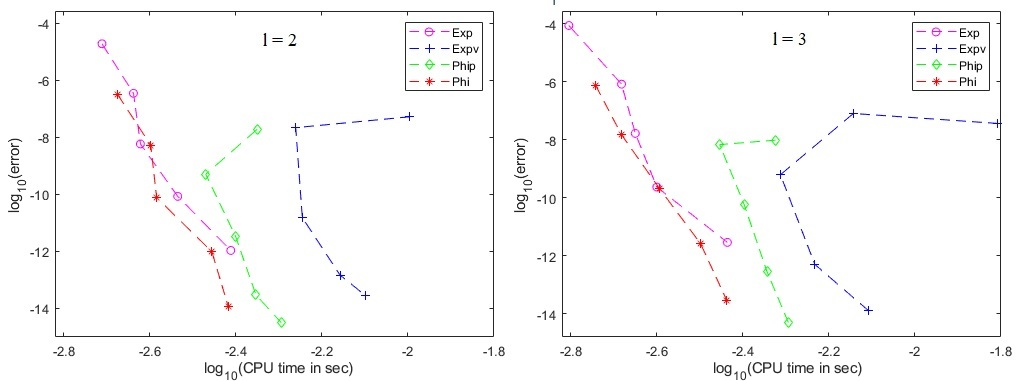
\includegraphics[scale=0.55]{Graphics/phil2l3.jpg}
	\caption{Diagrama tiempo-precisión para los métodos de \cite{hochbruck1997krylov}, \cite{sidje1998expokit}, \cite{niesen2012algorithm} y (\ref{phi_approx}), denotados por \textit{Exp}, \textit{Expv}, \textit{Phip} y \textit{Phi} respectivamente, como función de la dimensión de Krylov $\mf$, en el cálculo de  (\ref{sum2_phiXv}) para dos valores de $l$. Izquierda $l=2$, Derecha $l=3$. De arriba hacia debajo, $\mf=4,5,6,7,8$ para cada método, siendo $\mf=6$ el valor óptimo estimado como se especificó anteriormente con tolerancias $ATol=10^{-9}$ y $RTol=10^{-6}$.}
	\label{fig:SumPhi}
\end{figure}

\subsubsection{Simulaciones numéricas para Aproximaciones Krylov-Padé libre de Jacobiano}
Consideraremos el cálculo de (\ref{sum2_phiXv}) con matriz Jacobiana $f_x$ y campo vectorial $f$ del PVI resultante de discretizar una ecuación diferencial parcial. La siguiente matriz Jacobiana y la ecuación discretizada fue tomada de~\cite{tokman2006efficient}.

\begin{example}
	\label{ej:ej1-hpfj} Matriz Jacobiana de $2N\times2N$
	\begin{equation*}
	f_{x}(x)=\left[ 
	\begin{array}{cc}
	diag(2u\cdot v-4) & diag(u\cdot u) \\ 
	diag(3-2u\cdot v) & -diag(u\cdot u)%
	\end{array}%
	\right] +\frac{\alpha }{(\Delta z)^{2}}\left[ 
	\begin{array}{cc}
	K & 0 \\ 
	0 & K%
	\end{array}%
	\right] ,\text{ \ \ \ con \ \ \ \ }x=\left[ 
	\begin{array}{c}
	u \\ 
	v%
	\end{array}%
	\right] ,
	\end{equation*}
	\[
	K=\left[ 
	\begin{array}{ccccc}
	-2 & 1 &  &  & \\
	1 & -2 & 1 &  &  \\
	& \ddots  & \ddots  & \ddots  &  \\
	&  & 1 & -2 & 1 \\
	&  &  & 1 & -2%
	\end{array}%
	\right]_{N\times N}
	\]
	de la  ecuación $2N$-dimensional Brusselator discretizada
	\begin{eqnarray*}
		\frac{du_{i}}{dt} &=&1+u_{i}^{2}v_{i}-4u_{i}+\frac{\alpha }{(\Delta z)^{2}}%
		(u_{i-1}-2u_{i}+u_{i+1}) \\
		\frac{dv_{i}}{dt} &=&3u_{i}-u_{i}^{2}v_{i}+\frac{\alpha }{(\Delta z)^{2}}%
		(v_{i-1}-2v_{i}+v_{i+1})
	\end{eqnarray*}
	con $\alpha =1/50$, $u_{i}(0)=1+\sin (2\pi z_{i})$, $v_{i}(0)=3$, $z_{i}=i/(N+1)$, $\Delta z =1/(N+1)$, $i=1,\ldots,N$, y $N=800$.
\end{example}

Los códigos de Matlab \textit{JF1-Phi} y \textit{JF2-Phi} implementan la aproximación Krylov-Padé libre de Jacobiano (\ref{phi_approx_fj}) con $\beta=0$ y las diferencias finitas de primer y segundo orden respectivamente
\begin{equation}\label{finite-differences}
	g(x,u;\delta)=\frac{f(x+\delta u)-f(x)}{\delta}  \;\;\; \text{y} \;\;\; g(x,u;\delta)=\frac{f(x+\delta u)-f(x-\delta u)}{2\delta}
\end{equation}
donde $\delta= \frac{\sqrt{(1+||x||_2)\epsilon_{mach}}}{\epsilon_{mach}+||u||_2}$ como se sugiere en~\cite{knoll2004jacobian}, siendo $\epsilon_{mach}$ el épsilon de la máquina. El código de Matlab \textit{Phi} implementa la aproximación Krylov-Padé (\ref{phi_approx}) con la matriz exacta.

En el ejemplo, la matriz y los vectores en (\ref{sum2_phiXv}) se definen como $A=f_x(x(0))$, $a_1=a_2=f(x(0))$, $a_3=2a_1 $ y $a_4=6a_1$ de acuerdo con el número de términos $l$ en cada ejemplo. La norma euclidiana se usa para medir el error entre el valor ``exacto'' de $L e^{h M}r$ en (\ref{sum2_phiXv}) y sus aproximaciones. Para fines comparativos, el valor ``exacto'' de $e^{h M}$ y la matriz exponencial $\me{\tau\overline{H}}$ en los códigos \textit{JF1-Phi}, \textit{JF2-Phi} y \textit{Phi} se calculan con la misma función de Matlab \textit{expm}. La fila superior de la Figura \ref{fig:SumPhiBrusselator} presenta, para cada ejemplo, las gráficas logarítmicas de tolerancia relativa (\textit{rtol}) contra error (\textit{error}) en el cálculo de (\ref{sum2_phiXv}) mediante las aproximaciones \textit{JF1-Phi}, \textit{JF2-Phi} y \textit{Phi} con tolerancias relativas y absolutas $rtol=10^{-j}$ y $atol=0.1 rtol$, con $j=1,\ldots,6$. La fila inferior de esta figura presenta las gráficas de la dimensión de Krylov $\mf$ contra $log(rtol)$ correspondientes a las aproximaciones en la fila superior de las figuras. Los valores de $\mf$ son determinados automáticamente por cada código para cada una de las tolerancias especificadas $rtol$ y $atol$, tal y como se explicó anteriormente.

\begin{figure}[htb]
	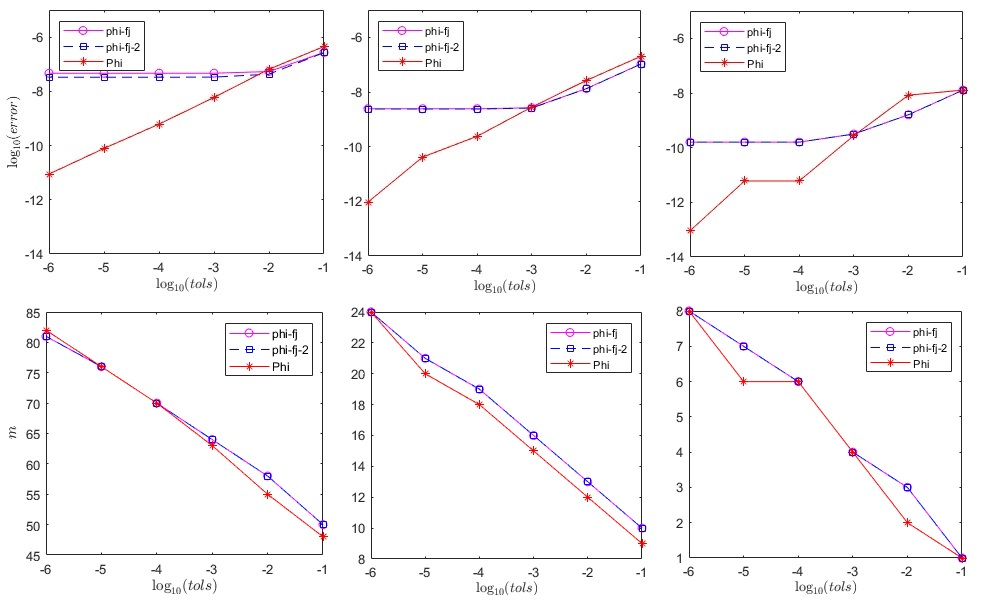
\includegraphics[scale=0.57]{Graphics/kpfj-brusselator-em.jpg}
	\caption{Superior: Gráficos Log-log de tolerancia relativa (\textit{rtol}) contra error (\textit{error}) en el cálculo de $\phi _{1}(f_x,h)a_{1}+\phi _{2}(f_x,h)a_{3}+\phi _{3}(f_x,h)a_{3}$ para la ecuación de ejemplo \ref{ej:ej1-hpfj} mediante las aproximaciones \textit{JF1-Phi}, \textit{JF2-Phi} y \textit{Phi} con $rtol=10^{-j}$ y $j=1,\ldots,6$. De izquierda a derecha, con $h=0.01,0.001,0.0001$. Inferior: Gráficos de tolerancia relativa (\textit{rtol}) contra dimensión de Krylov $\mf$ correspondiente a las aproximaciones de la figura superior.}
	\label{fig:SumPhiBrusselator}
\end{figure}

Observe que una diferencia importante entre las aproximaciones libre de Jacobiano y las de matriz exacta es el umbral para los errores de las primeras a medida que disminuye la tolerancia. Como es de esperar, cuando la tolerancia $rtol$ disminuye, la dimensión de Krylov $\mf$ para las tres aproximaciones aumenta y, en consecuencia, sus errores también disminuyen. Sin embargo, para valores crecientes de $\mf$, el valor fijo del segundo término de la derecha en (\ref{phi_approx_fj}) domina los valores decrecientes del primer término, lo que explica los umbrales para los errores de las aproximaciones libres de Jacobiano \textit{JF1-Phi} y \textit{JF2-Phi} en la Figura \ref{fig:SumPhiBrusselator}. Como se predice en (\ref{phi_approx}), el error de la aproximación con Jacobiano exacto \textit{Phi} en esta figura siempre disminuye cuando $\mf$ aumenta. Nótese también que, en correspondencia con el segundo término de la cota (\ref{phi_approx_fj}), la precisión de la aproximación con diferencia finita de segundo orden \textit{JF2-Phi} es ligeramente superior a la de la aproximación con diferencia finita de primer orden \textit{JF1-Phi} solo para los valores grandes de $h$ (gráfico superior izquierdo en la figura).

Las simulaciones numéricas corroboraron las principales implicaciones del análisis de errores para dicha aproximación libre de Jacobiano, es decir; el umbral para los errores disminuye cuando aumenta la dimensión del subespacio de Krylov; es menor el error de la aproximación con diferencia finita de segundo orden y  las aproximaciones libres de Jacobiano son menos precisas que las que utilizan matriz exacta.
\chapter{Método Runge-Kutta de Dormand y Prince Localmente Linealizado}\label{chapter:lldp}

En el Capítulo \ref{chapter:exp-int-and-ll-methods} se presentó la Aproximación Lineal Local de Orden Superior para EDO. Como se explicó en ese capítulo, a esa clase de métodos pertenecen los integradores numéricos derivados de dividir, en intervalos de tiempo consecutivos, la solución $x$ de la ecuación original en dos partes: la solución u de la ecuación linealizada localmente más una solución aproximada a la representación diferencial del residuo $r=x-u$ proporcionada por un integrador numérico de alto orden. En el Capítulo \ref{chapter:solve-non-smal-lineal-eq} se propusieron y utilizaron las aproximaciones Krylov-Padé para resolver la ecuación diferencial lineal de dimensiones no pequeñas. En éste capítulo se utilizará las fórmulas  Runge-Kutta embebidas de Dormand y Prince para aproximar la solución de la ecuación diferencial no lineal del residuo. Combinando estas aproximaciones se obtendrá el Método Runge-Kutta de Dormand y Prince Localmente Linealizado para EDOs de dimensiones no pequeñas. Utilizando las nuevas fórmulas, se construyen también estrategias adaptativas para implementar esquemas con tamaño de paso fijo y dimensión de Krylov variable, y esquemas con tamaño de paso y dimensión de Krylov variable. Los resultados de este capiítulo están basados en \cite{naranjo2021locally}.

Sin pérdida de generalidad consideremos el PVI autónomo $d$-dimensional
\begin{equation}\label{syst}
\frac{dx}{dt}=f(x), \; t\in[t_0,T],\end{equation}
\begin{equation}\label{systcond}
x(t_0)=x_0,
\end{equation}donde $f$ es una función diferenciable en una vecindad
$\mathfrak{D}$ del conjunto $\{x(t):t\in [t_0,T]\}$ de $\mathbb{R}^{d}$. Se asumen condiciones de Lipschitz y suavidad en la función $f$ para asegurar una solución única de esta ecuación en $\mathfrak{D}$.

\section{Fórmulas embebidas}

Sea $\left( t\right) _{h}=\left\{ t_{n}:n=0,1,\ldots ,N\right\}$ una discretización temporal con un tamaño de paso máximo $h$ definido como una secuencia de tiempos que satisfacen las condiciones $t_{0}<t_{1}<\cdots <t_{N}=T$, donde $h_{n}=t_{n+1}-t_{n}\leq h$ para $n=0,\ldots,N-1$.

Consideremos las fórmulas de Runge-Kutta localmente linealizadas de Dormand y Prince
\begin{equation} \label{lldis}
    z_{n+1}\,=\,z_n+u_s+h_n \sum_{j=1}^{s}b_j \kt_j \,\,\, \text{y} \,\,\, \
    \widehat{z}_{n+1}\,=\, z_n+u_s+h_n \sum_{j=1}^{s}\widehat{b}_j \kt_j
\end{equation}
introducidas en \cite{Jimenez14AMC} para aproximar la solución $x$ de (\ref{syst})-(\ref{systcond}) en $t_{n+1}$, para $n=0,\ldots,N -1$, donde s = 7 es el número de etapas,
\begin{equation*}
u_j=L\me{c_j M_n h_n}r,
\end{equation*}
\begin{equation*}
\kt_j = f\left( z_n+u_j+h_n \sum_{i=1}^{j-1}a_{j,i}\kt_i \right) - f( z_n) - f_x(z_n)u_j,
\end{equation*}
con $\kt_1 \equiv 0$, siendo $f_x$ la matriz Jacobiana de $f$ y $a_{j,i}$, $b_j$, $\widehat{b}_j$ los coeficientes de Runge-Kutta de Dormand y Príncipe definido en la Tabla \ref{ButcherTabla}. Aquí,
\begin{equation*}
    M_{n}=\left[
    \begin{array}{cc}
        f_{x}(z_{n}) & f(z_{n}) \\
        0_{1\times d} & 0
    \end{array}
    \right] \in \mathbb{R}^{(d+1)\times (d+1)},
\end{equation*}
$ L=[I_d \;\; 0_{d\times 1}] $ y $r=[0_{1\times d}\;\; 1]^T$. Como se mencionó en el Capítulo \ref{chapter:exp-int-and-ll-methods}, las fórmulas embebidas (\ref{lldis}) son instancias particulares de la clase general de Métodos de Linealización Local de Orden Superior propuestos en \cite{Jimenez13} y, con la aproximación de Padé para las exponenciales matriciales en $u_j$, fueron utilizadas en \cite{Jimenez14AMC} para integrar EDO de dimensiones pequeñas.

A continuación, para EDO de dimensiones no pequeñas, las aproximaciones Krylov-Padé propuestas en el capítulo anterior serán utilizadas para aproximar los términos $u_j$ que aparecen en (\ref{lldis}). Además, para aproximar eficientemente los cinco términos $u_j$ correspondientes a los cinco únicos $c_j$ distintos de cero que según la Tabla \ref{ButcherTabla} aparecen en las fórmulas (\ref{lldis}), se utilizará combinación conveniente de la invarianza ante escalado de la base ortonormal de los subespacios de Krylov, la propiedad de flujo del operador exponencial y el Teorema 1 en~\cite{sidje1998expokit}. De hecho, con la matriz de Hessenberg superior $H^*_\mf$ resultante del Algoritmo \ref{alg:Arnoldi} para $\mathcal{K}_\mf(h_nf_x,f)$, se obtiene la matriz de Hessenberg $H_\mf=H^*_\mf/h_n$ correspondiente a $\mathcal{K}_\mf(f_x,f)$, por lo que la exponencial de la matriz particionada
\begin{equation}
    \overline{H} = \left[\begin{array}{cccc}
    H_\mf & e_1 & 0_{\mf\times 1} & 0_{\mf\times 1}\\
    0_{1\times\mf} & 0 & 1 & 0\\
    0_{1\times\mf} & 0 & 0 & 1\\
    0_{1\times\mf} & 0 & 0 & 0
    \end{array}\right] \label{hhat}
\end{equation}
es calculada obteniéndose
\begin{equation}
    \me{\tau\overline{H}} = \left[\begin{array}{cccc}
    \me{\tau H_m} & \tau\phi_1(\tau H_m)e_1 & \tau^{2}\phi_2(\tau H_m)e_1 &
    \tau^{3}\phi_3(\tau H_m)e_1 \\
    & 1 & \tau & \frac{\tau^{2}}{2}\\
    &  & 1 & \tau \\
    &   &   & 1 \\
    \end{array}\right]\;. \label{phi_hhat}
\end{equation}
En particular, con $\gamma=\frac{1}{90}$, se calculada la matriz particionada $E_\gamma=\me{\gamma h_n\overline{H}}$, siendo $\frac{1}{ 90}$ el máximo común divisor de los coeficientes de Runge-Kutta $\frac{1}{5},\frac{3}{10},\frac{4}{5},\frac{8}{9} ,1$ de la Tabla \ref{ButcherTabla}. Entonces, usando la propiedad de flujo del operador exponencial, se obtiene
\begin{align}
    E_{2/90}& =E_{1/90}E_{1/90} & E_{4/90}& =E_{2/90}E_{2/90}  \notag \\
    E_{8/90}& =E_{4/90}E_{4/90} & E_{16/90}& =E_{8/90}E_{8/90}  \notag \\
    E_{32/90}& =E_{16/90}E_{16/90} & E_{80/90}& =E_{32/90}E_{16/90}E_{32/90}
    \label{flow} \\
    E_{1/10}& =E_{8/90}E_{1/90} & E_{1/5}& =E_{1/10}E_{1/10}  \notag \\
    E_{2/5}& =E_{1/5}E_{1/5} & E_{4/5}& =E_{2/5}E_{2/5}  \notag \\
    E_{3/10}& =E_{1/10}E_{1/5} & E_{1}& =E_{4/5}E_{1/5}\;,  \notag
\end{align}
con lo cual las cinco matrices requeridas $E_{c_j}$ son obtenidas. Como, en general, la exponencial de una matriz no puede ser calculada de forma exacta, $E_{1/90}=e^{\frac{h_n}{90}\overline{H}}$ es aproximada por 
\[\widetilde{E}_{h_n/90} = F_k^{\pf,\qf}\left(\frac{h_n}{90}\overline{H}\right), \]
donde $F_k^{\pf,\qf}(A)=(P_{\pf,\qf}(2^{-k}A))^{2^k}$ denota a la aproximación de Padé de $e^A$ con escalamiento y potenciación tal y como se explica en el Capítulo \ref{chapter:exp-int-and-ll-methods}

Consecuentemente, utilizando la aproximación Krylov-Padé (\ref{eq:kp_aprox}) y las expresiones (\ref{flow}) obtenemos las siguientes aproximaciones para cada $u_j$
\begin{eqnarray}
    \frac{1}{5}h_n\varphi_1\left(\frac{1}{5}h_n f_x\right)f & \approx & \beta   V_{\mf}\; [\widetilde{E}_{\frac{1}{5}}]_{12}\;  + \beta \hf_{\mf+1,\mf}e_\mf^T\; [\widetilde{E}_{\frac{1}{5}}]_{13}\;  v_{\mf+1} \notag \\
    \frac{3}{10}h_n\varphi_1\left(\frac{3}{10}h_n f_x\right)f & \approx & \beta   V_{\mf}\; [\widetilde{E}_{\frac{3}{10}}]_{12}\;  + \beta \hf_{\mf+1,\mf}e_\mf^T\; [\widetilde{E}_{\frac{3}{10}}]_{13}\;  v_{\mf+1} \notag \\
    \frac{4}{5}h_n\varphi_1\left(\frac{4}{5}h_n f_x\right)f & \approx & \beta   V_{\mf}\; [\widetilde{E}_{\frac{4}{5}}]_{12}\;  + \beta \hf_{\mf+1,\mf}e_\mf^T\; [\widetilde{E}_{\frac{4}{5}}]_{13}\;  v_{\mf+1} \label{phi_appox} \\
    \frac{8}{9}h_n\varphi_1\left(\frac{8}{9}h_n f_x\right)f & \approx & \beta   V_{\mf}\; [\widetilde{E}_{\frac{8}{9}}]_{12}\;  + \beta \hf_{\mf+1,\mf}e_\mf^T\; [\widetilde{E}_{\frac{8}{9}}]_{13}\;  v_{\mf+1} \notag \\
    h_n\varphi_1(h_n f_x)f & \approx &  \beta V_{\mf}\; [\widetilde{E}_1]_{12}\;  + \beta\hf_{\mf+1,\mf}e_\mf^T\; [\widetilde{E}_1]_{13}\;  v_{\mf+1}, \notag
\end{eqnarray}
donde $[\widetilde{E}_{c_j}]_{ik}$ denota la sub-matriz $i,k$ de la matriz particionada $\widetilde{E}_{c_j}$, $V_m$ es la matriz con base ortonormal de $\mathcal{K}_ \mf(f_x,f)$ ya calculado por el Algoritmo \ref{alg:Arnoldi} para $\mathcal{K}_\mf(h_nf_x,f)$, y $\beta=\nnorm{\nnorm{f} }_2$.

Utilizando la aproximación $(\mf , \pf ,\qf , k)$-Krylov-Padé (\ref{phi_appox}) para cada $u_j$ en las fórmulas embebidas (\ref{lldis}), obtenemos la Fórmulas de Runge-Kutta linealizadas localmente
\begin{equation}  \label{LLDPK scheme}
    y_{n+1}\,=\,y_n+\widetilde{u}_s+h_n \sum_{j=1}^{s}b_j \widetilde{\kt}_j \,\,\, \text{y} \,\,\, \
    \widehat{y}_{n+1}\,=\, y_n+\widetilde{u}_s+h_n \sum_{j=1}^{s}\widehat{b}_j \widetilde{\kt}_j,
\end{equation}
para integrar PVI de grandes dimensiones, donde
\begin{equation*}
    \widetilde{\kt}_j = f\left( y_n+\widetilde{u}_j+h_n \sum_{i=1}^{j-1}a_{j,i}\widetilde{\kt}_i \right) - f( y_n) - f_x(y_n)\widetilde{u}_j.
\end{equation*}
y $\widetilde{\kt}_1=0$, son $a_{j,i}$, $b_j$, $\widehat{b}_j$ los coeficientes de Runge-Kutta de  Dormand y Prince definidos en la Tabla \ref{ButcherTabla}.

Es importante destacar que, a diferencia de otros integradores exponenciales de alto orden, las fórmulas embebidas (\ref{LLDPK scheme}) involucran la aproximación de un solo producto de función phi por vector. En efecto, mientras que los integradores exponenciales en general requieren de aproximar varios términos de la forma $\tau^k \varphi_k(\tau A_k)b_k$ con más de un valor de $k$, las fórmulas embebidas (\ref{LLDPK scheme}) solo requieren la aproximación de la acción de una sola función phi sobre un único vector $\tau \varphi_1(\tau A_1)b_1$. Como se ha explicado anteriormente, las cinco aproximaciones $\widetilde{u}_j$ a los términos distintos de cero $c_jh_n\varphi_1(c_jh_nf_x)f$ que aparecen en (\ref{LLDPK scheme}) se calculan eficientemente en cada paso de integración por medio de solo una aproximación por un subespacio de Krylov que se construye mediante el algoritmo \ref{alg:Arnoldi} y solo una exponencial matricial mediante el método de Padé.

El siguiente teorema trata sobre la velocidad de convergencia de las fórmulas embebidas (\ref{LLDPK scheme}). Con este propósito, estas fórmulas se reescriben como
\begin{equation*}
    y_{n+1}=y_{n}+\digamma (y_{n};h_{n})\text{ \ \ \ \ y \ \ \ \ }\widehat{y}_{n+1}=y_{n}+\widehat{\digamma }(y_{n};h_{n}).
\end{equation*}


\begin{theorem}\label{theorem:lldp-convergence}
	\cite{naranjo2021locally}~Se $x$ solución del PVI (\ref{syst})-(\ref{systcond}) con campo vectorial $f$ seis veces continuamente diferenciable en con conjunto compacto $\mathfrak{K} \subset \mathfrak{D}$. Entonce, las formular Runge-Kutta Localmente Linealizadas (\ref{LLDPK scheme}) tienen error de truncamiento local
	\[\lvert\lvert x(t_{n+1}) - x(t_n) - \digamma(x(t_n);h_n) \rvert\rvert_2 \leq Kh_n^{\mathrm{min}\left\{ \mf+2,\pf+\qf+1 \right\}}+C h_n^{6}  \]
	\[\lvert\lvert x(t_{n+1}) - x(t_n) - \widehat{\digamma }(x(t_n);h_n) \rvert\rvert_2 \leq Kh_n^{\mathrm{min}\left\{ \mf+2,\pf+\qf+1 \right\}}+C h_n^{5}  \]
	y erro global
	\[ \lvert\lvert x(t_{n+1}) - y_{n+1} \rvert\rvert_2 \leq M h^{\mathrm{min}\left\{5,\mf+1,\pf+\qf \right\}} \]
	\[ \lvert\lvert x(t_{n+1}) - \widehat{y}_{n+1} \rvert\rvert_2 \leq M h^{\mathrm{min}\left\{ 4,\mf+1,\pf+\qf \right\}} \]
	$\forall t_{n+1},t_n\in(t)_h$ y $h$ suficientemente pequeña, donde  $K,C,M$ son constantes positivas.
\end{theorem}
\emph{Demostración} Utilizando el Teorema~\ref{theorem:Krylov-bound}, se tiene
\begin{equation}\label{proof:ErrorLinearODE}
\nnorm{\nnorm{ u_j-K_{\mf,k}^{\pf,\qf}\left(c_j h_n,f_x , f \right) }}_2 =  \nnorm{\nnorm{c_jh_n\varphi_1(c_jh_nf_x)f - K_{\mf,k}^{\pf,\qf}\left(c_j h_n, f_x , f \right) }}_2 \le Kh_n^{\mathrm{min}\left\{ \mf+2,\pf+\qf+1 \right\}},
\end{equation}
con $j=1,\ldots,7$, donde $K$ es una constante positiva. Dado que $z_{n+1} = y_n + u_7$ es la solución exacta de la EDO lineal $dz/dt=f(y_n)+f_x(y_n)(z-y_n)$ resultante de la linealización local de la ecuación~(\ref{syst}) en $t_n$ con la condición inicial $z(t_n)=y_n$ y los errores de truncamiento local de las fórmulas embebidas de Runge-Kutta de Dormand y Prince son 6 y 5, los errores de truncamiento local y global del Las fórmulas de Runge-Kutta localmente linealizadas (\ref{LLDPK scheme}) se derivan directamente del Teorema 15 en~\cite{Jimenez13} y (\ref{proof:ErrorLinearODE}). $\Box$\\

Claramente, según este resultado, las fórmulas embebidas Runge-Kutta localmente linealizadas (\ref{LLDPK scheme}) preservan la velocidad de convergencia de las fórmulas embebidas clásicas Runge-Kutta de Dormand y Prince si las desigualdades $\mf+1 \ge 5 $ y $\pf+\qf \ge 5$ se cumplen. Además, al igual que las fórmulas embebidas para pequeños PVI y otros integradores de tipo exponencial, las nuevas fórmulas embebidas (\ref{LLDPK scheme}) son capaces de integrar PVI lineales tan precisos como sea necesario independientemente de la dimensionalidad y \textit{stiffness} de las ecuaciones. Sin embargo, dado que, por construcción, las fórmulas (\ref{LLDPK scheme}) usan las fórmulas originales de Runge-Kutta de Dormand y Prince para resolver una ecuación auxiliar no lineal (ver detalles en \cite{Jimenez13, Jimenez14AMC}), las fórmulas (\ref{LLDPK scheme}) no están diseñadas para integrar PVI \textit{stiff} en general. De esta forma, las fórmulas propuestas (\ref{LLDPK scheme}) pretenden aproximar la solución de PVI grandes para los que la principal fuente de \textit{stiffness} surge de la linealización de la ecuación no lineal en consideración. Estos son precisamente la mayoría de los grandes PVI resultantes de la discretización espacial de las EDP que modelan procesos físicos, biofísicos y físico-químicos conocidos.
\begin{table}[h]
	\caption{ Valores de los coeficientes $\alpha _{i,j}$ en las fórmulas continuas (\ref{continuousLLRK45})\label{Table continuous RK}}
	\centering
	\begin{tabular}{ccccc}
		\hline
		$j\setminus i$ & $1$ & $2$ & $3$ & $4$ \\
		\hline
		$1$ & $1$ & $-183/64$ & $37/12$ & $-145/128$ \\
		$2$ & $0$ & $0$ & $0$ & $0$ \\
		$3$ & $0$ & $1500/371$ & $-1000/159$ & $1000/371$ \\
		$4$ & $0$ & $-125/32$ & $125/12$ & $-375/64$ \\
		$5$ & $0$ &	$9477/3392$ & $-729/106$ & $25515/6784$ \\
		$6$ & $0$ &	$-11/7$ & $11/3$ & $-55/28$ \\
		$7$ & $0$ & $3/2$ & $-4$ & $5/2$ \\
		\hline
	\end{tabular}
\end{table}

Cuando se requiere la solución en un conjunto denso de instantes de tiempo entre dos pasos de integración consecutivos, normalmente se utilizan fórmulas continuas para proceder con un costo computacional mínimo (consulte, por ejemplo, la Sección II.6 en \cite{hairer1993solving}). Regularmente, estas fórmulas continuas se construyen mediante una interpolación polinomial de las fórmulas de integración entre dos pasos de integración consecutivos $t_{n},t_{n+1}\in $ $ t_{h}$. Mediante una simple combinación de las fórmulas embebidas (\ref{LLDPK scheme}) con las fórmulas continuas de Runge-Kutta de Dormand y Prince dadas en \cite{hairer1993solving}, se obtiene la siguiente fórmula continua de $7$ etapas
\begin{equation}
    y(t_{n}+\theta h_{n})=y_n+\widetilde{u}(\theta
    h_{n})+h_{n}\sum_{j=1}^{7}b_{j}(t_{n}+\theta h_{n})\widetilde{\kt}_{j}\
    ,\ \ 0<\theta <1,  \label{continuousLLRK45}
\end{equation}%
 para todo $t_{n} \in $ $\left( t\right) _{h}$, donde
\begin{equation*}
    \widetilde{u}(\theta h_{n}) = K_{\mf,k}^{\pf,\qf}\left(h_n\theta, f_x , f \right)
\end{equation*}
    es el vector $d$-dimensional,
\begin{equation*}
    b_{j}(\delta )=\sum\limits_{i=1}^{4}\alpha _{i,j}\delta ^{i}
\end{equation*}
es un polinomio con coeficientes $\alpha _{i,j}$, y la función $\widetilde{\kt}_{j}$ se define como en (\ref{LLDPK scheme}). Los coeficientes $\alpha _{i,j}$, definidos en
Tabla \ref{Table continuous RK}, coinciden con las de la
fórmula continua de Runge-Kutta implementada en el código de Matlab ode$45$. Para la fórmula continua (\ref{continuousLLRK45}) se pueden definir dos salidas densas convenientes. La primera, de 4 elementos, incluye los pares $(t_{n}+\theta h_{n},y(t_{n}+\theta h_{n}))$ correspondientes a los cuatro $\theta = c_j $, con $0<c_j<1$, para la cual ya se han calculado las aproximaciones $\widetilde{u}_j$ en (\ref{LLDPK scheme}). El segundo conjunto se define con los doce valores
$\{\frac{1}{90},\frac{2}{90},\frac{4}{90},\frac{8}{90},\frac{1}{10},\frac {16}{90},c_2,c_3,\frac{32}{90},\frac{2}{5},c_4,c_5\}$ de $\theta$ para las cuales las matrices $E_\theta$ en (\ref{flow}) fueron calculados. En este caso, $\widetilde{u}(\theta h_{n})$ debe evaluarse en los ocho valores de $\theta \ne c_j$, pero sin requerir alguna nueva aproximación del subespacio de Krylov.

Antes de concluir esta sección, es importante destacar que las fórmulas embebidas (\ref{LLDPK scheme}) como implementación numérica de las fórmulas embebidas (\ref{lldis}) también pertenecen a la clase general de Métodos de Linealización Local de Orden Superior de \cite{Jimenez13}. Además, téngase en cuenta que, simplemente reemplazando en (\ref{LLDPK scheme}) los coeficientes de la Tabla \ref{ButcherTabla} por otros correspondientes a un par diferente de fórmulas de Runge-Kutta explícitas embebidas con $s$ estados, un nuevo par de formulas embebidas Runge-Kutta linealizadas localmente se obtienen directamente para IVP de grandes dimensiones. La velocidad de convergencia de tales nuevas fórmulas se obtiene, como en la demostración del Teorema \ref{theorem:lldp-convergence}, simplemente combinando el Teorema 15 en~\cite{Jimenez13} y el Teorema \ref{theorem:Krylov-bound}. Además, si los coeficientes de Runge-Kutta $c_i$ de las nuevas fórmulas admiten un máximo común divisor $\gamma$ entonces, un procedimiento similar al descrito en (\ref{flow}) puede seguirse para calcular los diferentes términos $u_j$ de manera eficiente.

\section{Esquemas con tamaño de paso fijo y dimensión de Krylov variable}\label{section:lldp-fix-step}

Las nuevas fórmulas embebidas (\ref{LLDPK scheme}) introducidas en la sección anterior para integrar PVI de grandes dimensiones
dependen de valores no especificados para la dimensión Krylov $\mf$ y el orden Padé $(\pf ,\qf)$. En esta sección se propone una estrategia adaptativa para la estimación de valores adecuados para $\mf, \pf ,\qf$ en fórmulas (\ref{LLDPK scheme}) en cada paso de integración en una partición de tiempo uniforme.

\subsection{Selección de la dimensión de Krylov}\label{sec:selkrydim}

Similar al error relativo utilizado en la Sección \ref{section:num-sim-kp}, el error relativo en la aproximación \ref{LLDPK scheme} para $u_j$ está dado por
\begin{equation}
    \varepsilon_{K} = \left(\frac{1}{d}\sum\limits_{i=1}^{d} \left(\frac{\beta
        \hf_{\mf+1,\mf} e_{\mf}^T
        [\widetilde{E}_\mathfrak{c}]_{14} \rho^{[i]}}{ATol+ RTol\cdotp
        \rvert y_{n}^{[i]}\rvert}\right)^{2}\right)^{1/2},
    \label{errrel}
\end{equation}
donde $ATol$ y $RTol$ son las tolerancias absoluta y Relativa, $\mathfrak{c}=\maxx{c_j}$, $\rho = f_x v_{\mf+1}$ y $\beta=\nnorm{\nnorm{f}}_2$.

Después de la construcción de la base ortonormal del $\mf$-ésimo subespacio Krylov $\mathcal{K}_\mf(f_x,f)$, son posibles dos alternativas: $\varepsilon_{K}/\gamma_{K}< 1$ o al contrario, donde $\varepsilon_{K}$
es el error relativo~(\ref{errrel}) y $\gamma_{K}=0.005$ es un factor de seguridad.

En el caso de $\varepsilon_{K}/\gamma_{K}< 1$, se acepta la aproximación (\ref{phi_appox}) para $u_j$ y la nueva dimensión del subespacio de Krylov $\mathfrak{m}_{new}$ que se utilizará en el siguiente paso de integración se calcula mediante la fórmula
\begin{equation}\label{calcmnew}
    \mathfrak{m}_{new}= \maxx{\mf_{min}, \minn{\mf , \mf_{max} }},
\end{equation}
    donde $\mf_{min}$ y $\mf_{max}$ son los valores máximo y mínimo posibles para la dimensión del Krylov,
\begin{equation*}
    \mf = \left\lfloor \mf_{n} + \maxx{\fac_{max} , \minn{\fac_{min},
            \fac\cdot\Delta\mf} } \right\rfloor,
\end{equation*}
\begin{equation}
    \Delta\mf=\log(\varepsilon_{K}/\gamma_{K}) \label{delta_m}
\end{equation}
$\fac_{max}= -\frac{\mf_n}{4}$, $\fac_{min}= \frac{\mf_n}{3}$, $\fac=\frac{1}{\log( 2)}$, y $\left\lfloor \cdot \right\rfloor$ denota la función suelo(que devuelve el mayor entero menor o igual que un número real dado). De lo contrario, se rechaza la aproximación (\ref{phi_appox}) para $u_j$ para el $\mf_n$ dado y se estima un nuevo valor para la dimensión del subespacio de Krylov $\mf_{new}$ mediante (\ref{calcmnew}), pero con $\mf$ calculado por la expresión
\begin{equation*}
    \mf = \left\lceil \mf_{n} + \minn{\fac_{max} , \maxx{\fac_{min},
            \fac\cdot\Delta\mf} } \right\rceil,
\end{equation*}
donde $\fac_{max}= \maxx{ 1,\frac{\mf_{n}}{3} }$, $\fac_{min}= 1 $, $\fac=\frac{1}{\log (2)}$, y $\left\lceil \cdot \right\rceil$ denota la función techo(que devuelve el menor entero mayor o igual que un número real dado). Los vectores ortonormales extra $\{v_{\mf+1},\ldots,v_{\mf_{new}} \}$ correspondientes al $\mf_{new}$-ésimo subespacio de Krylov $\mathcal{K}_{\mf_{new}}(f_x,f)$ son calculados a través del Algoritmo \ref{alg:Arnoldiexpand}.
\begin{algorithm}[h!]
	\caption{Algoritmo de Arnoldi para expandir la base ortonormal $\{v_1,\ldots,v_{\mf} \}$ del $\mf$-ésimo subespacio de Krylov $\mathcal{K}_{\mf}(A,b)=span\{b,Ab,\ldots,A^{\mf}b\}$ a la base ortonormal $\{v_1,\ldots,v_{\mf},\ldots,v_{\mf_{new}} \}$ del $\mf_{new}$-ésimo subespacio de Krylov ${\mathcal{K}_{\mf_{new}}(A,b)=span\{b,Ab,\ldots,A^{\mf_{new}}b\}}$}
    \label{alg:Arnoldiexpand}
	\KwIn{$A\in \mathbb{R}^{d\times d}$, $b\in \mathbb{R}^{d}$, $V_{\mf}\in \mathbb{R}^{d\times \mf}$, $H^*_{\mf}\in\mathbb{R}^{\mf\times \mf}$, $v_{\mf+1}\in \mathbb{R}^{d}$, $\hf_{\mf+1,\mf} \ge 0$, y la nueva dimensión $\mf_{new}$ del subespacio de Krylov}
	\KwOut{$V_{\mf_{new}}=[v_1\,\cdots \,v_{\mf_{new}}]\in \mathbb{R}^{d\times \mf_{new}}$, matriz de Hessenberg superior $H^*_{\mf_{new}}=V_\mf^{\intercal} A V_{\mf_{new}} $, $v_{\mf_{new}+1}$,  $\hf_{\mf_{new}+1}$, $\mf_{new}$, $\mf_{cut}$, $breakdown$}
	Líneas 3-17 en el Algoritmo \ref{alg:Arnoldi}, pero reemplazando la línea 3 por \textbf{for} $j=\mf+1,\ldots,\mf_{new}$ \textbf{do}
\end{algorithm}
El estimador propuesto (\ref{calcmnew}) para $\mf_{new}$ es un refinamiento del considerado en el Algoritmo 3 de \cite{niesen2012algorithm} orientado a reducir las fluctuaciones en la estimación de la dimensión de los subespacios de Krylov. Además, el valor de $\mf_{min}$ en (\ref{calcmnew}) debe ser tal que conserve la velocidad de convergencia de las fórmulas embebidas originales de Dormand y Prince como se establece en el Teorema \ref{theorem:lldp-convergence}.

\subsection{Selección del orden de Padé}\label{sec:pade-order}
Como se ha señalado en varios artículos (ver \cite{jimenez2009rate,jimenez2012convergence, Jimenez14AMC, jimenez2015convergence}), la selección de un valor apropiado del par $(\pf,\qf)$ en la aproximación del Padé es crucial para mejorar la eficiencia computacional de los integradores exponenciales. Para este propósito, la Tabla 1 en \cite{moler2003nineteen} se usa regularmente para configurar automáticamente los valores óptimos de $\pf$, con $\qf=\pf$, en función de la norma de la matriz, la tolerancia especificada y la orden de convergencia del integrador exponencial. La Tabla \ref{table:padep}, presenta un subconjunto de la mencionada Tabla 1 en \cite{moler2003nineteen} correspondiente a $\pf \ge 3$.

\begin{table}[htb]
	\caption{Valores óptimos de $\pf$ para las aproximaciones  (\ref{phi_approx},\ref{phi_approx_fj}), con $\qf=\pf$, como función de $\lvert\lvert \tau\overline{H} \rvert\rvert_\infty$ y la tolerancia deseada $\mathrm{RTol}$.}
	\begin{center}
		\begin{tabular}{cccc}
			\hline
			$\lvert\lvert \tau\overline{H} \rvert\rvert_\infty \setminus RTol$ & $10^{-9}$ & $10^{-12}$ & $10^{-15}$ \\
			\hline
			$<1$ & 3 & 4 & 4 \\
			$\geq 1$ & 4 & 5 & 6 \\
			\hline
		\end{tabular}
		\label{table:padep}
	\end{center}
\end{table}

\subsection{Esbozo del Esquema}

En los dos sub-secciones anteriores se propusieron procedimientos automáticos para la selección de la dimensión Krylov $\mf$ y el orden Padé $\pf$ en la aproximación Krylov-Padé (\ref{phi_appox}) para $u_j$. Al combinar estos procedimientos con las fórmulas (\ref{LLDPK scheme}), se pueden construir dos esquemas adaptativos con tamaño de paso fijo y dimensión de Krylov variable. Estos esquemas, de orden $r=4$ y $r=5$, están resumidos en Algoritmo~\ref{alg:integratorfix}.

{\SetAlgoNoLine
\begin{algorithm}[htb]
	\caption{Esquema de orden $r\,(=4,5)$ con tamaño de paso fijo y dimensión de Krylov variable}
	\label{alg:integratorfix}
	\KwIn{intervalo de tiempo $[t_0, T]$, valor inicial $y_0$, tamaño de paso $h$, dimensión máxima y mínima de los subespacios de Krylov $\mf_{max}$ y $\mf_{min}$, tolerancia absoluta y relative $Atol$ y $Rtol$}

	\KwOut{$\{y_0,\ldots,y_n\}$}
	$n=0$, $\mf_0=\mf_{min}$ \\
	\While{$t_n \le T$}{
		Ejecutar Algoritmo~\ref{alg:Arnoldi} para obtener matrices $H^*_{m_n}$ y $V_{m_n}$ de $\mathcal{K}_{\mf_n}(hf_x,f)$ y establecer valor $H_{m_n}=H^*_{m_n}/h_n$  \\
		Seleccionar orden de Padé $\pf$ según Sección~\ref{sec:pade-order} \\
		Estimar error relativo $\varepsilon_{K}$ mediante fórmula~(\ref{errrel}) \\
		\While{$\varepsilon_{K}/\gamma_{K} \geq 1$ y $\mf_n<\mf_{max}$}{
			Estimar nueva dimensión de Krylov $\mf_{new}$ mediante fórmula (\ref{calcmnew}) \\
			Ejecutar Algoritmo~\ref{alg:Arnoldiexpand} para obtener matrices $H^*_{m_{new}}$ y $V_{m_{new}}$ de $\mathcal{K}_{\mf_{new}}(hf_x,f)$ y establecer valor $H_{m_{new}}=H^*_{m_{new}}/h_n$ \\
			Establecer valor $\mf_n=\mf_{new}$ y actualizar todas las varibales que dependan de $\mf_n$ \\
            Seleccionar orden de Padé $\pf$ según Sección~\ref{sec:pade-order} \\
		    Estimar error relativo $\varepsilon_{K}$ mediante fórmula~(\ref{errrel}) \\
		}
     	Calcular $\widetilde{u}_j$ mediante fórmula (\ref{eq:kp_aprox})\\
        Evaluar la fórmula de order $r$ en (\ref{LLDPK scheme})~(i.e., $\widehat{y}_{n+1}$ or $y_{n+1}$) \\
	    Estimar nueva dimensión de Krylov $\mf_{new}$ mediante fórmula (\ref{calcmnew})\\
		$n=n+1$, $t_n=t_{n-1}+h$, $\mf_n=\mf_{new}$
	}
\end{algorithm}
}

\subsection{Ecuaciones de prueba}\label{section:test-eq}
En el marco de los integradores exponenciales, los seis modelos que se considerarán a continuación (y, también, en el próximo Capítulo) se han utilizado ampliamente en la literatura como ecuaciones de prueba. Véase, por ejemplo, \cite{tokman2006efficient,tokman2012new,tokman2013comparative} y los artículos incluidos. Como en \cite{tokman2006efficient,tokman2012new,tokman2013comparative}, estos modelos que involucran ecuaciones diferenciales parciales se discretizan espacialmente mediante el método de líneas para obtener grandes sistemas de IVP. Específicamente, siguiendo \cite{tokman2006efficient,tokman2012new,tokman2013comparative}, la primera y la segunda derivada parcial con respecto a las variables espaciales se discretizan con la diferencia finita centrada de segundo orden.

\begin{example}
    \label{ex:cusp} CUSP~\cite{wanner1996solving,tokman2006efficient}. Este sistema es una combinación del mecanismo de umbral del impulso nervioso de la ecuación de conducción nerviosa de Fitz-Hugh y Nagumo~\cite{fitzhugh1969mathematical,nagumo1962active}, la catástrofe de la cúspide ``con retorno suave''~\cite{zeeman1973differential} y el oscilador de Van der Pol
    \begin{eqnarray*}
        \frac{\partial y}{\partial t} &=& -\frac{y^{3}+ay+b}{\varepsilon}+\sigma\frac{\partial^{2}y}{\partial x^{2}}\\
        \frac{\partial a}{\partial t} &=& b+0\mathord{.}07v+\sigma \frac{\partial^{2}a}{\partial x^{2}}\\
        \frac{\partial b}{\partial t} &=& (1-a^{2})b-a-0\mathord{.}4y+0\mathord{.}035v+\sigma\frac{\partial^{2}b}{\partial x^{2}}
    \end{eqnarray*}
    en el intervalo de tiempo $t\in [0,10^{-4}]$, donde $\varepsilon=10^{-4}$, $\sigma=1/144$, y
    \[ v= \frac{u}{u+0\mathord{.}1},\;\; u=(y-0\mathord{.}7)(y-1\mathord{.}3).\]
    Estas ecuaciones se consideran en el dominio $0\leq x\leq 1$ y se discretizan como en \cite{tokman2006efficient} en una malla de $M$ puntos internos $x_i = i/M$ con espaciamiento $\Delta x=1/M$. Se imponen condiciones de contorno periódicas en $y,a,b$ y las condiciones iniciales se establecen en
    \[y(x, 0)=0,\;\;a(x, 0)=-\cos(2\pi x),\;\;b(x, 0)=2\sin(2\pi x).\]
    Los parámetros en estas ecuaciones se eligieron de tal manera que el \textit{stiffness} proviene tanto de la discretización espacial de los términos difusivos como del pequeño factor $\varepsilon$ que divide el término no lineal del lado derecho en la ecuación para $y$ .
\end{example}

\begin{example}\label{ex:Burgers}
     La ecuación de Burgers~\cite{tokman2006efficient} emergente en varias áreas de las matemáticas aplicadas, como la mecánica de fluidos, la acústica no lineal, la dinámica de gases y el flujo de tráfico
    \[ u_t+uu_x=\nu u_{xx} \]
    donde $\nu = 3\cdot10^{-4}$, $t\in [0,0\mathord{.}5]$ y $0\leq x\leq 1$, con condición inicial y valores de frontera
    \begin{equation*}
    u(0,t)=u(1,t)=0 \;\;\; ,   \;\;\;  u(x,0)=(\sin(3\pi x))^{2}(1-x)^{3/2}.
    \end{equation*}
    La ecuación se discretizó como en \cite{tokman2006efficient} en una malla de $M$ puntos internos $x_i = i/(M+1)$ con espaciado $\Delta x=1/(M+1)$, y el término $uu_x$ fue tomado como
    \[ \frac{u_{i+1}^{2}-u_{i-1}^{2}}{4\Delta x} \;\;\;\;  i=1,\ldots,M.\]
\end{example}

\begin{example}\label{ex:Brus2D}
    Ecuación 2D de Brusselator ~\cite{lefever1971chemical,tokman2012new} que modela las reacciones multimoleculares en el espacio bidimensional usando las leyes de la cinética química
    \begin{eqnarray*}
        \frac{\partial u}{\partial t} &=&1+uv^{2}-4u+\alpha \nabla^{2}u\\
        \frac{\partial v}{\partial t}&=&3u-u^{2}v+\alpha \nabla^{2}v,
    \end{eqnarray*}
    donde $\alpha = 0\mathord{.}02$, $t\in[0, 0\mathord{.}1]$ y $x,y\in[0,1]$,
    con condiciones de frontera de Newman y condiciones iniciales
    \begin{eqnarray*}
        u(x,y,0)=1+\sin(2\pi x)\sin(2\pi y) &,& v(x,y,0)=3.
    \end{eqnarray*}
    La discretización se realizó como en el código de \cite{jansing2011expode} sobre una malla de $M^2$ puntos internos.
\end{example}

\begin{example}\label{ex:Brus}
    Ecuación de Brusselator~\cite{lefever1971chemical,tokman2006efficient} que modela las reacciones multimoleculares utilizando las leyes de la cinética química
    \begin{eqnarray*}
        \frac{\partial u}{\partial t}&=&1+uv^{2}-4u+\alpha \frac{\partial ^{2}u}{\partial x^{2}}\\
        \frac{\partial v}{\partial t}&=&3u-u^{2}v+\alpha \frac{\partial ^{2}v}{\partial x^{2}},
    \end{eqnarray*}
    donde $\alpha = 0\mathord{.}02$, $t\in [0,1]$ y $0\leq x \leq 1$ con condiciones iniciales y de frontera
    \begin{eqnarray*}
        u(0,t)=u(1,t)=1 &,& v(0,t)=v(1,t)=3\\
        u(x,0)=1+\sin(2\pi x) &,& v(x,0)=3 .
    \end{eqnarray*}
    Del mismo modo, en \cite{tokman2006efficient}, los términos difusivos se discretizaron utilizando diferencias finitas centradas de segundo orden en la red espacial $x_i=\frac{i}{M+1}$ con espaciado  $\Delta x = \frac{1}{M+1}$ e $i=1,\ldots,M$.
\end{example}

\begin{example}\label{ex:GS2D}
    Ecuación 2D de Gray-Scott~\cite{gray1984autocatalytic,tokman2012new} que modela las reacciones autocatalíticas en el reactor de tanque agitado continuo e isotérmico
    \begin{eqnarray*}
        \frac{\partial u}{\partial t} &=& d_u\nabla^{2}u -uv^{2}+a(1-u) \\
        \frac{\partial v}{\partial t} &=& d_v\nabla^{2}v +uv^{2}-(a+b)v,
    \end{eqnarray*}
    donde $d_u=0\mathord{.}2,\,d_v=0\mathord{.}1,\,a=0\mathord{.}04,\,b=0\mathord{.}06$, $t\in[0, 0\mathord{.}1]$ y $x,y\in[0,1]$, con condiciones de frontera de Newman y condiciones iniciales
    \begin{eqnarray*}
        u(x,y,0) & = & 1-\me{-150\left(x-\frac{1}{2}\right)^{2}+\left(y-\frac{1}{2}\right)^{2}}\\
        v(x,y,0) & = & \me{-150\left(x-\frac{1}{2}\right)^{2}+2\left(y-\frac{1}{2}\right)^{2}}.
    \end{eqnarray*}
    La discretización se llevó a cabo como en el Ejemplo~\ref{ex:Brus2D}.
\end{example}

\begin{example}
    La ecuación DND (\emph{Degenerate Nonlinear Diffusion})~\cite{sherratt2010form,tokman2013comparative} es un modelo de reacción-difusión con difusión no lineal degenerada que se ha aplicado para describir la propagación de poblaciones en varios contextos biológicos, como la biología de células eucariotas y la formación de patrones en colonias bacterianas.
    \[ \frac{\partial u}{\partial t} = \frac{\partial}{\partial x}\left[ u\frac{\partial u}{\partial x} \right] + u(1-u), \]
    donde $t\in[0, 0\mathord{.}1]$ y $-23 < x < 50$, con condiciones de frontera $u(-23,t) = 1$, $u(50,t)=0$ y condiciones iniciales
    \[ u(x,0)=\begin{cases}
    1 & \text{if }x\leq 0\\
    \me{-0\mathord{.}8284x} & \text{if}x>0
    \end{cases}. \]
    La discretización se realizó sobre una malla de $M$ puntos internos $x_i=\frac{50*i}{M+1}-23\left(1-\frac{i}{M+1}\right)$ con $i=1,\ldots,M$.
\end{example}


\subsection{Experimentos numéricos}\label{section:num-exp-lldp-fix-step}
En la Sección \ref{section:lldp-fix-step}, se introdujeron las nuevas fórmulas embebidas (\ref{LLDPK scheme}) para integrar PVI de grandes. Además, se diseñó el algoritmo adaptativo \ref{alg:integratorfix} para estas fórmulas con tamaño de paso fijo. En esta sección, primero se estimará con simulaciones el orden de convergencia de las fórmulas embebidas (\ref{LLDPK scheme}) para ilustrar los resultados de convergencia establecidos en el Teorema \ref{theorem:lldp-convergence}. Posteriormente, también con simulaciones numéricas, se analizará el desempeño de los esquemas resumidos en el Algoritmo \ref{alg:integratorfix}. Esto incluirá la integración numérica de las ecuaciones de prueba de la sección anterior y una comparación con otros integradores exponenciales.

\subsubsection{Simulaciones preliminares}
En este primer conjunto de simulaciones, se evaluará el orden de convergencia de las fórmulas $y_n$ y $\widehat{y}_n$ definidas en (\ref{LLDPK scheme}) en función de la dimensión de Krylov $\mf$ y el orden de Padé $\pf$. Con ese propósito, los errores $e_i=\max_{t_n\in(t)_{h_i}}\nnnorm{y_n-x(t_n)}_\infty$ y $\widehat{e}_i=\max_{t_n\in(t )_{h_i}}\nnnorm{\widehat{y}_n-x(t_n)}_\infty$ en la integración del Ejemplo \ref{ex:Brus} con $M=100$ ($d=200$ ) se calcularon para cinco discretizaciones de tiempo diferentes $(t)_{h_i}$ con un tamaño de paso fijo $h_i$, donde la \textquotedblleft solución exacta\textquotedblright $x$ se estima mediante el código Matlab \textit{ode15s} con tolerancias $RTol=10^{ -12}$ y $ATol=10^{-14}$. La Figura \ref{fig:num-exp-lldp-fix-step:Fig3} muestra estos cinco errores para las fórmulas (\ref{LLDPK scheme}) con varios valores de m y $\pf=6$ fijos, así como la línea recta ajustada a los puntos $(\log_2( h_i),\log_2(e_i))$ y $(\log_2(h_i),\log_2(\widehat{e}_i))$ con $i=1,...,5$. La Tabla \ref{tab:num-exp-lldp-fix-step:morders} presenta el valor de la pendiente $\widetilde{r}$ de la recta ajustada para cada valor de $\mf$, lo que proporciona una estimación del orden de convergencia $r$ de cada esquema. La tabla también presenta los límites de confianza de $90\%$ de $\widetilde{r}$, el coeficiente de determinación como indicador de la bondad de la línea ajustada y el orden de convergencia esperado que, de acuerdo con el Teorema \ref{theorem:lldp-convergence}, las fórmulas (\ref{LLDPK scheme}) tienen para el $\mf$ dado. La Figura \ref{fig:num-exp-lldp-fix-step:Fig2} y la Tabla \ref{tab:num-exp-lldp-fix-step:porders} presentan salidas similares pero para las fórmulas (\ref{LLDPK scheme}) con $\mf=11$ fijo y varios valores de $\pf$. Se puede observar que el orden de convergencia estimado $\widetilde{r}$ proporcionada en las Tablas \ref{tab:num-exp-lldp-fix-step:morders} y \ref{tab:num-exp-lldp-fix-step:porders} está de acuerdo con el orden de convergencia de las fórmulas (\ref{LLDPK scheme}) indicados por el Teorema \ref{theorem:lldp-convergence} para los valores considerados de $\mf$ y $\pf$. Además, la Figura \ref{fig:num-exp-lldp-fix-step:Fig4} muestra los errores $e_i$ y $\widehat{e}_i$ de las fórmulas (\ref{LLDPK scheme}) con $\mf=11$ y $\pf=6$ fijos calculado para el tamaño de cinco pasos $h_i$ y la línea recta ajustada. En este caso, el orden de convergencia estimado $\widetilde{r}$ para las fórmulas $y_n$ y $\widehat{y}_n$ son $5.01 \pm 0.47$ y $3.93 \pm 0.19$ , respectivamente, lo cual concuerda con el índice global errores de discretización 5 y 4 dados en el Teorema \ref{theorem:lldp-convergence} para estas fórmulas.


\begin{figure}[h]
	\begin{center}
		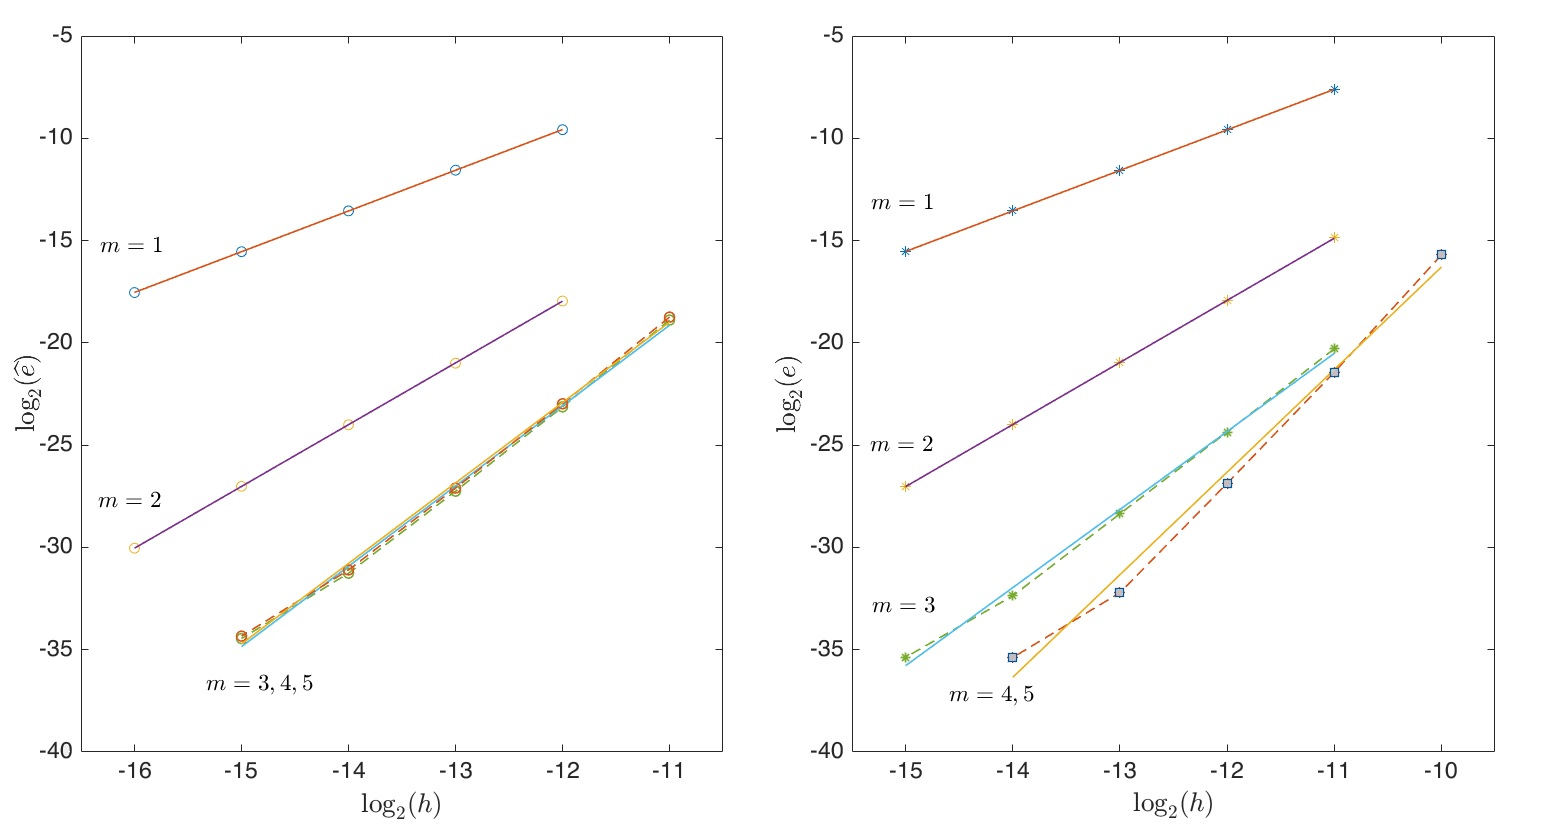
\includegraphics[scale=0.45]{Graphics/lldp/m-plots.jpg}
		\caption{Gráficos Log-log de los errores $\widehat{e}_i=\max_{t_n\in(t)_{h_i}}\nnnorm{\widehat{y}_n-x(t_n)}_\infty$ y $e_i=\max_{t_n\in(t)_{h_i}}\nnnorm{y_n-x(t_n)}_\infty$ contra $h_i$ en al integración del ejemplo \ref{ex:Brus} con las fórmulas (\ref{LLDPK scheme}), $\pf=6$, $\mf=1,2,3,4,5$ y $h_i=2^{-i}$, $i=10,11,12,13,14,15,16$.}
		\label{fig:num-exp-lldp-fix-step:Fig3}
	\end{center}
\end{figure}

\begin{table}[h]
	\centering
	\caption{
        Orden de convergencia $r$ de las fórmulas (\ref{LLDPK scheme}) y su estimado  $\widetilde{r}$ para diferentes valores de $\mf$, los $90\%$ límites de confianza $\Delta$ de $\widetilde {r}$, el coeficiente de determinación $R^2$ de la línea ajustada en la Figura \ref{fig:num-exp-lldp-fix-step:Fig3}.}
		\begin{tabular}{ c  c c c c  c  c c c c}
			\hline
			& \multicolumn{4}{c}{$\widehat{y}$} & & \multicolumn{4}{c}{$y$} \\
			\cline{2-5} \cline{7-10}
			$\mf$ & $r$ & $\widetilde{r}$ & $\pm\varDelta$ & $R^2$ & & $r$ & $\widetilde{r}$ & $\pm\varDelta$ & $R^2$ \\
			\hline
			1 & 2 & 1.99 & 0.01 & 0.99 & & 2 & 1.98 & 0.01 & 0.99 \\
			2 & 3 & 3.02 & 0.01 & 0.99 & & 3 & 3.04 & 0.01 & 0.99 \\
			3 & 4 & 3.93 & 0.20 & 0.99 & & 4 & 3.82 & 0.20 & 0.99 \\
			4 & 4 & 3.93 & 0.19 & 0.99 & & 5 & 5.02 & 0.45 & 0.99 \\
			5 & 4 & 3.93 & 0.19 & 0.99 & & 5 & 5.01 & 0.47 & 0.99 \\
			\hline
		\end{tabular}
	\label{tab:num-exp-lldp-fix-step:morders}
\end{table}

\begin{figure}[h]
	\begin{center}
		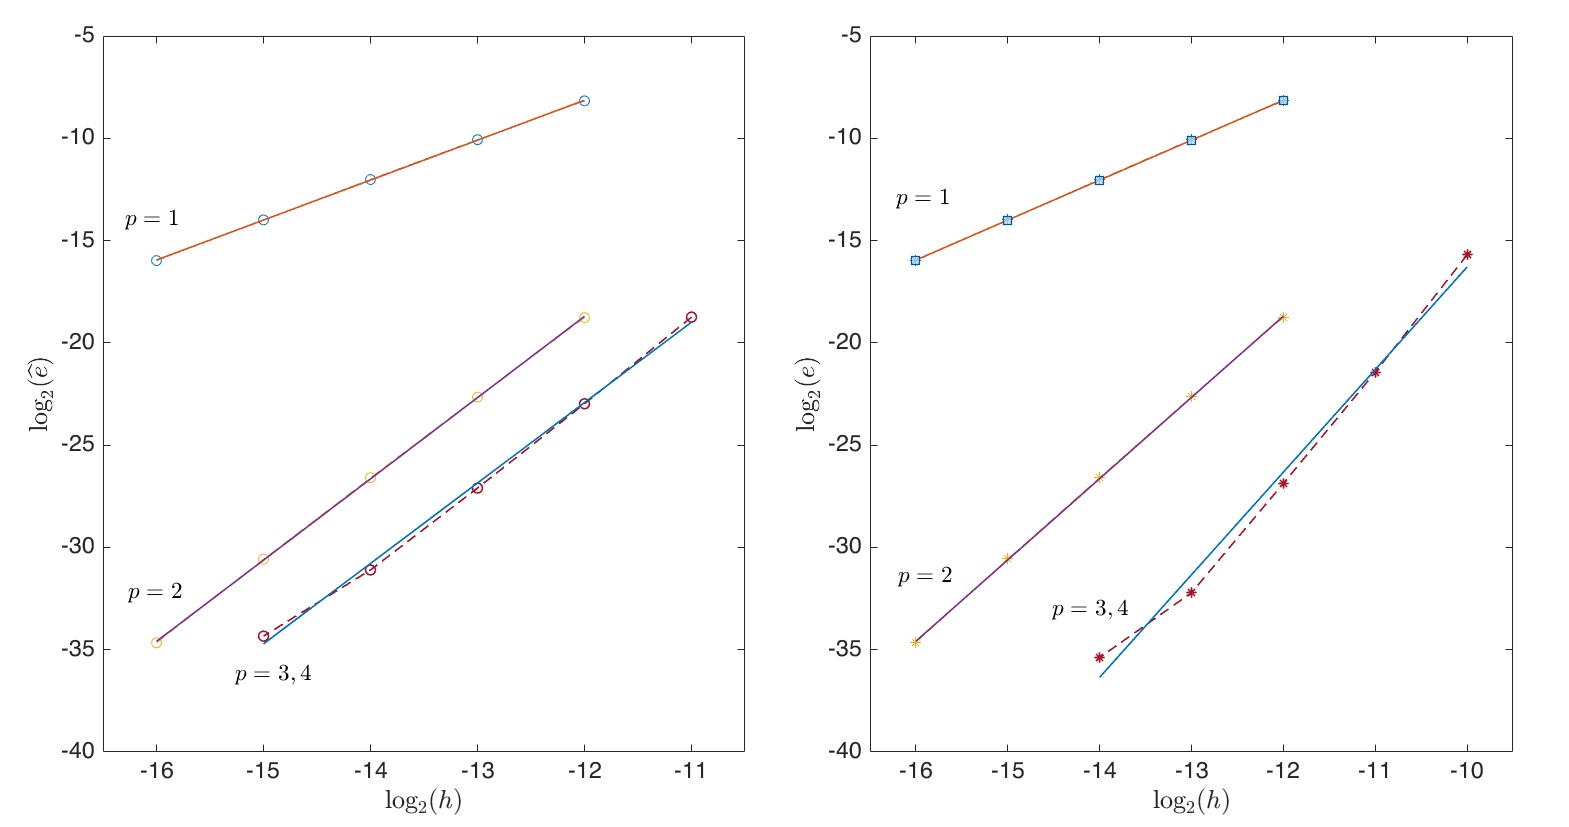
\includegraphics[scale=0.45]{Graphics/lldp/p-plots.jpg}
		\caption{Gráficos Log-log de los errores $\widehat{e}_i=\max_{t_n\in(t)_{h_i}}\nnnorm{\widehat{y}_n-x(t_n)}_\infty$ y $e_i=\max_{t_n\in(t)_{h_i}}\nnnorm{y_n-x(t_n)}_\infty$ contra $h_i$ en al integración del ejemplo \ref{ex:Brus} con las fórmulas (\ref{LLDPK scheme}), $\pf=1,2,3,4$, $\mf=11$ y $h_i=2^{-i}$, $i=10,11,12,13,14,15,16$.}
		\label{fig:num-exp-lldp-fix-step:Fig2}
	\end{center}
\end{figure}


\begin{table}[h]
	\centering
	\caption{
		Orden de convergencia $r$ de las fórmulas (\ref{LLDPK scheme}) y su estimado  $\widetilde{r}$ para diferentes valores de $\pf$, los $90\%$ límites de confianza $\Delta$ de $\widetilde {r}$, el coeficiente de determinación $R^2$ de la línea ajustada en la Figura \ref{fig:num-exp-lldp-fix-step:Fig2}.}
		\begin{tabular}{ c  c c c c  c  c c c c}
			\hline
			& \multicolumn{4}{c}{$\widehat{y}$} & & \multicolumn{4}{c}{$y$} \\
			\cline{2-5} \cline{7-10}
			$\pf+\pf$ & $r$ & $\widetilde{r}$ & $\pm\varDelta$ & $R^2$ & & $r$ & $\widetilde{r}$ & $\pm\varDelta$ & $R^2$ \\
			\hline
			2 & 2 & 1.95 & 0.02 & 0.99 & & 2 & 1.95 & 0.02 & 0.99 \\
			4 & 4 & 3.97 & 0.04 & 0.99 & & 4 & 3.97 & 0.04 & 0.99 \\
			6 & 4 & 3.93 & 0.19 & 0.99 & & 5 & 5.01 & 0.48 & 0.99 \\
			8 & 4 & 3.93 & 0.19 & 0.99 & & 5 & 5.01 & 0.47 & 0.99 \\
			\hline
		\end{tabular}
	\label{tab:num-exp-lldp-fix-step:porders}
\end{table}

\begin{figure}[h]
	\begin{center}
		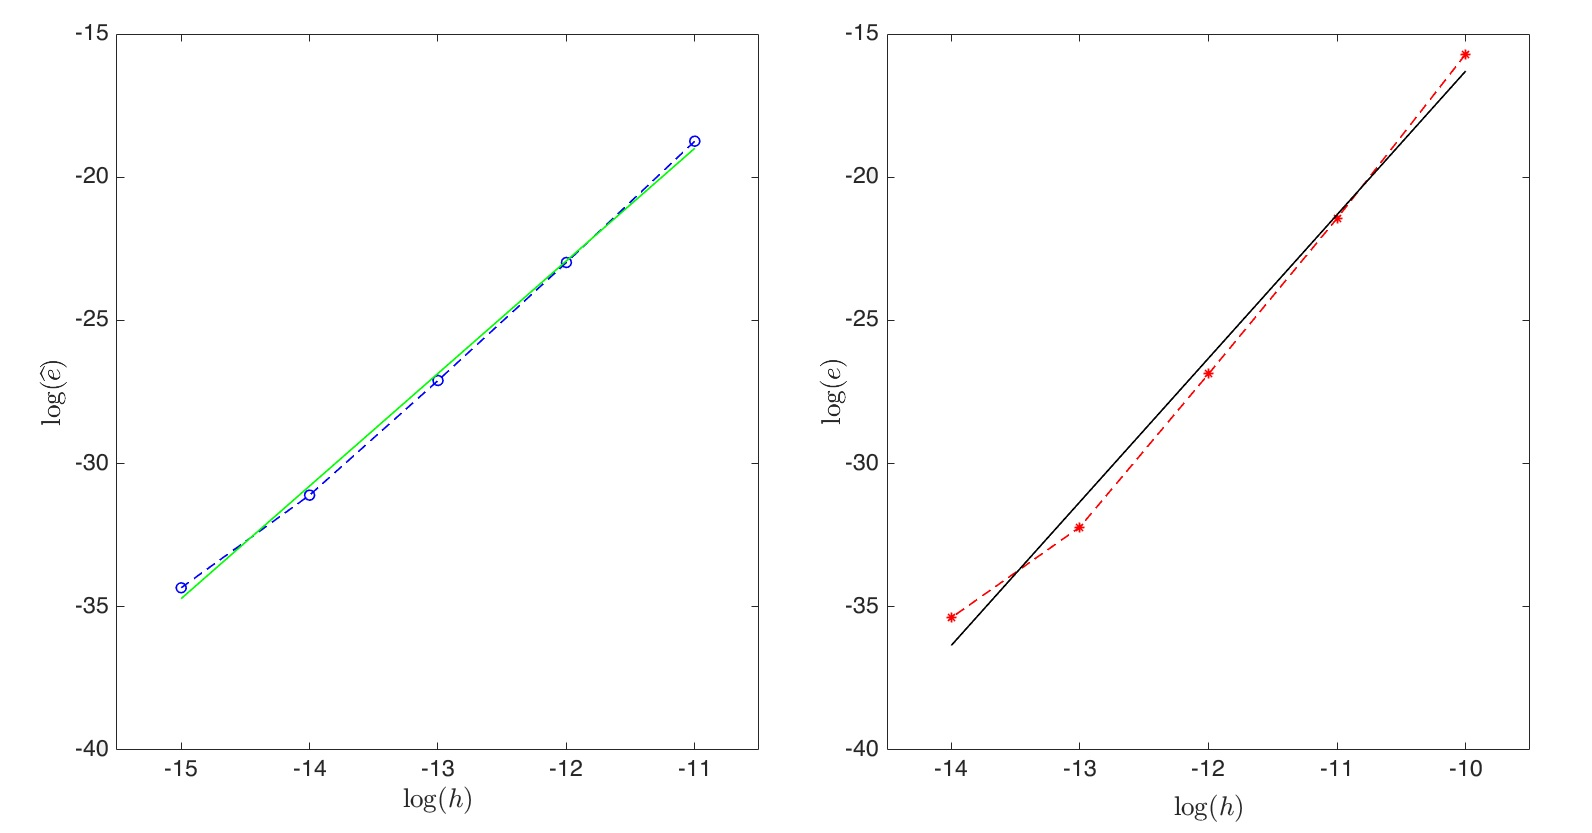
\includegraphics[scale=0.45]{Graphics/lldp/LLDP-plots.jpg}
		\caption{ Gráficos Log-log de los errores $\widehat{e}_i=\max_{t_n\in(t)_{h_i}}\nnnorm{\widehat{y}_n-x(t_n)}_\infty$ y $e_i=\max_{t_n\in(t)_{h_i}}\nnnorm{y_n-x(t_n)}_\infty$ contra $h_i$ en al integración del ejemplo \ref{ex:Brus} con las fórmulas (\ref{LLDPK scheme}), $\pf=6$, $\mf=11$ y $h_i=2^{-i}$, $i=10,11,12,13,14,15$.}
		\label{fig:num-exp-lldp-fix-step:Fig4}
	\end{center}
\end{figure}

\subsubsection{Simulaciones comparativas}
Para este segundo conjunto de simulaciones, se consideraran los esquemas numéricos definidos en el Algoritmo \ref{alg:integratorfix} para las fórmulas (\ref{LLDPK scheme}) de orden $4$ y $5$, que llamaremos \emph{LLDP} y \emph{LLDP5}, respectivamente. Además, se considerará, el código \textquoteleft expms\textquoteright~con orden $4$ y $5$ disponible en \cite{jansing2011expode}, que proporciona una implementación de tamaño de paso fijo de orden $4$ y $5$ para el método exponencial de Adams~\cite{hochbruck2011exponential}; se denotaran estos códigos exponenciales como \emph{expms4} y \emph{expms5}, respectivamente.

Para preservar el orden de convergencia de las fórmulas (\ref{LLDPK scheme}), se utilizaran los valores $m_{min}=3$ y $m_{min}=4$ en los códigos \emph{LLDP4} y \emph{LLDP5}, respectivamente, como lo indica el Teorema \ref{theorem:lldp-convergence}. Por el contrario, los códigos \emph{expms4} y \emph{expms5} no restringen los valores de $m_{min}$. Las tolerancias $RTol$ relativa y $ATol$ absoluta para calcular las aproximaciones de Krylov a $u_j$ se establecieron en $10^{-9}$ y $10^{-12}$, respectivamente.

Los resultados en la integración de cada ecuación de prueba obtenidos con los códigos antes mencionados se resumen en una tabla. La precisión de cada código se mide por el error relativo
\begin{equation}\label{num-exp-lldp-fix-step:ER}
	RError = \max_{i=1,\ldots,d} \;\ \max_{t_n\in(t)_h}  \;\ \left\lvert\frac{x^{[i]}(t_j)-y^{[i]}(t_j)}{\maxx{x^{[i]}(t_j),\epsilon_{mach}}}\right\rvert
\end{equation}
entre la \textquotedblleft solución exacta\textquotedblright~$x$ de la ecuación de prueba y la solución aproximada $y$ de cada código, donde $\epsilon_{mach}$ denota el espaciado en coma flotante del número $1$. Siguiendo \cite{tokman2006efficient}, la \textquotedblleft solución exacta\textquotedblright de las ecuaciones de prueba se estima mediante el código Matlab \textit{ode15s} con tolerancias $RTol=10^{-12}$ y $ATol=10^{-14}$. En cada tabla, la columna \textit{RTime} presenta el tiempo computacional total relativo de cada código con respecto al código \emph{expms4} en la integración de cada ejemplo. Esta relación de tiempo general funciona como un indicador simple para comparar el costo computacional total de cada código. Las tablas también muestran el número de pasos de integración $Steps$, el número de evaluaciones de campos vectoriales \textit{f-Eval}, el número de evaluaciones de la matriz Jacobianas \textit{J-Eval}, el número de aproximaciones del subespacio de Krylov \textit{K-subspace}, la dimensión mínima $\mf_{min}$, la dimensión máxima $\mf_{max}$ y la dimensión total $\mf_{total}$ de los subespacios de Krylov utilizados por cada código en la integración de la prueba ecuaciones con tamaño de paso $h$, donde $m_{total}$ es la suma acumulada de la dimensión de los subespacios de Krylov utilizada en cada paso de integración.

Las Tablas \ref{tab:num-exp-lldp-fix-step:cpna} - \ref{tab:num-exp-lldp-fix-step:brna} presentan los resultados de la integración de las ecuaciones de prueba de los ejemplos \ref{ex:cusp}-\ref{ex:Brus}, que muestran que, con tamaño de paso fijo y dimensión variable de Krylov, los códigos \emph{LLDP4} y \emph{LLDP5} son más precisos que los códigos \emph{expms4} y \emph{expms5}, con un costo computacional similar o menor. Los códigos \emph{LLDP} son más rápidos porque requieren el cálculo de solo un subespacio de Krylov por paso de integración con dimensiones más pequeñas, mientras que los otros códigos calculan más de un subespacio de Krylov con dimensiones más altas. El código \emph{LLDP5} es más rápido que el \emph{LLDP4} porque la fórmula de orden 4 en (\ref{LLDPK scheme}) requiere de una evaluación adicional del campo vectorial $f$ en cada paso de integración. Con tamaño de paso $h = 0.0064$, el código \emph{expms5} produce desbordamiento en la integración de la ecuación de Burges, razón por la cual falta información en la Tabla \ref{tab:num-exp-lldp-fix-step:bgna}. Por la misma razón, falta un valor en la Tabla \ref{tab:num-exp-lldp-fix-step:brna} para el código \emph{expms5} con un tamaño de paso $h = 0.0008$.

Además, las tablas muestran la efectividad de la estrategia propuesta para la selección de la dimensión de Krylov $\mf$ en cada paso de integración, con mínima variación entre los valores de $\mf_{min}$ y $\mf_{max}$, y así, con un valor menor de $\mf_{total}$.

\begin{table}[h]
	\caption{Desempeño de los códigos \emph{expms4}, \emph{expms5}, \emph{LLDP4} y \emph{LLDP5} en la integración de la ecuación CUSP con $M=32$, $d=96$.}
	\centering
		\begin{tabular}{lccccccccc}
			\hline
			& RTime & RError & Steps & f-Eval & J-Eval & K-subspace & $\mf_{total}$ & $\mf_{min}$ & $\mf_{max}$ \\
			\hline
			h = 0.000001 &  &  &  &  &  &  &  &  &  \\
			expms4 & 1.0000 & 8.4400e-01 & 100 & 204 & 100 & 298 & 1131 & 2 & 6  \\
			expms5 & 1.1863 & 6.1635e-01 & 100 & 209 & 100 & 397 & 1336 & 2 & 6  \\
			LLDP4 & 0.1013 & 3.8321e-08 & 100 & 700 & 100 & 100 & 400 & 4 & 4  \\
			LLDP5 & 0.0863 & 1.0889e-09 & 100 & 600 & 100 & 100 & 400 & 4 & 4  \\
			\hline
			h = 0.000005 &  &  &  &  &  &  &  &  &  \\
			expms4 & 1.0000 & 9.7513e-01 & 20 & 44 & 20 & 58 & 381 & 4 & 11  \\
			expms5 & 1.0480 & 1.0766e+00 & 20 & 49 & 20 & 77 & 593 & 4 & 20  \\
			LLDP4 & 0.0354 & 4.5302e-06 & 20 & 140 & 20 & 20 & 130 & 6 & 7  \\
			LLDP5 & 0.0338 & 2.0199e-07 & 20 & 120 & 20 & 20 & 130 & 6 & 7  \\
			\hline
			h = 0.000010 &  &  &  &  &  &  &  &  &  \\
			expms4 & 1.0000 & 1.7607e+00 & 10 & 24 & 10 & 28 & 378 & 6 & 36  \\
			expms5 & 1.1111 & 3.5472e+02 & 10 & 29 & 10 & 37 & 586 & 6 & 36  \\
			LLDP4 & 0.0228 & 4.4774e-05 & 10 & 70 & 10 & 10 & 83 & 7 & 10  \\
			LLDP5 & 0.0214 & 1.3267e-05 & 10 & 60 & 10 & 10 & 83 & 7 & 10  \\
			\hline
		\end{tabular}
	\label{tab:num-exp-lldp-fix-step:cpna}
\end{table}



\begin{table}[h]
	\caption{Desempeño de los códigos \emph{expms4}, \emph{expms5}, \emph{LLDP4} y \emph{LLDP5} en la integración de la ecuación Burgers con $M=500$, $d=500$.}
	\centering
	\begin{tabular}{lccccccccc}
		\hline
		& RTime & RError & Steps & f-Eval & J-Eval & K-subspace & $\mf_{total}$ & $\mf_{min}$ & $\mf_{max}$ \\
		\hline
		h = 0.001600 &  &  &  &  &  &  &  &  &  \\
		expms4 & 1.0000 & 2.0411e-03 & 313 & 630 & 313 & 937 & 5984 & 2 & 11  \\
		expms5 & 1.3115 & 6.2805e-04 & 313 & 635 & 313 & 1249 & 7744 & 2 & 11  \\
		LLDP4 & 0.1109 & 3.7647e-06 & 313 & 2191 & 313 & 313 & 2174 & 4 & 8  \\
		LLDP5 & 0.1081 & 6.8065e-07 & 313 & 1878 & 313 & 313 & 2174 & 4 & 8  \\
		\hline
		h = 0.003200 &  &  &  &  &  &  &  &  &  \\
		expms4 & 1.0000 & 2.0005e-02 & 157 & 318 & 157 & 469 & 5802 & 3 & 46  \\
		expms5 & 1.2350 & 1.1603e-02 & 157 & 323 & 157 & 625 & 7747 & 3 & 57  \\
		LLDP4 & 0.0719 & 7.8449e-05 & 157 & 1099 & 157 & 157 & 1425 & 6 & 10  \\
		LLDP5 & 0.0719 & 4.5654e-05 & 157 & 942 & 157 & 157 & 1425 & 6 & 10  \\
		\hline
		h = 0.006400 &  &  &  &  &  &  &  &  &  \\
		expms4 & 1.0000 & 5.7742e-01 & 79 & 162 & 79 & 235 & 6267 & 6 & 100  \\
		expms5 & - & - & - & - & - & - &- & - & -\\
		LLDP4 & 0.0281 & 2.3688e-03 & 79 & 553 & 79 & 79 & 954 & 8 & 14  \\
		LLDP5 & 0.0278 & 3.6646e-03 & 79 & 474 & 79 & 79 & 964 & 8 & 15  \\
		\hline
	\end{tabular}
	\label{tab:num-exp-lldp-fix-step:bgna}
\end{table}


\begin{table}[h]
	\caption{Desempeño de los códigos \emph{expms4}, \emph{expms5}, \emph{LLDP4} y \emph{LLDP5} en la integración de la ecuación Brusselator2D con $M=50$, $d=5000$.}
	\centering
	\begin{tabular}{lccccccccc}
		\hline
		& RTime & RError & Steps & f-Eval & J-Eval & K-subspace & $\mf_{total}$ & $\mf_{min}$ & $\mf_{max}$ \\
		\hline
		h = 0.000313 &  &  &  &  &  &  &  &  &  \\
		expms4 & 1.0000 & 2.7423e-09 & 320 & 644 & 320 & 958 & 1702 & 1 & 6  \\
		expms5 & 1.3830 & 2.6788e-09 & 320 & 649 & 320 & 1277 & 2023 & 1 & 6  \\
		LLDP4 & 0.7161 & 1.9118e-10 & 320 & 2240 & 320 & 320 & 960 & 3 & 3  \\
		LLDP5 & 0.7158 & 9.6701e-12 & 320 & 1920 & 320 & 320 & 1280 & 4 & 4  \\
		\hline
		h = 0.006250 &  &  &  &  &  &  &  &  &  \\
		expms4 & 1.0000 & 7.7678e-06 & 16 & 36 & 16 & 46 & 231 & 3 & 11  \\
		expms5 & 1.1151 & 3.5951e-06 & 16 & 41 & 16 & 61 & 283 & 2 & 11  \\
		LLDP4 & 0.2909 & 1.7453e-08 & 16 & 112 & 16 & 16 & 115 & 6 & 9  \\
		LLDP5 & 0.2592 & 4.8969e-09 & 16 & 96 & 16 & 16 & 115 & 6 & 9  \\
		\hline
		h = 0.012500 &  &  &  &  &  &  &  &  &  \\
		expms4 & 1.0000 & 5.4570e-05 & 8 & 20 & 8 & 22 & 163 & 4 & 15  \\
		expms5 & 1.0989 & 3.1705e-05 & 8 & 25 & 8 & 29 & 213 & 4 & 15  \\
		LLDP4 & 0.1990 & 1.6384e-07 & 8 & 56 & 8 & 8 & 74 & 8 & 11  \\
		LLDP5 & 0.1783 & 9.7264e-08 & 8 & 48 & 8 & 8 & 74 & 8 & 11  \\
		\hline
	\end{tabular}
	\label{tab:num-exp-lldp-fix-step:br2dna}
\end{table}

\begin{table}[h]
	\caption{Desempeño de los códigos \emph{expms4}, \emph{expms5}, \emph{LLDP4} y \emph{LLDP5} en la integración de la ecuación Brusselator con $M=100$, $d=200$.}
	\centering
	\begin{tabular}{lccccccccc}
		\hline
		& RTime & RError & Steps & f-Eval & J-Eval & K-subspace & $\mf_{total}$ & $\mf_{min}$ & $\mf_{max}$ \\
		\hline
		h = 0.000200 &  &  &  &  &  &  &  &  &  \\
		expms4 & 1.0000 & 1.8209e-01 & 5000 & 10004 & 5000 & 14998 & 37224 & 1 & 6  \\
		expms5 & 1.2761 & 2.2454e-01 & 5000 & 10009 & 5000 & 19997 & 42325 & 1 & 6  \\
		LLDP4 & 0.1876 & 4.2112e-08 & 5000 & 35000 & 5000 & 5000 & 15491 & 3 & 6  \\
		LLDP5 & 0.1839 & 2.3705e-09 & 5000 & 30000 & 5000 & 5000 & 20004 & 4 & 6  \\
		\hline
		h = 0.000400 &  &  &  &  &  &  &  &  &  \\
		expms4 & 1.0000 & 3.6729e-01 & 2500 & 5004 & 2500 & 7498 & 23266 & 1 & 8  \\
		expms5 & 1.2349 & 4.4819e-01 & 2500 & 5009 & 2500 & 9997 & 25921 & 1 & 8  \\
		LLDP4 & 0.1915 & 7.8097e-07 & 2500 & 17500 & 2500 & 2500 & 10068 & 4 & 6  \\
		LLDP5 & 0.1621 & 9.7577e-08 & 2500 & 15000 & 2500 & 2500 & 10068 & 4 & 6  \\
		\hline
		h = 0.000800 &  &  &  &  &  &  &  &  &  \\
		expms4 & 1.0000 & 7.2534e-01 & 1250 & 2504 & 1250 & 3748 & 15258 & 2 & 8  \\
		expms5 & - & - & - & - & - & - &- & - & -\\
		LLDP4 & 0.1873 & 1.5639e-05 & 1250 & 8750 & 1250 & 1250 & 7517 & 6 & 8  \\
		LLDP5 & 0.1805 & 4.6983e-06 & 1250 & 7500 & 1250 & 1250 & 7517 & 6 & 8  \\
		\hline
	\end{tabular}
	\label{tab:num-exp-lldp-fix-step:brna}
\end{table}

\section{Esquemas adaptativos con tamaño de paso variable}
Para escribir un código que determine automáticamente el tamaños de paso lo suficientemente pequeños para obtener la precisión adecuada y lo suficientemente grandes para evitar trabajo computacional innecesario, es necesaria una estrategia adaptativa adecuada. Como se mostró en \cite{Jimenez14AMC}, el control del tamaño de paso automático de las fórmulas embebidas originales de Runge-Kutta de Dormand y Prince se adapta bien a las fórmulas embebidas (\ref{LLDPK scheme}) para PVI pequeños. Es fácil notar que con ciertas modificaciones relacionadas con la aproximación Krylov-Padé (\ref{eq:kp_aprox}), esta estrategia para la selección del tamaño del paso parece adecuada para las fórmulas embebidas (\ref{LLDPK scheme}) para PVI grandes. A continuación, se describirá la estrategia adaptativa para las fórmulas embebidas (\ref{LLDPK scheme}).

\subsection{Estimación del tamaño de paso}\label{secc:stepsizes}
Se denotará $h_{max}$ y $h_{min}$ como los tamaños de paso máximos y mínimos permisibles. La estimación de los tamaños de paso se calcula mediante las mismas expresiones utilizadas para las fórmulas originales de Dormand y Prince en el código de Matlab \textit{ode45} \cite{shampine1997matlab} y para las fórmulas embebidas en \cite{Jimenez14AMC}. Para el tamaño de paso inicial $h_0$, tenemos la estimación
\begin{equation}
    h_0 = \minn{ h_{max}, \maxx{ h_{min} ,\Delta} }, \label{hcero}
\end{equation}
donde
\begin{equation*}
    \Delta = \begin{cases}
        \frac{1}{r_h} & \text{if} \; h_{max}\cdot r_h>1\\
        h_{max} & \text{en otro casos}
        \end{cases}
\end{equation*}
con
\begin{equation*}
     r_h = \frac{1\mathord{.}25}{RTol^{1/5}}\max_{i=1\ldots d}\left\{\frac{ \left\lvert f^{[i]}(t_0,y_0) \right\rvert }
    {\maxx{\left\lvert y^{[i]}_0 \right\rvert ,\frac{ATol}{RTol}}}\right\}.
\end{equation*}

Todos los demás tamaños de paso nuevos $h_{new}$ se estiman mediante la expresión
\begin{equation}
    h_{new} = \minn{h_{max},\maxx{h_{min},\Delta}}, \label{hnewcalc}
\end{equation}
donde
\begin{equation*}
    \Delta = \begin{cases}
        h_n/\rho & \text{if } \varepsilon_y\leq RTol \text{ y } \rho>0\mathord{.}2\\
        5\cdot h_n & \text{if } \varepsilon_y\leq RTol \text{ y } \rho\leq 0\mathord{.}2\\
        \maxx{0\mathord{.}1,1/\rho}\cdot h_n & \text{if } \varepsilon_y > RTol \text{ y } fail=false\\
        0\mathord{.}5\cdot h_n & \text{if } \varepsilon_y > RTol \text{ y } fail=true
        \end{cases},
\end{equation*}
siendo
\begin{equation}\label{epsilon_y}
	\varepsilon_y =  \max_{i=1\ldots d}\left\{ \frac{\left\lvert y^{[i]}_{n+1}-\hat{y}^{[i]}_{n+1} \right\rvert}
	{\maxx{\left\lvert y^{[i]}_{n+1}  \right\rvert,\left\lvert y^{[i]}_{n}\right\rvert,\frac{ATol}{RTol}}} \right\}
\end{equation}
la medida del error relativo entre las fórmulas integradas $y$ y $\hat{y}$ definidas en (\ref{LLDPK scheme}), y $fail$ indica que se rechazó un tamaño de paso anterior en $t_n$.

\subsection{Control del tamaño de paso}\label{secc:hcontrol}
Como en \cite{Jimenez14AMC}, para obtener una tolerancia deseada y evitar el desbordamiento en el cálculo de la matriz exponencial $e^{\frac{1}{90}h_n\overline{H}}$ a través de la aproximación $(\pf,\pf)$-Padé con escalamiento y potenciación, el valor de $\left\Vert \frac{1}{90}h_n\overline{H} \right\Vert_\infty$ debe ser controlado. Debido a los errores de redondeo, si $\left\Vert \frac{1}{90}h_n\overline{H} \right\Vert_\infty \ge 600$, la aproximación de Padé a $e^{\frac{1 }{90}h_n\overline{H}}$ carece de precisión. Dado que $H_\mf$ in (\ref{hhat}) es la matriz superior de Hessenberg correspondiente a $\mathcal{K}_\mf(f_x,f)$, el Lema \ref{H-bound} implica que $|| \overline{H} ||_\infty \leq 1 + || f_x ||_\infty$. Por lo tanto, si $h_n + \left\lVert h_nf_x \right\rVert_\infty \leq 54000$, entonces la aproximación $(\pf,\pf)$-Padé de $e^{\frac{1}{90}h_n \overline{H}}$ conserva la precisión establecida en la Tabla \ref{table:padep} para el valor dado de $\pf$. Así, en la práctica, si $h_n + \left\lVert h_nf_x \right\rVert_\infty \ge 54000$, el valor de $h_n$ se restablece como $h_n=\frac{54000}{1+\left\lVert f_x \right\rVert_\infty}$.

Aqui hay que tener en cuenta que en el caso de que se modifique el valor del tamaño de paso $h_{n}$, la evaluación de $f$ y $f_x$ en $y_n$ realizada para calcular $\overline{H}$ es reutilizada. Por lo tanto, este reemplazo de tamaño de paso no se considera como un paso fallido ``típico" .

\subsection{Reutilización de la matriz Jacobiana}\label{secc:jaccontrol}
Ciertamente, para grandes PVI almacenar y evaluar la matriz Jacobiana $f_x$ de $f$ en cada paso de integración es una tarea computacionalmente exigente. Por lo general, la matriz Jacobiana de grandes sistemas resultantes de la discretización espacial de las EDP tiene una estructura esparcida. En esta situación, en la práctica es posible almacenar y reutilizar esas matrices. Para determinar cuándo el Jacobiano evaluado en un paso de integración se puede reutilizar en pasos de integración consecutivos, una medida de disimilitud entre el Jacobiano $J=f_x(y_n)$ en el paso de integración actual $n$ con el Jacobiano $J_{old}= f_x(y_{i})$ en un paso de integración anterior $i<n$ es necesario. Una de tales medidas de disimilitud se puede definir en términos de
\begin{equation*}
    \Delta \mathcal{J} = J\cdot f(y_n) - J_{old}\cdot f(y_n),
\end{equation*}
o por la expresión relativa
\begin{equation}\label{jerror}
    \varepsilon_J = \max_{i=1\ldots d}\frac{\nnorm{\Delta \mathcal{J}^{[i]}}}
    {\maxx{\nnorm{ \left(J_{old}\cdot f_{old}\right)^{[i]} } ,\frac{ATol}{RTol}}},
\end{equation}
donde $f_{old}=f(y_i)$.

Dado que en la expresión ~(\ref{jerror}) se supone que el Jacobiano $J$ en $y_n$ no se evalúa, el término $J\cdot f(y_n)$ es
aproximado por el cociente diferencial hacia atrás
\begin{equation}\label{backapprox}
    J\cdot f(y_n) \approx \frac{f(y_n) -
        f\left(y_n-\delta f(y_n)\right)}{\delta}
\end{equation}
para un $\delta>0$ lo suficientemente pequeño. Pero, en esta aproximación se requiere la evaluación de $f$ en un punto medio. Para evitar esto, se puede usar la aproximación convexa
\begin{equation}\label{aproxaprox}
    f\left(y_n-\delta f(y_n)\right) \approx
    (1-\delta) f(y_n)+ \delta \; \mathtt{K},
\end{equation}
donde $K = \kt_{6} + f(y_{n-1}) + J_{old}\widetilde{u}_{6} $ y
\[ \kt_6 = f\left( y_{n-1}+\widetilde{u}_6+h_{n-1} \sum_{i=1}^{5}a_{6,i}\kt_i \right) - f(y_{n-1}) - J_{old}\widetilde{u}_6 \]
es el estado $6$ del esquema~(\ref{LLDPK scheme}) ya calculado en el paso anterior $n-1$.

Es importante notar que el campo vectorial $f$ en el punto actual $y_n$ tiene el mayor peso en la aproximación porque $\delta$
es pequeño. Sustituyendo~(\ref{backapprox})-(\ref{aproxaprox}) en (\ref{jerror}) se obtiene que
\begin{equation}\label{jerroraprox}
    \varepsilon_J = \max_{i=1\ldots d}\frac{\nnorm{f^{[i]}(y_n) - \mathtt{K}^{[i]} - (J_{old}\cdot f(y_n))^{[i]}}}
    {\maxx{\nnorm{ \left(J_{old}\cdot f_{old}\right)^{[i]} } ,\frac{ATol}{RTol}}}.
\end{equation}

Con esta medida relativa de disimilitud, el Jacobiano se evalúa en el punto $y_n$ solo si $\gamma_J \cdot \varepsilon_J \geq 1$, donde $\gamma_J=\frac{1}{8}$ es un factor de seguridad. Este procedimiento para la reutilización de la matriz Jacobiana se resume en las líneas 3 a 12 del Algoritmo \ref{alg:jaccontrol} y se utiliza siempre que el tamaño de paso $h_n$ en el paso de integración $n$ no haya sido rechazado previamente. De lo contrario, el Jacobiano siempre se actualiza como se indica en las líneas 15 a 20 del mismo Algoritmo.

{\SetAlgoNoLine
\begin{algorithm}[h]
	\caption{Control de Reutilización del Jacobiano}
	\label{alg:jaccontrol}
	\KwIn{$n$,$y_n$,$fail,J,J_{old},f_{old},freshJ$}
	\KwOut{$J,J_{old},f_{old},freshJ$}
	\eIf{$fail=false$}{
		\If{$n>0$}{
			Calcular la medida relativa de disimilitud $\varepsilon_J$ mediante (\ref{jerroraprox})\\
			\eIf{$\gamma_J\cdot\varepsilon_J \geq 1$}{
				$J=f_x(y_n)$ \\
				$J_{old} = J$ \\
				$f_{old} = f(y_n)$ \\
				$freshJ=true$ \\
			}
			{
				$J=J_{old}$ \\
				$freshJ=false$ \\
			}
		}
	}
	{
		\If{$freshJ=false$}{
			$J=f_x(y_n)$ \\
			$J_{old} = J$ \\
			$f_{old} = f(y_n)$ \\
			$freshJ=true$ \\
		}
	}
\end{algorithm}
}

\subsection{Control del \textit{Breakdown}}\label{sec:brcontrol}
El \emph{breakdown} en el Algoritmo de Arnoldi~\ref{alg:Arnoldi}, línea $10$, puede ocurrir por la pérdida de ortogonalidad al generar los vectores base como consecuencia de la acumulación de errores de redondeo. Por esta razón, el Algoritmo~\ref{alg:Arnoldi} tiene una parada anticipada y el último vector en la base es inútil. Cuando ocurre \emph{breakdown} tenemos dos situaciones: 1) $\varepsilon_{K}/\gamma_K< 1$, o 2) $\varepsilon_{K}/\gamma_K \geq 1$ donde $\varepsilon_{K}$ es el error relativo (\ref{errrel}) y $\gamma_K$ su factor de seguridad.

En el caso de que $\varepsilon_{K}/\gamma_K< 1$, se acepta la aproximación de Krylov. De lo contrario, la aproximación de Krylov-Padé no satisface los requisitos de tolerancia y se calcula un nuevo valor de $h_n$. Con $h_{old}=h_n$, el nuevo valor del tamaño del paso se calcula como $h_n=\maxx{h_{min},0.9\cdot h_{old}}$. De esta forma, se debe calcular también un nuevo valor del orden de Padé $\pf$ y de la medida de disimilitud $\varepsilon_{K}$.

\subsection{Aproximación Krylov-Padé adaptativa}\label{secc:krylov-Pade}
Mediante una combinación adecuada de los procedimientos de las Secciones \ref{sec:selkrydim} y \ref{sec:brcontrol} para la estimación de una dimensión Krylov adecuada $\mf$, y el criterio de la Sección \ref{sec:pade-order} para la estimación de un orden de Padé adecuado $\pf$, el Algoritmo \ref{alg:errcontrol} presenta el esquema adaptativo de la aproximación de Krylov-Padé para $u_j$ en cada paso de integración.

{\SetAlgoNoLine
\begin{algorithm}[h!]
	\caption{Cálculo de $u_j$ mediante la aproximación adaptativa Krylov-Padé}
	\label{alg:errcontrol}
	\KwIn{$c_j$, $h_n$, $J$, $f$, $\mf_n$, $V_{\mf_n}$, $H_{\mf_n}$,
		$v_{\mf_{n}+1}$,  $\hf_{\mf_{n}+1,\mf_n}$, $H^*_{m_{n}}$, $breakdown$}
	\KwOut{$\widetilde{u }_j$, $h_n$, $\mf_n$, $V_{\mf_n}$,   $H_{\mf_n}$,
		$v_{\mf_{n}+1}$,  $\hf_{\mf_{n}+1,\mf_n}$, $H^*_{m_{n}}$, $\varepsilon_{K}$}
	$work=true$\\
	\While{work}{
		Selecionar el orden de Padé $\pf$ según Sección \ref{sec:pade-order} \\
		Estimar el error relativo $\varepsilon_{K}$ mediante fórmula~(\ref{errrel}) \\
		\eIf{$\varepsilon_{K}/\gamma_{K}< 1$}{
			$work=false$
		}{
			\eIf{$breakdown$ = $true$ \textbf{or} $\mf_n=\mf_{max}$}{
				$h_{new}=\maxx{h_{min},0.9\cdot h_{n}}$\\
				$h_{n}=h_{new}$\\
				\If{$h_n = h_{min}$}{work = false}
			}{
				Estimar la nueva dimensión de Krylov $\mf_{new}$ mediante fórmula
				(\ref{calcmnew}) \\
				Ejecutar Algoritmo~\ref{alg:Arnoldiexpand} para obtener matrices $H^*_{m_{new}}$ y $V_{m_{new}}$ de $\mathcal{K}_{\mf_{new}}(h_nJ,f)$ y establecer el valor $H_{m_{new}}=H^*_{m_{new}}/h_n$\\
				establecer el valor $\mf_n=\mf_{new}$ y actualizar todas las variables que dependen de $\mf_n$,
			}
		}

	}
	Calcular $\widetilde{u}_j$ mediante la fórmula (\ref{eq:kp_aprox})\\
\end{algorithm}}

\subsection{Esbozo del Esquema}

Teniendo en cuenta los procedimientos de las Secciones \ref{secc:stepsizes} y \ref{secc:hcontrol} para la estimación y control del tamaño de paso $h_n$, el criterio de la Sección \ref{secc:jaccontrol} para la reutilización del Jacobiano, y la aproximación adaptativa de Krylov-Padé a $u_j$ descrita en la Sección \ref{secc:krylov-Pade}, el Algoritmo \ref{alg:integrator} presenta el esquema de la estrategia adaptativa para las fórmulas embebidas  (\ref{LLDPK scheme}) con tamaño de paso variable y dimensión Krylov. Obsérvese que, para tamaños de paso no fallidos, el Algoritmo \ref{alg:Arnoldi} se llama solo una vez por paso de integración. Cuando se rechaza un tamaño de paso $h_n$, se llama al Algoritmo \ref{alg:Arnoldi} solo cuando la matriz Jacobiana no se ha actualizado en $y_n$, es decir, cuando $J \neq f_x(y_n)$.


{\SetAlgoNoLine
\begin{algorithm}[h]
	\caption{Esquema con tamaño de paso y dimensión de Krylov variables}
	\label{alg:integrator}
	\KwIn{intervalo de tiempo $[t_0, T]$, valor inicial $y_0$, tolerancia absoluta y relativa $Atol$ y $Rtol$, dimensión máxima y mínima de los subespacios de Krylov $\mf_{max}$ y $\mf_{min}$, tamaño de paso máximo $h_{max}$}
	\KwOut{$\{(t_0,y_0),\ldots,(t_n,y_n)\}$}
	$n=0$, $fail=false$, $reuse=false$, $\mf_0=\mf_{min}$, $h_{min}=16 \cdot \epsilon(t_0)$ \\
	Calcular $h_0$ mediante fórmula (\ref{hcero}) \\
	$J = f_x(y_n)$ \\
	$J_{old} = J$, $freshJ=true$ \\
	$f_{old} = f(y_n)$ \\
	\While{$t_n<T$}{
		Control de reutilización del Jacobiano mediante Algoritmo~\ref{alg:jaccontrol} \\
		Control del tamaño de paso como se especifica en la sección~\ref{secc:hcontrol} \\
		\If{$fail=false$ or $reuse=false$}{
			Ejecutar Algoritmo~\ref{alg:Arnoldi} para obtener matrices $H^*_{m_n}$ y $V_{m_n}$ de $\mathcal{K}_{\mf_n}(h_nJ,f)$ y establecer el valor $H_{m_n}=H^*_{m_n}/h_n$ \\
		}
		Calcular $\widetilde{u}_j$ mediante Algoritmo~\ref{alg:errcontrol}\\
		Evaluar las fórmulas embebidas (\ref{LLDPK scheme}) \\
		Estimar el error de las formulas embebidas (\ref{epsilon_y}) \\
		Estimar la nueva dimensión de Krylov $\mf_{new}$ mediante fórmula (\ref{calcmnew}) \\
		Estimar le nuevo tamaño de paso $h_{new}$ mediante fórmula (\ref{hnewcalc}) \\
		\eIf{$\varepsilon_y< RTol$}{
			\If{$t_n+h_n+h_{new}>T$}{
				$h_{new}=T-(t_n+h_n)$ \\
			}
			$t_{n+1}=t_n+h_n$, $n=n+1$, $h_n=h_{new}$, $\mf_n = \mf_{new}$, $fail=false$, $reuse=false$ \\
		}
		{
			\eIf{$h_{new}>h_{min}$}
			{
				$h_n=h_{new}$, $\mf_n = \mf_{new}$, $fail = true$, $reuse=fail\,\&freshJ$
			}
			{$t_{n+1}=t_n+h_n$, $n=n+1$, $h_n=h_{new}$, $\mf_n = \mf_{new}$, $fail=false$, $reuse=false$}
		}
	$h_{min}=16 \cdot \epsilon(t_n)$
	}
\end{algorithm}}

\subsection{Experimentos numéricos}\label{section:num-exp-lldp-var-step}
Con este conjunto de simulaciones, se estudiará el desempeño del esquema adaptativo descrito en el Algoritmo \ref{alg:integrator} para las fórmulas embebidas (\ref{LLDPK scheme}). Con este propósito se construyó el código Matlab \emph{LLDP45}. Este código \emph{LLDP45} es una copia exacta del código Matlab18a \emph{ode45} \cite{shampine1997matlab} con la excepción de las líneas del programa correspondientes a las fórmulas originales de Dormand y Prince y su error relativo, que fueron reemplazadas por las líneas 7 a 16 del Algoritmo \ref{alg:integrator} que implementan la evaluación de las fórmulas localmente linealizadas (\ref{LLDPK scheme}) con control de reutilización del Jacobiano. El código de Matlab \emph{ode45} implementa la estrategia de tamaño de paso variable descrita en la Sección \ref{secc:stepsizes} para las fórmulas embebidas de Runge-Kutta de Dormand y Prince. Para preservar el orden de convergencia establecido en el Teorema \ref{theorem:lldp-convergence} para las fórmulas embebidas (\ref{LLDPK scheme}), se establece $m_{min}=4$ en el código \emph{LLDP45}.

Los resultados del código \emph{LLDP45} en la integración de las ecuaciones de prueba de Sección \ref{section:test-eq} se compararán con los obtenidos por el código adaptativo \emph{ode15sk} con una implementación de tamaño de paso casi constante de las fórmulas diferenciales hacia atrás (BDF) hasta orden 5 y un método de subespacios de Krylov para resolver sistemas lineales de ecuaciones algebraicas. Para comparar con una implementación eficiente de estas fórmulas, este código \emph{ode15sk} es una copia exacta del código Matlab18a \emph{ode15s} \cite{shampine1997matlab} con la excepción de las líneas de programa correspondientes a los métodos directos (función Matlab \emph{mldivide}) para resolver sistemas lineales de ecuaciones algebraicas y la factorización LU, que fueron reemplazadas por el método Generalized Minimal Residual (GMRES) (función Matlab \emph{gmres} con tolerancia $RTol$) con \emph{ILU(0)} de precondicionador (función Matlab \emph{ilu}), donde \emph{ILU(0)} representa el método de factorización LU incompleto con 0 nivel de relleno. En la función de Matlab \emph{gmres}, se eliminaron las comprobaciones computacionalmente costosas de las funciones de Matlab \emph{iterchk} y \emph{iterapp}. El código \emph{ode15sk} conserva la estrategia del código Matlab \emph{ode15s} para la reutilización de la matriz Jacobiana, pero no la aproximación numérica computacionalmente costosa de matrices Jacobianas grandes que fue reemplazada por la evaluación exacta de estas matrices.

Además, se compararán los resultados del código \emph{LLDP45} con los obtenidos por el código adaptativo \emph{exp4} tomado de \cite{jansing2011expode} que implementa el célebre integrador exponencial de orden 4 de \cite{hochbruck1998exponential} con tamaño de paso y dimensión Krylov variables. Para calcular las tres funciones $phi$ que aparecen en las fórmulas de integración \emph{exp4} en cada paso de integración, este código realiza tres aproximaciones del subespacio de Krylov y tres descomposiciones propias de la matriz de Hessenberg resultantes del algoritmo de Arnoldi. El código \emph{exp4} no restringe el
valor mínimo ($\mf_{min}$) que puede tomar la dimensión de los subespacios de Krylov.

A continuación, se compararán los tres códigos con tres niveles de tolerancia: crudo, con $ Atol = 10^{-6}$ y $Rtol = 10^{-3}$; medio, con $Atol = 10^{-9}$ y $Rtol = 10^{-6}$; y refinado, con $ Atol = 10^{-12}$ y $Rtol = 10^{-9}$.

Los principales resultados del estudio de simulación se resumen en la Figura \ref{num-exp-lldp-var-step:Fig1}. Esta figura muestra el diagrama de tiempo-precisión para cada código en la integración de las seis ecuaciones de prueba de la Sección \ref{section:test-eq}.

\begin{figure}
	\begin{center}
    \hspace{-0.5in}
	\includegraphics[scale=0.7]{Graphics/lldp/compare_graph.pdf}
	\vspace{-0.75in}
	\caption{ Diagrama log-log comparativo de precisión frente a tiempo para cada uno de los códigos en la integración de las seis ecuaciones de prueba. $\vartriangle$: código \emph{exp4}, $\circ$ : código \emph{ode15sk}, y $\square$: código \emph{LLDP45}}
	\label{num-exp-lldp-var-step:Fig1}
	\end{center}
\end{figure}

Para explicar estos resultados, para cada ecuación de prueba, los detalles de ejecución de cada código se presentan en una tabla. El error relativo \textit{RError} de cada código se mide nuevamente por la expresión (\ref{num-exp-lldp-fix-step:ER}) y el tiempo computacional relativo \textit{RTime} de cada código se calcula con respecto al tiempo computacional del código \emph{ode15sk}. Además, las tablas presentan el número de pasos \textit{A-Steps} aceptados y \textit{R-Steps} rechazados, así como el número de evaluaciones del campo vectorial \textit{f-Eval} y Jacobiano \textit{J-Evaluación}. La dimensión mínima $\mf_ {min}$, máxima $\mf_ {max}$ y total $\mf_{total}$ de los subespacios de Krylov requeridos por los códigos \emph{LLDP45} y \emph{exp4} para integrar las ecuaciones de prueba sobre todo el intervalo de integración  también se dan, así como el orden de Padé mínimo $\pf_{min}$ y máximo $\pf_{max}$ requerido por el código \emph{LLDP45}. Para el código \emph{ode15sk}, $\mf_{min}$, $\mf_{max}$ y $\mf_{total}$ representan el número mínimo, máximo y total de iteraciones realizadas por el método GMRES sobre el intervalo de integración completo. Además, \textit{ME} denota el número de matrices exponenciales, \textit{ILU(0)} el número de factorizaciones LU incompletas, \textit{K-subspace} el número de aproximaciones del subespacio de Krylov, y \textit{GMRES} el número de sistemas lineales resueltos por el método GMRES.

\begin{table}[h]
	\caption{Desempeño de los códigos \emph{exp4}, \emph{ode15sk} y \emph{LLDP45} en la integración de las ecuaciones  CUSP y Burgers.}
	\label{tab:num-exp-lldp-var-step:cuspburg}
	%\centering
	\begin{adjustbox}{width=0.8\columnwidth,center}
	\begin{tabular}{ ccccccccc }
		\hline
		& & \multicolumn{3}{c}{CUSP $M=500$, $d=1500$ } & & \multicolumn{3}{c}{Burgers $M=500$, $d=500$ }\\
		\cline{3-5} \cline{7-9}
		& Tolerance & \emph{exp4} & \emph{ode15sk} & \emph{LLDP45} & & \emph{exp4} & \emph{ode15sk} & \emph{LLDP45} \\
		\hline
		& crude & 17.5564 & 1.0000 & 0.8982 & & 9.7279 & 1.0000 & 0.5713 \\
		RTime  & mild & 64.1667 & 1.0000 & 0.6003 & & 12.9087 & 1.0000 & 0.4600 \\
		& refine & 235.2210 & 1.0000 & 0.6489 & & 30.4093 & 1.0000 & 0.5799 \\
		\hline
		& crude & 6.21e-02 & 6.89e-01 & 4.14e-04 & & 4.27e-04 & 2.14e-02 & 1.74e-03 \\
		RError  & mild & 2.35e-03 & 6.88e-01 & 3.97e-06 & & 4.98e-07 & 1.62e-05 & 1.67e-06 \\
		& refine & 1.94e-04 & 3.32e-01 & 4.64e-08 & & 6.10e-10 & 4.49e-08 & 9.49e-10  \\
		\hline
		& crude & 96 & 23 & 15 & & 175 & 245 & 77 \\
		A-Steps  & mild & 910 & 71 & 19 & &  963 & 809 & 291 \\
		& refine & 9094 & 188 & 61  & & 5379 & 2593 & 1167 \\
		\hline
		& crude & 1 & 0 & 0  & & 2 & 11 & 11 \\
		R-Steps  & mild & 0 & 3 & 1  & & 1 & 10 & 2 \\
		& refine & 2 & 5 & 1  & & 1 & 11 & 0 \\
		\hline
		& crude & 385 & 38 & 91  & & 708 & 520 & 529 \\
		$f$-Eval  & mild & 3642 & 101 & 121  & & 3857 & 1578 & 1759 \\
		& refine & 36376 & 249 & 373  & & 21521 & 3021 & 7003 \\
		\hline
		& crude & 95 & 1 & 4 &  & 175 & 2 & 72 \\
		$J$-Eval  & mild & 910 & 1 & 7 & &  963 & 1 & 123 \\
		& refine & 9090 & 1 & 18 & &  5379 & 1 & 145 \\
		\hline
		& crude & 291 & 0 & 15  & & 531 & 0 & 88 \\
		K-subspace  & mild & 2730 & 0 & 20  & & 2892 & 0 & 293 \\
		& refine & 27288 & 0 & 62  & & 16140 & 0 & 1167 \\
		\hline
		& crude & 0 & 36 & 0 &  & 0 & 518 & 0 \\
		GMRES  & mild & 0 & 99 & 0 &  & 0 & 1576 & 0 \\
		& refine & 0 & 247 & 0 & &  0 & 3019 & 0 \\
		\hline
		& crude & 293 & 0 & 15  & & 1422 & 0 & 165 \\
		ME  & mild & 2800 & 0 & 31 &  & 7724 & 0 & 491 \\
		& refine & 27971 & 0 & 90  & & 43067 & 0 & 1352 \\
		\hline
		& crude & 0 & 7 & 0  & & 0 & 44 & 0 \\
		ILU(0)  & mild & 0 & 16 & 0  & & 0 & 68 & 0 \\
		& refine & 0 & 28 & 0  & & 0 & 106 & 0  \\
		\hline
		& crude & 580 & 36 & 60  & & 2136 & 518 & 606 \\
		$\mf_{total}$  & mild & 5530 & 105 & 100 &  & 11588 & 1576 & 1529 \\
		& refine & 55258 & 360 & 286  & & 64597 & 3019 & 4945 \\
		\hline
		& crude & 2 & 1 & 4  & & 2 & 1 & 4 \\
		$\mf_{min}$  & mild & 2 & 1 & 4  & & 2 & 1 & 4 \\
		& refine & 2 & 1 & 4 & &  2 & 1 & 4 \\
		\hline
		& crude & 3 & 1 & 4 & &  11 & 1 & 26 \\
		$\mf_{max}$  & mild & 3 & 2 & 8  & & 8 & 1 & 10  \\
		& refine & 4 & 2 & 8  & & 8 & 1 & 8 \\
		\hline
		& crude & 0 & 0 & 3  & & 0 & 0 & 3 \\
		$\pf_{min}$  & mild & 0 & 0 & 3  & & 0 & 0 & 3 \\
		& refine & 0 & 0 & 3  & & 0 & 0 & 3 \\
		\hline
		& crude & 0 & 0 & 3 &  & 0 & 0 & 3 \\
		$\pf_{max}$  & mild & 0 & 0 & 3  & & 0 & 0 & 3  \\
		& refine & 0 & 0 & 3 &  & 0 & 0 & 3 \\
		\hline
	\end{tabular}
	\end{adjustbox}
\end{table}


\begin{table}[h]
	%\centering
	\caption{Desempeño de los códigos \emph{exp4}, \emph{ode15sk} y \emph{LLDP45} en la integración de las ecuaciones Brusselator2D y GrayScott2D .}	\label{tab:num-exp-lldp-var-step:bruss2dgray2d}
	\begin{adjustbox}{width=0.8\columnwidth,center}
	\begin{tabular}{  ccccccccc }
		\hline
		& & \multicolumn{3}{c}{Brusselator2D $M=50$, $d=5000$ } & & \multicolumn{3}{c}{GrayScott2D $M=50$, $d=5000$ }\\
		\cline{3-5} \cline{7-9}
		& Tolerance & \emph{exp4} & \emph{ode15sk} & \emph{LLDP45} & & \emph{exp4} & \emph{ode15sk} & \emph{LLDP45} \\
		\hline
		& crude & 4.1312 & 1.0000 & 1.1369 &  & 4.5759 & 1.0000 & 0.9329 \\
		RTime  & mild & 1.8186 & 1.0000 & 0.3325 &  & 13.1155 & 1.0000 & 0.4019 \\
		& refine & 2.6035 & 1.0000 & 0.2055  & & 35.2552 & 1.0000 & 0.2771 \\
		\hline
		& crude & 1.11e-05 & 4.18e-04 & 6.80e-05 & &  2.58e-02 & 6.75e-02 & 3.61e-02 \\
		RError  & mild & 1.26e-08 & 1.73e-06 & 4.44e-08 & &  3.76e-05 & 2.11e-04 & 2.39e-04 \\
		& refine & 1.91e-11 & 3.74e-09 & 2.12e-10 & &  1.11e-06 & 2.24e-06 & 2.89e-07 \\
		\hline
		& crude & 10 & 20 & 13 &  & 57 & 51 & 28 \\
		A-Step  & mild & 18 & 59 & 14 & &  596 & 133 & 38 \\
		& refine & 98 & 141 & 22 & &  6000 & 353 & 91 \\
		\hline
		& crude & 0 & 0 & 0  & & 3 & 0 & 0 \\
		R-Steps  & mild & 1 & 0 & 0  & & 4 & 0 & 0 \\
		& refine & 1 & 0 & 0  & & 3 & 3 & 0 \\
		\hline
		& crude & 42 & 28 & 79  & & 239 & 65 & 175 \\
		$f$-Eval  & mild & 77 & 73 & 85  & & 2398 & 157 & 235 \\
		& refine & 397 & 194 & 133  & & 24011 & 453 & 547 \\
		\hline
		& crude & 10 & 1 & 12 & &  57 & 1 & 26 \\
		$J$-Eval  & mild & 18 & 1 & 13  & & 596 & 1 & 26 \\
		& refine & 98 & 1 & 19 & &  6000 & 1 & 34 \\
		\hline
		& crude & 30 & 0 & 13 &  & 180 & 0 & 28 \\
		K-subspace  & mild & 57 & 0 & 14 &  & 1800 & 0 & 38 \\
		& refine & 297 & 0 & 22  & & 18003 & 0 & 91 \\
		\hline
		& crude & 0 & 26 & 0  & & 0 & 63 & 0 \\
		GMRES  & mild & 0 & 71 & 0 & & 0 & 155 & 0 \\
		& refine & 0 & 192 & 0 & & 0 & 451 & 0 \\
		\hline
		& crude & 48 & 0 & 13 & &  301 & 0 & 53 \\
		ME  & mild & 186 & 0 & 20  & & 2406 & 0 & 70 \\
		& refine & 850 & 0 & 39  & & 24022 & 0 & 177 \\
		\hline
		& crude & 0 & 6 & 0 & &  0 & 12 & 0 \\
		ILU(0)  & mild & 0 & 12 & 0  & & 0 & 22 & 0 \\
		& refine & 0 & 24 & 0 &  & 0 & 56 & 0 \\
		\hline
		& crude & 83 & 44 & 52  & & 501 & 150 & 226 \\
		$\mf_{total}$  & mild & 275 & 160 & 71  & & 4208 & 479 & 317 \\
		& refine & 1263 & 512 & 139 &  & 42033 & 1540 & 576 \\
		\hline
		& crude & 2 & 1 & 4  & & 2 & 1 & 4 \\
		$\mf_{min}$  & mild & 3 & 1 & 4  & & 2 & 1 & 4 \\
		& refine & 3 & 1 & 4  & & 2 & 1 & 4 \\
		\hline
		& crude & 8 & 2 & 4  & & 6 & 4 & 16 \\
		$\mf_{max}$  & mild & 8 & 3 & 8  & & 11 & 5 & 15 \\
		& refine & 8 & 4 & 7  & & 8 & 6 & 8 \\
		\hline
		& crude & 0 & 0 & 3  & & 0 & 0 & 3 \\
		$\pf_{min}$  & mild & 0 & 0 & 3 &  & 0 & 0 & 3 \\
		& refine & 0 & 0 & 3  & & 0 & 0 & 3 \\
		\hline
		& crude & 0 & 0 & 3  & & 0 & 0 & 3 \\
		$\pf_{max}$  & mild & 0 & 0 & 3 &  & 0 & 0 & 3  \\
		& refine & 0 & 0 & 3  & & 0 & 0 & 3 \\
		\hline
	\end{tabular}
\end{adjustbox}
\end{table}



\begin{table}[h]
	%\centering
	\caption{Desempeño de los códigos \emph{exp4}, \emph{ode15sk} y \emph{LLDP45} en la integración de las ecuaciones Brusselator y DND.}
	\begin{adjustbox}{width=0.8\columnwidth,center}
	\begin{tabular}{  ccccccccc }
		\hline
		& & \multicolumn{3}{c}{Brusselator $M=500$, $d=1000$ } & & \multicolumn{3}{c}{DND $M=500$, $d=500$}\\
		\cline{3-5} \cline{7-9}
		& Tolerance & \emph{exp4} & \emph{ode15sk} & \emph{LLDP45} & & \emph{exp4} & \emph{ode15sk} & \emph{LLDP45} \\
		\hline
		& crude & 2.3013 & 1.0000 & 0.7131  & & 7.6714 & 1.0000 & 3.4038 \\
		RTime  & mild & 84.1038 & 1.0000 & 0.6988  & & 5.9656 & 1.0000 & 2.3140  \\
		& refine & 942.6567 & 1.0000 & 1.9127  & & 35.0007 & 1.0000 & 1.4193 \\
		\hline
		& crude & 1.33e-01 & 4.67e-03 & 1.42e-03  & & 8.17e-01 & 1.49e-01 & 1.71e-01 \\
		RError  & mild & 7.68e-05 & 1.46e-04 & 3.91e-05  & & 7.11e-03 & 3.98e-03 & 4.63e-05 \\
		& refine & 8.73e-07 & 2.72e-08 & 7.66e-08  & & 3.57e-05 & 2.79e-05 & 5.81e-07 \\
		\hline
		& crude & 5896 & 6151 & 5421 &  & 3546 & 4580 & 19170 \\
		A-Steps  & mild & 253547 & 6995 & 9336  & & 21641 & 7260 & 19192 \\
		& refine & 2585918 & 9847 & 34346  & & 209088 & 14628 & 28798 \\
		\hline
		& crude & 40 & 5623 & 180  & & 4 & 1166 & 3176 \\
		R-Steps  & mild & 5 & 4827 & 0  & & 4 & 619 & 2708 \\
		& refine & 4 & 4629 & 0  & & 2 & 145 & 105 \\
		\hline
		& crude & 23714 & 19746 & 33607  & & 14198 & 13048 & 134077 \\
		$f$-Eval  & mild & 1014205 & 20842 & 56017  & & 86578 & 20159 & 131401 \\
		& refine & 10343686 & 24450 & 206077  & & 836360 & 32775 & 173419 \\
		\hline
		& crude & 5898 & 1865 & 4002 &  & 3546 & 581 & 17037 \\
		$J$-Eval  & mild & 253547 & 1894 & 131 & &  21641 & 294 & 15864  \\
		& refine & 2585918 & 2123 & 135  & & 209088 & 9 & 2047 \\
		\hline
		& crude & 17808 & 0 & 6601  & & 10644 & 0 & 22346 \\
		K-subspace  & mild & 760656 & 0 & 9336  & & 64935 & 0 & 21900 \\
		& refine & 7757766 & 0 & 34346  & &  627270 & 0 & 28903 \\
		\hline
		& crude & 0 & 19744 & 0  & & 0 & 13046 & 0 \\
		GMRES  & mild & 0 & 20840 & 0  & & 0 & 20157 & 0 \\
		& refine & 0 & 24448 & 0  & & 0 & 32773 & 0 \\
		\hline
		& crude & 17990 & 0 & 5601  & & 47516 & 0 & 22364 \\
		ME  & mild & 760690 & 0 & 9336  & & 85071 & 0 & 25659 \\
		& refine & 7757796 & 0 & 34346  & & 790370 & 0 & 32463 \\
		\hline
		& crude & 0 & 7603 & 0  & & 0 & 2163 & 0 \\
		ILU(0)  & mild & 0 & 6573 & 0  & & 0 & 1632 & 0 \\
		& refine & 0 & 6732 & 0 & &  0 & 709 & 0 \\
		\hline
		& crude & 35807 & 22779 & 22750  & & 81634 & 13046 & 95055 \\
		$\mf_{total}$  & mild & 1521373 & 41927 & 37344  & & 150087 & 20157 & 100908 \\
		& refine & 15515593 & 64496 & 137384 &  & 1417707 & 32773 & 121723 \\
		\hline
		& crude & 2 & 1 & 4  & & 2 & 1 & 4 \\
		$\mf_{min}$  & mild & 2 & 1 & 4 &  & 2 & 1 & 4  \\
		& refine & 2 & 1 & 4  & & 2 & 1 & 4 \\
		\hline
		& crude & 20 & 2 & 6  & & 36 & 1 & 14  \\
		$\mf_{max}$  & mild & 15 & 3 & 4  & & 36 & 1 & 12  \\
		& refine & 36 & 3 & 4  & & 36 & 1 & 11 \\
		\hline
		& crude & 0 & 0 & 3  & & 0 & 0 & 3 \\
		$\pf_{min}$  & mild & 0 & 0 & 3  & & 0 & 0 & 3 \\
		& refine & 0 & 0 & 3  & & 0 & 0 & 3 \\
		\hline
		& crude & 0 & 0 & 3  & & 0 & 0 & 3 \\
		$\pf_{max}$  & mild & 0 & 0 & 3  & & 0 & 0 & 3 \\
		& refine & 0 & 0 & 3  & & 0 & 0 & 3 \\
		\hline
	\end{tabular}
\end{adjustbox}
	\label{tab:num-exp-lldp-var-step:brussdnd}
\end{table}

Las Tablas \ref{tab:num-exp-lldp-var-step:cuspburg} - \ref{tab:num-exp-lldp-var-step:brussdnd} muestran que, cuando el número de iteraciones del algoritmo de Arnoldi ($\mf_{total}$) para calcular las funciones phi por vectores es similar o menor que el número de iteraciones del algoritmo GMRES ($\mf_{total}$) para resolver ecuaciones lineales, el costo computacional del código \emph{LLDP45} es menor que el del código \emph{ode15sk}. Este es un resultado esperado ya que estos dos algoritmos son las principales fuentes de complejidad computacional en los integradores mencionados. Además, aunque el número de exponenciales matriciales (\textit{ME}) calculadas con el código \emph{LLDP45} es mayor que el número de factorizaciones LU incompletas (\textit{ILU(0)}) del código \emph{ode15sk}, el costo computacional general de los primeros es menor que el de los segundos. Esto es así porque la exponencial matricial se calcula para matrices de dimensión significativamente menor (entre $\mf_{min}$ y $\mf_{max}$) que la dimensión $d$ de las matrices para las que se realiza la factorización LU incompleta. Por otro lado, con la excepción de la ecuación DND, el código \emph{LLDP45} requiere menos pasos de integración (\textit{A-Steps} + \textit{R-Steps}) que el código \emph{ode15sk}, que hace que la diferencia entre el número de evaluaciones de campos vectoriales (\textit{f-Eval}) de estos dos códigos no sea tan grande.

Además, las Tablas \ref{tab:num-exp-lldp-var-step:cuspburg}-\ref{tab:num-exp-lldp-var-step:brussdnd} muestran que la precisión del código \emph{exp4} es más cercana a la del código \emph{LLDP45} que a la del código \emph{ode15sk}. Sin embargo, el costo computacional del código \emph{exp4} es mucho más alto que el de los otros dos códigos. Esto se debe principalmente a la gran cantidad de pasos de integración (\textit{A-Steps} + \textit{R-Steps}), de aproximaciones del subespacio de Krylov (\textit{K-subspace}) y de iteraciones ($\mf_ {total}$) requerido por el código \emph{exp4} para integrar las ecuaciones de prueba.

Finalmente es importante notar que, debido a la falta de precisión del código \emph{ode15sk} para integrar la ecuación CUSP, la solución ``exacta" de esta ecuación en (\ref{num-exp-lldp-fix-step:ER}) se estima mediante la fórmula continua (\ref{continuousLLRK45}) del código \emph{LLDP45} con $RTol = 10^{-12}$, $ATol = 10^{-14}$, $\mf_{min} = \mf_{max} = 100$ y factor de seguridad $\gamma_J=\infty$ para la reutilización de la matriz Jacobiana en el algoritmo \ref{alg:jaccontrol}.
\chapter{Método de Linealización Local de Orden Superior Libre de Jacobiano}\label{chapter:llrk-fj}


Como se mencionó en la introducción, los integradores utilizados con el método de las líneas para resolver EDP requieren típicamente de la resolución de grandes sistemas de ecuaciones algebraicas o del cálculo  de la acción de funciones phi sobre vectores que involucran el producto de matrices Jacobianas por vectores. Si embargo, en muchas situaciones prácticas, debido a los insuficientes recursos computacionales disponibles o al uso de discretizaciones espaciales complejas, no es viable evaluar y almacenar la matriz Jacobiana de la ODE u obtener su expresión analítica exacta. Rutinariamente, en esos casos, los mencionados producto de matrices Jacobianas por vectores son remplazados directamente sin ningún tipo de análisis adicional por alguna aproximación, preferiblemente, por diferencias finitas \cite{steihaug1979attempt,schmitt1995matrix,weiner1997rowmap,hochbruck1998exponential,hosseini1999matrix,tranquilli2014rosenbrock}. Aunque éste procedimiento es útil en la práctica, los estudios teóricos y de simulación han demostrado que los esquemas libres de Jacobianos resultantes pueden sufrir una pérdida considerable de precisión y orden de convergencia \cite{wanner1996solving,hochbruck1998exponential,tranquilli2014rosenbrock}.

Como alternativa, en éste capítulo se introduce la clase general de métodos de Linealización Local de Orden Superior (LLOS) libres de Jacobiano. Los integradores de ésta nueva clase se obtienen de reemplazar la acción de la función phi sobre vectores en la expresión general de los métodos LLOS del Capítulo \ref{chapter:exp-int-and-ll-methods} por una aproximación libre de Jacobiano. Sobre la base de la velocidad de convergencia de las mencionadas aproximaciones se obtiene un resultado general de convergencia de los nuevos integradores, resultando en una condición de orden simple que preserva el orden de los métodos LLOS ordinarios. Como caso particular, y utilizando las aproximaciones de Krylov-Padé libre de Jacobiano de la Sección \ref{section:fj-krylov-pade-approx}, se introduce la subclase particular de esquemas Runge-Kutta Localmente Linealizados Libres de Jacobiano y se modifican las fórmulas embebidas Runge-Kutta de Dormand y Prince Localmente Linealizadas para implementar un esquema adaptativo de orden variable y libre de Jacobiano. Los resultados de este capítulos están basados en \cite{naranjo2022RT,naranjo2023jacobian}.

\section{Discretización y esquemas numéricos}

Sin pérdida de generalidad, similar a Sección \ref{section:fj-krylov-pade-approx}, se asumirá que existe una función $(\eta+1)$ continuamente diferenciable $g: \mathbb{R}^{d}\times \mathbb{R}^{d} \times \mathbb{R}_+ \to \mathbb{R}^{d}$ que aproxima al producto $f_x(y)b$ con orden $\eta$ para la cual la cota
\begin{equation} \label{eq:g_bound2}
	\nnnorm{g(y,b;\delta)-f_x(y)b} \leq \mathfrak{L}\nnnorm{b}^{\eta+1}\delta^{\eta}
\end{equation}
se cumple, donde $f_x(y)$ es la matriz Jacobiana del campo vectorial $f$ en el punto $y$, $y,b$ son vectores $d$-dimensionales y $\mathfrak{L}$ es una constante positiva que depende solamente de la norma de las derivadas de $f_x$.

Además, supondremos que la función (\ref{eq:g_bound2}) se utiliza para aproximar el producto de la matriz Jacobiana por el vector en el PVI auxiliar (\ref{ODE r}), y que existe una aproximación libre de Jacobiano $\widehat{z}(\cdotp ;\widetilde{y}_n)$ a la solución del PVI lineal
\begin{equation}
    \frac{dz(t)}{dt} = a(\widetilde{y}_n;z(t)) \,,\;\;\; z(t_n)=\widetilde{y}_n \,,\;\;\; t\in[t_n,t_{n+1}]\label{fjsyst0}
\end{equation}
donde $\widetilde{y}_n\approx x(t_n)$ y $a(\widetilde{y}_n;\xi) = f_x(\widetilde{y}_n)\xi+f(\widetilde{y}_n)-f_x(\widetilde{y}_n)\widetilde{y}_n$. Denotando por $v$ la solución del PVI no lineal
\begin{equation}
    \frac{dv(t)}{dt} = \widehat{q}(\widetilde{y}_n;t,v(t)) \,,\;\;\; v(t_n)=0 \,,\;\;\; t\in[t_n,t_{n+1}], \label{fjsyst}
\end{equation}
donde $\widehat{q}(\widetilde{y}_n;s,\xi)=f(\widehat{z}(s;\widetilde{y}_n)+\xi)-g(\widetilde{y}_n,\widehat{z}(s;\widetilde{y}_n)-\widetilde{y}_n;\delta)-f(\widetilde{y}_n)$ es una aproximación libre de Jacobiano al campo vectorial $q$ en~(\ref{ODE r})~y $g(\widetilde{y}_n,\widehat{z}(s;\widetilde{y}_n)-\widetilde{y}_n,\delta)$ una aproximación del tipo~(\ref{eq:g_bound2})~al producto $f_x(\widetilde{y}_n)(\widehat{z}(s;\widetilde{y}_n)-\widetilde{y}_n)$.

\importantdefinition{Esquema de Linealización Local de Orden Superior Libre de Jacobiano}
\begin{definition}\label{definition:holl-fj}
\cite{naranjo2023jacobian}~Sea $\hat{z}(\cdot;\widetilde{y}_n)$ una aproximación libre de Jacobiano de orden superior a la solución del PVI lineal (\ref{fjsyst0}), y $\widehat{v}_ {n+1}=\widehat{v}_n+h_n\Lambda^{\widetilde{y}_n}(t_n,\widehat{v}_n;h_n)$ un integrador numérico de orden superior de paso simple para el PVI no lineal (\ref{fjsyst}) en $t_{n+1}$. Entonces toda recursividad de la forma
\begin{equation*}
    \widetilde{y}_{n+1}= \hat{z}(t_n+h_n;\widetilde{y}_n)+h_n\Lambda^{\widetilde{y}_n}(t_n,0;h_n)\;,
\end{equation*}
define un esquema de Linealización Local de Orden Superior Libre de Jacobiano para el PVI (\ref{ODE-SYST}), para todo $n=0,\ldots,N-1$, con $\widetilde{y}_0=x(t_0)$.
\end{definition}

De acuerdo a esta definición, en dependencia de como se tomen las aproximaciones para $\hat{z}(t_n+h_n;\widetilde{y}_n)$ y $\widehat{v}_{n+1}$ una gran variedad de esquemas pueden ser obtenidos. Por ejemplo, en la Sección \ref{section:llrj-fj-1} su utiliza la aproximación Krylov-Padé libre de Jacobiano (\ref{eq:gen_kp_aprox_fj}) para $\hat{z}(t_n+h_n;\widetilde{y}_n)$ y diferentes integradores numéricos de tipo Runge-Kutta para $\widehat{v}_{n+1}$.

El teorema a continuación presenta el orden de convergencia para los integradores localmente linealizados de orden superior libres de Jacobiano.

\begin{theorem} \label{theorem:fj-llrk-convergence}
\cite{naranjo2023jacobian}~Sea $\mathfrak{D}$ una vecindad de $\{x(t):t\in [t_0,T]\} \subseteq \mathbb{R}^{d}$ y $x$ la solución del PVI (\ref{ODE-SYST}) con campo vectorial $f\in \mathcal{C}^{r+1}(\mathfrak{D})$ y $r \in \mathbb{N}$. Teniendo $t_n,t_{n+1}\in (t)_h$, sea $\hat{z}(t_n+h_n;\widetilde{y}_n)$ una aproximación libre de Jacobiano a la solución del PVI lineal (\ref{fjsyst0}) en $t_{n+1}$ y  $\widehat{v}_{n+1}=\widehat{v}_n+h_n\Lambda^{\widetilde{y}_n}(t_n,\widehat{v}_n;h_n)$ un integrador de paso simple para el PVI no lineal (\ref{fjsyst}) en $t_{n+1}$. Supongamos que
\begin{align}
	\nnnorm{z(t_n+h_n;\widetilde{y}_n)-\widehat{z}(t_n+h_n;\widetilde{y}_n)} \leq c_1 h_n^{p+1} \\
	\nnnorm{v(t_n+h_n)-h_n\Lambda^{\widetilde{y}_n}(t_n,0;h_n)}\leq c_2 h_n^{r+1}  \label{ineq:bound32}
\end{align}
para todo $\widetilde{y}_n \in \mathfrak{D}$, con  $p \in \mathbb{N}$ y constantes positivas  $c_1$ y $c_2$. Entonces para el tamaño de paso $h$ suficientemente pequeño, los esquemas libres de Jacobiano
\begin{equation*}
    \widetilde{y}_{n+1}= \hat{z}(t_n+h_n;\widetilde{y}_n)+h_n\Lambda^{\widetilde{y}_n}(t_n,0;h_n)\;
\end{equation*}
tienen error de truncamiento local
\begin{equation*}
    \nnnorm{x(t_{n+1})-\hat{z}(t_n+h_n;x(t_n))-h_n\Lambda^{x(t_n)}(t_n,0;h_n)}\leq \mathfrak{c}_1 h_n^{\min\{r,p\}+1} + \mathfrak{c}_2 h_n^{\eta+2}\delta^{\eta},
\end{equation*}
donde $\eta$ es el orden de convergencia de la aproximación $g(.;\delta)$ en el PVI (\ref{fjsyst}) y $\mathfrak{c}_1,\mathfrak{c}_2$ son constantes positivas. Además, con $\delta\propto h^{\alpha}$ y  $\alpha \geq 0$ el error global satisface
\begin{equation*}
    \nnnorm{x(t_{n+1})-\widetilde{y}_{n+1}}\leq Ch^{\min\{r,p,\alpha\eta+\eta+1\}}
\end{equation*}
para todo  $n=0,\ldots,N-1$, donde $C$ es una constante positiva.
\end{theorem}

\textbf{Demostración}
Sea $\mathcal{X}=\{ x(t): t\in [t_0,T] \}$ compacto. Como $\mathcal{X}$ es un conjunto compacto contenido en el conjunto abierto $\mathfrak{D}\subseteq \mathbb{R}^d$ entonces existe $\varepsilon>0$ tal que el conjunto compacto
\begin{equation*}
    \mathcal{A}_{\varepsilon}=\left\{ \zeta \in\mathbb{R}^d: \min\limits_{x(t)\in \mathcal{X}}\nnnorm{\zeta -x(t)}\leq \varepsilon \right\}
\end{equation*}
está contenido en $\mathfrak{D}$.

Primero tomaremos $\widetilde{y}_n = x(t_n)$ en las ecuaciones (\ref{fjsyst0}) y (\ref{fjsyst}). De la Definición \ref{definition:holl-fj} se obtiene
\begin{multline}
    \nnnorm{ x(t_{n+1}) - \hat{z}(t_{n+1};x(t_n))-h_n\Lambda^{x(t_n)}(t_n,0;h_n)} \\
    \leq \nnnorm{u(t_{n+1};x(t_n))-\hat{z}(t_{n+1},x(t_n))}
    + \nnnorm{r(t_{n+1};x(t_n))-v(t_{n+1};x(t_n))}  \\+ \nnnorm{v(t_{n+1};x(t_n))-h_n\Lambda^{x(t_n)}(t_n,0;h_n)}
    \label{ineq:main}
\end{multline}
donde  $u(t_{n+1};x(t_n))=x(t_n)+\phi(t_n,x(t_n);h_n)$ es la solución del PVI lineal (\ref{ODE-SYST-LINEAL-1}) en  $t_{n+1}$, $r(t_{n+1};x(t_n))$ es la solución del PVI (\ref{ODE r}) en  $t = t_{n+1}$.

Como $r$ y $v$ son soluciones de PVIs, del ``Lema fundamental'' (ver Teorema 10.2 en \cite{hairer1993solving}) se obtiene
\begin{equation}
    \nnnorm{r(t;x(t_n))-v(t;x(t_n))} \leq \frac{\epsilon}{\emph{L}}(\me{\emph{L}(t-t_n)}-1)\leq \epsilon h_n \me{\emph{L}h_n} \label{ineq:bound1}
\end{equation}
para $t\in[t_n,t_{n+1}]$, donde
\begin{align*}
    \epsilon & =  \sup\limits_{t\in[t_n,t_{n+1}]}\nnnorm{q(x(t_n);t,r(t))-\widehat{q}(x(t_n);t,r(t))}\\
    &\leq \sup\limits_{t\in[t_n,t_{n+1}]} \nnnorm{f(u(t)+r(t))-f(\widehat{z}(t)+r(t))}\\ 
    & + \sup\limits_{t\in[t_n,t_{n+1}]} \nnnorm{f_x(x(t_n))(u(t)-x(t_n))-g(x(t_n),\widehat{z}(t)-x(t_n);\delta)},
\end{align*}
y $\emph{L}$ es la constante de Lipschitz de la función $q(x(t_n);\cdotp)$. Para el primer y segundo término del miembro derecho de la desigualdad anterior  se tiene
\begin{align}
    \nnnorm{f(u(t)+r(t))-f(\widehat{z}(t)+r(t))} \leq  \emph{L}_1\nnnorm{u(t)-\widehat{z}(t)} \label{termino1}
\end{align}
\begin{multline}
    \nnnorm{f_x(x(t_n))(u(t)-x(t_n))-g(x(t_n),\widehat{z}(t)-x(t_n);\delta)} \\
    \leq \nnnorm{f_x(x(t_n))\phi(t_n,x(t_n);t-t_n)-g(x(t_n),\phi(t_n,x(t_n);t-t_n);\delta) } \\
    \enspace+ \nnnorm{g(x(t_n),u(t)-x(t_n);\delta)-g(x(t_n),\widehat{z}(t)-x(t_n);\delta)},
    \label{termino2}
\end{multline}
y $\emph{L}_1$ es la constante de Lipschitz de la función $f$. Utilizando  $\phi(t_n,x(t_n);h_n)=h_n\varphi_1(h_n f_x(x(t_n)))f(x(t_n))$ con el operador $\varphi_1(z)=(e^z-1)/z$ y la desigualdad (\ref{eq:g_bound2}), para el primer término del miembro derecho de la última desigualdad se obtiene
\begin{eqnarray}
    \nnnorm{ f_x(x(t_n))\phi(t_n,x(t_n);h_n) -g(x(t_n),\phi(t_n,x(t_n);h_n);\delta) } &  \leq & \mathfrak{c}_1 h_n^{\eta+1}\delta^{\eta}, \label{termino3}
\end{eqnarray}
donde  $\mathfrak{c}_1$ es una constante positiva que depende de la norma de las derivadas de $f_x$ en  $\mathcal{A}_\varepsilon$ y de $\sup\limits_{\xi\in \mathcal{A}_\varepsilon} \nnnorm{\varphi_1(h f_x(\xi))f(\xi)}$.

Para el segundo término del miembro derecho de (\ref{termino2}), se tiene
\begin{equation}
    \nnnorm{g(x(t_n),u(t)-x(t_n);\delta)-g(x(t_n),\widehat{z}(t)-x(t_n);\delta)} \leq  \emph{L}_2\nnnorm{u(t)-\widehat{z}(t)},
    \label{termino4}
\end{equation}
donde $\emph{L}_2$ es la constante de Lipschitz de la función $g(x(t_n),.;\delta)$. Entonces de las desigualdades (\ref{termino1})-(\ref{termino4}) para $\epsilon$ en (\ref{ineq:bound1}) se obtiene
\begin{eqnarray*}
	\epsilon & \leq & \mathfrak{c}_1 h_n^{\eta+1}\delta^{\eta} +  (\emph{L}_1+\emph{L}_2) \sup\limits_{t\in[t_n,t_{n+1}]} \nnnorm{u(t;x(t_n))-\hat{z}(t,x(t_n))}.
\end{eqnarray*}

De las desigualdades (\ref{ineq:bound32})-(\ref{ineq:bound1}) se obtiene el error de truncamiento local
\begin{equation*}
    \nnnorm{x(t_{n+1})-\hat{z}(t_n+h_n;x(t_n))-h_n\Lambda^{x(t_n)}(t_n,0;h_n)}\leq \mathfrak{c}_1 h_n^{\eta+2}\delta^{\eta} + \mathfrak{c}_2 h_n^{\min\{r,p\}+1},
\end{equation*}
donde $\mathfrak{c}_2$ es una constante positiva. Con $\delta\propto h^{\alpha}$ y el Teorema 3.6 en \cite{hairer1993solving} se obtiene el error global
\begin{equation*}
    \nnnorm{x(t_{n+1})-\widetilde{y}_{n+1}}\leq Ch^\gamma \;,
\end{equation*}
con orden de convergencia  $\gamma = \min\{r,p,\alpha\eta+\eta+1\}$, donde $C$ es una constante positiva. Finalmente, para garantizar que
$\mathbf{y}_{n+1}\in \mathcal{A}_{\varepsilon }$
para todo $n=0,...,N-1$, es suficiente que  $0<h<\Delta $, donde  $\Delta$ es seleccionado de forma que  $C\Delta ^{\gamma
}\leq \varepsilon $. $\Box$

De acuerdo al Teorema \ref{theorem:fj-llrk-convergence}, los esquemas libres de Jacobiano de orden superior para PVI como (\ref{ODE-SYST}) preservan el orden $r$ del esquema utilizado para integrar el sistema no lineal auxiliar (\ref{fjsyst}) si la condición
\begin{equation*}
    \min\{p,\alpha\eta+\eta+1\} \geq r
\end{equation*}
se cumple para los parámetros libres $p,\alpha,\eta$, lo cual proporciona una guía simple sobre cómo elegir la aproximación $\widehat{z}$ para resolver el PVI lineal (\ref{fjsyst0}) y la aproximación $g(.;h^{\alpha}_n)$ en el PVI no lineal (\ref{fjsyst}).

Es importante destacar que el Teorema \ref{theorem:fj-llrk-convergence} extiende el resultado de convergencia del Teorema 15 en \cite{Jimenez13} a la familia de esquemas Localmente Linealizados de Orden Superior libres de Jacobiano. Cuando la matriz Jacobiana se toma exacta, dichos esquemas se convierten en esquemas  Localmente Linealizados de Orden Superior ordinarios, y el resultado del Teorema \ref{theorem:fj-llrk-convergence} se reduce al del Teorema 15 en \cite{Jimenez13}.

\section{Esquemas basados en aproximaciones Krylov-Padé libre de Jacobiano}\label{section:llrj-fj-1}
En esta sección, se utilizará la aproximación Krylov-Padé libre de Jacobiano de la Sección \ref{section:fj-krylov-pade-approx} para diseñar esquemas Localmente Linealizado de Orden Superior. Para estos esquemas, tenemos el siguiente resultado.

\begin{theorem}\label{theorem:kp-fj-llrk-convergence}
	\cite{naranjo2023jacobian}~Sea $x$ la solución del PVI (\ref{ODE-SYST}) con campo vectorial $f\in \mathcal{C}^{r+1}(\mathfrak{D}, \mathbb{R}^d)$ y $r \in \mathbb{N}$.
	Con $t_n,t_{n+1}\in (t)_h$ y $\widetilde{y}_n \in \mathfrak{D}$, denotaremos por $\widetilde{\phi}(t_n,\widetilde{y}_n;h_n)$ a la aproximación ($\mf,\pf,\qf,\kt$)-Krylov-Padé Libre de Jacobiano (\ref{eq:gen_kp_aprox_fj}) a $h_n\varphi_1(h_nf_x(\widetilde{y}_n))f(\widetilde{y}_n)$, 
	y por $\widehat{v}_{n+1}=\widehat{v}_n+h_n\Lambda^{\widetilde{y}_n}(t_n,\widehat{v}_n;h_n)$ al integrador de paso simple para el PVI (\ref{fjsyst}) con orden de convergencia $r$. Entonces, para el tamaño de paso $h$ suficientemente pequeño, el esquema de Linealización Local de Orden Superior
	\begin{equation}
	\widetilde{y}_{n+1}= \widetilde{y}_n+\widetilde{\phi}(t_n,\widetilde{y}_n;h_n)+h_n\Lambda^{\widetilde{y}_n}(t_n,0;h_n) \label{JFKPHOLL}
	\end{equation}
	posee error de truncamiento local
	\begin{align}
	\nnnorm{x(t_{n+1})-x(t_n)-\widetilde{\phi}(t_n,x(t_n);h_n)+h_n\Lambda^{x(t_n)}(t_n,0;h_n)}_2 \\ \leq \mathfrak{c}_0h_n^{\min\{\mf+1,\pf+\qf,r \}+1} + \mathfrak{c}_1h_n^{\beta\eta_1+2}\delta_1^{\eta_1} + \mathfrak{c}_2h_n^{\eta_2+2}\delta_2^{\eta_2}, \nonumber
	\end{align}
	donde $\eta_1$ es el orden de la aproximación $g_1(.;\delta_1)$ en el Algoritmo de Arnoldi libre Jacobiano \ref{alg:iArnoldi} para el $\mf$-ésimo subespacio de Krylov $\widehat{\mathcal{K}}_\mf(h^\beta f_x(x(t_n)),f(x(t_n));\delta_1)$, $\eta_2$  es el orden de la aproximación $g_2(.;\delta_2)$ en el PVI (\ref{fjsyst}), y $\mathfrak{c}_0,\mathfrak{c}_1,\mathfrak{c}_2$ son constante positivas. 
	Además, con $\delta_1\propto h^{\alpha_1}$, $\delta_2\propto h^{\alpha_2}$, $\alpha_1,\alpha_2 \geq 0$, el error global satisface
	\[ \nnnorm{x(t_{n+1})-\widetilde{y}_{n+1}}_2\leq Ch^{\min\{\mf+1,\pf+\qf,r,(\beta+\alpha_1)\eta_1+1,(1+\alpha_2)\eta_2+1\}} \]
	para todo $n=0,\ldots,N-1$, donde $C$ es una constante positiva.
\end{theorem}
\textbf{Demostración} Sea $\widehat{z}(t_n+h_n;\widetilde{y}_n)=\widetilde{y}_n+\widehat{K}_{\mf,k}^{\pf,\qf}\left(h_n,f_x(\widetilde{y}_n), f(\widetilde{y}_n); \eta_1, \delta_1, \beta \right)$ la aproximación de la solución $z(t_n+h_n;\widetilde{y}_n)=\widetilde{y}_n+h_n\varphi_1(h_nf_x(\widetilde{y}_n))f(\widetilde{y}_n)$ de PVI lineal (\ref{fjsyst0}) dada por la aproximación ($\mf,\pf,\qf,\kt$)-Krylov-Padé libre de Jacobiano  (\ref{eq:gen_kp_aprox_fj}). Del Teorema~\ref{theorem:Krylov-fj-bound} se tiene
\begin{equation*}
    \nnnorm{z(t_n+h_n;\widetilde{y}_n)-\widehat{z}(t_n+h_n;\widetilde{y}_n)} \leq \mathfrak{c}_0 h_n^{\min\{\mf+1,\pf+\qf \}+1} + \mathfrak{c}_1h_n^{\beta\eta_1+2}\delta_1^{\eta_1},
\end{equation*}
donde $\mathfrak{c}_0,\mathfrak{c}_1$ son constantes positivas. De la desigualdad anterior y el Teorema~\ref{theorem:fj-llrk-convergence} los errores local y global de los esquemas libre de Jacobiano (\ref{JFKPHOLL}) se obtienen de forma directa. $\Box$

En el caso de que se utilice un esquema Runge-Kutta de orden $r$ con $s$ estados en (\ref{JFKPHOLL}) para aproximar el PVI no lineal (\ref{fjsyst}), se obtiene el esquema Runge-Kutta Localmente Linealizado (LLRK) libre de Jacobiano
\begin{equation}  \label{JFLLDPKa scheme}
    \widetilde{y}_{n+1}\,=\,\widetilde{y}_n+\widetilde{\phi}(t_n,\widetilde{y}_n;h_n)+h_n \sum_{j=1}^{s}b_j \widetilde{\kt}_j
\end{equation}
para integrar PVI de dimensiones no pequeñas, donde
\begin{equation} \label{JFLLDPKb scheme}
    \widetilde{\kt}_j = f\left( \widetilde{y}_n+\widetilde{\phi}(t_n,\widetilde{y}_n;c_jh_n)+h_n \sum_{i=1}^{j-1}a_{j,i}\widetilde{\kt}_i \right)  - g_2(\widetilde{y}_n,\widetilde{\phi}(t_n,\widetilde{y}_n;c_jh_n);h^{\alpha_2}_n) - f( \widetilde{y}_n)
\end{equation}
\begin{sloppypar}
y $\widetilde{\kt}_1=0$, siendo $a_{j,i}$, $b_j$, $c_j$ los coeficientes de Runge-Kutta, y $\widetilde{\phi}(t_n,\widetilde{ y}_n;c_jh_n)$ la aproximación de Krylov-Padé libre de Jacobiano $\widehat{K}_{\mf,k}^{\pf,\qf}\left(c_jh_n, f_x(\widetilde{y}_n) , f(\widetilde{y}_n) ; \eta_1, h_n^{\alpha_1}, \beta \right)$, definida en (\ref{eq:gen_kp_aprox_fj}), a $c_jh_n\varphi_1(c_jh_nf_x(\widetilde {y}_n))f(\widetilde{y}_n)$. De acuerdo con el Teorema \ref{theorem:kp-fj-llrk-convergence}, un esquema LLRK libre de Jacobiano (\ref{JFLLDPKa scheme}) para el PVI (\ref{ODE-SYST}) conserva el orden $r$ del esquema de Runge-Kutta utilizado para integrar el PVI (\ref{fjsyst}) si la condición del orden
\end{sloppypar}
\begin{equation}\label{order condition}
    \min\{\mf+1,\pf+\qf,(\beta+\alpha_1)\eta_1+1,(1+\alpha_2)\eta_2+1\} \geq r
\end{equation}
\begin{sloppypar}
se cumple, la cual proporciona una guía sobre cómo elegir las aproximaciones $g_2(.;h^{\alpha_2}_n)$ en (\ref{JFLLDPKb scheme}) y $g_1(.;h^{\alpha_1}_n)$ en el Algoritmo de Arnoldi libre de Jacobiano \ref{alg:iArnoldi} para el subespacio de Krylov
$\widehat{\mathcal{K}}_\mf(h^\beta_n f_x(\widetilde{y}_n),f(\widetilde{y}_n))$. Cabe destacar que, desde el punto de vista de la implementación, el esquema de orden superior (\ref{JFLLDPKa scheme}) requiere de solo una ejecución del Algoritmo de Arnoldi libre de Jacobiano \ref{alg:iArnoldi} en cada paso de integración para calcular las $s$ aproximaciones $ \widetilde{\phi}(t_n,\widetilde{y}_n;c_jh_n)$.
\end{sloppypar}

Como casos particulares, podemos utilizar los esquemas clásicos de Runge-Kutta de orden 3 y 4 para integrar el PVI (\ref{fjsyst}) y así obtener el esquemas LLRK libre de Jacobiano de tercer orden
\begin{equation}
    \widetilde{y}_{n+1}=\widetilde{y}_n+\widetilde{\phi}(t_n,\widetilde{y}_n;h_n) + h_n(\frac{2}{3}\widetilde{k_2}+\frac{1}{6}\widetilde{k}_3) \label{JFLLRK3}
\end{equation}
con
\begin{equation*}
    \widetilde{k_j}=f(\widetilde{y}_n+\widetilde{\phi}(t_n,\widetilde{y}_n;c_jh_n)+2c_jh_n\widetilde{k}_{j-1})-g_2(\widetilde{y}_n,\widetilde{\phi}(t_n,\widetilde{y}_n;c_jh_n);h^{\alpha_2}_n)-f(\widetilde{y}_n),
\end{equation*}
$\widetilde{k}_1\equiv 0$, $c=[0,1/2,1]$, y condición de orden  (\ref{order condition}) con $r=3$; y el esquema LLRK libre de Jacobiano de cuarto orden
\begin{equation}
    \widetilde{y}_{n+1}=\widetilde{y}_n+\widetilde{\phi}(t_n,\widetilde{y}_n;h_n) + \frac{h_n}{6}(2\widetilde{k_2}+2\widetilde{k}_3+\widetilde{k}_4) \label{JFLLRK4}
\end{equation}
con
\begin{equation*}
    \widetilde{k_j}=f(\widetilde{y}_n+\widetilde{\phi}(t_n,\widetilde{y}_n;c_jh_n)+c_jh_n\widetilde{k}_{j-1})-g_2(\widetilde{y}_n,\widetilde{\phi}(t_n,\widetilde{y}_n;c_jh_n);h^{\alpha_2}_n)-f(\widetilde{y}_n),
\end{equation*}
$\widetilde{k}_1\equiv 0$, $c=[0,1/2,1/2,1]$ y condición de orden  (\ref{order condition}) con $r=4$.

De acuerdo con las definiciones anteriores, se puede obtener un esquema de tercer orden a partir de (\ref{JFLLRK3}) utilizando la diferencia finita hacia adelante de primer orden como aproximaciones $g_1$ y $g_2$, y estableciendo $\beta=\alpha_1 =\alpha_2=1$. De manera similar, se puede obtener un esquema de cuarto orden a partir de (\ref{JFLLRK4}) utilizando la diferencia finita hacia adelante de primer y segundo orden como aproximaciones $g_1$ y $g_2$, respectivamente, y estableciendo $\beta= \alpha_1=1,5$ y $\alpha_2=0,5$. Los valores de $\mf,\pf,\qf$ en los esquemas mencionados se pueden estimar adaptativamente en cada paso de integración como se indica en la Sección \ref{section:approx-non-auto} y cumpliendo la condición de orden correspondiente.

\subsection{Experimentos numéricos}
\importantcodes{JF-LLRK: esquema Runge-Kutta Localmente Linealizado libre de Jacobiano de orden variable y paso fijo}
\importantcodes{JF-LLRK4: esquema Runge-Kutta Localmente Linealizado libre de Jacobiano de orden 4 y paso fijo}
\importantcodes{BDF4: esquema para la fórmula diferencial hacia atrás de orden 4 libre de Jacobiano y paso fijo}
\importantcodes{JF-Exp4: esquema exponencial de orden 4 libre de Jacobiano y paso fijo}
\importantcodes{JF-EPIRK4: esquema exponencial de propagación iterativa tipo Rungge-Kutta de orden 4 libre de Jacobiano y paso fijo}
Se implementó el esquema LLRK libre de Jacobiano (\ref{JFLLRK4}) en un código Matlab flexible \textit{JF-LLRK} con parámetros variables. Con este código, se realizaron experimentos numéricos que ilustran los resultados de convergencia discutidos anteriormente. También se utilizó la expresión (\ref{JFLLRK4}) para implementar el código de Matlab \textit{JF-LLRK4} con el esquema LLRK libre de Jacobiano de cuarto orden mencionado en la sección anterior, es decir, con diferencias finitas de primer y segundo orden como aproximaciones $g_1$ y $g_2$, $\beta=\alpha_1=1.5$ y $\alpha_2=0.5$. Para ilustrar el potencial de la nueva clase de integradores, en un segundo conjunto de simulaciones, se comparará el rendimiento del código \textit{JF-LLRK4} con el de los códigos Matlab \textit{BDF4} y \textit{JF-Exp4}, que son implementaciones libres de Jacobiano de la fórmula diferencial hacia atrás de cuarto orden \cite{hairer1993solving} y el integrador exponencial de cuarto orden (5.8) de \cite{hochbruck1998exponential}. Esta comparación también incluye la implementación libre de Jacobiano \textit{JF-EPIRK4} del método de cuatro orden de paso constante \textit{EPIRK4} \cite{rainwater2016new} considerado en \cite{einkemmer2017performance}, que usa el código Matlab \textit {phipm} de \cite{niesen2012algorithm} para calcular la combinación lineal de productos  la función phi por vector y la diferencia finita hacia adelante para aproximar los productos del Jacobiano por un vector. Para una comparación justa, el valor de $\delta$ para calcular la diferencia finita en los códigos \textit{BDF4}, \textit{JF-Exp4} y \textit{JF-EPIRK4} se establece como en el código \textit {JF-LLRK4}, es decir, $\delta=h^{1.5}$. Es importante recalcar nuevamante que, en principio, desde un punto de vista práctico, la matriz Jacobiana exacta o su producto con un vector en cualquier integrador numérico puede ser reemplazada por una aproximación pero, desde un punto de vista teórico, esa aproximación conduce a muchos cambios importantes en las propiedades de integrador original (tales como orden de convergencia, condición de orden y estabilidad) que distorsionan notablemente el desempeño del integrador original en la práctica \cite{hairer1993solving,hochbruck1998exponential, tranquilli2014rosenbrock}. Por lo tanto, para las comparaciones, se utilizaron los tres métodos libre de Jacobianos mencionados anteriormente que han sido considerados previamente en la literatura (consulte, por ejemplo, las Secciones 3.2 y 7.3 en \cite{hochbruck1998exponential}, la Sección 6 en \cite{einkemmer2017performance} y sus referencias) y no otros que podrían derivarse directamente de un simple reemplazo de la acción de la matriz Jacobiana por alguna aproximación.


\subsubsection{Simulaciones preliminares}
En este primer conjunto de simulaciones, con el código \textit{JF-LLRK}, se evaluó el orden de convergencia del esquema (\ref{JFLLRK4}) en función de la dimensión de Krylov $\mf$, el orden de Padé $\pf$, los órdenes $\eta_1$ y $\eta_2$ de la diferencia finita que aproxima los productos de la matriz Jacobiana por el vector, y los parámetros $\beta,\alpha_1,\alpha_2$ de estas dos aproximaciones relacionadas con el tamaño de paso $h$. Para estas simulaciones, se utilizó el PVI resulante de la discretización espacial de la ecuación de prueba  Brusselator~(Ejemplo \ref{ex:Brus}).

\begin{figure}[htb]
	\centering
	\subfigure{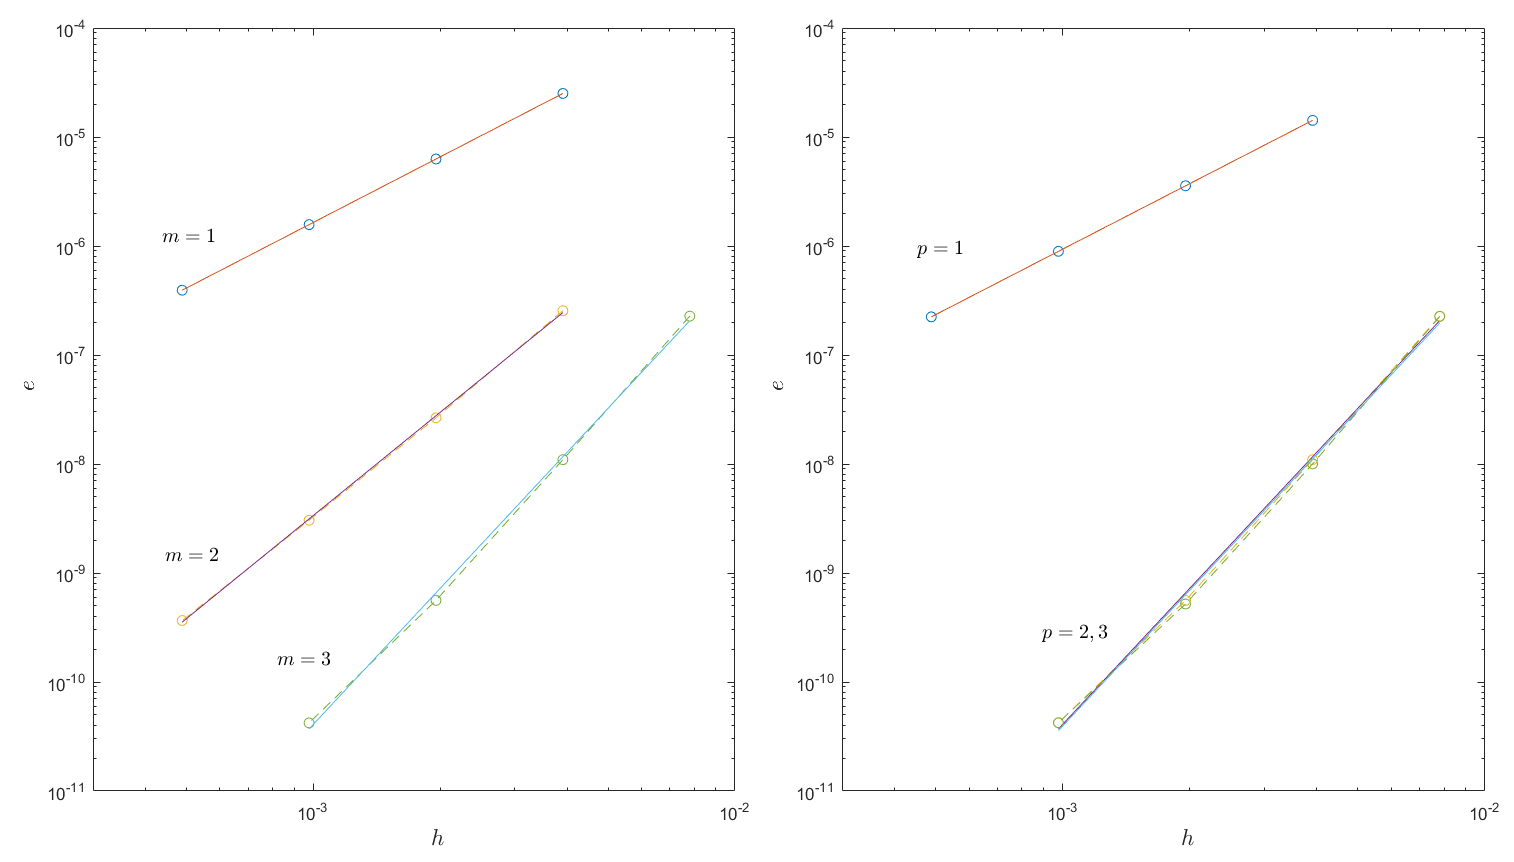
\includegraphics[width=0.95\textwidth]{Graphics/lldp-fj/mp_new.png}}
	\caption{Gráfico Log-log de error ${e_i=\max_{t_n\in(t)_{h_i}}\nnnorm{y_n-x(t_n)}_\infty}$ contra $h_i$ integrando la ecuación del Ejemplo \ref{ex:Brus} con el código \textit{JF-LLRK}, fijando $\eta_1=\eta_2=2$, $\alpha_1=\alpha_2$=0.5, $\beta=1$ y $h_i=2^{-i}$, $i=7,8,9,10,11$, y : Izquierda, $\mf=1,2,3$, $\pf=2$; y Derecha, $\pf=1,2,3$, $\mf=3$.} \label{Fig1}
\end{figure}

\begin{table}[htb]
	\centering
	\caption{
		Orden de convergencia $r$ del esquema (\ref{JFLLRK4}) y las estimaciones $\widetilde{r}$ para diferentes valores de $\mf$ y $\pf$, el intervalo de $90\%$ de confianza $[\widetilde{r}-\varDelta,\widetilde{r}+\varDelta]$, y el coeficiente de determinación $R^2$ de la recta ajustada en Figura \ref{Fig1}. Lo valores $\eta_1=\eta_2=2$, $\alpha_1=\alpha_2=0.5$ y $\beta=1$ se mantienen fijos.}
	\begin{adjustbox}{width=0.8\columnwidth,center}
		\begin{tabular}{cccccllccccc}
			\cline{1-12}
			&  & $\pf=2$ &  &  &  &  &  &  & $\mf=3$ &  &  \\ \cline{2-5}\cline{9-12}
			$\mf$ & $r$ & $\widetilde{r}$ & $\pm \varDelta$ & $R^{2}$ &  &  & $\pf+\pf$
			& $r$ & $\widetilde{r}$ & $\pm \varDelta$ & $R^{2}$ \\ 
			\cline{1-5}\cline{8-12}
			1 & 2 & 1.999 & 0.001 & 0.98 &  &  & 2 & 2 & 1.996 & 0.003 & 0.98 \\ 
			2 & 3 & 3.145 & 0.149 & 0.98 &  &  & 4 & 4 & 4.148 & 0.476 & 0.98 \\ 
			3 & 4 & 4.148 & 0.476 & 0.98 &  &  & 6 & 4 & 4.141 & 0.633 & 0.98 \\ 
			\cline{1-12}
		\end{tabular}
	\end{adjustbox}
	\label{tab:mporders}
\end{table}


Los errores $e_i=\max_{t_n\in(t)_{h_i}}\nnnorm{y_n-x(t_n)}_\infty$ del código \textit{JF-LLRK} en la integración de la ecuación de Brusselator fueron calculados para diferentes discretizaciones de tiempo $(t)_{h_i}$ con un tamaño de paso fijo $h_i$, donde la \textquotedblleft solución exacta\textquotedblright ~$x$ se estima mediante el código Matlab \textit{ode15s} con tolerancias $RTol= 10^{-12}$ y $ATol=10^{-14}$. La Figura \ref{Fig1}-izquierda muestra cuatro de estos errores para el código \textit{JF-LLRK} con diferentes valores de $\mf$, y fijo $\pf=2$, $\eta_1=\eta_2=2$ , $\alpha_1=\alpha_2=0.5$ y $\beta=1$, así como la recta ajustada a los puntos $(\log_2(h_i),\log_2(e_i))$ con $i=1,. ..,4$. La Tabla \ref{tab:mporders}-izquierda presenta el valor de la pendiente $\widetilde{r}$ de la línea recta ajustada para cada valor de $\mf$, lo que proporciona una estimación del orden de convergencia del esquema. La tabla también presenta el intervalo de $90\%$ de confianza $[\widetilde{r}-\varDelta,\widetilde{r}+\varDelta]$, el coeficiente de determinación $R^2$ como indicador de la bondad de ajuste de la línea recta, y el orden de convergencia esperado $r$ que - de acuerdo con el Teorema \ref {theorem:kp-fj-llrk-convergence} - el esquema (\ref{JFLLRK4}) tiene para los diferentes valores de $\mf$. La Figura \ref{Fig1}-derecha y la Tabla \ref{tab:mporders}-derecha presentan resultados similares pero para el código \textit{JF-LLRK} con varios valores de $\pf$ y $\mf=3$, $\eta_1=\eta_2=2$, $\alpha_1=\alpha_2=0.5$ y $\beta=1$. Observe que el orden de convergencia estimado $\widetilde{r}$ proporcionado en la Tabla \ref{tab:mporders} concuerda con el orden de convergencia del esquema (\ref{JFLLRK4}) establecido por el Teorema \ref{theorem:kp-fj-llrk-convergence} para los valores considerados de $\mf$ y $\pf$.

Análogamente, las Figuras \ref{Fig2}, \ref{Fig3} y las Tablas \ref{tab:out}, \ref{tab:in} presentan los resultados de las simulaciones correspondientes al orden de convergencia del esquema (\ref{JFLLRK4}) en función de los parámetros de sus dos aproximaciones libres de Jacobiano. Nuevamente el orden de convergencia estimado $\widetilde{r}$ proporcionado en las Tablas \ref{tab:in} y \ref{tab:out} concuerda con el orden de convergencia del esquema (\ref{JFLLRK4}) establecido por Teorema \ref{theorem:kp-fj-llrk-convergence} para los valores considerados de $\eta_1$, $\eta_2$, $\alpha_1$, $\alpha_2$ y $\beta$.


\begin{figure}[htb]
	\centering
	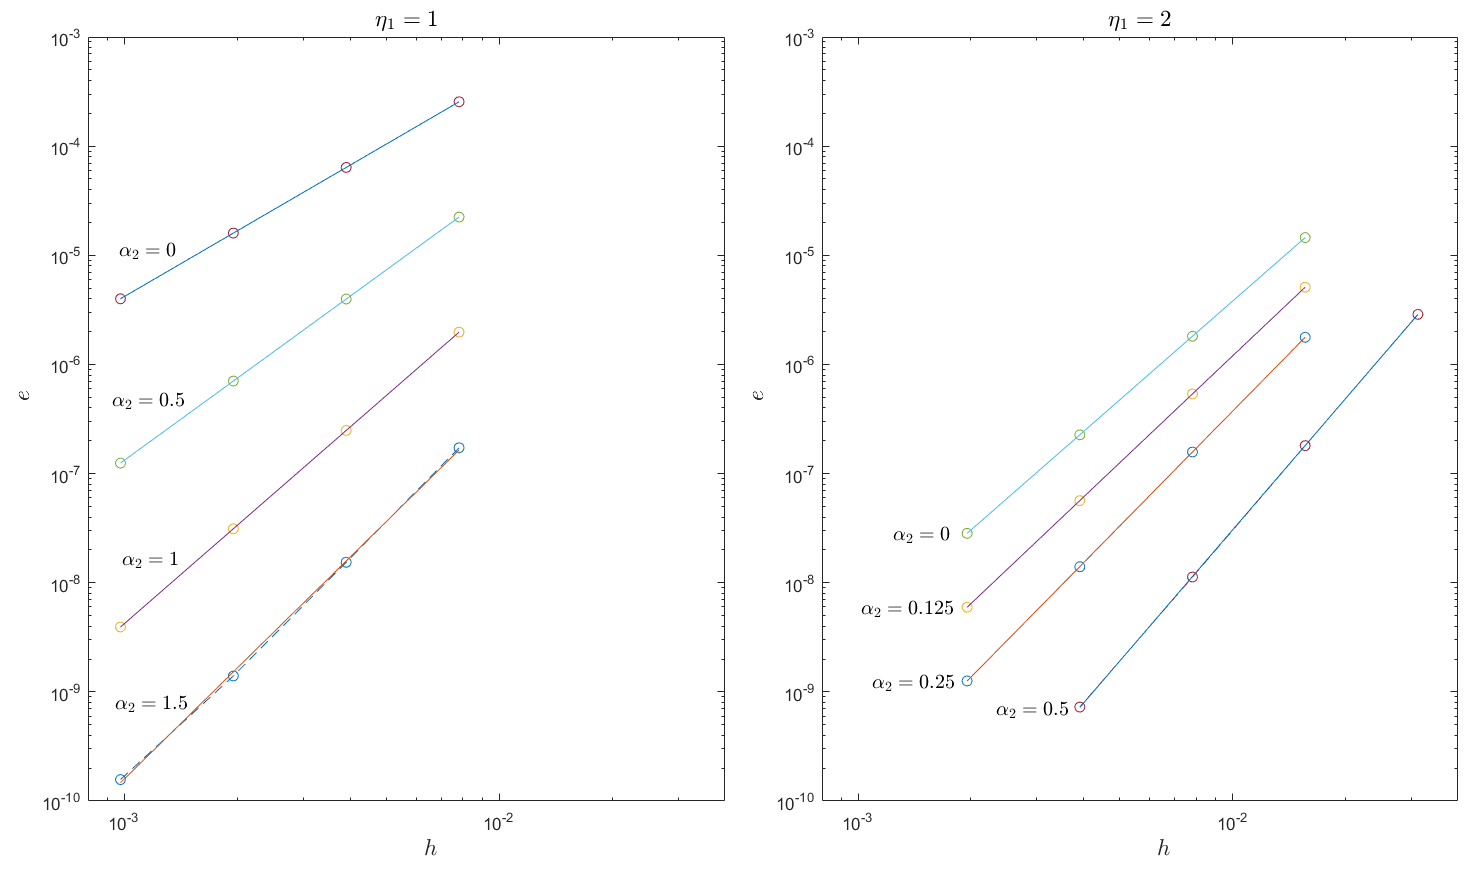
\includegraphics[width=0.95\textwidth]{Graphics/lldp-fj/out_new.png}
	\caption{Gráfico Log-log de error $e_i=\max_{t_n\in(t)_{h_i}}\nnnorm{y_n-x(t_n)}_\infty$ contra $h_i$ integrando la ecuación del Ejemplo \ref{ex:Brus} con el código \textit{JF-LLRK}, fijando $\mf=14$, $\pf=4$, $\eta_1=2$, $\alpha_1$=0.5, $\beta=1$, y: Izquierda, $\eta_2=1$, $\alpha_2$=0,0.5,1,1.5, $h_i=2^{-i}$, $i=7,8,9,10$ y Derecha, $\eta_2=2$, $\alpha_2$=0,0.125,0.25,0.5, $h_i=2^{-i}$, $i=5,6,7,8,9$.}
	\label{Fig2}
\end{figure}

\begin{table}[htb]
	\centering
	\caption{
		Orden de convergencia $r$ del esquema (\ref{JFLLRK4}) y las estimaciones $\widetilde{r}$ para diferentes valores de $\eta_2$ y $\alpha_2$, el intervalo de $90\%$ de confianza $[\widetilde{r}-\varDelta,\widetilde{r}+\varDelta]$, el coeficiente de determinación $R^2$ de la recta ajustada en Figura \ref{Fig2}. Los valores de $\mf=14$, $\pf=4$, $\eta_1=2$, $\alpha_1=0.5$ y $\beta=1$ se mantienen fijos. }
	\begin{adjustbox}{width=0.8\columnwidth,center}
		\begin{tabular}{ c  c c c c  c  c c c c c}
			\hline
			& \multicolumn{4}{c}{$\eta_2=1$} & & & \multicolumn{4}{c}{$\eta_2=2$} \\
			\cline{2-5} \cline{8-11}
			$\alpha_2$ & $r$ & $\widetilde{r}$ & $\pm\varDelta$ & $R^2$ & & $\alpha_2$ & $r$ & $\widetilde{r}$ & $\pm\varDelta$ & $R^2$ \\
			\hline
			0 & 2 & 1.999 & 0.001 & 0.98 & & 0 & 3 & 3.000 & 0.002 & 0.97 \\
			0.5 & 2.5 & 2.496 & 0.003 & 0.98 & & 0.125 & 3.25 & 3.247 & 0.003 & 0.97 \\
			1 & 3 & 2.992 & 0.005 & 0.98 & & 0.25 & 3.5 & 3.487 & 0.013 & 0.97 \\
			1.5 & 3.5 & 3.376 & 0.025 & 0.98 & & 0.5 & 4 & 3.986 & 0.029 & 0.97 \\
			\hline
		\end{tabular}
	\end{adjustbox}
	\label{tab:out}
\end{table}


\begin{figure}[htb]
	\centering
	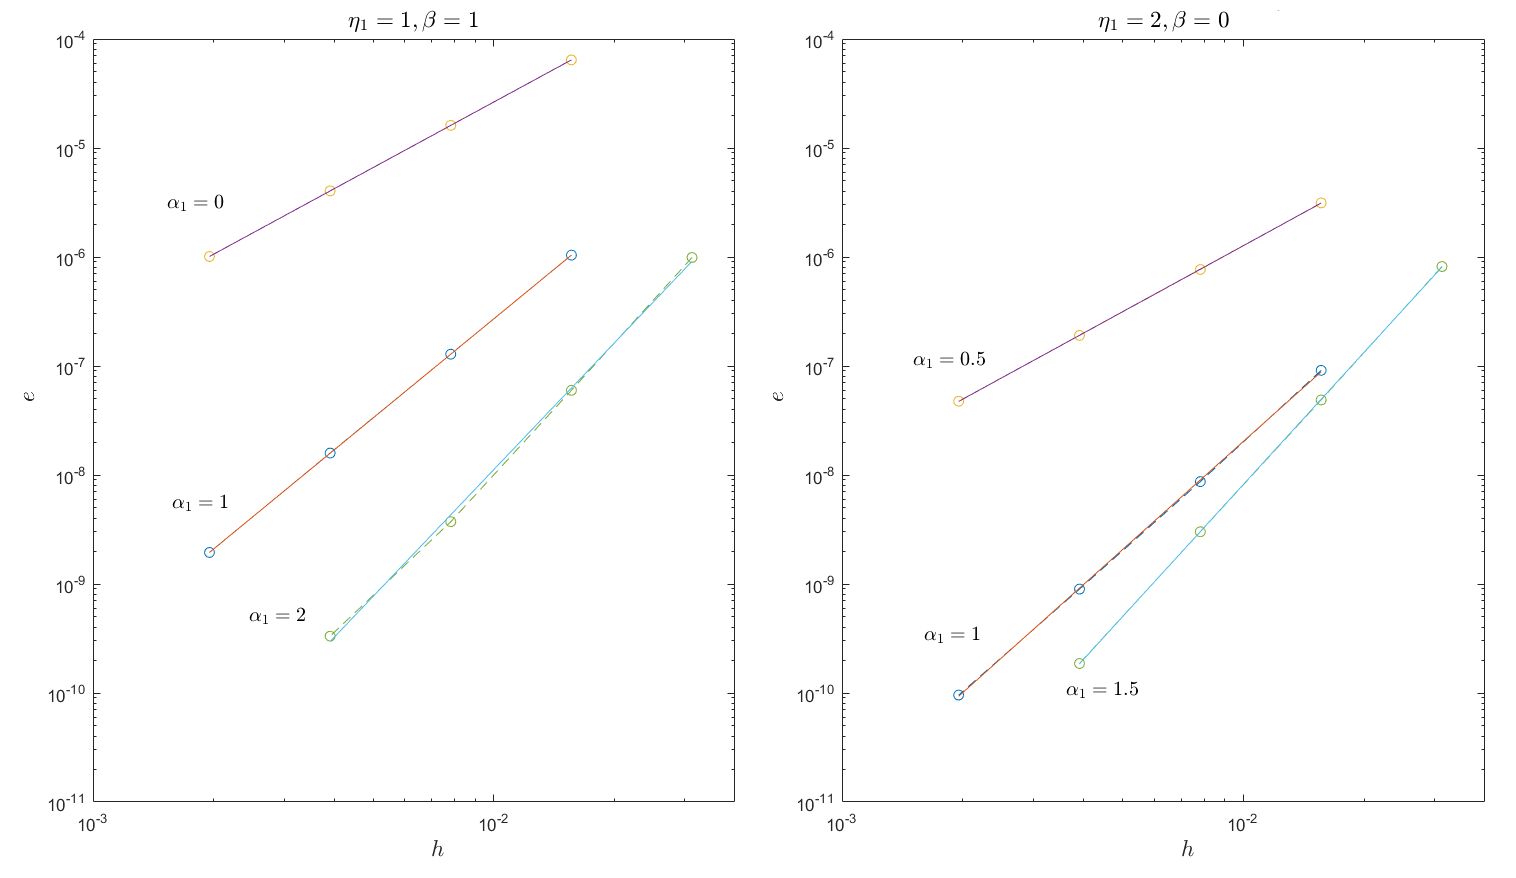
\includegraphics[width=0.95\textwidth]{Graphics/lldp-fj/in_new.png}
	\caption{Gráfico Log-log de error $e_i=\max_{t_n\in(t)_{h_i}}\nnnorm{y_n-x(t_n)}_\infty$ contra $h_i$ integrando la ecuación del Ejemplo \ref{ex:Brus} con el código \textit{JF-LLRK}, fijando $\mf=14$, $\pf=4$, $\eta_2=2$, $\alpha_2=1$, $h_i=2^{-i}$, $i=5,6,7,8,9$, y: Izquierda, $\alpha_1=0,1,2$ para $\eta_1=1,\beta=1$; Derecha, $\alpha_1$=0.5,1,1.5 para $\eta_1=2,\beta=0$.}
	\label{Fig3}
\end{figure}


\begin{table}[htb]
	\centering
	\caption{
        Orden de convergencia $r$ del esquema (\ref{JFLLRK4}) y las estimaciones $\widetilde{r}$ para diferentes valores de  $\eta_1$, $\alpha_1$ y $\beta$, el intervalo de $90\%$ de confianza $[\widetilde{r}-\varDelta,\widetilde{r}+\varDelta]$, el coeficiente de determinación $R^2$ de la recta ajustada en Figura \ref{Fig3}. Los valores de $\mf=14$, $\pf=4$, $\eta_2=2$ y$\alpha_2=1$ se mantienen fijos.}
	\begin{adjustbox}{width=0.8\columnwidth,center}
		\begin{tabular}{ccccccccccccc}
			\hline
			&  & \multicolumn{4}{c}{$\eta _{1}=1$} &  &  &  & \multicolumn{4}{c}{$\eta
				_{1}=2$} \\ \cline{3-6}\cline{10-13}
			$\beta $ & $\alpha _{1}$ & $r$ & $\widetilde{r}$ & $\pm \varDelta$ & $R^{2}$
			&  & $\beta $ & $\alpha _{1}$ & $r$ & $\widetilde{r}$ & $\pm \varDelta$ & $%
			R^{2}$ \\ \hline
			1 & 0 & 2 & 1.997 & 0.004 & 0.97 &  & 0 & 0.5 & 2 & 2.014 & 0.017 & 0.97 \\ 
			1 & 1 & 3 & 3.020 & 0.010 & 0.97 &  & 0 & 1 & 3 & 3.300 & 0.116 & 0.97 \\ 
			1 & 2 & 4 & 3.863 & 0.421 & 0.97 &  & 0 & 1.5 & 4 & 4.031 & 0.039 & 0.97 \\ 
			\hline
		\end{tabular}
	\end{adjustbox}
	\label{tab:in}
\end{table}

\subsubsection{Simulaciones comparativas}\label{sc:comparison}

En este conjunto de simulaciones, se utilizaron los PVI resultantes de la discretización espacial de cuatro EDP. Estas ecuaciones son: Brusselator 2D (Ejemplo \ref{ex:Brus}), Brusselator 2D (Ejemplo \ref{ex:Brus2D}), Burger's (Ejemplo \ref{ex:Burgers}) y Gray-Scott 2D~(Ejemplo \ref{ex:GS2D}).

Para cada ecuación de prueba, los resultados de la integración numérica se sintetizan en los diagramas de tiempo-precisión de la Figura \ref{work-precision diagram}. En estos diagramas, la precisión de los códigos \textit{JF-LLRK4}, \textit{JF-Exp4}, \textit{JF-EPIRK4} y \textit{BDF4} se mide por el error $e_i=\max\limits_ {t_n\in(t)_{h_i}}\nnnorm{y_n-x(t_n)}_\infty$ entre la \textquotedblleft solución exacta\textquotedblright~$x$ de la ecuación de prueba y la solución aproximada $y_n$ de cada código calculado en cinco particiones de tiempo con un tamaño de paso fijo $h_i$, donde la \textquotedblleft solución exacta\textquotedblright ~$x $ se estima nuevamente como en las simulaciones preliminares. La Figura \ref{work-precision diagram} muestra que, para estas ecuaciones, el esquema LLRK libre de Jacobiano (\ref{JFLLRK4}) exhibe una precisión similar o mayor que los otros tres integradores libres de Jacobiano, pero con un costo computacional menor o similar. Esta diferencia en el tiempo computacional se explica por los resultados de las Tablas \ref{tab:br}-\ref{tab:gs2d}.

\begin{figure}[htb]
	\centering
	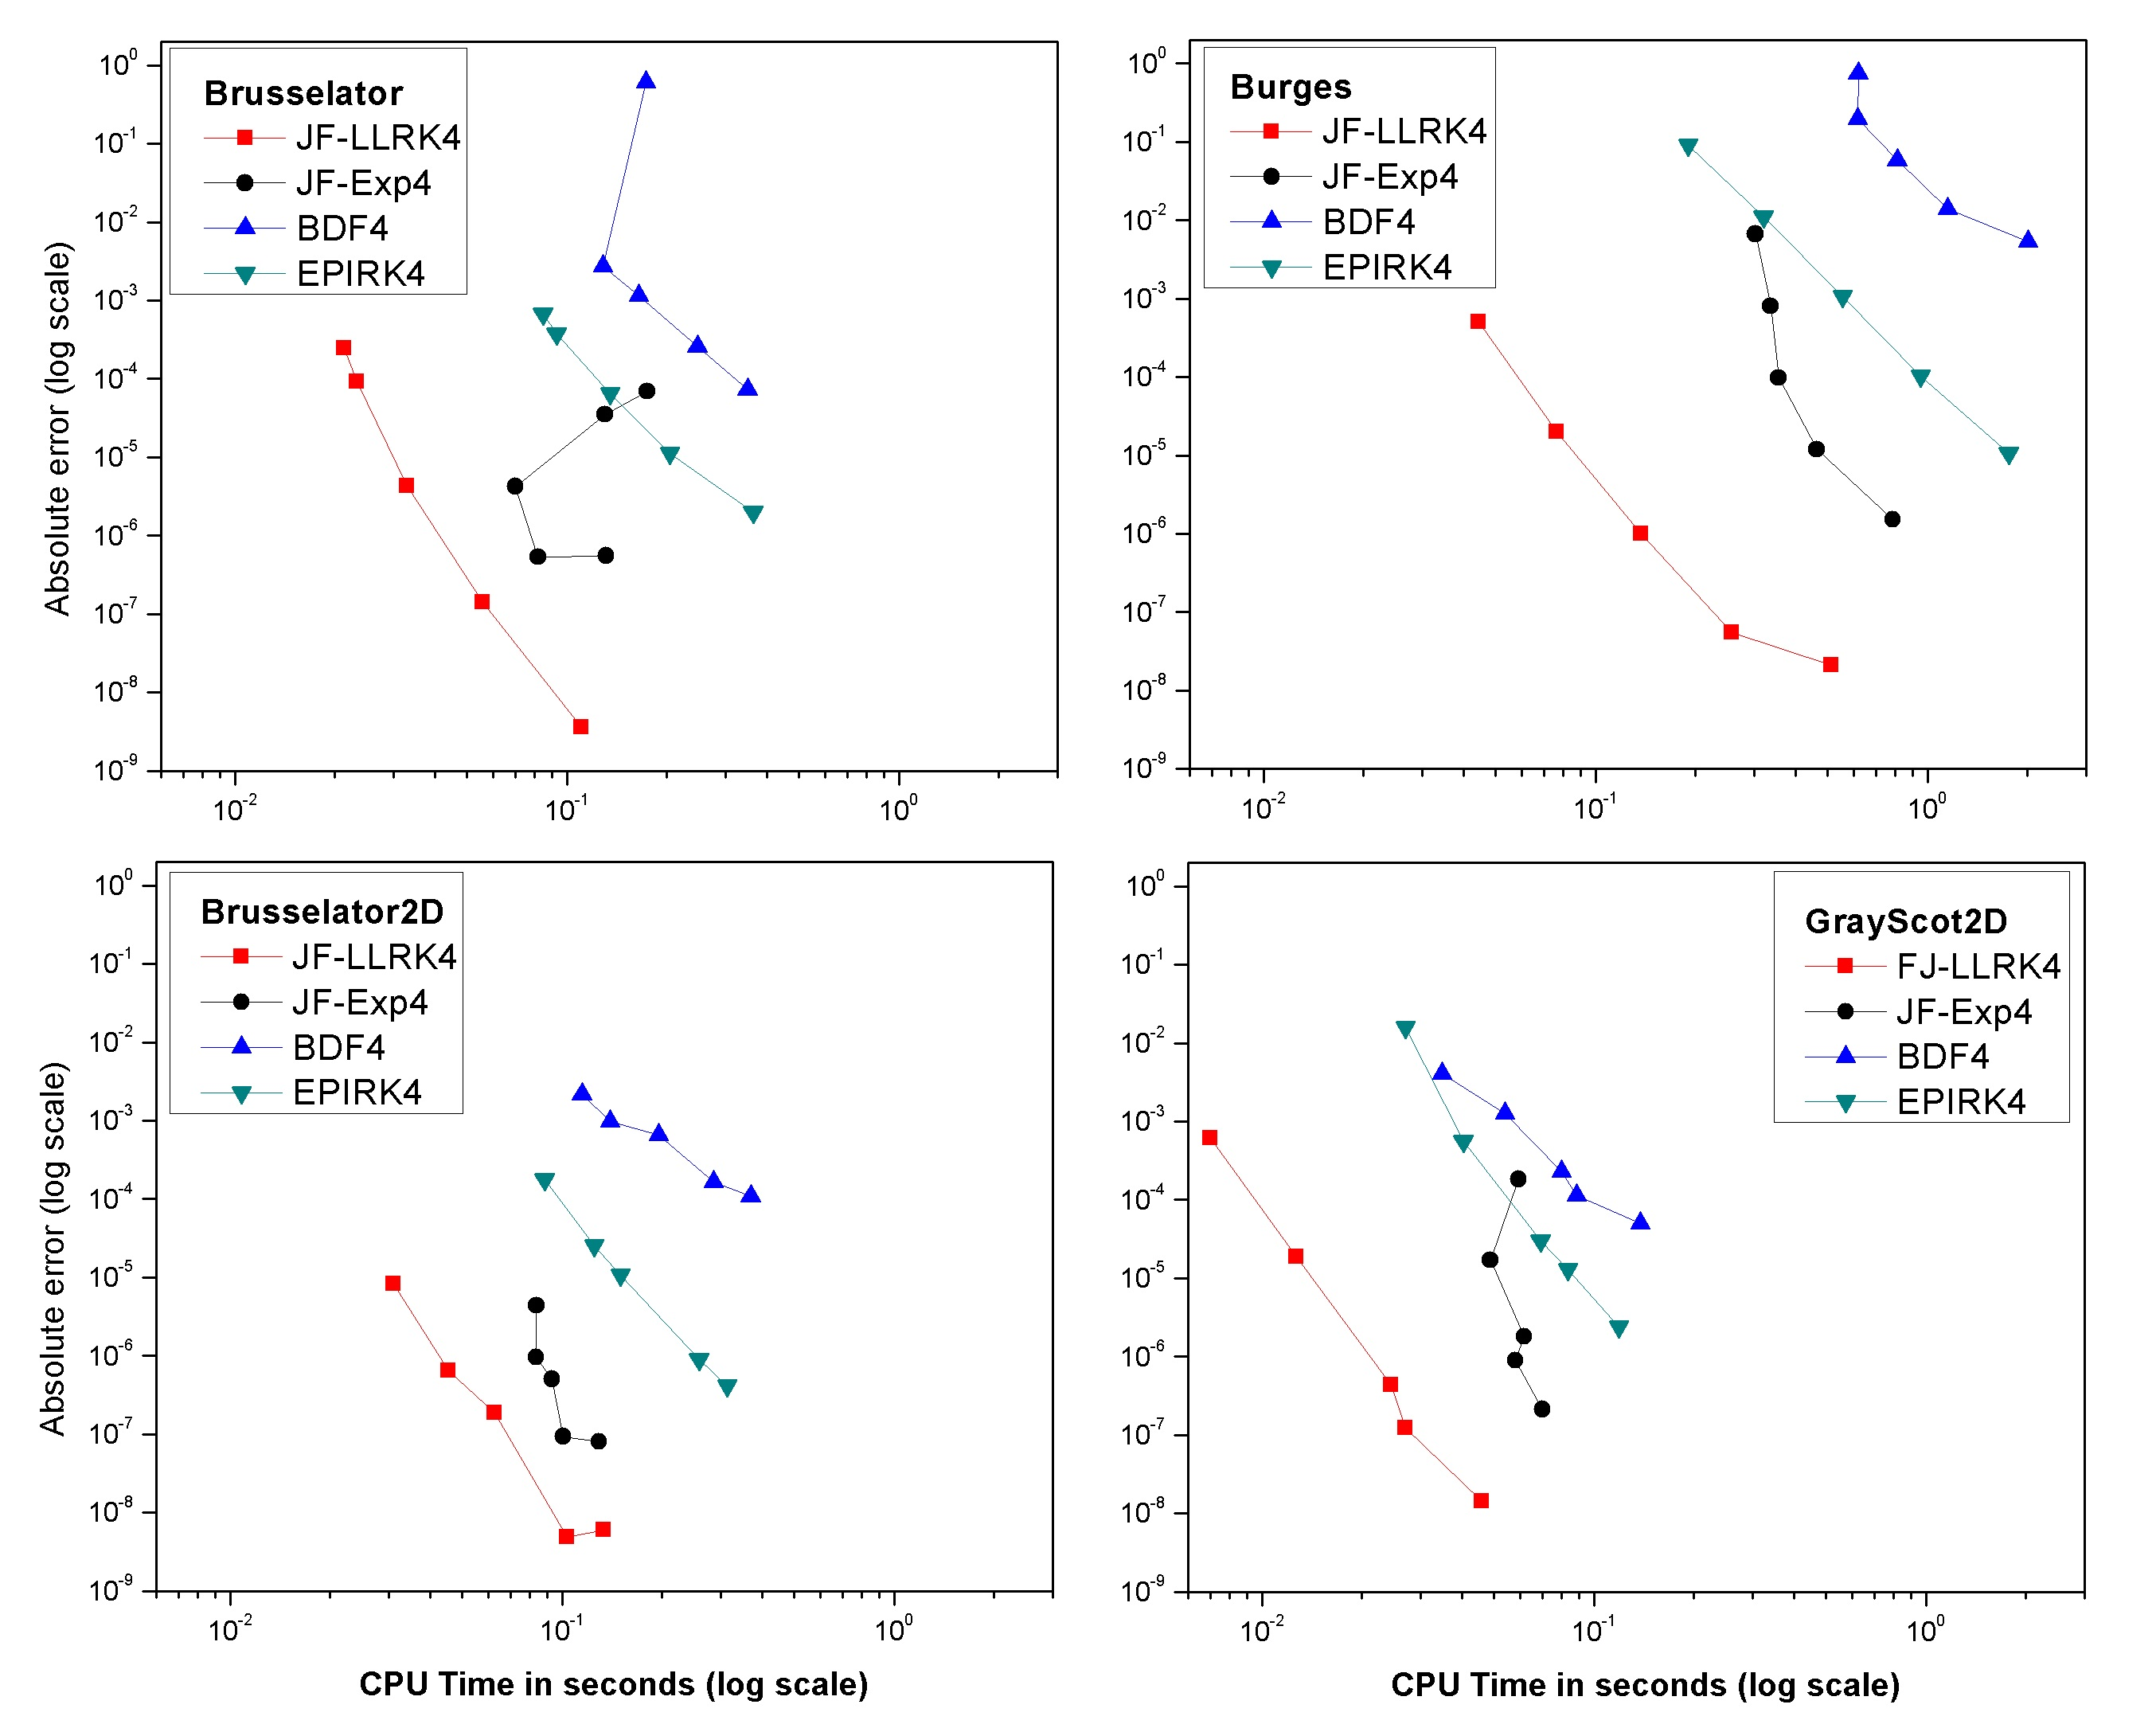
\includegraphics[width=1\textwidth]{Graphics/lldp-fj/Diagram_new.jpg}
	\caption{Diagramas comparativos de precisión contra tiempo en escala log-log para cada uno de los cuatro códigos de paso fijo en la integración de las cuatro ecuaciones de prueba. $\vartriangle$: código \emph{BDF4}, $\triangledown$: código \emph{JF-EPIRK4},  $\circ$ : código \emph{JF-Exp4}, y $\square$: código \emph{JF-LLRK4}} \label{work-precision diagram}
\end{figure}

Para cada código, las Tablas \ref{tab:br}-\ref{tab:gs2d} presentan el tamaño del paso \textit{h}, el número de pasos \textit{Pasos}, el número de evaluaciones del campo vectorial \textit{f-Eval}, el número de aproximaciones del subespacio Krylov \textit{K-subspace} a los productos de la función phi por un vector, el número de sistemas lineales en el código \textit{BDF4} resuelto por el método General Minimal Residue \textit {GMRES}, y el número de aproximaciones de Padé \textit{Padé} requeridas por los tres integradores exponenciales. Además, la dimensión mínima $\mf_{min}$, máxima $\mf_{max}$ y total $\mf_{total}$ de los subespacios de Krylov requerida por los códigos \textit{JF-LLRK4}, \textit{JF-Exp4} y \textit{JF-EPIRK4} para integrar las ecuaciones de prueba en todo el intervalo de integración también se especifica. Para el código \emph{BDF4}, $\mf_{min}$, $\mf_{max}$ y $\mf_{total}$ representan el número mínimo, máximo y total de iteraciones realizadas por el método GMRES sobre todo el intervalo de integración. En las tablas $d$ especifica el número de ecuaciones de cada ejemplo de prueba.

En cada paso de integración, al igual que para el esquema (5.8) de \cite{hochbruck1998exponential}, el código \textit{JF-Exp4} realiza tres descomposiciones en subespacios de Krylov y, al menos, tres aproximaciones (6,6)-Padé a la función $\varphi_1$ de las matrices de Hessenberg resultantes del Algoritmo de Arnoldi libre de Jacobiano \ref{alg:iArnoldi}. \textit{JF-Exp4} utiliza la diferencia hacia adelante de primer orden como una aproximación del producto de la matriz Jacobiana por un vector en el Algoritmo \ref{alg:iArnoldi}, lo cual reduce a tres el orden de convergencia del esquema (5.8) de \cite{hochbruck1998exponential} (ver Teorema 5.1 en \cite{hochbruck1998exponential}). Para estimar la dimensión de Krylov $\mf$, el código \textit{JF-Exp4} usa el algoritmo adaptativo de \cite{hochbruck1998exponential} y no hay restricción al valor mínimo para $\mf$.

El código \textit{JF-EPIRK4} requiere de las mismas descomposiciones de Krylov y un número similar de aproximaciones de Padé que el código \textit{JF-Exp4} en cada paso de integración, pero la dimensión de Krylov $\mf$ se estima automáticamente mediante el estrategia adaptativa de \cite{niesen2012algorithm} implementada en el código de Matlab \textit{phipm}.

Para resolver los sistemas algebraicos no lineales, en cada paso de integración, el código \textit{BDF4} emplea el método clásico de Newton junto con el método General Minimal Residue (GMRES) (función de Matlab \textit{gmres} con tolerancia $RTol=10^{-6}$) y la diferencia finita hacia adelante de primer orden como una aproximación al producto de la matriz Jacobiana por vector. En la función de Matlab \textit{gmres}, se eliminaron las comprobaciones computacionalmente costosas de las funciones de Matlab \textit{iterchk} y \textit{iterapp}.

\begin{table}[htb]
	\caption{Desempeño de los códigos de paso fijo \textit{JF-LLRK4}, \textit{JF-Exp4}, \textit{JF-EPIRK4} y \textit{BDF4} en la integración de la ecuación Brusselator con $M=100$, $d=200$.}
	\centering
	\begin{adjustbox}{width=0.9\columnwidth,center}
		\begin{tabular}{cccccccccc}
			\hline
			\textit{h} & Código & Pasos & f-Eval & K-subspace & GMRES & Padé & $\mf_{total}$ & $\mf%
			_{min}$ & $\mf_{max}$ \\ \hline
			\multicolumn{1}{l}{0.0250} & \multicolumn{1}{l}{JF-LLRK4} & 40 & 852 & 40 &
			0 & 40 & 492 & 4 & 16 \\
			\multicolumn{1}{l}{} & \multicolumn{1}{l}{JF-Exp4} & 40 & 3324 & 120 & 0 &
			1168 & 3124 & 4 & 48 \\
			\multicolumn{1}{l}{} & \multicolumn{1}{l}{BDF4} & 40 & 7318 & 0 & 400 & 0 &
			3305 & 3 & 24 \\
			\multicolumn{1}{l}{} & \multicolumn{1}{l}{JF-EPIRK4} & 40 & 1238 & 120 & 0 &
			625 & 718 & 4 & 11 \\
			\multicolumn{1}{l}{0.0200} & \multicolumn{1}{l}{JF-LLRK4} & 50 & 967 & 50 &
			0 & 50 & 517 & 4 & 13 \\
			\multicolumn{1}{l}{} & \multicolumn{1}{l}{JF-Exp4} & 50 & 2855 & 150 & 0 &
			1147 & 2605 & 4 & 48 \\
			\multicolumn{1}{l}{} & \multicolumn{1}{l}{BDF4} & 50 & 7156 & 0 & 448 & 0 &
			2780 & 2 & 23 \\
			\multicolumn{1}{l}{} & \multicolumn{1}{l}{JF-EPIRK4} & 50 & 1425 & 150 & 0 &
			716 & 775 & 3 & 10 \\
			\multicolumn{1}{l}{0.0100} & \multicolumn{1}{l}{JF-LLRK4} & 100 & 1477 & 100
			& 0 & 100 & 577 & 4 & 10 \\
			\multicolumn{1}{l}{} & \multicolumn{1}{l}{JF-Exp4} & 100 & 1773 & 300 & 0 &
			970 & 1273 & 2 & 36 \\
			\multicolumn{1}{l}{} & \multicolumn{1}{l}{BDF4} & 100 & 6574 & 0 & 476 & 0 &
			2269 & 2 & 13 \\
			\multicolumn{1}{l}{} & \multicolumn{1}{l}{JF-EPIRK4} & 100 & 2278 & 300 & 0 &
			976 & 978 & 2 & 7 \\
			\multicolumn{1}{l}{0.0050} & \multicolumn{1}{l}{JF-LLRK4} & 200 & 2609 & 200
			& 0 & 200 & 809 & 4 & 6 \\
			\multicolumn{1}{l}{} & \multicolumn{1}{l}{JF-Exp4} & 200 & 2256 & 600 & 0 &
			1242 & 1256 & 1 & 15 \\
			\multicolumn{1}{l}{} & \multicolumn{1}{l}{BDF4} & 200 & 7055 & 0 & 588 & 0 &
			2678 & 1 & 12 \\
			\multicolumn{1}{l}{} & \multicolumn{1}{l}{JF-EPIRK4} & 200 & 3894 & 600 & 0 &
			1294 & 1294 & 1 & 5 \\
			\multicolumn{1}{l}{0.0025} & \multicolumn{1}{l}{JF-LLRK4} & 400 & 5201 & 400
			& 0 & 400 & 1601 & 4 & 5 \\
			\multicolumn{1}{l}{} & \multicolumn{1}{l}{JF-Exp4} & 400 & 3945 & 1200 & 0 &
			1945 & 1945 & 1 & 4 \\
			\multicolumn{1}{l}{} & \multicolumn{1}{l}{BDF4} & 400 & 9530 & 0 & 919 & 0 &
			3556 & 1 & 10 \\
			\multicolumn{1}{l}{} & \multicolumn{1}{l}{JF-EPIRK4} & 400 & 7287 & 1200 & 0 &
			2087 & 2087 & 1 & 3 \\
			\hline
		\end{tabular}
	\end{adjustbox}
	\label{tab:br}
\end{table}



\begin{table}[htb]
	\caption{Desempeño de los códigos de paso fijo \textit{JF-LLRK4}, \textit{JF-Exp4}, \textit{JF-EPIRK4} y \textit{BDF4} en la integración de la ecuación Brusselator 2D con $M=40$, $d=3200$.}
	\centering
	\begin{adjustbox}{width=0.9\columnwidth,center}
		\begin{tabular}{cccccccccc}
			\hline
			\textit{h} & Código & Pasos & f-Eval & K-subspace & GMRES & Padé & $\mf_{total}$ & $\mf%
			_{min}$ & $\mf_{max}$ \\ \hline
			\multicolumn{1}{l}{0.01000} & \multicolumn{1}{l}{JF-LLRK4} & 10 & 144 & 10
			& 0 & 10 & 54 & 4 & 8 \\
			\multicolumn{1}{l}{} & \multicolumn{1}{l}{JF-Exp4} & 10 & 251 & 30 & 0 & 139
			& 201 & 2 & 20 \\
			\multicolumn{1}{l}{} & \multicolumn{1}{l}{BDF4} & 10 & 1243 & 0 & 86 & 0 &
			283 & 2 & 8 \\
			\multicolumn{1}{l}{} & \multicolumn{1}{l}{JF-EPIRK4} & 10 & 263 & 30 & 0 &
			129 & 133 & 3 & 6 \\
			\multicolumn{1}{l}{0.00625} & \multicolumn{1}{l}{JF-LLRK4} & 16 & 218 & 16
			& 0 & 16 & 74 & 4 & 6 \\
			\multicolumn{1}{l}{} & \multicolumn{1}{l}{JF-Exp4} & 16 & 284 & 48 & 0 & 167
			& 204 & 2 & 15 \\
			\multicolumn{1}{l}{} & \multicolumn{1}{l}{BDF4} & 16 & 1618 & 0 & 118 & 0 &
			334 & 1 & 7 \\
			\multicolumn{1}{l}{} & \multicolumn{1}{l}{JF-EPIRK4} & 16 & 383 & 48 & 0 &
			174 & 175 & 2 & 6 \\
			\multicolumn{1}{l}{0.00500} & \multicolumn{1}{l}{JF-LLRK4} & 20 & 268 & 20 &
			0 & 20 & 88 & 4 & 6 \\
			\multicolumn{1}{l}{} & \multicolumn{1}{l}{JF-Exp4} & 20 & 307 & 60 & 0 & 184
			& 207 & 2 & 15 \\
			\multicolumn{1}{l}{} & \multicolumn{1}{l}{BDF4} & 20 & 1449 & 0 & 109 & 0 &
			313 & 1 & 6 \\
			\multicolumn{1}{l}{} & \multicolumn{1}{l}{JF-EPIRK4} & 20 & 464 & 60 & 0 &
			204 & 204 & 2 & 5 \\
			\multicolumn{1}{l}{0.00250} & \multicolumn{1}{l}{JF-LLRK4} & 40 & 521 & 40 &
			0 & 40 & 161 & 4 & 5 \\
			\multicolumn{1}{l}{} & \multicolumn{1}{l}{JF-Exp4} & 40 & 455 & 120 & 0 & 251
			& 255 & 1 & 8 \\
			\multicolumn{1}{l}{} & \multicolumn{1}{l}{BDF4} & 40 & 1452 & 0 & 120 & 0 &
			384 & 1 & 5 \\
			\multicolumn{1}{l}{} & \multicolumn{1}{l}{JF-EPIRK4} & 40 & 846 & 120 & 0 &
			326 & 326 & 1 & 4 \\
			\multicolumn{1}{l}{0.00200} & \multicolumn{1}{l}{JF-LLRK4} & 50 & 650 & 50
			& 0 & 50 & 200 & 4 & 4 \\
			\multicolumn{1}{l}{} & \multicolumn{1}{l}{JF-Exp4} & 50 & 541 & 150 & 0 & 289
			& 291 & 1 & 8 \\
			\multicolumn{1}{l}{} & \multicolumn{1}{l}{BDF4} & 50 & 1785 & 0 & 150 & 0 &
			457 & 1 & 5 \\
			\multicolumn{1}{l}{} & \multicolumn{1}{l}{JF-EPIRK4} & 50 & 1027 & 150 & 0 &
			377 & 377 & 1 & 4 \\
			\hline
		\end{tabular}
	\end{adjustbox}
	\label{tab:br2d}
\end{table}

\begin{table}[htb]
	\caption{Desempeño de los códigos de paso fijo \textit{JF-LLRK4}, \textit{JF-Exp4}, \textit{JF-EPIRK4} y \textit{BDF4} en la integración de la ecuación Burger's con $M=400$, $d=400$.}
	\centering
	\begin{adjustbox}{width=0.9\columnwidth,center}
		\begin{tabular}{cccccccccc}
			\hline
			\textit{h} & Código & Pasos & f-Eval & K-subspace & GMRES & Padé & $\mf_{total}$ & $\mf%
			_{min}$ & $\mf_{max}$ \\ \hline
			\multicolumn{1}{l}{0.0050000} & \multicolumn{1}{l}{JF-LLRK4} & 100 & 1614 &
			100 & 0 & 100 & 714 & 4 & 10 \\
			\multicolumn{1}{l}{} & \multicolumn{1}{l}{JF-Exp4} & 100 & 6104 & 300 & 0 &
			2507 & 5604 & 3 & 27 \\
			\multicolumn{1}{l}{} & \multicolumn{1}{l}{BDF4} & 100 & 17304 & 0 & 910 & 0
			& 6469 & 2 & 12 \\
			\multicolumn{1}{l}{} & \multicolumn{1}{l}{JF-EPIRK4} & 100 & 2874 & 300 & 0 &
			1435 & 1574 & 3 & 7 \\
			\multicolumn{1}{l}{0.0025000} & \multicolumn{1}{l}{JF-LLRK4} & 200 & 2922 &
			200 & 0 & 200 & 1122 & 4 & 8 \\
			\multicolumn{1}{l}{} & \multicolumn{1}{l}{JF-Exp4} & 200 & 7287 & 600 & 0 &
			3784 & 6287 & 2 & 20 \\
			\multicolumn{1}{l}{} & \multicolumn{1}{l}{BDF4} & 200 & 27333 & 0 & 1665 & 0
			& 7783 & 2 & 10 \\
			\multicolumn{1}{l}{} & \multicolumn{1}{l}{JF-EPIRK4} & 200 & 4988 & 600 & 0 &
			2388 & 2388 & 2 & 5 \\
			\multicolumn{1}{l}{0.0012500} & \multicolumn{1}{l}{JF-LLRK4} & 400 & 5361 &
			400 & 0 & 400 & 1761 & 4 & 5 \\
			\multicolumn{1}{l}{} & \multicolumn{1}{l}{JF-Exp4} & 400 & 8123 & 1200 & 0 &
			4975 & 6123 & 1 & 11 \\
			\multicolumn{1}{l}{} & \multicolumn{1}{l}{BDF4} & 400 & 37402 & 0 & 2454 & 0
			& 9416 & 2 & 10 \\
			\multicolumn{1}{l}{} & \multicolumn{1}{l}{JF-EPIRK4} & 400 & 9111 & 1200 & 0 &
			3911 & 3911 & 1 & 4 \\
			\multicolumn{1}{l}{0.0006250} & \multicolumn{1}{l}{JF-LLRK4} & 800 & 10400 &
			800 & 0 & 800 & 3200 & 4 & 4 \\
			\multicolumn{1}{l}{} & \multicolumn{1}{l}{JF-Exp4} & 800 & 11223 & 2400 & 0
			& 7039 & 7223 & 1 & 8 \\
			\multicolumn{1}{l}{} & \multicolumn{1}{l}{BDF4} & 800 & 32269 & 0 & 2251 & 0
			& 8838 & 2 & 5 \\
			\multicolumn{1}{l}{} & \multicolumn{1}{l}{JF-EPIRK4} & 800 & 16766 & 2400 & 0 &
			6366 & 6366 & 1 & 4 \\
			\multicolumn{1}{l}{0.0003125} & \multicolumn{1}{l}{JF-LLRK4} & 1600 & 20800
			& 1600 & 0 & 1600 & 6400 & 4 & 4 \\
			\multicolumn{1}{l}{} & \multicolumn{1}{l}{JF-Exp4} & 1600 & 19555 & 4800 & 0
			& 11555 & 11555 & 1 & 4 \\
			\multicolumn{1}{l}{} & \multicolumn{1}{l}{BDF4} & 1600 & 58643 & 0 & 4360 & 0
			& 17910 & 2 & 8 \\
			\multicolumn{1}{l}{} & \multicolumn{1}{l}{JF-EPIRK4} & 1600 & 31872 & 4800 & 0 &
			11072 & 11072 & 1 & 3 \\
			\hline
		\end{tabular}
	\end{adjustbox}
	\label{tab:bg}
\end{table}


\begin{table}[htb]
	\caption{Desempeño de los códigos de paso fijo \textit{JF-LLRK4}, \textit{JF-Exp4}, \textit{JF-EPIRK4} y \textit{BDF4} en la integración de la ecuación Gray-Scott 2D con $M=20$, $d=800$.}
	\centering
	\begin{adjustbox}{width=0.9\columnwidth,center}
		\begin{tabular}{cccccccccc}
			\hline
			\textit{h} & Código & Pasos & f-Eval & K-subspace & GMRES & Padé & $\mf_{total}$ & $\mf%
			_{min}$ & $\mf_{max}$ \\ \hline
			0.010000 & \multicolumn{1}{l}{JF-LLRK4} & 10 & 161 & 10 & 0 & 10 & 71 & 4 &
			10 \\
			& \multicolumn{1}{l}{JF-Exp4} & 10 & 656 & 30 & 0 & 258 & 606 & 4 & 36 \\
			& \multicolumn{1}{l}{BDF4} & 10 & 923 & 0 & 52 & 0 & 332 & 2 & 14 \\
			& \multicolumn{1}{l}{JF-EPIRK4} & 10 & 296 & 30 & 0 & 148 & 166 & 4 & 9 \\
			0.005000 & \multicolumn{1}{l}{JF-LLRK4} & 20 & 296 & 20 & 0 & 20 & 116 & 4 &
			8 \\
			& \multicolumn{1}{l}{JF-Exp4} & 20 & 643 & 60 & 0 & 327 & 543 & 2 & 27 \\
			& \multicolumn{1}{l}{BDF4} & 20 & 1064 & 0 & 72 & 0 & 371 & 1 & 10 \\
			& \multicolumn{1}{l}{JF-EPIRK4} & 20 & 494 & 60 & 0 & 228 & 234 & 2 & 7 \\
			0.002500 & \multicolumn{1}{l}{JF-LLRK4} & 40 & 547 & 40 & 0 & 40 & 187 & 4 &
			8 \\
			& \multicolumn{1}{l}{JF-Exp4} & 40 & 787 & 120 & 0 & 439 & 587 & 1 & 20 \\
			& \multicolumn{1}{l}{BDF4} & 40 & 1308 & 0 & 101 & 0 & 468 & 2 & 7 \\
			& \multicolumn{1}{l}{JF-EPIRK4} & 40 & 889 & 120 & 0 & 369 & 369 & 1 & 5 \\
			0.002000 & \multicolumn{1}{l}{JF-LLRK4} & 50 & 669 & 50 & 0 & 50 & 219 & 4 &
			6 \\
			& \multicolumn{1}{l}{JF-Exp4} & 50 & 876 & 150 & 0 & 488 & 626 & 1 & 15 \\
			& \multicolumn{1}{l}{BDF4} & 50 & 1472 & 0 & 118 & 0 & 528 & 2 & 7 \\
			& \multicolumn{1}{l}{JF-EPIRK4} & 50 & 1079 & 150 & 0 & 429 & 429 & 1 & 5 \\
			0.001250 & \multicolumn{1}{l}{JF-LLRK4} & 80 & 1050 & 80 & 0 & 80 & 330 & 4
			& 6 \\
			& \multicolumn{1}{l}{JF-Exp4} & 80 & 1118 & 240 & 0 & 619 & 718 & 1 & 15 \\
			& \multicolumn{1}{l}{BDF4} & 80 & 2151 & 0 & 184 & 0 & 715 & 1 & 6 \\
			& \multicolumn{1}{l}{JF-EPIRK4} & 80 & 1626 & 240 & 0 & 586 & 586 & 1 & 4 \\
			\hline
		\end{tabular}
	\end{adjustbox}
	\label{tab:gs2d}
\end{table}


Se puede observar de las Tablas \ref{tab:br}-\ref{tab:gs2d}, que el código \textit{BDF4} requiere de un número mucho mayor de evaluaciones del campo vectorial que los otros tres códigos, lo que explica su mayor costo computacional en los diagramas tiempo-precisión de la Figura \ref{work-precision diagram}. Por otro lado, para los tamaños de paso más grandes, el número de evaluaciones del campo vectorial de los códigos \textit{JF-Exp4} y \textit{JF-EPIRK4} es mayor que el del código \textit{JF-LLRK4}, por lo que su costo computacional es mucho mayor que el del código \textit{JF-LLRK4}. Para los tamaños de paso más pequeños, el número de evaluaciones del campo vectorial del código \textit{JF-Exp4} es ligeramente inferior o similar al del código \textit{JF-LLRK4}, lo que explica el costo computacional similar de estos dos códigos en los diagramas tiempo-precisión correspondientes a las ecuaciones Brusselator y Brusselator 2D de la Figura \ref{work-precision diagram}.

Además, las Tablas \ref{tab:br}-\ref{tab:gs2d} muestran la efectividad de la estrategia del código \textit{JF-LLRK4} para la selección de la dimensión Krylov $\mf$ en cada paso de integración, con mínima variación entre los valores de $\mf_{min}$ y $\mf_{max}$, y por tanto, con un valor de $\mf_{total}$ mucho menor que los demás códigos.

En resumen, las simulaciones han demostrado que, con un costo computacional similar, el nuevo integrador libre de Jacobiano presenta una precisión mucho mayor que los otros tres integradores libres de Jacobiano; mientras que, con una precisión similar, el primero es mucho más rápido que los segundos.

Para concluir esta sección, recordemos que la selección de $\delta$ y $h$ en esquemas prácticos libres de Jacobiano se realiza bajo diferentes criterios que resultan en valores óptimos para $\delta$ y $h$ independientes entre sí \cite{knoll2004jacobian}. Con este conocimiento en mente, la teoría desarrollada hasta este punto y los experimentos numéricos realizados con $\delta$ vinculados a una potencia de $h$ pretenden sentar las bases para diseñar esquemas prácticos Localmente Linealizados de Orden Superior Libres Jacobiano con valores óptimos de $h$ y $\delta$.

\section{Esquema Runge-Kutta de Dormand y Prince Localmente Linealizado}
En ésta sección, se combinan las aproximaciones Krylov-Padé libre de Jacobiano del Capítulo \ref{chapter:solve-non-smal-lineal-eq} con las fórmulas embebidas Runge-Kutta de Dormand y Prince Localmente Linealizadas para implementar un esquema adaptativo de orden variable libre de Jacobiano.
\importantdefinition{Fórmulas embebidas Runge-Kutta de Dormand y Prince Localmente Linealizadas y libres de Jacobiano}
Utilizando la aproximación $(\mf , \pf ,\qf , k)$-Krylov-Padé Libre de Jacobiano
\begin{equation}
\widetilde{u}_j=\widehat{K}_{\mf,k}^{\pf,\qf}\left(c_j h_n, f_x(y_n) , f(y_n); \eta_1, \delta_1, \beta \right) \label{eq:approx_u_j},
\end{equation}
definida en (\ref{eq:gen_kp_aprox_fj}), para las $u_j$ en las fórmulas embebidas (\ref{lldis}) y las aproximaciones libres de Jacobiano $g_2(y_n,\widetilde{u}_j;\delta_2)$ al producto  $f_x(y_n)\widetilde{u}_j$ en (\ref{lldis}), obtenemos las fórmulas embebidas Runge-Kutta de Dormand y Prince Localmente Linealizadas y libres de Jacobiano
\begin{equation}
	y_{n+1}\,=\,y_n+\widetilde{u}_s+h_n \sum_{j=1}^{s}b_j \widetilde{\kt}_j \,\,\, \text{y} \,\,\, \
	\widehat{y}_{n+1}\,=\, y_n+\widetilde{u}_s+h_n \sum_{j=1}^{s}\widehat{b}_j \widetilde{\kt}_j, \label{Jacobian-free LLDPK scheme}
	\end{equation}
para integrar PVI de dimensiones no pequeñas, donde
\begin{equation*}
	\widetilde{\kt}_j = f\left( y_n+\widetilde{u}_j+h_n \sum_{i=1}^{j-1}a_{j,i}\widetilde{\kt}_i \right) - f( y_n) - g_2(y_n,\widetilde{u}_j;\delta_2),
\end{equation*}
y $\widetilde{\kt}_1=0$, son $a_{j,i}$, $b_j$, $\widehat{b}_j$ los coeficientes Runge-Kutta de Dormand y Prince definidos en la Tabla \ref{ButcherTabla} y  $g_2(y_n,\widetilde{u}_j;\delta_2)$ es la aproximación de $f_x(y_n)\widetilde{u}_j$ que satisface la cota~(\ref{eq:g_bound2}).

El siguiente teorema trata sobre la velocidad de convergencia de las fórmulas embebidas (\ref{Jacobian-free LLDPK scheme}). Con este propósito, estas fórmulas se reescriben como
\begin{equation*}
    y_{n+1}=y_{n}+\digamma (y_{n};h_{n})\text{ \ \ \ \ y \ \ \ \ }\widehat{y}_{n+1}=y_{n}+\widehat{\digamma }(y_{n};h_{n}).
\end{equation*}


\begin{theorem}\label{Teorema Convergencia}
	\cite{naranjo2022RT}~Sea $x$ solución de del PVI (\ref{ODE-SYST}) con campo vectorial $f$ seis veces continuamente diferenciable en el compacto $\mathfrak{K} \subset \mathfrak{D}$. Entonces, las fórmulas embebidas Runge-Kutta de Dormand y Prince Localmente Linealizadas y libres de Jacobiano (\ref{Jacobian-free LLDPK scheme}) tienen error de truncamiento local
	\[	\lvert\lvert x(t_{n+1}) - x(t_n) - \digamma(x(t_n);h_n) \rvert\rvert_2 \leq \mathfrak{c}_0h_n^{\min\{5,\mf+1,\pf+\qf \}+1} + \mathfrak{c}_1h_n^{\beta\eta_1+2}\delta_1^{\eta_1} + \mathfrak{c}_2h_n^{\eta_2+2}\delta_2^{\eta_2},
	\]
	\[	\lvert\lvert x(t_{n+1}) - x(t_n) - \widehat{\digamma }(x(t_n);h_n) \rvert\rvert_2 \leq \mathfrak{c}_0h_n^{\min\{4,\mf+1,\pf+\qf \}+1} + \mathfrak{c}_1h_n^{\beta\eta_1+2}\delta_1^{\eta_1} + \mathfrak{c}_2h_n^{\eta_2+2}\delta_2^{\eta_2},
	\]
	donde $\eta_1$ es el orden de la aproximación $g_1(.;\delta_1)$ en el Algoritmo de Arnoldi libre de Jacobiano \ref{alg:iArnoldi} para el $\mf$-ésimo subespacio de Krylov $\widehat{\mathcal{K}}_\mf(h^\beta f_x(x(t_n)),f(x(t_n));\delta_1)$, $\eta_2$ es el orden de la aproximación $g_2(.;\delta_2)$ en (\ref{Jacobian-free LLDPK scheme}), y $\mathfrak{c}_0,\mathfrak{c}_1,\mathfrak{c}_2$ son constantes positivas. Además, con $\delta_1\propto h^{\alpha_1}$, $\delta_2\propto h^{\alpha_2}$, $\alpha_1,\alpha_2 \geq 0$, el error global satisface
	\[ \lvert\lvert x(t_{n+1}) - y_{n+1} \rvert\rvert_2 \leq M h^{\mathrm{min}\left\{5,\mf+1,\pf+\qf,(\beta+\alpha_1)\eta_1+1,(1+\alpha_2)\eta_2+1 \right\}} \]
	\[ \lvert\lvert x(t_{n+1}) - \widehat{y}_{n+1} \rvert\rvert_2 \leq M h^{\mathrm{min}\left\{4,\mf+1,\pf+\qf,(\beta+\alpha_1)\eta_1+1,(1+\alpha_2)\eta_2+1 \right\}} \]
	para todo $t_{n+1},t_n\in(t)_h$ y $h$ suficiente pequeña, donde $M$ es una constante positiva.
\end{theorem}

\textbf{Demostración}
Los errores locales y globales para las fórmulas embebidas libres de Jacobiano (\ref{Jacobian-free LLDPK scheme}) se derivan directamente del Teorema \ref{theorem:kp-fj-llrk-convergence}, teniendo en cuenta que los errores de truncamiento locales de las fórmulas embebidas originales de Dormand y Prince son 6 y 5 \cite{hairer1993solving}.
$\Box$

En la práctica, similarmente a como se hizo en el Capítulo \ref{chapter:lldp}, las cinco aproximaciones (\ref{eq:approx_u_j}) en (\ref{Jacobian-free LLDPK scheme}) pueden calcularse eficientemente en cada paso de integración mediante una sola descomposición en subespacios de Krylov via Algoritmo \ref{alg:iArnoldi} y una sola exponencial matricial con la aproximación de Padé. En efecto, con la matriz de Hessenberg $\widehat{H}^*_\mf$ resultante del Algoritmo \ref{alg:iArnoldi} para el subespacio de Krylov $\widehat{\mathcal{K}}_\mf(h_n^\beta f_x(y_n),f(y_n);\delta_1)$, se obtiene la matriz de Hessenberg $\widehat{H}_\mf=\widehat{H}^*_\mf/h_n^{\beta}$ y la matriz ortogonal $\widehat{V}_\mf$ correspondiente al subespacio de Krylov  $\widehat{\mathcal{K}}_\mf(f_x(y_n),f(y_n);\delta_1)$ y, de esa forma, la matriz $\overline{H}$ definida in (\ref{hhat}) se obtiene también. La matriz particionada $E_{h_n/90}=e^{\frac{h_n}{90}\overline{H}}$ se calcula con la aproximación ($\pf,\qf$)-Padé $P_{h_n/90}$, donde $\frac{1}{ 90}$ es el máximo común divisor de los coeficientes de Runge-Kutta $\frac{1}{5},\frac{3}{10},\frac{4}{5},\frac{8}{9} ,1$ de la Tabla \ref{ButcherTabla}. Utilizando la propiedad de flujo del operador exponencial se obtiene
\begin{align}
P_{\frac{2}{90}h_{n}}& =P_{\frac{1}{90}h_{n}}P_{\frac{1}{90}h_{n}} & P_{%
	\frac{4}{90}h_{n}}& =P_{\frac{2}{90}h_{n}}P_{\frac{2}{90}h_{n}} & P_{\frac{8%
	}{90}h_{n}}& =P_{\frac{4}{90}h_{n}}P_{\frac{4}{90}h_{n}}  \notag \\
P_{\frac{16}{90}h_{n}}& =P_{\frac{8}{90}h_{n}}P_{\frac{8}{90}h_{n}} & P_{%
	\frac{32}{90}h_{n}}& =P_{\frac{16}{90}h_{n}}P_{\frac{16}{90}h_{n}} & P_{%
	\frac{80}{90}h_{n}}& =P_{\frac{32}{90}h_{n}}P_{\frac{16}{90}h_{n}}P_{\frac{32%
	}{90}h_{n}}  \label{flow2} \\
P_{\frac{1}{10}h_{n}}& =P_{\frac{8}{90}h_{n}}P_{\frac{1}{90}h_{n}} & P_{%
	\frac{1}{5}h_{n}}& =P_{\frac{1}{10}h_{n}}P_{\frac{1}{10}h_{n}} & P_{\frac{2}{%
		5}h_{n}}& =P_{\frac{1}{5}h_{n}}P_{\frac{1}{5}h_{n}}  \notag \\
P_{\frac{4}{5}h_{n}}& =P_{\frac{2}{5}h_{n}}P_{\frac{2}{5}h_{n}} & P_{\frac{3%
	}{10}h_{n}}& =P_{\frac{1}{10}h_{n}}P_{\frac{1}{5}h_{n}} & P_{h_{n}}& =P_{%
	\frac{4}{5}h_{n}}P_{\frac{1}{5}h_{n}}.  \notag
\end{align}
con lo cual las cinco matrices $E_{c_j}$ son aproximadas por $P_{c_j h_n}$.

Al igual que en capítulo anterior, cuando las soluciones de la EDO se necesitan sobre un conjunto de instantes de tiempo entre dos pasos de integración, se hace necesario el uso de fórmulas embebidas continuas.  En esta situación, las fórmulas continuas (\ref{continuousLLRK45}) se pueden utilizar simplemente reemplazando la aproximación de Krylov-Padé de estas fórmulas por la aproximación de Krylov-Padé libre de Jacobiano.

\subsection{Implementación numérica}

En esta sección, se propone una implementación adaptativa de las fórmulas embebidas de Runge-Kutta localmente linealizadas libres de Jacobiano (\ref{Jacobian-free LLDPK scheme}). La implementación general del esquema libre de Jacobiano, de orden variable, con tamaño de paso, dimensión de Krylov y orden de Padé variables se esboza en Algoritmo \ref{alg:integrator-fj}. Este algoritmo es una versión del Algoritmo \ref{alg:integrator} con modificaciones adecuadas para las nuevas fórmulas. A continuación se detallan las particularidades de esta implementación libre de Jacobiano.

{\SetAlgoNoLine
	\begin{algorithm}[htb]
		\caption{Algoritmo del esquema libre de Jacobiano de orden, tamaño de paso, dimensión de Krylov y orden de Padé variables para las fórmulas embebidas (\ref{Jacobian-free LLDPK scheme})}
		\label{alg:integrator-fj}
		\KwIn{intervalo de tiempo $[t_0, T]$, valor incial $y_0$, tolerancia absoluta y relativa $Atol$ y $Rtol$, dimensión máxima y mínima de los subespacios de Krylov $\mf_{max}$ y $\mf_{min}$, tamaño de paso máximo $h_{max}$}
		\KwOut{$\{(t_0,y_0),\ldots,(t_n,y_n)\}$}
		$n=0$, $fail=false$, $\mf_0=\mf_{min}$, $h_{min}=16 \cdot \epsilon(t_0)$ \\
		Calcular tamaño de paso inicial $h_0$ mediante fórmula (\ref{hcero-fj}) \\
		\While{$t_n<T$}{
			Calcular $\delta_1$ y $\delta_2$ con (\ref{deltavalue}), y determinar adaptativamante $g_1$ y $g_2$ según (\ref{g1}) y (\ref{g2}) \label{set delta}\\
			\If{$fail=false$}{
				Ejecutar Algoritmo~\ref{alg:iArnoldi} para obtener matrices $\widehat{H}^*_{m_n}$ y $\widehat{V}_{m_n}$ of $\widehat{\mathcal{K}}_\mf(h_n^\beta f_x(y),f(y);\delta_1)$, y establecer valor $\widehat{H}_{m_n}=\widehat{H}^*_{m_n}/h_n^\beta$ \\
			}
			Calcular $\{\widetilde{u}_1,\dots,\widetilde{u}_s\}$ mediante Algoritmo~\ref{alg:errcontrol}\\
			Evaluar las fórmulas embebidas (\ref{Jacobian-free LLDPK scheme}) \\
			Estimar el error de las fórmulas embebidas $\varepsilon_y$ mediante fórmula (\ref{epsilon_y-fj}) \\
			Estimar la nueva dimensión de Krylov $\mf_{new}$ mediante fórmula (\ref{calcmnew-fj}) \\
			Estimar el nuevo tamaño de paso $h_{new}$ mediante fórmula (\ref{hnewcalc-fj}) \\
			\eIf{$\varepsilon_y< RTol$}{
				\If{$t_n+h_n+h_{new}>T$}{
					$h_{new}=T-(t_n+h_n)$ \\
				}
				$t_{n+1}=t_n+h_n$, $n=n+1$, $h_n=h_{new}$, $\mf_n = \mf_{new}$, $fail=false$ \\
			}
			{
				\eIf{$h_{new}>h_{min}$}
				{
					$h_n=h_{new}$, $\mf_n = \mf_{new}$, $fail = true$
				}
				{$t_{n+1}=t_n+h_n$, $n=n+1$, $h_n=h_{new}$, $\mf_n = \mf_{new}$, $fail=false$}
			}
			$h_{min}=16 \cdot \epsilon(t_n)$
		}
		\nonl $\epsilon(t_n)$ denota el espaciamiento del numero en punto flotante $t_n$
\end{algorithm}}


\subsubsection{Aproximación Krylov-Padé libre de Jacobiano para $\{ u_1,\ldots, u_s \}$ con dimensión de Krylov y orden de Padé variables}

El cálculo adaptativo de los términos $\widetilde{u}_j$ en (\ref{Jacobian-free LLDPK scheme}) mediante la aproximación de Krylov-Padé libre de Jacobiano (\ref{eq:gen_kp_aprox_fj}) se esboza en Algoritmo \ref{alg:errcontrol-fj}. En lo que sigue, se describirán los procedimientos para seleccionar la dimensión Krylov y el orden Padé. Con este fin, se supondrá que, en un paso de integración $t_n$ con un tamaño de paso $h_n$, el Algoritmo de Arnoldi libre de Jacobiano \ref{alg:iArnoldi} se ha ejecutado con la dimensión de Krylov $\mf_n$. 

{\SetAlgoNoLine
	\begin{algorithm}[htb]
		\caption{Algoritmo para el cálculo de las funciones $\{u_1,\dots,u_s\}$ en las fórmulas embebidas (\ref{Jacobian-free LLDPK scheme}) mediante aproximaciones Krylov-Padé libres de Jacobiano adaptativas}
		\label{alg:errcontrol-fj}
		\KwIn{$\{c_1,\dots,c_s\}$, $h_n$, $y_n$, $f$, $\mf_n$, $\widehat{V}_{\mf_n}$, $\widehat{H}_{\mf_n}$,
			$\widehat{v}_{\mf_{n}+1}$,  $\widehat{\hf}_{\mf_{n}+1,\mf_n}$, $\widehat{H}^*_{m_{n}}$, $\delta_1$, $breakdown$}
		\KwOut{$\{\widetilde{u}_1,\dots,\widetilde{u}_s\}$, $h_n$, $\mf_n$, $\widehat{V}_{\mf_n}$,   $\widehat{H}_{\mf_n}$,
			$\widehat{v}_{\mf_{n}+1}$,  $\widehat{\hf}_{\mf_{n}+1,\mf_n}$, $\widehat{H}^*_{m_{n}}$, $\varepsilon_{K}$}
		$work=true$\\
		\While{work}{\If{$ h_n \lvert\lvert \overline{H} \rvert\rvert_\infty > 600$}{$h_n=\maxx{h_{min},600/ \lvert\lvert \overline{H} \rvert\rvert_\infty}$}
			Seleccionar orden de Padé $\pf$ según Tabla \ref{table:padep} \\
			Estimar el error relativo $\varepsilon_{K}$ mediante fórmula~(\ref{errrel-fj}) \\
			\eIf{$\varepsilon_{K}/\gamma_{K}< 1$}{
				$work=false$
			}{
				\eIf{$breakdown$ = $true$ \textbf{or} $\mf_n=\mf_{max}$}{
					$h_{new}=\maxx{h_{min},0.9\cdot h_{n}}$\\
					$h_{n}=h_{new}$\\
					\If{$h_n = h_{min}$}{work = false}
				}{
					Estimar la nueva dimensión de Krylov $\mf_{new}$ mediante fórmula
					(\ref{calcmnew-fj}) \\
					Ejecutar Algoritmo~\ref{alg:iArnoldiexpand} para obtener matrices $\widehat{H}^*_{m_{new}}$ y $\widehat{V}_{m_{new}}$ de $\widehat{\mathcal{K}}_\mf(h_n^\beta f_x(y_n),f(y_n);\delta_1)$ y establecer valor $\widehat{H}_{m_{new}}=\widehat{H}^*_{m_{new}}/h_n^{\beta}$\\
					Establcer valor $\mf_n=\mf_{new}$ y actualizar todas las varibles que dependen de $\mf_n$,
				}
			}
		}
		Calcular $\widetilde{u}_j$ mediante fórmula (\ref{eq:adapt_gen_kp_aprox}), para $j=1,\dots,s$\\
\end{algorithm}}

\begin{algorithm} [htb]
	\caption{Algoritmo de Arnoldi para expandir la base ortonormal $\{v_1,\ldots,v_{\mf} \}$ del $\mf$-th subespacio de Krylov $\widehat{\mathcal{K}}_\mf(\tau f_x(y),b;\delta_1)$ a la base ortonormal $\{v_1,\ldots,v_{\mf},\ldots,v_{\mf_{new}} \}$ del $\mf_{new}$-th subespacio de Krylov $\widehat{\mathcal{K}}_{\mf_{new}}(\tau f_x(y),b;\delta_1)$}
	\label{alg:iArnoldiexpand}
	\KwIn{función $g_1: \mathbb{R}^{d}\times \mathbb{R}^{d}\times \mathbb{R}_+ \to \mathbb{R}^{d}$ definida como en (\ref{eq:g_bound}), $y,b \in \mathbb{R}^{d}$, $\tau,\delta_1>0$, $\widehat{V}_{\mf}\in \mathbb{R}^{d\times \mf}$, $\widehat{H}^*_{\mf}\in\mathbb{R}^{\mf\times \mf}$, $\widehat{v}_{\mf+1}\in \mathbb{R}^{d}$, $\widehat{\hf}_{\mf+1,\mf} \ge 0$, y la nueva dimensión del subespacio $\mf_{new}>\mf$}
	\KwOut{$\widehat{V}_{\mf_{new}}=[\widehat{v}_1\,\cdots \,\widehat{v}_{\mf_{new}}]\in \mathbb{R}^{d\times \mf_{new}}$, upper Hessenberg matrix $\widehat{H}^*_{\mf_{new}}=(\widehat{\hf}^*_{ij})\in \mathbb{R}^{{\mf_{new}} \times {\mf_{new}}} $, $\widehat{v}_{\mf_{new}+1}$,  $\widehat{\hf}_{\mf_{new}+1}$, $\mf_{new}$, $\mf_{cut}$, $breakdown$}
	Líneas 3-16 en el Algoritmo~\ref{alg:iArnoldi}, pero reemplazando la línea 2 por \textbf{for} $j=\mf+1,\ldots,\mf_{new}$ \textbf{do}
\end{algorithm}

Similar a la Sección \ref{section:approx-non-auto}, la dimensión del subespacio de Krylov $\mathfrak{m}_{new}$ que se utilizará en el próximo paso de integración se calcula mediante la fórmula
\begin{equation}\label{calcmnew-fj}
	\mathfrak{m}_{new}= \maxx{\mf_{min}, \minn{\mf , \mf_{max} }},
	\end{equation}
donde $\mf_{min}$ y $\mf_{max}$ son los valores mínimo y máximo prescritos para la dimensión de Krylov,
\begin{equation}
	\mf = \left\{
\begin{array}{cc}
\left\lfloor \mf_{n} + \maxx{\fac_{1,max} , \minn{\fac_{1,min},
		\fac_1\cdot\Delta\mf} } \right\rfloor & si \;  \varepsilon_{K}/\gamma_{K}< 1\\
\left\lceil \mf_{n} + \minn{\fac_{2,max} , \maxx{\fac_{2,min},
		\fac_2\cdot\Delta\mf} } \right\rceil  & \text{por el contrario}
\end{array}
\right. \label{m_unica}
\end{equation}
siendo $\mf_{n}$ la dimensión de Krylov  en el paso actual,
\begin{equation} \label{errrel-fj}
	\varepsilon_{K} = \min \{\epsilon _{3},\epsilon _{4}\},
	\end{equation}
	\begin{equation*}
	\epsilon_{r} = \left(\frac{1}{d}\sum\limits_{i=1}^{d} \left(\frac{\nnorm{\nnorm{f(y_n)}}_2
		\widehat{\hf}_{\mf+1,\mf} e_{\mf}^T
		[P_{h_n}]_{1r} \rho_r^{[i]}}{ATol+ RTol\cdotp
		\rvert y_{n}^{[i]}\rvert}\right)^{2}\right)^{1/2}
\end{equation*}
el error relativo de la aproximación
\begin{eqnarray}
	&\widehat{K}_{\mathfrak{m},k}^{\mathfrak{p},\mathfrak{q}}\left(
	c_{j}h_{n},f_{x}(y_{n}),f(y_{n});\eta _{1},\delta _{1},\beta \right) &
	\label{eq:adapt_gen_kp_aprox} \\
	&=& \hspace{-2.5cm}\nnorm{\nnorm{f(y_n)}}_2 \cdot\left\{
	\begin{array}{cc}
	\widehat{V}_{\mathfrak{m}}\;[P_{c_{j}h_n}]_{12}+
	\widehat{\mathfrak{h}}_{\mathfrak{m}+1,\mathfrak{m}}e_{\mathfrak{m}%
	}^{T}\;[P_{c_{j}h_n}]_{13}\rho _{3} & \text{if }\epsilon _{4}\leq \epsilon _{3}
	\\
	\widehat{V}_{\mathfrak{m}}\;[P_{c_{j}h_n}]_{12}+
	\widehat{\mathfrak{h}}_{\mathfrak{m}+1,\mathfrak{m}}e_{\mathfrak{m}%
	}^{T}\;[P_{c_{j}h_n}]_{14}\rho _{4} & \text{por el contrario}%
	\end{array}
	\right. ,  \notag
\end{eqnarray}
a $u_j$, $\gamma_{K}=0.001$ un factor de seguridad,
$\Delta\mf=\log(\varepsilon_{K}/\gamma_{K})$,
$\fac_{1,max}= -\frac{\mf_n}{4}$, $\fac_{1,min}= \frac{\mf_n}{3}$, $\fac_1=\frac{1} {\log(2)}$, $\fac_{2,max}= \maxx{ 1,\frac{\mf_{n}}{3} }$, $\fac_{2,min}= 1 $ y $\fac_2=\frac{1}{\log(2)}$, $\rho_3 =\hat{v}_{m+1}$, y $\rho_4 = g_1(y_n,\hat{v}_ {m+1};\delta_1)$. En (\ref{m_unica}), el símbolo $\left\lfloor \cdot \right\rfloor$ denota la función de suelo (que devuelve el mayor entero menor o igual que un número real dado), y $\left\lceil \cdot \right\rceil$ denota la función de techo (que devuelve el menor entero mayor o igual que un número real dado). En (\ref{errrel-fj}), $ATol$ y $RTol$ son las tolerancias absolutas y relativas para integrar el PVI, $P_{h_n}$ es la matriz calculada en (\ref{flow2}), y $\widehat {\hf}_{\mf+1,\mf}$ y $\widehat{v}_{\mf+1}$ son salidas del Algoritmo de Arnoldi libre de Jacobiano \ref{alg:iArnoldi}. Para preservar el orden de convergencia establecido en el Teorema \ref{Teorema Convergencia} para las fórmulas integradas (\ref{Jacobian-free LLDPK scheme}), se establece $\mf_{min}=4$.
\begin{sloppypar}
En la Sección \ref{section:approx-non-auto}, para la selección de la dimensión $\mathfrak{m}_{new}$ del subespacio de Krylov se utilizó la expresión (\ref{eq:m-new}) en lugar de (\ref{errrel-fj}) y con la aproximación
$\widehat{K}_{\mathfrak{m},k}^{\mathfrak{p},\mathfrak{q}}\left(
c_{j}h_{n},f_{x}(y_{n}),f(y_{n});\eta _{1},\delta _{1},\beta \right)
$ definida en (\ref{eq:gen_kp_aprox_fj}) en lugar de (\ref{eq:adapt_gen_kp_aprox}). Las nuevas expresiones (\ref{errrel-fj}) y (\ref{eq:adapt_gen_kp_aprox}) surgen para tener en cuenta el caso de convergencia oscilatoria de la serie \cite{sidje1998expokit}
\end{sloppypar}
\begin{equation*}
	\tau\varphi_1(\tau A)b=||b||_2\tau \widehat{V}_\mf \varphi_1( \tau \widehat{H}_\mf)e_1 + ||b||_2 \widehat{\hf}_{\mf+1,\mf}
	\sum_{j=2}^{\infty}\tau^{j} e_\mf^T\varphi_j(\tau \widehat{H}_\mf)e_1A^{j-2}\widehat{v}_{m+1},
\end{equation*}
lo cual provoca oscilaciones en la precisión del conjunto de aproximaciones resultantes de sucesivos truncamientos de esta serie y en los correspondientes términos de error. Obsérvese que la aproximación (\ref{eq:adapt_gen_kp_aprox}) es la de menor error entre las que incluyen el segundo o tercer término de dicha serie, con $\tau = c_jh_n$, $A=f_x(y_n)$ y $b=f(y_n)$.

Por otra parte, el orden de la aproximación $(\mathfrak{p},\mathfrak{q})$-Padé se estima como la Sección \ref{sec:pade-order}.

\subsubsection{Aproximaciones libres Jacobiano de orden variable para el productos del Jacobiano por vector}
Para completar la implementación de las fórmulas de Runge-Kutta localmente linealizadas libres de Jacobiano (\ref{Jacobian-free LLDPK scheme}), las aproximaciones $g_1$ y $g_2$ a los productos del Jacobiano por vector requeridas en el Algoritmo \ref{alg:iArnoldi} y la expresión (\ref{Jacobian-free LLDPK scheme}) deben especificarse.

Por lo general, los productos de ese tipo se aproximan con diferencias finitas. A primera vista, considerando el resultado de convergencia del Teorema \ref{Teorema Convergencia} y buscando el mínimo costo computacional, tales productos podrían ser aproximados con las diferencias finitas hacia delante
\begin{equation}
	g_1(y_n,\tau \widehat{v}_j;\delta_1)=\frac{f(y_n+\delta_1 \tau \widehat{v}_j)-f(y_n)}{\delta_1}  \;\;\; \text{y} \;\;\; g_2(y_n,\widetilde{u}_j;\delta_2)=\frac{f(y_n+\delta_2  \widetilde{u}_j)-f(y_n)}{\delta_2} \label{FDO1}
 \end{equation}
tomando
\begin{equation}\label{deltaconstraint}
	\delta_1 = h_n^{\alpha_1}, \;\;\;  \delta_2 = h_n^{\alpha_2} \;\;\; \text{y} \;\;\; \tau=h_n^{\beta},
\end{equation}
con $\alpha_1=\alpha_2=3$ y $\beta=1$. De esta forma, las fórmulas embebidas libres de Jacobiano (\ref{Jacobian-free LLDPK scheme}) conservan el orden $5$ y $4$ de las fórmulas originales de Dormand y Prince con un coste computacional mínimo.

Sin embargo, como se ha señalado en varios artículos (ver, por ejemplo, \cite{chan1984nonlinearly,knoll2004jacobian}), la precisión de la diferencia finita $(f(y+\delta v)-f(y))/ \delta$ a $f_x(y)v$ depende en gran medida de la selección del llamado parámetro de perturbación $\delta$. Si $\delta$ es demasiado grande, el producto $f_x(y)v$ estará mal aproximado, mientras que si es demasiado pequeño, el resultado de la diferencia finita estará contaminado con errores de redondeo de punto flotante. En la práctica, los valores de $\delta$ inferiores a cierto valor alrededor de la raíz cuadrada del épsilon de la máquina  $\epsilon_{mach}$ no mejoran la precisión de la diferencia finita \cite{knoll2004jacobian}.
No obstante, una estimación efectiva del valor de $\delta$ viene dada por la expresión \cite{knoll2004jacobian}
\[ \delta = \frac{\sqrt{(1+||y||_2)\epsilon_{mach}}}{||v||_2}. \]
De ahí que, para obtener una precisión adecuada para las aproximaciones $g_1$ y $g_2$ en (\ref{FDO1}), es necesario determinar $\delta_1$ y $\delta_2$ de las expresiones
\begin{equation} \label{deltavalue}
	\delta_1 = \frac{\sqrt{(1+||y_n||_2)\epsilon_{mach}}}{\epsilon_{mach}+\tau}
	\;\;\; \text{y} \;\;\; \delta_2 = \frac{\sqrt{(1+||y_n||_2)\epsilon_{mach}}}{\epsilon_{mach}+||u_j||_2}.
\end{equation}
y fijar $\beta=0$ para tener
\begin{equation}
	\tau = h^\beta=1 \label{tau-h-beta}
\end{equation}
en (\ref{deltavalue}). Claramente, cuando en un paso de integración con tamaño de paso $h_n$ y valores de $\delta_1$ y $\delta_2$ en (\ref{FDO1}) establecidos como en (\ref{deltavalue})-(\ref{tau-h-beta}), los valores de los parámetros $ \alpha_1$ y $\alpha_2$ en (\ref{deltaconstraint}) podrían ser inferiores a 4 y 3, respectivamente. En esta situación, la condición de orden establecida en el Teorema \ref{Teorema Convergencia} no se cumple y las fórmulas embebidas libres de Jacobiano (\ref{Jacobian-free LLDPK scheme}) pierden el orden de convergencia de las fórmulas embebidas originales. Para corregir esto, las diferencias finitas hacia adelante (\ref{FDO1}) de orden $\eta_1=\eta_2=1$ se reemplazan por la diferencia finita central
\begin{equation*}
	g_1(y_n,\tau \widehat{v}_j;\delta_1)=\frac{f(y_n+\delta_1\widehat{v}_j)-f(y_n-\delta_1 \widehat{v}_j)}{2\delta_1}  \;\;\; \text{y} \;\;\; g_2(y_n,\widetilde{u}_j;\delta_2)=\frac{f(y_n+\delta_2  \widetilde{u}_j)-f(y_n-\delta_2 \widetilde{u}_j)}{2\delta_2}
\end{equation*}
de orden $\eta_1=\eta_2=2$, que requieren de una evaluación adicional del campo vectorial $f$.

Observe que, mientras que la diferencia finita central $g_2$ en (\ref{Jacobian-free LLDPK scheme}) se evalúa cinco veces en cada paso de integración, la diferencia finita central $g_1$ dentro del Algoritmo \ref{alg:iArnoldi} es evaluado tantas veces como dimensiones tenga el subespacio de Krylov. Para reducir este costo computacional, cuando el valor de $\alpha_1=ln(\delta_1)/ln(h_n)$ es igual o mayor que 4, se reemplaza la diferencia finita central dentro del Algoritmo \ref{alg:iArnoldi} por la diferencia finita hacia delante. Análogamente, cuando el valor de $\alpha_2=ln(\delta_2)/ln(h_n)$ es igual o mayor que 3, la diferencia finita central en (\ref{Jacobian-free LLDPK scheme}) podría ser reemplazada por el diferencia finita hacia adelante. Sin embargo, esto se hace sólo en el caso de que dicha aproximación a $g_2$ no reduzca el orden de convergencia de las fórmulas (\ref{Jacobian-free LLDPK scheme}) correspondientes a la aproximación $g_1$. Es decir, de los errores globales de (\ref{Jacobian-free LLDPK scheme}) en el Teorema \ref{Teorema Convergencia}, solo cuando $(\alpha_2+1)\eta_2 \ge \alpha_1\eta_1$, con $\eta_2=1$.

En resumen, en el paso \ref{set delta}, el Algoritmo \ref{alg:integrator} calcula $\delta_1$ y $\delta_2$ de acuerdo con (\ref{deltavalue})-(\ref{tau-h-beta}) y establece de forma adaptativa la diferencia finita central o hacia adelante para $g_1$ y $g_2$ dependiendo del valor de $\alpha_1$ y $\alpha_2$. Es decir,
\begin{equation} \label{g1}
	g_{1}(y_{n},\tau \widehat{v}_{j};\delta _{1}) : \left\{
	\begin{array}{cc}
	\frac{f(y_{n}+\delta _{1}\widehat{v}_{j})-f(y_{n}-\delta _{1}\widehat{v}_{j})%
	}{2\delta _{1}} & \text{si }\alpha _{1}<4 \\
	\frac{f(y_{n}+\delta _{1}\widehat{v}_{j})-f(y_{n})}{\delta _{1}} & \text{por el contrario}%
	\end{array}
	\text{ }\right.
\end{equation}
y
\begin{equation}  \label{g2}
	g_{2}(y_{n},\widetilde{u}_{j};\delta _{2}) : \left\{
	\begin{array}{cc}
	\frac{f(y_{n}+\delta _{2}\widetilde{u}_{j})-f(y_{n}-\delta _{2}\widetilde{u}%
		_{j})}{2\delta _{2}} & \text{si }\alpha _{2}<3 \;\;\text{y}\;\; \alpha_2+1 < \alpha_1\eta_1 \\
	\frac{f(y_{n}+\delta _{2}\widetilde{u}_{j})-f(y_{n})}{\delta _{2}} &
    \text{por el contrario}%
	\end{array}%
	\text{ }\right. ,
\end{equation}
donde
\begin{equation} \label{alpha_formulas}
    \alpha_1=ln(\delta_1)/ln(h_n) \;\;\;\;\;\; \text{y} \;\;\;\;\;\; \alpha_2=ln(\delta_2)/ln(h_n).
\end{equation}
Claramente, de acuerdo con el Teorema \ref{Teorema Convergencia}, este procedimiento produce la implementación de las fórmulas embebidas Runge-Kutta de Dormand y Prince Localmente Linealizadas, libres de Jacobiano y con orden variable descritas en el Algoritmo \ref{alg:integrator}.

\subsection{Estimación adaptativa del tamaño de paso}\label{Sec:AdaptiveLLscheme}

Como se mostró en el capítulo anterior, el control automático del tamaño de paso de las fórmulas originales de Dormand y Prince también funcionan bien para su versión localmente linealizada (\ref{LLDPK scheme}). De forma similar, con modificaciones adecuadas, ésta estrategia podría funcionar bien para las fórmulas libres de Jacobiano (\ref{Jacobian-free LLDPK scheme}). De esta manera, para el tamaño de paso inicial $h_0$, tenemos el estimado
\begin{equation}
    h_0 = \minn{ h_{max}, \maxx{ h_{min} ,\Delta} }, \label{hcero-fj}
\end{equation}
donde
\begin{equation*}
    \Delta = \begin{cases}
        \frac{1}{r_h} & \text{si} \; h_{max}\cdot r_h>1\\
        h_{max} & \text{en otro casos}
        \end{cases}
\end{equation*}
con
\begin{equation*}
     r_h = \frac{1\mathord{.}25}{RTol^{1/5}}\max_{i=1\ldots d}\left\{\frac{ \left\lvert f^{[i]}(t_0,y_0) \right\rvert }
    {\maxx{\left\lvert y^{[i]}_0 \right\rvert ,\frac{ATol}{RTol}}}\right\},
\end{equation*}
siendo $h_{max}$ y $h_{min}$ los tamaños de paso máximos y mínimos permisibles.

Todos los demás tamaños de paso nuevos $h_{new}$ se estiman mediante la expresión
\begin{equation}
    h_{new} = \minn{h_{max},\maxx{h_{min},\Delta}}, \label{hnewcalc-fj}
\end{equation}
donde
\begin{equation*}
    \Delta = \begin{cases}
        h_n/\rho & \text{si } \varepsilon_y\leq RTol \text{ y } \rho>0\mathord{.}2\\
        5\cdot h_n & \text{si } \varepsilon_y\leq RTol \text{ y } \rho\leq 0\mathord{.}2\\
        \maxx{0\mathord{.}1,1/\rho}\cdot h_n & \text{si } \varepsilon_y > RTol \text{ y } fail=false\\
        0\mathord{.}5\cdot h_n & \text{si } \varepsilon_y > RTol \text{ y } fail=true
        \end{cases},
\end{equation*}
con  $\rho = 1\mathord{.}25 \left( \frac{\varepsilon_y}{RTol} \right)^{1/r_n}$, siendo
\begin{equation}\label{epsilon_y-fj}
	\varepsilon_y =  \max_{i=1\ldots d}\left\{ \frac{\left\lvert y^{[i]}_{n+1}-\hat{y}^{[i]}_{n+1} \right\rvert}
	{\maxx{\left\lvert y^{[i]}_{n+1}  \right\rvert,\left\lvert y^{[i]}_{n}\right\rvert,\frac{ATol}{RTol}}} \right\}
\end{equation}
la medida de error relativo entre las fórmulas embebidas libres de Jacobiano $y$ y $\hat y$ definidas en (\ref{Jacobian-free LLDPK scheme}), y $fail$ indica que se rechazó un tamaño de paso anterior en $t_n$ . Para ser coherente con el paso \ref{set delta} del Algoritmo \ref{alg:integrator-fj} descrito en la subsección anterior, en la expresión para $\rho$ dentro de (\ref{hnewcalc-fj}),
\[r_n=\lceil\mathrm{min}\left\{5,\mf_{n}+1,2\pf_{n},(\beta+\alpha_1)\eta_1+1,(1+\alpha_2)\eta_2+1 \right\}\rceil\]
denota el orden de la fórmula $y$ en (\ref{Jacobian-free LLDPK scheme}) en el paso de integración $n$, donde $\mf_{n}$ y $\pf_{n}$ son la dimensión de Krylov estimada y Padé ordenan en ese paso, $\eta_1$ y $\eta_2$ el orden de las aproximaciones (\ref{g1}) y (\ref{g2}) en el mismo paso, y
$\alpha_1$ y $\alpha_2$ son las definidas en (\ref{alpha_formulas}).

\subsection{Experimentos numéricos}
\importantcodes{LLDP1: esquema adaptativo para las formulas embebidas Runge-Kutta de Dormand y Prince localmente linealizadas y libres de Jacobiano descrito en Algoritmo \ref{alg:integrator-fj}}
Con el propósito de estudiar el desempeño del esquema adaptativo descrito en el Algoritmo \ref{alg:integrator-fj} para las fórmulas embebidas libres de Jacobiano (\ref{Jacobian-free LLDPK scheme}), se construyó el código Matlab \emph{LLDP1}. Este código \emph{LLDP1} es una copia exacta del código Matlab18a \emph{ode45} \cite{shampine1997matlab} con la excepción de las líneas de programa correspondientes a las fórmulas originales de Dormand y Prince y su error relativo, que fueron reemplazadas por las líneas 4 a 12 del Algoritmo \ref{alg:integrator-fj} que implementan la evaluación de las fórmulas libres de Jacobiano (\ref{Jacobian-free LLDPK scheme}). Recordemos que el código de Matlab \emph{ode45} implementa la estrategia de tamaño de paso variable descrita en la Sección \ref{Sec:AdaptiveLLscheme}, pero con $r_n=5$ fijo en la expresión para $\rho$ dentro de (\ref{hnewcalc-fj}) para todos los pasos de integración. Similar al Capítulo \ref{chapter:lldp}, $m_{min}=4$ se estableció en el código \emph{LLDP1}.
\importantcodes{ode15sk: esquema adaptativo para las fórmulas diferenciales hacia atrás de orden variable 1-5 libres de Jacobiano}
\importantcodes{exp4jf: esquema adaptativo para el integrador exponencial de orden 4 libre de Jacobiano}

Los resultados del código \emph{LLDP1} en la integración de ecuaciones de prueba se compararán con los obtenidos por los códigos adaptativos \emph{ode15sk}, \emph{exp4jf} y \emph{LLDP2}. El código \emph{ode15sk} es una implementación de tamaño de paso casi constante de las fórmulas diferenciales hacia atrás (BDF) hasta el orden 5 combinada con un método de subespacios de Krylov para resolver sistemas lineales de ecuaciones algebraicas. Para comparar con una implementación eficiente de estas fórmulas, el código \emph{ode15sk} es una copia exacta del código \emph{ode15s} \cite{shampine1997matlab} de Matlab18a con la excepción de las líneas de programa correspondientes a los métodos directos (función Matlab \emph{mldivide}) para resolver sistemas lineales de ecuaciones algebraicas y la factorización LU, que fueron reemplazadas por el método de residuos mínimos generales libre de Jacobiano (GMRES) (es decir, la función de Matlab \emph{gmres} con tolerancia $RTol$, la diferencia finita  hacia adelante de orden 1 que aproxima al producto del Jacobiano por  vector, y el parámetro de perturbación $\delta$ calculado como en \cite{knoll2004jacobian}). En la función de Matlab \emph{gmres} se eliminaron las comprobaciones computacionalmente costosas de las funciones de Matlab \emph{iterchk} y \emph{iterapp}. Por otro lado, el código \emph{exp4jf} es una versión libre de Jacobiano del código adaptativo \emph{exp4} tomado de \cite{jansing2011expode} que implementa el integrador exponencial de orden 4 de \cite{hochbruck1998exponential} con tamaño de paso y dimensión de Krylov variables.
En cada paso de integración, al igual que para el esquema (5.8) de \cite{hochbruck1998exponential}, el código \textit{exp4jf} realiza tres descomposiciones de Krylov y, al menos, tres aproximaciones (6,6)-Padé a la función phi $\varphi_1$ de las matrices de Hessenberg resultantes del Algoritmo de Arnoldi libre de Jacobiano \ref{alg:iArnoldi}. \textit{exp4jf} utiliza la diferencia finita hacia delante de orden 1 como aproximación al producto de la matriz Jacobiana por vector en el Algoritmo \ref{alg:iArnoldi}, lo cual reduce en un orden la velocidad de convergencia del esquema (5.8) de \cite{hochbruck1998exponential} (ver Teorema 5.1 en \cite{hochbruck1998exponential}).
El parámetro de perturbación $\delta$ para la diferencia finita también se calcula como en \cite{knoll2004jacobian}. Para estimar la dimensión de Krylov $\mf$, el código \textit{exp4jf} utiliza la estrategia adaptativa de \cite{hochbruck1998exponential} y ninguna restricción al valor mínimo de $\mf$. Por otro lado, el código \emph{LLDP2} es idéntico al código \emph{LLDP1} con la excepción del paso \ref{set delta} en Algoritmo \ref{alg:integrator-fj} en el que la aproximación $g_1$ siempre se calcula con la diferencia finita hacia delante de orden 1. \importantcodes{LLDP2: esquema adaptativo similar al del código LLDP1, pero con diferencia finita de orden 1 fija para la aproximación $g_1$ en Algoritmo \ref{alg:integrator-fj}}

\begin{figure}
	\begin{center}
		\hspace{-0.75in}
		\includegraphics[scale=0.7]{Graphics/lldp-fj/compare_graph.pdf}
		\vspace{-0.95in}
		\caption{Diagrama log-log comparativo de precisión contra tiempo para cada uno de los cuatro códigos adaptativos en la integración de las seis ecuaciones de prueba. $\vartriangle$: código \emph{LLDP1}, $\triangledown$: código \emph{LLDP2}, $\circ$ : código \emph{exp4jf}, y $\square$: código \emph{ode15sk}}
		\label{lldpfj:Fig1}
	\end{center}
\end{figure}

A continuación, para cada ecuación de prueba de la Sección \ref{section:test-eq}, se compara el desempeño de los cuatro códigos con tres niveles de tolerancia: crudo, con $ Atol = 10^{-6}$ y $Rtol = 10^{-3}$; medio, con $Atol = 10^{-9}$ y $Rtol = 10^{-6}$; y refinado, con $ Atol = 10^{-12}$ y $Rtol = 10^{-9}$. El tamaño de paso máximo se estableció, como de costumbre, como $h_{max}=0\mathord{.}1\cdot(T-t_0)$.

Los principales resultados del estudio de simulación se resumen en la Figura \ref{lldpfj:Fig1}. Esta figura muestra el diagrama de tiempo-precisión para cada código en la integración de las seis ecuaciones de prueba.

Para explicar estos resultados, para cada ecuación de prueba, los detalles de ejecución de cada código se presentan en una tabla, específicamente, en las Tablas \ref{tab:cuspburg}-\ref{tab:brussdnd}. El error relativo de cada código se mide por la expresión
\begin{equation*}
	RError = \max_{i=1,\ldots,d} \;\ \max_{t_n\in(t)_h}  \;\ \left\lvert\frac{x^{[i]}(t_j)-y^{[i]}(t_j)}{\maxx{x^{[i]}(t_j),\epsilon_{mach}}}\right\rvert,
\end{equation*}
mientras que el tiempo computacional relativo \textit{RTime} de cada código se calcula con respecto al tiempo computacional del código \emph{ode15sk}. En la expresión anterior para el error, la \textquotedblleft solución exacta\textquotedblright \;$x$ de las ecuaciones de prueba se estima mediante el código Matlab \emph{LLDP45} del Capítulo \ref{chapter:lldp} con tolerancias $RTol=10^{-12}$ y $ATol=10^{-14}$. Además, cada tabla presenta el número de pasos \textit{A-Steps} aceptados y \textit{R-Steps} rechazados, así como el número de evaluaciones del campo vectorial \textit{f-Eval}. La dimensión mínima $\mf_ {min}$, máxima $\mf_ {max}$ y total $\mf_{total}$ de los subespacios de Krylov requeridos por los códigos \emph{LLDP1}, \emph{exp4jf} y \emph{LLDP2} para integrar las ecuaciones de prueba en todo el intervalo de integración. Para el código \emph{ode15sk}, $\mf_{min}$, $\mf_{max}$ y $\mf_{total}$ representan el número mínimo, máximo y total de iteraciones realizadas por el método GMRES sobre el intervalo de integración completo. Además, \textit{ME} denota el número de matrices exponenciales, \textit{K-subspace} el número de aproximaciones del subespacio de Krylov, \textit{LS} el número de sistemas lineales resueltos por el método GMRES, y $d$ el número de ecuaciones en cada ejemplo. En las tablas $d$ especifica el número de ecuaciones de cada ejemplo de prueba.

Las Tablas \ref{tab:cuspburg}-\ref{tab:brussdnd} muestran que, para las tolerancias consideradas, el error de los códigos \emph{LLDP1} y \emph{LLDP2} es menor o mucho menor que el de los códigos \emph{ode15sk} y \emph{exp4jf}. Por otra parte, salvo en el caso de la ecuación de Brusselator, los códigos \emph{LLDP1} y \emph{LLDP2} construyen subespacios de Krylov de menor dimensión $\mf_{total}$ que los necesarios para los códigos \emph{ode15sk } y \emph{exp4jf} con tolerancias suaves y refinadas, lo que explica los diferentes tiempos computacionales de estos códigos. Este es un resultado esperado ya que el Algoritmo de Arnoldi es la mayor fuente de complejidad computacional en los integradores mencionados. Para la tolerancia cruda, excepto para el caso de la ecuación de Brusselator, el costo computacional de los códigos \emph{LLDP1} y \emph{LLDP2} es ligeramente menor o mayor que el de los códigos \emph{ode15sk} y \emph{ exp4jf}. En este caso, la diferencia en el costo computacional parece estar correlacionada con la proporción de disparidad en el número de aproximaciones del subespacio Krylov \textit{K-subspace} realizadas por estos códigos. De hecho, para la tolerancia cruda, los códigos \emph{LLDP1} y \emph{LLDP2} son más rápidos que \emph{ode15sk} solo cuando la proporción de \textit{K-subspace} entre estos códigos es inferior a $0.6$.

Además, las Tablas \ref{tab:cuspburg}-\ref{tab:brussdnd} muestran que la precisión del código \emph{LLDP1} es similar o ligeramente superior a la del código \emph{LLDP2} pero con mayor costo computacional. Este es también otro resultado esperado ya que el código \emph{LLDP1} cambia adaptativamente la diferencia finita dentro del Algoritmo de Arnoldi sin Jacobiano \ref{alg:iArnoldi} para aumentar el orden de convergencia de las fórmulas embebidas, mientras que el código \emph{ LLDP2} siempre usa la diferencia finita de orden más bajo. Las Tablas \ref{tab:R_LLDP1} y \ref{tab:R_LLDP2} presentan los valores mínimo y máximo de $\alpha _{1}$ y $\alpha _{2}$ correspondientes a los esquemas \emph{LLDP1} y \emph{LLDP2} al integrar las seis ecuaciones de prueba. Más precisamente,
\[\alpha _{1}^{\min }=\underset{n}{\min }\left\{ \ln (\delta
_{1})/ln(h_{n})\right\}, \;\;\;\; \alpha _{1}^{\max }=\underset{n}{\max }\left\{
\ln (\delta _{1})/ln(h_{n})\right\}\]
y
\[\alpha _{2}^{\min }=\underset{n}{\min }\left\{ \ln (\delta _{2})/ln(h_{n})\right\}, \;\;\;\; \alpha _{2}^{\max }=\underset{n}{\max }\left\{ \ln (\delta _{2})/ln(h_{n})\right\} \]
con $\delta_{1}$ y $\delta_{2}$ definidos en (\ref{deltavalue}). Las Tablas \ref{tab:R_LLDP1} y \ref{tab:R_LLDP2} también presentan el rango de fluctuaciones en el orden de convergencia $r$ de la fórmula $y_{n+1}$ entre los valores mínimo y máximo
\[r^{min}=\left\lfloor\mathrm{min}\left\{5,\mf_{min}+1,2\pf_{min},(\beta+\alpha^{min}_1)\eta^{min}_1+1,(1+\alpha^{min}_2)\eta_2+1 \right\} \right\rfloor\]
y
\[r^{max}=\left\lfloor\mathrm{min}\left\{5,\mf_{min}+1,2\pf_{min},(\beta+\alpha^{max}_1)\eta^{max}_1+1,(1+\alpha^{max}_2)\eta_2+1 \right\} \right\rfloor\]
con $\mf_{min}=4$, $\pf_{min}=3$, $\beta=0$, $\eta_2=2$. Para el código \emph{LLDP1}, si $\alpha^{min}_1 < 4$, $\eta^{min}_1=2$, de lo contrario $\eta^{min}_1=1$. Del mismo modo, si $\alpha^{max}_1 < 4$, $\eta^{max}_1=2$, de lo contrario $\eta^{max}_1=1$. Para el código \emph{LLDP2}, $\eta^{min}_1=\eta^{max}_1=1$ siempre. Nuevamente, el símbolo $\left\lfloor \cdot \right\rfloor$ en las expresiones anteriores denota la función suelo.

Observe que, solo para una de las seis ecuaciones de prueba, el integrador \emph{LLDP1} conserva el orden de convergencia de las fórmulas originales de Dormand y Prince durante todo el proceso de integración y, solo para la misma ecuación, las aproximaciones en diferencias finitas son intercambiados dentro del Algoritmo de Arnoldi sin Jacobiano \ref{alg:iArnoldi}. Para las otras cuatro ecuaciones de prueba, el integrador \emph{LLDP1} alcanza el orden de $5$ en algunos pasos de integración, mientras que para la restante ecuación nunca alcanza ese orden. Por otro lado, dado que la velocidad de convergencia de la aproximación $g_1$ dentro del Algoritmo \ref{alg:iArnoldi} para el integrador \emph{LLDP1} es siempre mayor que la de la aproximación utilizada por el integrador \emph{LLDP2}, la velocidad de convergencia del primero siempre es mayor que la del segundo integrador. Esto justifica los menores errores del código \emph{LLDP1} reportados en las Tablas \ref{tab:cuspburg} - \ref{tab:brussdnd}. Sin embargo, analizando los resultados generales para las ecuaciones de prueba consideradas, podemos afirmar que el código \emph{LLDP2} es tan efectivo como el código \emph{LLDP1}.


\begin{table}
	\caption{Desempeño de los códigos adaptativos \emph{ODE15sk}, \emph{LLDP1}, \emph{LLDP2} y \emph{Exp4} en la integración de las ecuaciones  CUSP y Burgers.}
	\label{tab:cuspburg}
	\begin{adjustbox}{width=0.95\columnwidth,center}
		\begin{tabular}{ccccccccccc}
			\hline
			&  & \multicolumn{4}{c}{CUSP $M=500$, $d=1500$} &  & \multicolumn{4}{c}{Burgers $M=500$, $d=500$} \\
			\cline{3-6}\cline{8-11} & Tol & \emph{ode15sk} & \emph{LLDP1} & \emph{LLDP2} & \emph{exp4jf} &  & \emph{ode15sk} & \emph{LLDP1} & \emph{LLDP2} & \emph{exp4jf} \\
			\hline
			& crudo & 1.0000 & 1.6084 & 1.0350 & 1.3776 &  & 1.0000 & 0.5475 & 0.3986 & 1.3144 \\
			RTime & medio & 1.0000 & 0.6442 & 0.4093 & 1.6814 &  & 1.0000 & 0.8583 & 0.5459 & 2.9958 \\
			& refinado & 1.0000 & 0.5288 & 0.3385 & 2.7640 &  & 1.0000 & 0.9860 & 0.6277 & 5.3592 \\
			\hline
			& crudo & 6.89e-01 & 2.62e-05 & 2.62e-05 & 4.40e-03 &  & 2.06e-02 & 1.72e-03 & 1.70e-03 & 6.30e-03 \\
			RError & medio & 6.88e-01 & 2.49e-06 & 2.49e-06 & 6.64e-04 &  & 1.62e-05 & 1.48e-06 & 1.47e-06 & 1.14e-05 \\
			& refinado & 3.32e-01 & 1.28e-08 & 1.81e-08 & 1.65e-07 &  & 4.51e-08 & 4.71e-10 & 6.10e-10 & 1.17e-08 \\
			\hline
			& crudo & 24 & 15 & 15 & 11 &  & 244 & 72 & 72 & 80 \\
			A-Steps & medio & 71 & 16 & 16 & 35 &  & 811 & 269 & 269 & 446 \\
			& refinado & 188 & 46 & 46 & 178 &  & 2592 & 1068 & 1068 & 2478 \\
			\hline
			& crudo & 0 & 0 & 0 & 1 &  & 10 & 3 & 3 & 1 \\
			R-Steps & medio & 3 & 0 & 0 & 0 &  & 10 & 0 & 0 & 1 \\
			& refinado & 5 & 1 & 1 & 0 &  & 11 & 0 & 0 & 1 \\
			\hline
			& crudo & 180 & 391 & 241 & 128 &  & 2932 & 2189 & 1541 & 1430 \\
			$f$-Eval & medio & 552 & 477 & 287 & 475 &  & 6760 & 8637 & 5158 & 7624 \\
			& refinado & 1797 & 1429 & 858 & 2566 &  & 23179 & 34243 & 20326 & 42188 \\
			\hline
			& crudo & 24 & 15 & 15 & 36 &  & 254 & 75 & 75 & 243 \\
			K-subspace & medio & 74 & 16 & 16 & 105 &  & 821 & 269 & 269 & 1341 \\
			& refinado & 193 & 47 & 47 & 534 &  & 2603 & 1068 & 1068 & 7437 \\
			\hline
			& crudo & 36 & 0 & 0 & 0 &  & 492 & 0 & 0 & 0 \\
			LS & medio & 99 & 0 & 0 & 0 &  & 942 & 0 & 0 & 0 \\
			& refinado & 281 & 0 & 0 & 0 &  & 2794 & 0 & 0 & 0 \\
			\hline
			& crudo & 0 & 15 & 15 & 68 &  & 0 & 146 & 146 & 913 \\
			ME & medio & 0 & 26 & 26 & 292 &  & 0 & 538 & 538 & 4931 \\
			& refinado & 0 & 81 & 83 & 1623 &  & 0 & 2135 & 2135 & 27297 \\
			\hline
			& crudo & 83 & 60 & 60 & 64 &  & 1703 & 617 & 618 & 1010 \\
			$\mf_{total}$ & medio & 282 & 84 & 84 & 299 &  & 4064 & 1660 & 1660 & 5378 \\
			& refinado & 1044 & 262 & 262 & 1675 &  & 14498 & 6442 & 6442 & 29785 \\
			\hline
			& crudo & 1 & 4 & 4 & 2 &  & 2 & 4 & 4 & 2 \\
			$\mf_{min}$ & medio & 2 & 4 & 4 & 2 &  & 2 & 4 & 4 & 2 \\
			& refinado & 2 & 4 & 4 & 1 &  & 2 & 4 & 4 & 2 \\
			\hline
			& crudo & 3 & 4 & 4 & 4 &  & 12 & 31 & 31 & 20 \\
			$\mf_{max}$ & medio & 4 & 6 & 6 & 6 &  & 7 & 12 & 12 & 8 \\
			& refinado & 5 & 8 & 8 & 6 &  & 11 & 8 & 8 & 8 \\
			\hline
			& crudo & 0 & 3 & 3 & 0 &  & 0 & 3 & 3 & 0 \\
			$\mathfrak{p}_{min}$ & medio & 0 & 3 & 3 & 0 &  & 0 & 3 & 3 & 0 \\
			& refinado & 0 & 3 & 3 & 0 &  & 0 & 3 & 3 & 0 \\
			\hline
			& crudo & 0 & 3 & 3 & 0 &  & 0 & 3 & 3 & 0 \\
			$\mathfrak{p}_{max}$ & medio & 0 & 3 & 3 & 0 &  & 0 & 3 & 3 & 0 \\
			& refinado & 0 & 3 & 3 & 0 &  & 0 & 3 & 3 & 0 \\
			\hline
		\end{tabular}
	\end{adjustbox}
\end{table}

\begin{table}
	\caption{Desempeño de los códigos adaptativos \emph{ODE15sk}, \emph{LLDP1}, \emph{LLDP2} y \emph{Exp4} en la integración de las ecuaciones the Brusselator2D y GrayScott2D.}
	\label{tab:bruss2DGrayScott}
	\begin{adjustbox}{width=0.95\columnwidth,center}
		\begin{tabular}{ccccccccccc}
			\hline
			&  & \multicolumn{4}{c}{Brusselator2D $M=50$, $d=5000$} &  & \multicolumn{4}{c}{GrayScott2D $M=70$, $d=5000$} \\
			\cline{3-6}\cline{8-11} & Tol & \emph{ode15sk} & \emph{LLDP1} & \emph{LLDP2} & \emph{exp4jf} &  & \emph{ode15sk} & \emph{LLDP1} & \emph{LLDP2} & \emph{exp4jf} \\
			\hline
			& crudo & 1.0000 & 1.1690 & 0.9272 & 0.3404 &  & 1.0000 & 0.9495 & 0.6856 & 0.5341 \\
			RTime & medio & 1.0000 & 0.4831 & 0.3717 & 0.3943 &  & 1.0000 & 0.6382 & 0.4613 & 0.7660 \\
			& refinado & 1.0000 & 0.0968 & 0.0694 & 0.1913 &  & 1.0000 & 0.1509 & 0.1062 & 0.2434 \\
			\hline
			& crudo & 4.17e-04 & 7.16e-06 & 7.16e-06 & 3.79e-04 &  & 7.46e-02 & 2.55e-02 & 2.57e-02 & 2.70e-01 \\
			RError & medio & 1.73e-06 & 2.69e-08 & 2.64e-08 & 1.20e-06 &  & 2.17e-04 & 4.41e-04 & 4.41e-04 & 2.06e-03 \\
			& refinado & 3.74e-09 & 1.65e-09 & 1.40e-09 & 1.02e-09 &  & 1.05e-06 & 1.60e-07 & 6.29e-07 & 1.79e-06 \\
			\hline
			& crudo & 20 & 13 & 13 & 3 &  & 51 & 16 & 16 & 11 \\
			A-Steps & medio & 59 & 14 & 14 & 7 &  & 133 & 32 & 34 & 20 \\
			& refinado & 141 & 23 & 23 & 35 &  & 353 & 104 & 107 & 76 \\
			\hline
			& crudo & 0 & 0 & 0 & 0 &  & 0 & 0 & 0 & 0 \\
			R-Steps & medio & 0 & 0 & 0 & 0 &  & 0 & 0 & 0 & 0 \\
			& refinado & 0 & 0 & 0 & 1 &  & 3 & 0 & 0 & 2 \\
			\hline
			& crudo & 166 & 295 & 212 & 44 &  & 470 & 661 & 409 & 193 \\
			$f$-Eval & medio & 505 & 387 & 261 & 152 &  & 1319 & 1337 & 811 & 737 \\
			& refinado & 4362 & 712 & 442 & 694 &  & 12428 & 3527 & 2121 & 2543 \\
			\hline
			& crudo & 20 & 13 & 13 & 9 &  & 51 & 16 & 16 & 33 \\
			K-subspace & medio & 59 & 14 & 14 & 21 &  & 133 & 32 & 34 & 60 \\
			& refinado & 141 & 23 & 23 & 108 &  & 356 & 104 & 107 & 234 \\
			\hline
			& crudo & 26 & 0 & 0 & 0 &  & 63 & 0 & 0 & 0 \\
			LS & medio & 71 & 0 & 0 & 0 &  & 160 & 0 & 0 & 0 \\
			& refinado & 281 & 0 & 0 & 0 &  & 694 & 0 & 0 & 0 \\
			\hline
			& crudo & 0 & 14 & 14 & 24 &  & 0 & 29 & 30 & 94 \\
			ME & medio & 0 & 25 & 25 & 95 &  & 0 & 64 & 66 & 391 \\
			& refinado & 0 & 42 & 42 & 456 &  & 0 & 203 & 210 & 1438 \\
			\hline
			& crudo & 93 & 54 & 54 & 28 &  & 292 & 203 & 202 & 137 \\
			$\mf_{total}$ & medio & 303 & 81 & 81 & 116 &  & 865 & 348 & 370 & 636 \\
			& refinado & 1752 & 147 & 146 & 506 &  & 5138 & 728 & 733 & 2135 \\
			\hline
			& crudo & 2 & 4 & 4 & 1 &  & 2 & 4 & 4 & 1 \\
			$\mf_{min}$ & medio & 2 & 4 & 4 & 2 &  & 2 & 4 & 4 & 2 \\
			& refinado & 2 & 4 & 4 & 2 &  & 2 & 4 & 4 & 3 \\
			\hline
			& crudo & 6 & 6 & 6 & 8 &  & 13 & 20 & 19 & 15 \\
			$\mf_{max}$ & medio & 7 & 8 & 8 & 11 &  & 15 & 15 & 15 & 20 \\
			& refinado & 10 & 8 & 7 & 8 &  & 16 & 8 & 7 & 20 \\
			\hline
			& crudo & 0 & 3 & 3 & 0 &  & 0 & 3 & 3 & 0 \\
			$\mathfrak{p}_{min}$ & medio & 0 & 3 & 3 & 0 &  & 0 & 3 & 3 & 0 \\
			& refinado & 0 & 3 & 3 & 0 &  & 0 & 3 & 3 & 0 \\
			\hline
			& crudo & 0 & 3 & 3 & 0 &  & 0 & 3 & 3 & 0 \\
			$\mathfrak{p}_{max}$ & medio & 0 & 3 & 3 & 0 &  & 0 & 3 & 3 & 0 \\
			& refinado & 0 & 3 & 3 & 0 &  & 0 & 3 & 3 & 0 \\
			\hline
		\end{tabular}
	\end{adjustbox}
\end{table}

\begin{table}
	\caption{Desempeño de los códigos adaptativos \emph{ODE15sk}, \emph{LLDP1}, \emph{LLDP2} y \emph{Exp4} en la integración de las ecuaciones Brusselator y DND.}
	\label{tab:brussdnd}
	\begin{adjustbox}{width=0.95\columnwidth,center}
		\begin{tabular}{ccccccccccc}
			\hline
			&  & \multicolumn{4}{c}{Brusselator $M=500$, $d=1000$} &  & \multicolumn{4}{c}{DND $M=500$, $d=500$} \\
			\cline{3-6}\cline{8-11} & Tol & \emph{ode15sk} & \emph{LLDP1} & \emph{LLDP2} & \emph{exp4jf} &  & \emph{ode15sk} & \emph{LLDP1} & \emph{LLDP2} & \emph{exp4jf} \\
			\hline
			& crudo & 1.0000 & 7.4488 & 4.7279 & 2.4839 &  & 1.0000 & 1.2543 & 0.8419 & 1.5636 \\
			RTime & medio & 1.0000 & 6.5767 & 4.1338 & 2.3521 &  & 1.0000 & 0.7711 & 0.5240 & 1.9486 \\
			& refinado & 1.0000 & 6.3426 & 3.9840 & 4.2940 &  & 1.0000 & 0.2582 & 0.1764 & 1.4330 \\
			\hline
			& crudo & 8.83e-04 & 5.42e-04 & 3.38e-04 & 1.65e-03 &  & 1.58e-03 & 8.36e-04 & 8.36e-04 & 8.89e-03 \\
			RError & medio & 1.99e-05 & 6.83e-07 & 8.23e-07 & 2.86e-06 &  & 2.14e-06 & 8.24e-07 & 9.19e-07 & 3.17e-06 \\
			& refinado & 2.06e-07 & 1.12e-09 & 1.12e-09 & 9.37e-10 &  & 4.55e-09 & 8.98e-10 & 8.91e-10 & 3.82e-09 \\
			\hline
			& crudo & 31 & 367 & 368 & 54 &  & 51 & 94 & 94 & 10 \\
			A-Steps & medio & 85 & 821 & 821 & 104 &  & 167 & 97 & 97 & 47 \\
			& refinado & 219 & 2577 & 2578 & 315 &  & 453 & 201 & 203 & 253 \\
			\hline
			& crudo & 0 & 0 & 1 & 0 &  & 0 & 1 & 1 & 1 \\
			R-Steps & medio & 0 & 0 & 0 & 0 &  & 0 & 2 & 2 & 3 \\
			& refinado & 0 & 0 & 0 & 0 &  & 0 & 1 & 1 & 3 \\
			\hline
			& crudo & 1059 & 15487 & 8886 & 1394 &  & 999 & 3119 & 1844 & 411 \\
			$f$-Eval & medio & 2320 & 31025 & 17973 & 2900 &  & 2235 & 3885 & 2238 & 1370 \\
			& refinado & 6755 & 87521 & 51503 & 15214 &  & 10175 & 7131 & 4212 & 5490 \\
			\hline
			& crudo & 31 & 367 & 369 & 162 &  & 51 & 95 & 95 & 33 \\
			K-subspace & medio & 85 & 821 & 821 & 312 &  & 167 & 99 & 99 & 150 \\
			& refinado & 219 & 2577 & 2578 & 945 &  & 453 & 202 & 204 & 768 \\
			\hline
			& crudo & 50 & 0 & 0 & 0 &  & 78 & 0 & 0 & 0 \\
			LS & medio & 114 & 0 & 0 & 0 &  & 194 & 0 & 0 & 0 \\
			& refinado & 306 & 0 & 0 & 0 &  & 530 & 0 & 0 & 0 \\
			\hline
			& crudo & 0 & 693 & 709 & 568 &  & 0 & 189 & 188 & 187 \\
			ME & medio & 0 & 1620 & 1617 & 1338 &  & 0 & 198 & 196 & 806 \\
			& refinado & 0 & 5152 & 5154 & 7303 &  & 0 & 402 & 405 & 3586 \\
			\hline
			& crudo & 927 & 4114 & 4127 & 1123 &  & 791 & 617 & 617 & 320 \\
			$\mf_{total}$ & medio & 2006 & 7324 & 7324 & 2379 &  & 1678 & 972 & 971 & 1093 \\
			& refinado & 5432 & 17992 & 17990 & 13638 &  & 4814 & 1552 & 1567 & 4183 \\
			\hline
			& crudo & 5 & 4 & 4 & 6 &  & 3 & 5 & 5 & 2 \\
			$\mf_{min}$ & medio & 4 & 4 & 4 & 2 &  & 3 & 7 & 7 & 2 \\
			& refinado & 3 & 4 & 4 & 2 &  & 3 & 6 & 6 & 2 \\
			\hline
			& crudo & 20 & 14 & 15 & 27 &  & 16 & 11 & 11 & 27 \\
			$\mf_{max}$ & medio & 20 & 11 & 11 & 27 &  & 15 & 15 & 15 & 20 \\
			& refinado & 20 & 8 & 8 & 20 &  & 14 & 8 & 8 & 15 \\
			\hline
			& crudo & 0 & 3 & 3 & 0 &  & 0 & 3 & 3 & 0 \\
			$\mathfrak{p}_{min}$ & medio & 0 & 3 & 3 & 0 &  & 0 & 3 & 3 & 0 \\
			& refinado & 0 & 3 & 3 & 0 &  & 0 & 3 & 3 & 0 \\
			\hline
			& crudo & 0 & 3 & 3 & 0 &  & 0 & 3 & 3 & 0 \\
			$\mathfrak{p}_{max}$ & medio & 0 & 3 & 3 & 0 &  & 0 & 3 & 3 & 0 \\
			& refinado & 0 & 3 & 3 & 0 &  & 0 & 3 & 3 & 0 \\
			\hline
		\end{tabular}
	\end{adjustbox}
\end{table}

\begin{table}
	\caption{Valores mínimos y máximos de $\alpha _{1}$ y $\alpha _{2}$ correspondientes a los valores de estos parámetros en el esquema \emph{LLDP1} al integrar las seis ecuaciones de prueba. $r^{min}-r^{max}$ es el rango de fluctuaciones en la velocidad de convergencia $r$ del integrador \emph{LLDP1} durante el proceso de integración. Los símbolos $+$ y $*$ indican, respectivamente, intercambios de fórmulas de diferencias finitas dentro del Algoritmo \ref{alg:iArnoldi} o en la expresión (\ref{Jacobian-free LLDPK scheme}) durante el proceso de integración.}
	\label{tab:R_LLDP1}
	\begin{adjustbox}{width=0.95\columnwidth,center}
		\begin{tabular}{lccccccccccc}
			& \multicolumn{3}{c}{$\alpha^{min}_{1}-\alpha^{max}_{1}$} &  & \multicolumn{3}{c}{$\alpha^{min}_{2}-\alpha^{max}_{2}$} &  & \multicolumn{3}{c}{$r^{min}-r^{max}$} \\
			\cline{2-4}\cline{6-8}\cline{10-12} Ejemplo & Crudo & Medio & Refinado &  & Crudo & Medio & Refinado &  & Crudo & Medio & Refinado \\
			\hline
			CUSP & \multicolumn{1}{l}{0.9-1.4} & \multicolumn{1}{l}{0.8-1.4} & \multicolumn{1}{l}{0.8-1.3} &  & \multicolumn{1}{l}{0.6-1.5} & \multicolumn{1}{l}{0.5-1.5} & \multicolumn{1}{l}{0.4-1.3} &  & \multicolumn{1}{l}{2-3} & \multicolumn{1}{l}{2-3} & \multicolumn{1}{l}{2-3} \\
			Burgers & \multicolumn{1}{l}{3.1-5.6$^+$} & \multicolumn{1}{l}{2.2-4.1$^+$} & \multicolumn{1}{l}{2.0-3.1} &  & \multicolumn{1}{l}{2.7-5.8*} & \multicolumn{1}{l}{1.7-3.9*} & \multicolumn{1}{l}{1.4-2.7} &  & \multicolumn{1}{l}{5-5} & \multicolumn{1}{l}{5-5} & \multicolumn{1}{l}{5-5} \\
			Brusselator2D & \multicolumn{1}{l}{1.6-3.4} & \multicolumn{1}{l}{1.4-3.4} & \multicolumn{1}{l}{1.3-3.2} &  & \multicolumn{1}{l}{1.2-3.4*} & \multicolumn{1}{l}{0.9-3.4*} & \multicolumn{1}{l}{0.7-3.2*} &  & \multicolumn{1}{l}{4-5} & \multicolumn{1}{l}{3-5} & \multicolumn{1}{l}{3-5} \\
			GrayScott2D & \multicolumn{1}{l}{1.4-3.5} & \multicolumn{1}{l}{1.2-3.0} & \multicolumn{1}{l}{1.1-2.4} &  & \multicolumn{1}{l}{0.9-3.7*} & \multicolumn{1}{l}{0.7-2.8} & \multicolumn{1}{l}{0.6-2.2} &  & \multicolumn{1}{l}{3-5} & \multicolumn{1}{l}{3-5} & \multicolumn{1}{l}{3-5} \\
			Brusselator & \multicolumn{1}{l}{1.7-2.8} & \multicolumn{1}{l}{1.5-2.4} & \multicolumn{1}{l}{1.3-2.1} &  & \multicolumn{1}{l}{1.2-2.5} & \multicolumn{1}{l}{0.9-2.0} & \multicolumn{1}{l}{0.7-1.5} &  & \multicolumn{1}{l}{4-5} & \multicolumn{1}{l}{4-5} & \multicolumn{1}{l}{3-5} \\
			DND & \multicolumn{1}{l}{2.1-2.5} & \multicolumn{1}{l}{1.9-2.5} & \multicolumn{1}{l}{1.6-2.3} &  & \multicolumn{1}{l}{1.6-2.1} & \multicolumn{1}{l}{1.4-2.1} & \multicolumn{1}{l}{1.1-1.7} &  & \multicolumn{1}{l}{5-5} & \multicolumn{1}{l}{4-5} & \multicolumn{1}{l}{4-5} \\
			\hline
		\end{tabular}
	\end{adjustbox}
\end{table}

.


\begin{table}
	\caption{Valores mínimos y máximos de $\alpha _{1}$ y $\alpha _{2}$ correspondientes a los valores de estos parámetros en el esquema \emph{LLDP2} al integrar las seis ecuaciones de prueba. $r^{min}-r^{max}$ es el rango de fluctuaciones en la velocidad de convergencia $r$ del integrador \emph{LLDP2} durante el proceso de integración. Los símbolos $+$ y $*$ indican, respectivamente, intercambios de fórmulas de diferencias finitas dentro del Algoritmo \ref{alg:iArnoldi} o en la expresión (\ref{Jacobian-free LLDPK scheme}) durante el proceso de integración.}
	\label{tab:R_LLDP2}
	\begin{adjustbox}{width=0.95\columnwidth,center}
		\begin{tabular}{lccccccccccc}
			& \multicolumn{3}{c}{$\alpha^{min}_{1}-\alpha^{max}_{1}$} &  & \multicolumn{3}{c}{$\alpha^{min}_{2}-\alpha^{max}_{2}$} &  & \multicolumn{3}{c}{$r^{min}-r^{max}$} \\
			\cline{2-4}\cline{6-8}\cline{10-12} Ejemplo & Crudo & Medio & Refinado &  & Crudo & Medio & Refinado &  & Crudo & Medio & Refinado \\
			\hline
			CUSP & \multicolumn{1}{l}{0.9-1.4} & \multicolumn{1}{l}{0.8-1.4} & \multicolumn{1}{l}{0.8-1.3} &  & \multicolumn{1}{l}{0.6-1.5} & \multicolumn{1}{l}{0.5-1.5} & \multicolumn{1}{l}{0.4-1.3} &  & \multicolumn{1}{l}{1-2} & \multicolumn{1}{l}{1-2} & \multicolumn{1}{l}{1-2} \\
			Burgers & \multicolumn{1}{l}{3.1-5.6} & \multicolumn{1}{l}{2.2-4.1} & \multicolumn{1}{l}{2.0-3.1} &  & \multicolumn{1}{l}{2.7-5.8*} & \multicolumn{1}{l}{1.7-3.9*} & \multicolumn{1}{l}{1.4-2.7} &  & \multicolumn{1}{l}{4-5} & \multicolumn{1}{l}{3-5} & \multicolumn{1}{l}{3-4} \\
			Brusselator2D & \multicolumn{1}{l}{1.6-3.4} & \multicolumn{1}{l}{1.4-3.4} & \multicolumn{1}{l}{1.3-3.2} &  & \multicolumn{1}{l}{1.2-3.4*} & \multicolumn{1}{l}{0.9-3.4*} & \multicolumn{1}{l}{0.7-3.2*} &  & \multicolumn{1}{l}{2-4} & \multicolumn{1}{l}{2-4} & \multicolumn{1}{l}{2-4} \\
			GrayScott2D & \multicolumn{1}{l}{1.4-3.5} & \multicolumn{1}{l}{1.2-3.0} & \multicolumn{1}{l}{1.1-2.4} &  & \multicolumn{1}{l}{0.9-3.7*} & \multicolumn{1}{l}{0.7-2.8} & \multicolumn{1}{l}{0.6-2.1} &  & \multicolumn{1}{l}{2-4} & \multicolumn{1}{l}{2-3} & \multicolumn{1}{l}{2-3} \\
			Brusselator & \multicolumn{1}{l}{1.7-2.8} & \multicolumn{1}{l}{1.5-2.4} & \multicolumn{1}{l}{1.3-2.1} &  & \multicolumn{1}{l}{1.2-2.5} & \multicolumn{1}{l}{0.9-2.0} & \multicolumn{1}{l}{0.7-1.5} &  & \multicolumn{1}{l}{2-3} & \multicolumn{1}{l}{2-3} & \multicolumn{1}{l}{2-3} \\
			DND & \multicolumn{1}{l}{2.1-2.5} & \multicolumn{1}{l}{1.9-2.5} & \multicolumn{1}{l}{1.6-2.3} &  & \multicolumn{1}{l}{1.6-2.1} & \multicolumn{1}{l}{1.5-2.1} & \multicolumn{1}{l}{1.1-1.7} &  & \multicolumn{1}{l}{3-3} & \multicolumn{1}{l}{2-3} & \multicolumn{1}{l}{2-3} \\
			\hline
		\end{tabular}
	\end{adjustbox}
\end{table}

\vspace{2cm}

\subsubsection{Conclusiones}
En este Capítulo se extendió la concepción de los métodos Localmente Linealizados de Orden Superior a problemas en los que no es posible evaluar la matriz Jacobiana obteniéndose la nueva familia de métodos de Linealización Local de Orden Superior Libres de Jacobiano. Para ésta nueva familia se obtuvieron cotas de errores y condiciones de orden simples. Utilizando las aproximaciones de Krylov-Padé libre de Jacobiano, se introdujo la subclase particular de esquemas Runge-Kutta Localmente Linealizados
Libres de Jacobiano y, en particular, con las fórmulas Runge-Kutta embebidas de Dormand y Prince Localmente Linealizadas, se implementó un esquema adaptativo de orden variable libre de Jacobiano. Se comprobó la eficacia de los nuevos esquemas libres de Jacobiano en la integración de
ecuaciones de prueba y se constató que presentan igual o mejor precisión que los esquemas con los que fueron comparados, pero con un costo computacional menor en la mayoría de los casos.

% Los métodos Localmente Linealizados de Orden Superior dependen explícitamente de la matriz Jacobiana, pero en muchos casos no es posible evaluar dicha matriz. Para poder afrontar esta limitación se extendió la concepción de los métodos Localmente Linealizados de Orden Superior a problemas en los que no es posible evaluar la matriz Jacobiana obteniéndose la nueva familia de métodos de  Linealización Local de Orden Superior Libres de Jacobiano. Para nueva familia se obtuvieron cotas para los errores y condiciones de orden simples ya que las cotas dependen de los ordenes de las aproximaciones de la parte lineal y no lineal respectivamente y del orden utilizado para aproximar los productos del Jacobiano por vector en la parte lineal y no lineal. Es importante notar que esta nueva familia permite construir una gran variedad de nuevos esquemas y que mientras se satisfagan las cotas de error se preserva el orden de convergencia; en cambio, otros métodos tienen fuertes condiciones de orden o sufren pérdida dl orden al utilizar aproximaciones libres de Jacobiano.
%Además las condiciones de orden simples sirven como guía a la hora de seleccionar las aproximaciones para la parte lineal y no lineal y las aproxmaciones libres de Jacobiano.
%
% Utilizando las aproximaciones de Krylov-Padé libre de Jacobiano, se introdujo la subclase particular de esquemas Runge-Kutta Localmente Linealizados Libres de Jacobiano y, en particular, con las fórmulas Runge-Kutta embebidas de Dormand y Prince Localmente Linealizadas, se implementó un esquema adaptativo de orden variable libre de Jacobiano. Mediante la integración de diferentes ecuaciones se comprobó la eficacia de esos nuevos esquemas libres de Jacobiano y se constató que presentan igual o mejor precisión que los esquemas con los que fueron comparados requiriendo, en la mayoría de los casos, pero con un costo computacional menor en la mayoría de los casos.
% \chapter{Metodo Runge-Kutta de Dormand and Prince Localmente Linealizado Libre de
Jacobiano}\label{chapter:llrk-fj}

\section{Fromulas embebidass}

\section{Aproximación Krylov-Padé para ${u_1;\ldots;u_s}$ con orden de Padé y dimensión de Krylov variable}

\section{Estrategia de selección de tamaño de paso}

\section{Aproximaciondes de orden variable del producto del Jacobiano por un vector}

\section{Simulaciones numéricas}

\backmatter

\begin{conclusions}

    En esta Tesis se desarrollaron métodos de Linealización Local de Orden Superior para integrar problemas de valor
    inicial de dimensiones no pequeñas. Específicamente:


    1)- Se construyeron aproximaciones Krylov-Padé con y sin la evaluación de Jacobiano para la solución de ecuaciones diferenciales lineales de dimensiones no pequeñas y se acotaron sus errores. Para cada aproximación, se propusieron estrategias efectivas para la estimación práctica de la dimensión de Krylov, el orden de Padé y el error de aproximación. Se comprobó la eficacia de ambas aproximaciones para calcular la acción de funciones phi sobre vectores y, en ese aspecto, se mostró las ventajas del uso de la aproximación Krylov-Padé con evaluación de Jacobiano en relación con otras aproximaciones similares existentes.


    2)- Se construyeron nuevas fórmulas embebidas de Dormand y Prince localmente linealizadas para problemas de valor inicial de dimensiones no pequeñas utilizando las aproximaciones Krylov-Padé con evaluación de Jacobiano en el cálculo de los productos de función phi por vector. Se derivaron cotas para los errores y condiciones de orden simples. Se  desarrollaron estrategias adaptativas para la reutilización del Jacobiano, la selección del tamaño de paso de integración, la dimensión de Krylov y el orden de Padé con las que se implementaron esquemas con tamaño de paso fijo y dimensión de Krylov variable, y esquemas con tamaño de paso y dimensión de Krylov variable. Se comprobó la eficacia de esos nuevos esquemas en la integración de diferentes ecuaciones de prueba y se constató que presentan igual o mejor precisión que los esquemas con los que fueron comparados requiriendo, en la mayoría de los casos, un número menor de pasos de integración.


    3)- Se extendió la concepción de los métodos Localmente Linealizados de Orden Superior a problemas en los que no es posible evaluar la matriz Jacobiana obteniéndose la nueva familia de métodos de  Linealización Local de Orden Superior Libres de Jacobiano. Para ésta nueva familia se obtuvieron cotas de errores y condiciones de orden simples. Utilizando las aproximaciones de Krylov-Padé libre de Jacobiano, se introdujo la subclase particular de esquemas Runge-Kutta Localmente Linealizados Libres de Jacobiano y, en particular, con las fórmulas Runge-Kutta embebidas de Dormand y  Prince Localmente Linealizadas, se implementó un esquema adaptativo de orden variable libre de Jacobiano. Se comprobó la eficacia de los nuevos esquemas libres de Jacobiano en la integración de ecuaciones de prueba y se constató que presentan igual o mejor precisión que los esquemas con los que fueron comparados, pero con un costo computacional menor en la mayoría de los casos. 




\end{conclusions}

\begin{recomendations}



\end{recomendations}


%\bibliographystyle{babplain-uh}
%\bibliography{Bibliography}
\begin{thebibliography}{99}
	
\bibitem{arnoldi} Arnoldi W.E.: The principle of minimized iterations in the solution of the matrix eigenvalue
problem. Quarterly of Applied Mathematics, 9(1):17–29, 1951.

\bibitem{allenchan2d} Bates P.W., Brown S., Han J.: Numerical analysis for a nonlocal Allen-Cahn
equation. International Journal of Numerical Analysis and Modeling, 6(1):33–49, 2009.

\bibitem{IntroMatrix} Bellman R.: Introduction to matrix analysis, volumen 19. SIAM, 1997.

\bibitem{Berland07} Berland H., Skaflestad B., Wright W.M.: EXPINT A MATLAB package for exponential
integrators. ACM Transactions on Mathematical Software (TOMS), 33(1):4, 2007.

\bibitem{newtonkry} Brown P.N., Walker H.F., Wasyk R., Woodward C.S.: On using approximate
finite differences in matrix-free Newton–Krylov methods. SIAM Journal on Numerical Analysis,
46(4):1892–1911, 2008.

\bibitem{numerical} Burden R.L., Faires J.D.: Numerical Analysis. Cengage Learning, 9th edición,
2010.

\bibitem{carr11} Carr E.J., Moroney T.J., Turner I.W.: Efficient simulation of unsaturated flow
using exponential time integration. Applied Mathematics and Computation, 217(14):6587–6596,
2011.

\bibitem{delaCruz06} de la Cruz H., Biscay R.J., Carbonell F., Jiménez J.C., Ozaki T.: Local
Linearization-Runge Kutta (LLRK) methods for solving ordinary differential equations. En
International Conference on Computational Science, páginas 132–139. Springer, 2006.

\bibitem{delaCruz07} de la Cruz H., Biscay R.J.,  Carbonell F., Ozaki T., Jiménez J.C.: A higher
order Local Linearization method for solving ordinary differential equations. Applied Mathematics
and Computation, 185(1):197–212, 2007.

\bibitem{Jimenez13} de la Cruz H., Biscay R.J., Jiménez J.C., Carbonell F.: Local
linearization—Runge–Kutta methods: a class of A-stable explicit integrators for dynamical systems.
Mathematical and Computer Modelling, 57(3-4):720–740, 2013.

\bibitem{cusp1} Fitz R.: Mathematical models of excitation and propagation in nerve. Biological
engineering, páginas 1–85, 1969.

\bibitem{Golub96} Golub G.H., Van Loan C.F.: Matrix Computation. The Johns Hopkins University Press, 3th ed., 1996.

\bibitem{grayscott2d} Gray P., Scott S.K.: Autocatalytic reactions in the isothermal, continuous stirred tank reactor:
Oscillations and instabilities in the system $A+2B\to 3B,\, B\to C$. Chemical Engineering Science,
39(6):1087–1097, 1984.

\bibitem{Hairer-Wanner96} Hairer E., Wanner G.: Solving Ordinary Differential Equations II. Stiff and Differential-
Algebraic Problems. Springer Series in Computational Mathematics. Springer-Verlag, Berlin,
3th ed., 1996.

\bibitem{expode} Hochbruck M., Jansing G.: Advanced Exponential Time Integration Toolbox for MATLAB, 2015.

\bibitem{hoch97} Hochbruck M., Lubich C.: On Krylov subspace approximations to the matrix exponential
operator. SIAM Journal on Numerical Analysis, 34(5):1911–1925, 1997.

\bibitem{hochbruck1998exponential} Hochbruck M., Lubich C., Selhofer H.: Exponential integrators for large systems
of differential equations. SIAM Journal on Scientific Computing, 19(5):1552–1574, 1998.

\bibitem{adams} Hochbruck M., Ostermann A.: Exponential multistep methods of Adams-type. BIT
Numerical Mathematics, 51(4):889–908, 2011.

\bibitem{ross} Hochbruck M., Ostermann A., Schweitzer J.: Exponential Rosenbrock-type methods.
SIAM Journal on Numerical Analysis, 47(1):786–803, 2009.

\bibitem{hysom2002level} Hysom D., Pothen A.: Level-based incomplete LU factorization: Graph model and algorithms.
Preprint UCRL-JC-150789, US Department of Energy, Nov, 2002.

\bibitem{matrixexp} Jennings A.: Matrix computation for engineers and scientists. London and New York,
Wiley-Interscience, 1977. 340 p, 1977.

\bibitem{Jimenez02AMC} Jiménez J.C, Biscay R., Mora C., Rodriguez L.M.: Dynamic properties of the
Local Linearization method for initial-value problems. Applied Mathematics and Computation,
126(1):63–81, 2002.

\bibitem{Jimenez05AMC} Jiménez J.C., Carbonell F. : Rate of convergence of Local Linearization schemes for initial value
problems. Applied Mathematics and Computation, 171(2):1282–1295, 2005.

\bibitem{Jimenez14AMC} Jiménez J.C., Sotolongo A., Sanchez-Bornot J.M.: Locally Linearized Runge-Kutta
method of Dormand and Prince. Applied Mathematics and Computation, 247:589–606, 2014.

\bibitem{errorpade} Jimenez J.C., de la Cruz H.: Convergence rate of strong Local Linearization
schemes for stochastic differential equations with additive noise. BIT Numerical Mathematics,
52(2):357–382, 2012. (Citado en las páginas 10 y 14).

\bibitem{freej} Knoll D.A., Keyes D.E.: Jacobian-free Newton–Krylov methods: a survey of approaches
and applications. Journal of Computational Physics, 193(2):357–397, 2004.

\bibitem{bruss} Lefever R., Nicolis G.: Chemical instabilities and sustained oscillations. Journal of
Theoretical Biology, 30(2):267–284, 1971.

\bibitem{loffeld2013comparative} Loffeld J., Tokman M.: Comparative performance of exponential, implicit, and explicit
integrators for stiff systems of ODEs. Journal of Computational and Applied Mathematics,
241:45–67, 2013.

\bibitem{VanLoan03} Moler C., Van Loan C. : Nineteen dubious ways to compute the exponential of a matrix,
twenty-five years later. SIAM Review, 45(1):3–49, 2003.

\bibitem{cusp2} Nagumo J.,Arimoto S., Yoshizawa S.: An active pulse transmission line simulating
nerve axon. Proceedings of the IRE, 50(10):2061–2070, 1962.

\bibitem{phi} Niesen J., Wright W.M.: A Krylov subspace algorithm for evaluating the $\phi$-functions
appearing in exponential integrators. ACM, 2009.

\bibitem{pope} Pope D.A.: An exponential method of numerical integration of ordinary differential equations.
Communications of the ACM, 6(8):491–493, 1963.

\bibitem{Saad92} Saad Y.: Analysis of some Krylov subspace approximations to the matrix exponential operator.
SIAM Journal on Numerical Analysis, 29(1):209–228, 1992.

\bibitem{saad2003iterative} Saad Y.: Iterative methods for sparse linear systems, Volumen 82. SIAM, 2003.

\bibitem{Shampine} Shampine L.F., Reichelt M.W.: The Matlab ODE suite. SIAM J. Sci. Comput., 18:11–22,
1997.

\bibitem{dnd} Sherratt J.A.: On the form of smooth-front travelling waves in a reaction-diffusion equation
with degenerate nonlinear diffusion. Mathematical Modelling of Natural Phenomena, 5(5):64–
79, 2010.

\bibitem{Sidje98} Sidje R.B.: Expokit: A software package for computing matrix exponentials. ACM Transactions
on Mathematical Software (TOMS), 24(1):130–156, 1998.

\bibitem{shampinepde} Sommeijer, B.P., Shampine L.F., Verwer J.G.: RKC: An explicit solver for parabolic PDEs.
Journal of Computational and Applied Mathematics, 88:315–326, 1997.

\bibitem{Sotolongo11} Sotolongo A.: Construcción y estudio de códigos adaptativos de Linealización Local. Tesis de
Grado. Universidad de La Habana, 2011.

\bibitem{Sotolongo14} Sotolongo A., Jiménez J.C.: Construction and study of Local Linearization adaptive codes
for ordinary differential equations. Revista de Matemática: Teoría y Aplicaciones, 21(1):21–53,
2014.

\bibitem{tokman} Tokman M.: Efficient integration of large stiff systems of ODEs with exponential propagation
iterative (EPI) methods. Journal of Computational Physics, 213(2):748–776, 2006.

\bibitem{cusp3} Zeeman E.C.: Differential equations for the heart beat and nerve impulse, in “Towards a Theoretical
Biology,” Vol. 4. Edinburgh Univ. Press, Edingburgh, páginas 8–67, 1972.

\bibitem{zou2016} Zou L., Zhao H., Zhang H.: Solving Phase Appearance/Disappearance Two-Phase
Flow Problems with High Resolution Staggered Grid and Fully Implicit Schemes by Jacobian-
Free Newton-Krylov Method. Computers and Fluids, 2016.
	
\end{thebibliography}

\end{document}